% Options for packages loaded elsewhere
\PassOptionsToPackage{unicode}{hyperref}
\PassOptionsToPackage{hyphens}{url}
\PassOptionsToPackage{dvipsnames,svgnames,x11names}{xcolor}
%
\documentclass[
  a4paper,
  DIV=11,
  numbers=noendperiod]{scrreprt}

\usepackage{amsmath,amssymb}
\usepackage{iftex}
\ifPDFTeX
  \usepackage[T1]{fontenc}
  \usepackage[utf8]{inputenc}
  \usepackage{textcomp} % provide euro and other symbols
\else % if luatex or xetex
  \usepackage{unicode-math}
  \defaultfontfeatures{Scale=MatchLowercase}
  \defaultfontfeatures[\rmfamily]{Ligatures=TeX,Scale=1}
\fi
\usepackage{lmodern}
\ifPDFTeX\else  
    % xetex/luatex font selection
\fi
% Use upquote if available, for straight quotes in verbatim environments
\IfFileExists{upquote.sty}{\usepackage{upquote}}{}
\IfFileExists{microtype.sty}{% use microtype if available
  \usepackage[]{microtype}
  \UseMicrotypeSet[protrusion]{basicmath} % disable protrusion for tt fonts
}{}
\makeatletter
\@ifundefined{KOMAClassName}{% if non-KOMA class
  \IfFileExists{parskip.sty}{%
    \usepackage{parskip}
  }{% else
    \setlength{\parindent}{0pt}
    \setlength{\parskip}{6pt plus 2pt minus 1pt}}
}{% if KOMA class
  \KOMAoptions{parskip=half}}
\makeatother
\usepackage{xcolor}
\usepackage[top=28mm,bottom=32mm,left=15mm,right=15mm]{geometry}
\setlength{\emergencystretch}{3em} % prevent overfull lines
\setcounter{secnumdepth}{5}
% Make \paragraph and \subparagraph free-standing
\makeatletter
\ifx\paragraph\undefined\else
  \let\oldparagraph\paragraph
  \renewcommand{\paragraph}{
    \@ifstar
      \xxxParagraphStar
      \xxxParagraphNoStar
  }
  \newcommand{\xxxParagraphStar}[1]{\oldparagraph*{#1}\mbox{}}
  \newcommand{\xxxParagraphNoStar}[1]{\oldparagraph{#1}\mbox{}}
\fi
\ifx\subparagraph\undefined\else
  \let\oldsubparagraph\subparagraph
  \renewcommand{\subparagraph}{
    \@ifstar
      \xxxSubParagraphStar
      \xxxSubParagraphNoStar
  }
  \newcommand{\xxxSubParagraphStar}[1]{\oldsubparagraph*{#1}\mbox{}}
  \newcommand{\xxxSubParagraphNoStar}[1]{\oldsubparagraph{#1}\mbox{}}
\fi
\makeatother

\usepackage{color}
\usepackage{fancyvrb}
\newcommand{\VerbBar}{|}
\newcommand{\VERB}{\Verb[commandchars=\\\{\}]}
\DefineVerbatimEnvironment{Highlighting}{Verbatim}{commandchars=\\\{\}}
% Add ',fontsize=\small' for more characters per line
\usepackage{framed}
\definecolor{shadecolor}{RGB}{248,248,248}
\newenvironment{Shaded}{\begin{snugshade}}{\end{snugshade}}
\newcommand{\AlertTok}[1]{\textcolor[rgb]{0.94,0.16,0.16}{#1}}
\newcommand{\AnnotationTok}[1]{\textcolor[rgb]{0.56,0.35,0.01}{\textbf{\textit{#1}}}}
\newcommand{\AttributeTok}[1]{\textcolor[rgb]{0.13,0.29,0.53}{#1}}
\newcommand{\BaseNTok}[1]{\textcolor[rgb]{0.00,0.00,0.81}{#1}}
\newcommand{\BuiltInTok}[1]{#1}
\newcommand{\CharTok}[1]{\textcolor[rgb]{0.31,0.60,0.02}{#1}}
\newcommand{\CommentTok}[1]{\textcolor[rgb]{0.56,0.35,0.01}{\textit{#1}}}
\newcommand{\CommentVarTok}[1]{\textcolor[rgb]{0.56,0.35,0.01}{\textbf{\textit{#1}}}}
\newcommand{\ConstantTok}[1]{\textcolor[rgb]{0.56,0.35,0.01}{#1}}
\newcommand{\ControlFlowTok}[1]{\textcolor[rgb]{0.13,0.29,0.53}{\textbf{#1}}}
\newcommand{\DataTypeTok}[1]{\textcolor[rgb]{0.13,0.29,0.53}{#1}}
\newcommand{\DecValTok}[1]{\textcolor[rgb]{0.00,0.00,0.81}{#1}}
\newcommand{\DocumentationTok}[1]{\textcolor[rgb]{0.56,0.35,0.01}{\textbf{\textit{#1}}}}
\newcommand{\ErrorTok}[1]{\textcolor[rgb]{0.64,0.00,0.00}{\textbf{#1}}}
\newcommand{\ExtensionTok}[1]{#1}
\newcommand{\FloatTok}[1]{\textcolor[rgb]{0.00,0.00,0.81}{#1}}
\newcommand{\FunctionTok}[1]{\textcolor[rgb]{0.13,0.29,0.53}{\textbf{#1}}}
\newcommand{\ImportTok}[1]{#1}
\newcommand{\InformationTok}[1]{\textcolor[rgb]{0.56,0.35,0.01}{\textbf{\textit{#1}}}}
\newcommand{\KeywordTok}[1]{\textcolor[rgb]{0.13,0.29,0.53}{\textbf{#1}}}
\newcommand{\NormalTok}[1]{#1}
\newcommand{\OperatorTok}[1]{\textcolor[rgb]{0.81,0.36,0.00}{\textbf{#1}}}
\newcommand{\OtherTok}[1]{\textcolor[rgb]{0.56,0.35,0.01}{#1}}
\newcommand{\PreprocessorTok}[1]{\textcolor[rgb]{0.56,0.35,0.01}{\textit{#1}}}
\newcommand{\RegionMarkerTok}[1]{#1}
\newcommand{\SpecialCharTok}[1]{\textcolor[rgb]{0.81,0.36,0.00}{\textbf{#1}}}
\newcommand{\SpecialStringTok}[1]{\textcolor[rgb]{0.31,0.60,0.02}{#1}}
\newcommand{\StringTok}[1]{\textcolor[rgb]{0.31,0.60,0.02}{#1}}
\newcommand{\VariableTok}[1]{\textcolor[rgb]{0.00,0.00,0.00}{#1}}
\newcommand{\VerbatimStringTok}[1]{\textcolor[rgb]{0.31,0.60,0.02}{#1}}
\newcommand{\WarningTok}[1]{\textcolor[rgb]{0.56,0.35,0.01}{\textbf{\textit{#1}}}}

\providecommand{\tightlist}{%
  \setlength{\itemsep}{0pt}\setlength{\parskip}{0pt}}\usepackage{longtable,booktabs,array}
\usepackage{calc} % for calculating minipage widths
% Correct order of tables after \paragraph or \subparagraph
\usepackage{etoolbox}
\makeatletter
\patchcmd\longtable{\par}{\if@noskipsec\mbox{}\fi\par}{}{}
\makeatother
% Allow footnotes in longtable head/foot
\IfFileExists{footnotehyper.sty}{\usepackage{footnotehyper}}{\usepackage{footnote}}
\makesavenoteenv{longtable}
\usepackage{graphicx}
\makeatletter
\newsavebox\pandoc@box
\newcommand*\pandocbounded[1]{% scales image to fit in text height/width
  \sbox\pandoc@box{#1}%
  \Gscale@div\@tempa{\textheight}{\dimexpr\ht\pandoc@box+\dp\pandoc@box\relax}%
  \Gscale@div\@tempb{\linewidth}{\wd\pandoc@box}%
  \ifdim\@tempb\p@<\@tempa\p@\let\@tempa\@tempb\fi% select the smaller of both
  \ifdim\@tempa\p@<\p@\scalebox{\@tempa}{\usebox\pandoc@box}%
  \else\usebox{\pandoc@box}%
  \fi%
}
% Set default figure placement to htbp
\def\fps@figure{htbp}
\makeatother



\usepackage{makeidx}
\makeindex

% Poner el texto adecuado por delante
\renewcommand{\figurename}{Imagen}
\renewcommand{\tablename}{Tabla}



% Formatear el Capitulo, sección y subsección
\setkomafont{chapter}{\normalfont\huge\sffamily\bfseries\color{blue}}
\setkomafont{section}{\normalfont\LARGE\sffamily\bfseries\color{blue}}
\setkomafont{subsection}{\normalfont\Large\sffamily\bfseries\color{blue}}

% Para poder cambiar la tabla contenidos
%\setkomafont{disposition}{\normalfont}
%\RedeclareSectionCommands[
%    tocentryformat=\usekomafont{\bfseries\color{blue}},
%    tocpagenumberformat=\usekomafont{\bfseries\color{blue}}
%  ]{chapter,section,subsection,subsubsection,paragraph,subparagraph}


% Formatear tabla contenidos el Capitulo, sección y subsección
\setkomafont{chapterentry}{\bfseries\color{blue}}
\setkomafont{chapterentrydots}{\color{blue}}
\setkomafont{chapterentrypagenumber}{\color{blue}}

%\setkomafont{disposition}{\normalfont}        
%\setkomafont {partentry}{ \usekomafont{sectionentry}} 
%\setkomafont {partentrypagenumber}{ \usekomafont{sectionentrypagenumber}} 
%\setkomafont{sectionentry}{\color{blue}}
%\setkomafont{sectionentrydots}{\color{blue}}
%\setkomafont{sectionentrypagenumber}{\color{blue}}



% Para las cabeceras y pies (sin la líneas en las cabeceras, usaremos tcolorbox)
\usepackage{scrlayer-scrpage}
\pagestyle{scrheadings}

% Misma cabecera y pie en página de Capiutlo
\renewcommand*{\chapterpagestyle}{scrheadings}

% Para que luego se ponga correctamente el nombre del capitulo
\automark[chapter]{chapter}
\KOMAoption{captions}{tableheading}
% Para seudocodigo
\usepackage{algpseudocode}

  
% Página portada
\titlehead{\center{
\includegraphics[width=15cm,height=6cm]{imagenes/PortadaCompleta.png}}}
%\title{\includegraphics[]{imagenes/organizadores_colaborador.png} }


% Reorganizar lineas de código largas
\usepackage{fvextra}
\DefineVerbatimEnvironment{Highlighting}{Verbatim}{breaklines,commandchars=\\\{\}}

% Colocar elementos en Cabecera y pie
% Ponemos box
\cehead[]{
        %\begin{tcolorbox}[colback=blue!5!white,colframe=blue!75!black]
        \begin{tcolorbox}[colback=blue!5!white,colframe=blue!75!black]
         Minería de datos II  \hfill    \leftmark
        \end{tcolorbox}} 

\cohead[]{              
        %\begin{tcolorbox}[colback=blue!5!white,colframe=blue!75!black]
        \begin{tcolorbox}[colback=blue!5!white,colframe=blue!75!black]
         Minería de datos II    \hfill    \leftmark 
        \end{tcolorbox}} 
        
\cofoot[]{              
        %\begin{tcolorbox}[colback=blue!5!white,colframe=blue!75!black]
        \begin{tcolorbox}[colback=blue!5!white,colframe=blue!75!black]
         \hfill -\thepage - \hfill
        \end{tcolorbox}}   
\cefoot[]{              
        %\begin{tcolorbox}[colback=blue!5!white,colframe=blue!75!black]
        \begin{tcolorbox}[colback=blue!5!white,colframe=blue!75!black]
          \hfill -\thepage - \hfill
        \end{tcolorbox}}  
\makeatletter
\@ifpackageloaded{tcolorbox}{}{\usepackage[skins,breakable]{tcolorbox}}
\@ifpackageloaded{fontawesome5}{}{\usepackage{fontawesome5}}
\definecolor{quarto-callout-color}{HTML}{909090}
\definecolor{quarto-callout-note-color}{HTML}{0758E5}
\definecolor{quarto-callout-important-color}{HTML}{CC1914}
\definecolor{quarto-callout-warning-color}{HTML}{EB9113}
\definecolor{quarto-callout-tip-color}{HTML}{00A047}
\definecolor{quarto-callout-caution-color}{HTML}{FC5300}
\definecolor{quarto-callout-color-frame}{HTML}{acacac}
\definecolor{quarto-callout-note-color-frame}{HTML}{4582ec}
\definecolor{quarto-callout-important-color-frame}{HTML}{d9534f}
\definecolor{quarto-callout-warning-color-frame}{HTML}{f0ad4e}
\definecolor{quarto-callout-tip-color-frame}{HTML}{02b875}
\definecolor{quarto-callout-caution-color-frame}{HTML}{fd7e14}
\makeatother
\makeatletter
\@ifpackageloaded{bookmark}{}{\usepackage{bookmark}}
\makeatother
\makeatletter
\@ifpackageloaded{caption}{}{\usepackage{caption}}
\AtBeginDocument{%
\ifdefined\contentsname
  \renewcommand*\contentsname{Table of contents}
\else
  \newcommand\contentsname{Table of contents}
\fi
\ifdefined\listfigurename
  \renewcommand*\listfigurename{List of Figures}
\else
  \newcommand\listfigurename{List of Figures}
\fi
\ifdefined\listtablename
  \renewcommand*\listtablename{List of Tables}
\else
  \newcommand\listtablename{List of Tables}
\fi
\ifdefined\figurename
  \renewcommand*\figurename{Figure}
\else
  \newcommand\figurename{Figure}
\fi
\ifdefined\tablename
  \renewcommand*\tablename{Table}
\else
  \newcommand\tablename{Table}
\fi
}
\@ifpackageloaded{float}{}{\usepackage{float}}
\floatstyle{ruled}
\@ifundefined{c@chapter}{\newfloat{codelisting}{h}{lop}}{\newfloat{codelisting}{h}{lop}[chapter]}
\floatname{codelisting}{Listing}
\newcommand*\listoflistings{\listof{codelisting}{List of Listings}}
\makeatother
\makeatletter
\makeatother
\makeatletter
\@ifpackageloaded{caption}{}{\usepackage{caption}}
\@ifpackageloaded{subcaption}{}{\usepackage{subcaption}}
\makeatother
\makeatletter
\@ifpackageloaded{algorithm}{}{\usepackage{algorithm}}
\makeatother
\makeatletter
\@ifpackageloaded{algpseudocode}{}{\usepackage{algpseudocode}}
\makeatother

\usepackage[]{biblatex}
\usepackage{bookmark}

\IfFileExists{xurl.sty}{\usepackage{xurl}}{} % add URL line breaks if available
\urlstyle{same} % disable monospaced font for URLs
\hypersetup{
  pdftitle={Módulo 8. Minería de Datos II},
  pdfauthor={Pablo Sánchez Cabrera; Ángel Rodríguez Chicote; Alfonso Carabantes Álamo},
  colorlinks=true,
  linkcolor={blue},
  filecolor={Maroon},
  citecolor={Blue},
  urlcolor={Blue},
  pdfcreator={LaTeX via pandoc}}


\title{Módulo 8. Minería de Datos II}
\author{Pablo Sánchez Cabrera \and Ángel Rodríguez Chicote \and Alfonso
Carabantes Álamo}
\date{2025-07-01}

\begin{document}
\maketitle

\renewcommand{\figurename}{Imagen}
% Activar líneas en cabecera y pie
%\KOMAoptions{headsepline=true, headtopline=true footsepline=true,footbotline=true}

\floatname{algorithm}{Algorithm}

\renewcommand*\contentsname{Índice}
{
\hypersetup{linkcolor=}
\setcounter{tocdepth}{2}
\tableofcontents
}

\bookmarksetup{startatroot}

\chapter*{}\label{section}
\addcontentsline{toc}{chapter}{}

\markboth{}{}

\bookmarksetup{startatroot}

\chapter{Deep Learning}\label{deep-learning}

\section{Introducción}\label{introducciuxf3n}

El \textbf{deep learning}, también conocido como aprendizaje
\textbf{profundo}, es una disciplina que busca emular el funcionamiento
del cerebro mediante el uso de hardware y software, generando
inteligencia artificial. Este enfoque se materializa en redes neuronales
artificiales (RNA), que emplean una abstracción jerárquica para
representar datos en múltiples niveles. El proceso implica la
utilización de arquitecturas de varias capas, donde cada una aprende
patrones más complejos, favoreciendo el aprendizaje útil. Generalmente,
se emplea aprendizaje no supervisado para guiar el entrenamiento de las
capas intermedias. Aunque derivado del machine learning, el deep
learning se distingue por su arquitectura en capas, inCluyendo redes
convolucionales y recurrentes, en contraste con métodos más simples como
el Perceptrón Multicapa de una sola capa. Su avance se vio inicialmente
obstaculizado por problemas de estancamiento en mínimos locales,
resueltos mediante preentrenamiento no supervisado de las capas. Este
enfoque ha impulsado un rápido crecimiento en el desarrollo de
arquitecturas y algoritmos de RNA en los últimos años, manteniendo la
esencia del aprendizaje jerárquico y profundo.

Las redes neuronales tienen una amplia gama de aplicaciones en diversos
campos, desde la clasificación y regresión de datos hasta la
identificación de imágenes, texto y audio.

En la \emph{identificación de imágenes}, por ejemplo, pueden reconocer
animales, señales de tráfico, frutas, caras humanas e incluso tumores
malignos en radiografías. A medida que se combinan estas capacidades, se
pueden abordar problemas más complejos como la detección de objetos y
personas en imágenes o el etiquetado de escenas. Con el \emph{análisis
de videos}, las redes neuronales pueden contar personas, reconocer
objetos y señales de tráfico, o detectar comportamientos como llevar un
arma.

Cuando se trata de \emph{datos de texto}, las redes neuronales se
utilizan en sistemas de traducción, chatbots y conversión de texto a
audio. En el caso de \emph{datos de audio}, se emplean en sistemas de
traducción, altavoces inteligentes y conversión de audio a texto.

Para \textbf{trabajar con redes neuronales}, es crucial representar los
datos de entrada numéricamente, incluso convirtiendo variables
categóricas en valores numéricos y normalizando los datos entre 0 y 1.
Esto facilita la convergencia hacia soluciones óptimas. Es importante
que los datos seán números en coma flotante, sobre todo si se van a
trabajar con \emph{GPUs, Graphics Process Units}, ya que permitirán
hacer un mejor uso de los multiples cores que les permiten operar en
coma flotante de forma paralela. Actualmente, hay toda una serie de
mejoras en las GPUs que permite aumentar el rendimiento de las redes
neuronales como son el uso de operaciones en \emph{FP16} (Floating Point
de 16 bits en lugar de 32) de forma que pueden hacer dos operaciones de
forma simultánea (el formato estándar es FP32) y además con la reducción
de memoria (punto muy importante) al meter en los 32 bits 2 datos en
lugar de sólo uno. También se han añadido técnicas de \emph{Mixed
Precision} (Narang et al.~2018), los \emph{Tensor Cores} (para las
gráficas de NVIDIA) son otra de las mejoras que se han ido incorporando
a la GPUs y que permiten acelerar los procesos tanto de entrenamiento
como de predicción con las redes neuronales.

\section{Principales arquitecturas y software de Deep
Learning}\label{principales-arquitecturas-y-software-de-deep-learning}

\subsection{Principales arquitecturas}\label{principales-arquitecturas}

Actualmente existen muchos tipos de estructuras de redes neuronales
artificiales dado que logran resultados extraordinarios en muchos campos
del conocimiento. Los primeros éxitos en el aprendizaje profundo se
lograron a través de las investigaciones y trabajos de Geoffre Hinton
(2006) que introduce las Redes de Creencia Profunda en cada capa de la
red de una Máquina de Boltzmann Restringida (RBM) para la asignación
inicial de los pesos sinápticos. Hace tiempo que se está trabajando con
arquitecturas como los Autoencoders, Hinton y Zemel (1994), las RBMs de
Hinton y Sejnowski (1986) y las DBNs (Deep Belief Networks), Hinton et
al.~(2006) y otras como las redes recurrentes y convolucionales. Estas
técnicas constituyen en sí mismas arquitecturas de redes neuronales,
aunque también algunas de ellas, como se ha afirmado en la introducción,
se están empleando para inicializar los pesos de arquitecturas profundas
de redes neuronales supervisadas con conexiones hacia adelante.

\textbf{Redes Convolucionales}

Las redes neuronales convolucionales (CNNs) han transformado el panorama
del Deep Learning, destacándose por su habilidad para extraer
características de alto nivel a través de la operación de convolución.
Diseñadas específicamente para el procesamiento de imágenes, las CNNs
son altamente eficientes en tareas de clasificación y segmentación en el
ámbito de la visión artificial.

Inspiradas en el funcionamiento de la corteza visual del cerebro humano,
estas redes representan una evolución del perceptrón multicapa. Aunque
su uso se popularizó en la década de 1990 con el desarrollo de sistemas
de lectura de cheques por parte de AT\&T, las CNNs han experimentado una
evolución significativa desde entonces.

Su arquitectura se compone de capas de convolución, responsables de
transformar los datos de entrada, y capas de pooling, encargadas de
resumir la información relevante. Posteriormente, se aplican capas
densamente conectadas para obtener el resultado final.

El auge de las CNNs se vio impulsado por iniciativas como la competencia
ILSVRC, que propiciaron avances considerables en este campo. Entre los
modelos más destacados se encuentran LeNet-5, AlexNet, VGG, GoogLeNet y
ResNet, muchos de los cuales están disponibles como modelos
preentrenados para su integración en diversas aplicaciones. Estos
modelos, con estructuras de capas más complejas, representan el estado
del arte en reconocimiento visual y están al alcance de cualquier
investigador interesado en el Deep Learning.

Más allá de las arquitecturas conocidas, han surgido modelos más
avanzados como DenseNet y EfficientNet, que optimizan el rendimiento y
la eficiencia computacional. La transferencia de aprendizaje se ha
convertido en una herramienta fundamental, permitiendo adaptar modelos
preentrenados a tareas específicas con conjuntos de datos más pequeños,
agilizando el entrenamiento y mejorando la generalización.

Las CNNs encuentran un amplio uso en tareas de segmentación semántica y
detección de objetos, impulsadas por técnicas como U-Net y Mask R-CNN.
Adicionalmente, métodos de aprendizaje débilmente supervisado y
autoetiquetado están permitiendo entrenar modelos con datos etiquetados
de manera menos precisa o incluso sin etiquetar.

Para mejorar la interpretabilidad de las CNNs, se han propuesto técnicas
de visualización de atención visual, que permiten identificar las partes
de una imagen que son más relevantes para la predicción del modelo.

Estos avances impulsan el continuo desarrollo de las CNNs, expandiendo
su aplicación a diversos campos como el diagnóstico médico, la
conducción autónoma y la robótica. La investigación activa en este campo
sigue explorando nuevas formas de mejorar la eficiencia, la precisión y
la interpretabilidad de las CNNs para abordar desafíos cada vez más
complejos en el procesamiento de imágenes y otros tipos de datos.

\textbf{Autoencoders}

Los Autoencoders (AE) son una clase de redes neuronales dentro del
ámbito del Deep Learning, caracterizadas por su enfoque en el
aprendizaje no supervisado. Aunque se mencionaron por primera vez en la
década de 1980, ha sido en los últimos años donde han experimentado un
notable interés y desarrollo. La arquitectura de un AE consiste en dos
partes principales: el encoder y el decoder. El encoder se encarga de
codificar o comprimir los datos de entrada, mientras que el decoder se
encarga de regenerar los datos originales en la salida, lo que resulta
en una estructura simétrica.

Durante el entrenamiento, el AE aprende a reconstruir los datos de
entrada en la capa de salida de la red, generalmente implementando
restricciones como la reducción de elementos en las capas ocultas del
encoder. Esto evita simplemente copiar la entrada en la salida y obliga
al modelo a aprender representaciones más significativas de los datos.
Entre las aplicaciones principales de los AE se encuentran la reducción
de dimensiones y compresión de datos, la búsqueda de imágenes, la
detección de anomalías y la eliminación de ruido.

Además de los autoencoders estándar, existen varias variaciones que han
surgido para abordar diferentes desafíos y aplicaciones específicas,
como los Variational Autoencoders (VAE), los Sparse Autoencoders, los
Denoising Autoencoders y los Contractive Autoencoders. Estas variaciones
amplían el alcance y la versatilidad de los autoencoders en una variedad
de contextos de aprendizaje automático, desde la compresión de datos
hasta la generación de nuevas muestras y la detección de anomalías en
conjuntos de datos complejos.

\textbf{Redes Recurrentes}

Las redes neuronales recurrentes (RNNs) revolucionaron el panorama del
machine learning, posicionándose como una herramienta fundamental para
procesar y analizar datos secuenciales. A diferencia de las redes
neuronales tradicionales con una estructura de capas fija, las RNNs
poseen una arquitectura flexible que les permite incorporar información
del pasado, presente y futuro, lo que las convirtió en una gran apuesta
ante tareas omo el procesamiento del lenguaje natural, el reconocimiento
de voz y la predicción de series temporales.

Gracias a su capacidad de memoria interna, las RNNs pueden capturar
dependencias temporales en los datos secuenciales, una característica
crucial para modelar el comportamiento de fenómenos que evolucionan con
el tiempo. Esta característica las diferencia de las redes neuronales
clásicas, que no tienen en cuenta el contexto temporal de la
información.

La familia de las RNNs abarca diversas arquitecturas, cada una con sus
propias fortalezas y aplicaciones. Entre las más populares encontramos
las redes de Elman, las redes de Jordan, las redes Long Short-Term
Memory (LSTM) y las redes Gated Recurrent Unit (GRU) que, introducidas
en 2015 son una alternativa más ligera y eficiente a las LSTM.

El campo de las RNNs ha experimentado un rápido crecimiento en los
últimos años, impulsado por avances en investigación y la disponibilidad
de conjuntos de datos masivos. Entre las mejoras más notables
encontramos las redes neuronales convolucionales recurrentes (CRNNs),
las redes neuronales con atención y la integración del aprendizaje por
refuerzo. Estas mejoras han ampliado aún más las capacidades de las
RNNs, permitiéndolas abordar tareas cada vez más complejas y
desafiantes.

\textbf{Redes Generativas Adversarias}

Las Generative Adversarial Networks (GAN) representan una innovadora
aplicación del deep learning en la generación de contenido sintético,
incluyendo imágenes, videos, música y caras extremadamente realistas. La
arquitectura de una GAN consiste en dos componentes principales: un
generador y un discriminador. El generador se encarga de crear nuevos
datos sintéticos, como imágenes, a partir de un vector aleatorio en el
espacio latente. Por otro lado, el discriminador tiene la tarea de
distinguir entre datos reales y sintéticos, es decir, determinar si una
imagen proviene del conjunto de datos original o si fue creada por el
generador.

El generador se implementa típicamente utilizando una red neuronal
convolucional profunda, con capas especializadas que aprenden a generar
características de imágenes en lugar de extraerlas de una imagen de
entrada. Algunas de las capas más comunes utilizadas en el modelo del
generador son la capa de muestreo (UpSampling2D) que duplica las
dimensiones de la entrada, y la capa convolucional de transposición
(Conv2DTranspose) que realiza una operación de convolución inversa para
generar datos sintéticos.

La idea clave detrás de las GAN es el entrenamiento adversarial, donde
el generador y el discriminador compiten entre sí en un juego de suma
cero. Mientras el generador trata de engañar al discriminador generando
datos cada vez más realistas, el discriminador mejora su capacidad para
distinguir entre datos reales y sintéticos. Este proceso de competencia
continua lleva a la generación de datos sintéticos de alta calidad que
son indistinguibles de los datos reales para el discriminador.

En los últimos años, las GAN han experimentado avances significativos en
términos de nuevas arquitecturas y técnicas de entrenamiento. Por
ejemplo, se han desarrollado variantes como las Conditional GAN (cGAN),
que permiten controlar las características de los datos generados, y las
Progressive GAN (ProgGAN), que generan imágenes de mayor resolución de
forma progresiva. Además, se han propuesto técnicas de regularización,
como la penalización del gradiente o la normalización espectral, para
mejorar la estabilidad y la calidad de las GAN generadas.

Las GANs han abierto un abanico de posibilidades en diversos campos como
el ámbito de la generación de texto así como aplicaciones en la realidad
aumentada donde permiten integrar elementos sintéticos en el mundo real
de forma realista, como la creación de avatares virtuales o la
superposición de información sobre objetos físicos. Asimismo, de los
videojuegos, las GANs se utilizan para desarrollar personajes,
escenarios y objetos virtuales de alta calidad para experiencias de
juego más inmersivas.

\textbf{Boltzmann Machine y Restricted Boltzmann Machine}

El aprendizaje de la denominada máquina de Boltzmann (BM) se realiza a
través de un algoritmo estocástico que proviene de ideas basadas en la
mecánica estadística. Este prototipo de red neuronal tiene una
característica distintiva y es que el uso de conexiones sinápticas entre
las neuronas es simétrico.

Las neuronas son de dos tipos: visibles y ocultas. Las neuronas visibles
son las que interactúan y proveen una interface entre la red y el
ambiente en el que operan, mientras que las neuronas actúan libremente
sin interacciones con el entorno. Esta máquina dispone de dos modos de
operación. El primero es la condición de anclaje donde las neuronas
están fijas por los estímulos específicos que impone el ambiente. El
otro modo es la condición de libertad, donde tanto las neuronas ocultas
como las visibles actúan libremente sin condiciones impuestas por el
medio ambiente. Las maquinas restringidas de Boltzmann (RBM) solamente
toman en cuenta aquellos modelos en los que no existen conexiones del
tipo visible-visible y oculta-oculta. Estas redes también asumen que los
datos de entrenamiento son independientes y están idénticamente
distribuidos.

Una forma de estimar los parámetros de un modelo estocástico es
calculando la máxima verosimilitud. Para ello, se hace uso de los Markov
Random Fiels (MRF), ya que al encontrar los parámetros que maximizan los
datos de entrenamiento bajo una distribución MRF, equivale a encontrar
los parámetros \(\theta\) que maximizan la verosimilitud de los datos de
entrenamiento, Fischer e Igel (2012). Maximizar dicha verosimilitud es
el objetivo que persigue el algoritmo de entrenamiento de una RBM. A
pesar de utilizar la distribución MRF, computacionalmente hablando se
llega a ecuaciones inviables de implementar. Para evitar el problema
anterior, las esperanzas que se obtienen de MRF pueden ser aproximadas
por muestras extraídas de distribuciones basadas en las técnicas de
Markov Chain Monte Carlo Techniques (MCMC). Las técnicas de MCMC
utilizan un algoritmo denominado muestreo de Gibbs con el que obtenemos
una secuencia de observaciones o muestras que se aproximan a partir de
una distribución de verosimilitud de múltiples variables aleatorias. La
idea básica del muestreo de Gibss es actualizar cada variable
posteriormente en base a su distribución condicional dado el estado de
las otras variables.

\textbf{Deep Belief Network}

Una red Deep Belief Network tal como demostró Hinton se puede considerar
como un ``apilamiento de redes restringidas de Boltzmann''. Tiene una
estructura jerárquica que, como es sabido, es una de las características
del deep learning. Como en el anterior modelo, esta red también es un
modelo en grafo estocástico, que aprende a extraer una representación
jerárquica profunda de los datos de entrenamiento. Cada capa de la RBM
extrae un nivel de abstracción de características de los datos de
entrenamiento, cada vez más significativo; pero para ello, la capa
siguiente necesita la información de la capa anterior lo que implica el
uso de las variables latentes.

Estos modelos caracterizan la distribución conjunta \(h_k\) entre el
vector de observaciones \emph{x} y las capas ocultas, donde \(x=h_0\),
es una distribución condicional para las unidades visibles limitadas
sobre las unidades ocultas que pertenecen a la RBM en el nivel \emph{k},
y es la distribución conjunta oculta visible en la red RBM del nivel
superior o de salida.

El entrenamiento de esta red puede ser híbrido, empezando por un
entrenamiento no supervisado para después aplicar un entrenamiento
supervisado para un mejor y más óptimo ajuste, aunque pueden aplicarse
diferentes tipos de entrenamiento, Bengio et al.~(2007) y Salakhutdinov
(2014) Para realizar un entrenamiento no supervisado se aplica a las
redes de creencia profunda con Redes restringidas de Boltzmann el método
de bloque constructor que fue presentado por Hinton (2006) y por Bengio
(2007).

\subsection{Software}\label{software}

Como se verá en los siguientes epígrafes, la opción preferida para este
módulo de Deep Learning es el software llamado Keras que está programado
en Python. En términos de eficiencia y de aprendizaje Keras presenta
unas ventajas importantes que se especifican más adelante.

Aunque nuestra preferencia a nivel formativo es el \textbf{uso de Keras
y Tensorflow}, a continuación serán descritos los principales softwares
con los que poder realizar implementaciones de arquitecturas de
aprendizaje profundo: \emph{TensorFlow}, \emph{Keras}, \emph{Pytorch},
\emph{MXNET}, \emph{Caffe} y \emph{JAX}.

Por su parte, también presentaremos \textbf{Colaboratory Environment
(Colab)}, una herramienta de Google que dispone en la web y que no
requiere ninguna instalación en nuestros ordenadores. Esta propuesta de
Google resulta muy interesante dado que no requiere coste alguno, se
puede ejecutar desde cualquier lugar aumentando nuestros recursos a la
hora de trabajar con Deep Learning y admitiendo a su vez la
implementación tanto de código Python como de R.

\textbf{TensorFlow}

TensorFlow es una biblioteca de código abierto para el cálculo numérico
desarrollada por Google. Es una de las herramientas de Deep Learning más
populares y ampliamente utilizadas, conocida por su flexibilidad,
escalabilidad y comunidad activa. TensorFlow ofrece una amplia gama de
funciones para construir, entrenar y desplegar modelos de Deep Learning,
incluyendo:

\begin{itemize}
\tightlist
\item
  Soporte para una variedad de arquitecturas de redes neuronales:
  permite construir una amplia gama de arquitecturas de redes
  neuronales, desde redes convolucionales y recurrentes hasta modelos de
  atención y redes generativas adversarias (GANs)
\item
  Escalabilidad a grandes conjuntos de datos: está diseñado para manejar
  grandes conjuntos de datos y puede distribuirse en múltiples GPUs o
  TPU para acelerar el entrenamiento de modelos
\item
  Amplia gama de herramientas de visualización y depuración: proporciona
  una variedad de herramientas para visualizar y depurar modelos de Deep
  Learning, lo que facilita la identificación y resolución de problemas
\item
  Gran comunidad y recursos: cuenta con una gran y activa comunidad de
  desarrolladores y usuarios que proporcionan soporte y comparten
  recursos
\end{itemize}

\textbf{Pytorch}

PyTorch es una biblioteca de código abierto para el aprendizaje
automático desarrollada por Facebook. Es conocida por su sintaxis
intuitiva y facilidad de uso, lo que la convierte en una opción popular
para investigadores y desarrolladores principiantes. PyTorch ofrece
características similares a TensorFlow, incluyendo:

\begin{itemize}
\tightlist
\item
  Soporte para una variedad de arquitecturas de redes neuronales:
  permite construir una amplia gama de arquitecturas de redes
  neuronales, desde redes convolucionales y recurrentes hasta modelos de
  atención y GANs
\item
  Ejecución dinámica de gráficos: utiliza un motor de ejecución de
  gráficos dinámico, lo que permite modificar los modelos durante el
  entrenamiento, lo que facilita la experimentación y el ajuste fino
\item
  Amplia gama de bibliotecas y herramientas de terceros: se beneficia de
  un ecosistema rico de bibliotecas y herramientas de terceros que
  amplían sus capacidades
\item
  Facilidad de uso: tiene una sintaxis similar a Python, lo que la hace
  fácil de aprender y usar para desarrolladores con experiencia en
  Python
\end{itemize}

\textbf{Keras}

Keras es una biblioteca de código abierto para el aprendizaje automático
de alto nivel que se ejecuta sobre TensorFlow o PyTorch. Es conocida por
su simplicidad y facilidad de uso, lo que la convierte en una opción
popular para principiantes y para desarrollar prototipos de modelos
rápidamente. Keras ofrece una interfaz de alto nivel que abstrae las
complejidades de las bibliotecas subyacentes, como TensorFlow o PyTorch,
lo que permite a los usuarios centrarse en la construcción y el
entrenamiento de modelos sin necesidad de profundizar en los detalles de
implementación. Entre las principales características de Keras destaca:

\begin{itemize}
\tightlist
\item
  Simplicidad: tiene una sintaxis intuitiva y fácil de aprender, lo que
  la hace ideal para principiantes y para desarrollar prototipos de
  modelos rápidamente
\item
  Facilidad de uso: ofrece una API de alto nivel que abstrae las
  complejidades de las bibliotecas subyacentes, como TensorFlow o
  PyTorch, lo que permite a los usuarios centrarse en la construcción y
  el entrenamiento de modelos sin necesidad de profundizar en los
  detalles de implementación
\item
  Flexibilidad: permite construir una amplia gama de modelos de Deep
  Learning, desde redes neuronales convolucionales y recurrentes hasta
  modelos de atención y redes generativas adversarias (GANs)
\item
  Modularidad: al ser una biblioteca modular que permite a los usuarios
  combinar diferentes componentes para construir sus modelos
  personalizados
\item
  Soporte para múltiples plataformas: se puede utilizar en una variedad
  de plataformas, incluyendo Windows, macOS y Linux.
\end{itemize}

\textbf{JAX}

JAX, desarrollada por Google Research, se posiciona como una biblioteca
de Python para el aprendizaje automático y el cálculo numérico, diseñada
para ofrecer un rendimiento y una flexibilidad excepcionales,
especialmente en el entrenamiento de modelos de deep learning en
aceleradores como GPUs y TPUs.

Su enfoque se basa en la composición de funciones puras y
transformaciones automáticas de gradiente, lo que la convierte en una
herramienta ideal para implementar algoritmos de aprendizaje automático
diferenciables y de alto rendimiento. Entre sus características
destacadas encontramos:

\begin{itemize}
\tightlist
\item
  Autodiferenciación: calcula automáticamente gradientes
  (autodiferenciación), simplificando el desarrollo de modelos de deep
  learning
\item
  Composición eficiente de transformaciones: combina operaciones
  elementales en funciones compuestas para un procesamiento eficiente
\item
  Integración con frameworks: se integra con frameworks de deep learning
  como TensorFlow y PyTorch, aprovechando las ventajas de cada uno
\item
  Paralelización y distribución: permite ejecutar operaciones en
  paralelo y de manera distribuida, ideal para grandes conjuntos de
  datos
\item
  Altas prestaciones para el entrenamiento de modelos: sobresale por su
  capacidad de computación de alto rendimiento, haciéndola ideal para
  entrenar modelos de deep learning complejos de manera eficiente. Así,
  se ha convertido en una opción atractiva para aquellos que manejan
  grandes conjuntos de datos y buscan optimizar el tiempo de
  entrenamiento
\item
  Flexibilidad para la investigación y experimentación: facilita la
  implementación de nuevas arquitecturas y algoritmos, permitiendo
  explorar diferentes enfoques y optimizar el rendimiento de los modelos
\item
  Personalización de flujos de trabajo: permite definir funciones y
  transformaciones personalizadas, proporcionando un control preciso
  sobre el pipeline de trabajo. Esto resulta útil para adaptar el
  proceso de entrenamiento a necesidades específicas y optimizar el
  rendimiento para tareas concretas
\end{itemize}

\textbf{Mxnet}

MXNet es una biblioteca de código abierto para el aprendizaje automático
desarrollada por Apache Software Foundation. Es conocida por su
escalabilidad, flexibilidad y soporte para múltiples lenguajes de
programación, incluyendo Python, R y C++. MXNet ofrece características
similares a TensorFlow y PyTorch, incluyendo:

\begin{itemize}
\tightlist
\item
  Soporte para una variedad de arquitecturas de redes neuronales:
  permite construir una amplia gama de arquitecturas de redes
  neuronales, desde redes convolucionales y recurrentes hasta modelos de
  atención y GANs
\item
  Escalabilidad a grandes conjuntos de datos: está diseñado para manejar
  grandes conjuntos de datos y puede distribuirse en múltiples GPUs o
  TPU para acelerar el entrenamiento de modelos
\item
  Soporte para múltiples lenguajes de programación: se puede utilizar
  con Python, R y C++, lo que lo hace accesible a una amplia gama de
  desarrolladores
\item
  Flexibilidad: permite a los usuarios personalizar y extender la
  biblioteca para satisfacer sus necesidades específicas
\end{itemize}

\textbf{Caffe}

Caffe es un marco de código abierto para el aprendizaje profundo
desarrollado por la Universidad de California, Berkeley. Es conocido por
su simplicidad, velocidad y eficiencia, lo que lo convierte en una
opción popular para aplicaciones de Deep Learning en tiempo real. Caffe
ofrece características similares a TensorFlow y PyTorch, incluyendo:

\begin{itemize}
\tightlist
\item
  Soporte para una variedad de arquitecturas de redes neuronales:
  permite construir una amplia gama de arquitecturas de redes
  neuronales, desde redes convolucionales y recurrentes hasta modelos de
  atención y GANs
\item
  Entrenamiento rápido y eficiente: está optimizado para el rendimiento
  y la eficiencia, lo que lo hace ideal para aplicaciones de aprendizaje
  profundo
\end{itemize}

\subsubsection{Google Colab}\label{google-colab}

El entorno Colab (Google Colaboratory) es una potente herramienta de
google para ejecutar código incluido el deep Dearning y que está
disponible en la web (\url{https://colab.research.google.com/}). Se ha
desarrollado para Python, pero actualmente también se puede ejecutar
código de R. Esta funcionalidad puede importar un conjunto de datos de
imágenes, entrenar un clasificador con este conjunto de datos y evaluar
el modelo con tan solo usar unas pocas líneas de código. Los cuadernos
de Colab ejecutan código en los servidores en la nube de Google, lo que
nos permite aprovechar la potencia del hardware de Google, incluidas las
GPU y TPU, independientemente de la potencia de tu equipo. Lo único que
se necesita es un navegador.

Con Colab se puede aprovechar toda la potencia de las bibliotecas más
populares de Python para analizar y visualizar datos. La celda de código
de abajo utiliza NumPy para generar datos aleatorios y Matplotlib para
visualizarlos. Para editar el código, solo se tiene que hacer clic en la
celda.

\pandocbounded{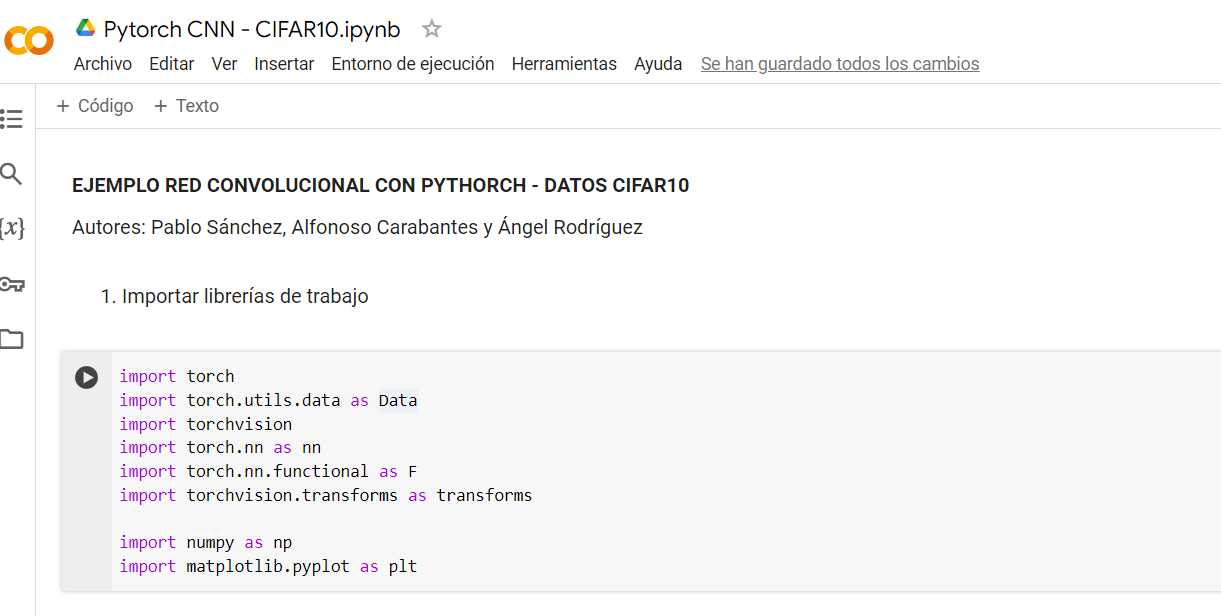
\includegraphics[keepaspectratio]{imagenes/capitulo1/colab_1.png}}\{\#fig-colab\_1{]}

Este es el menú principal de colab desde donde podemos gestionar
nuestros proyectos:

\pandocbounded{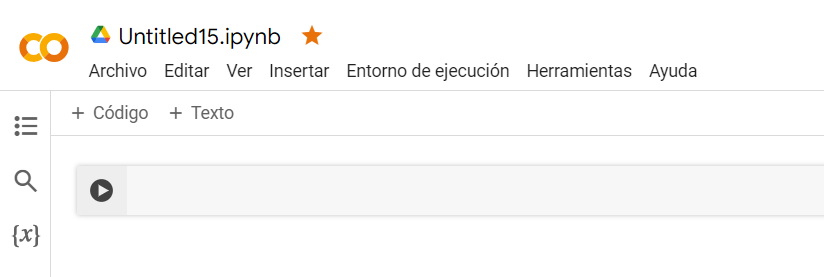
\includegraphics[keepaspectratio]{imagenes/capitulo1/colab_nuevo_fichero.png}}\{\#fig-colab\_nuevo\_fichero{]}

Desde el \texttt{menú\ Archivo}, como en la mayor parte de los
programas, podemos llevar a cabo las operaciones habituales de abrir y
guardar los ficheros en diferentes formatos. En este caso se pueden
abrir ficheros de Jupyter/Python desde cualquier dispositivo externo,
desde el repositorio Drive o de Github:

\pandocbounded{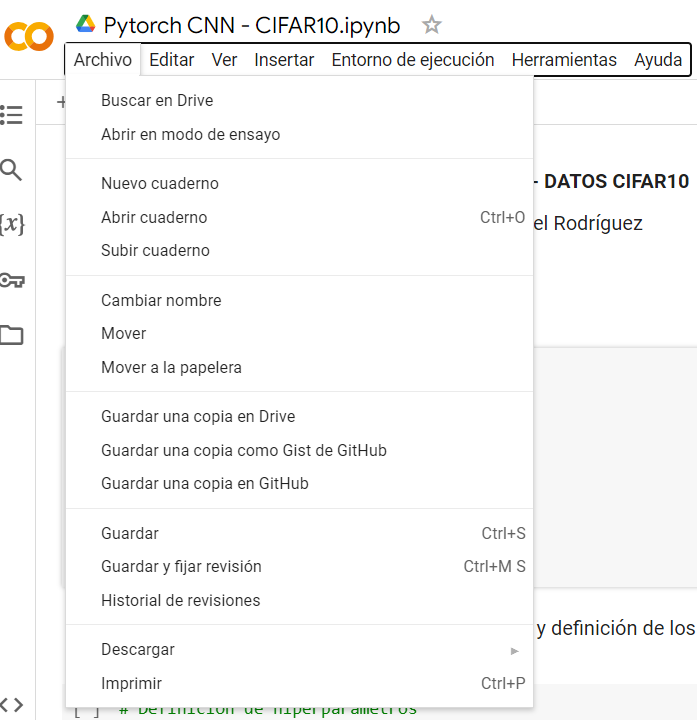
\includegraphics[keepaspectratio]{imagenes/capitulo1/colab_importa.png}}\{\#fig-colab\_importa{]}

Si queremos subir un fichero que tenemos en nuestro ordenador vamos a
\texttt{Archivo/Subir} cuaderno y podemos elegir nuestro archivo cuando
se despliegue la siguiente pantalla:

\pandocbounded{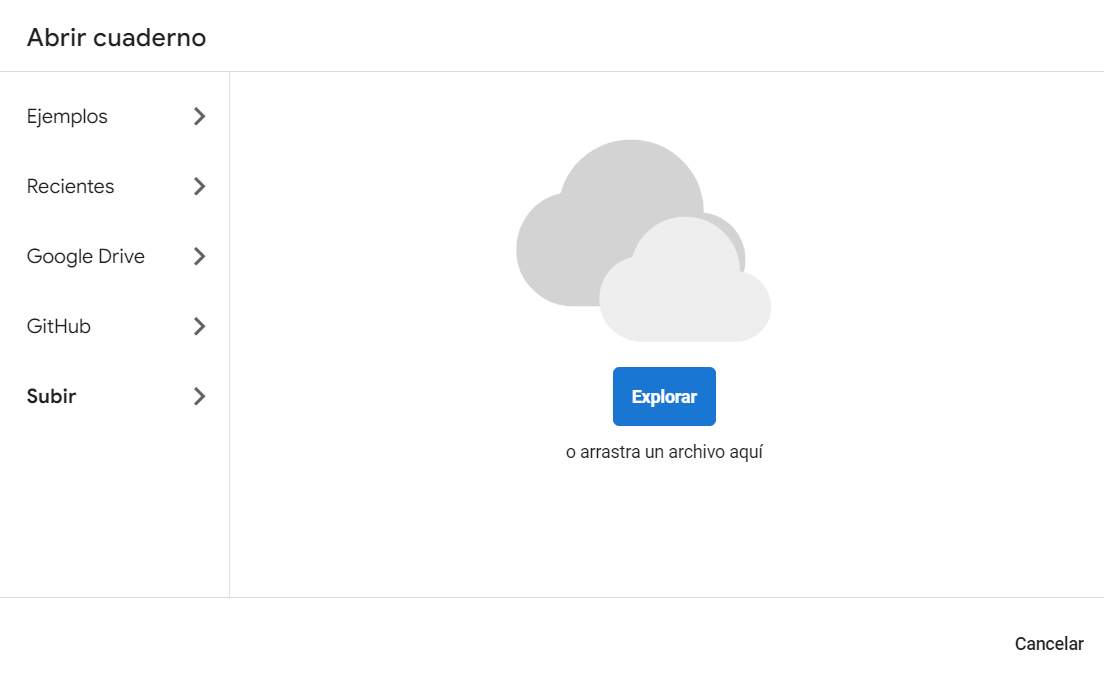
\includegraphics[keepaspectratio]{imagenes/capitulo1/colab_importa_archivo.png}}\{\#fig-colab\_importa\_archivo{]}

Como se ha comentado también se pueden importar archivos desde GitHub
introduciendo la url de GitHub:

\pandocbounded{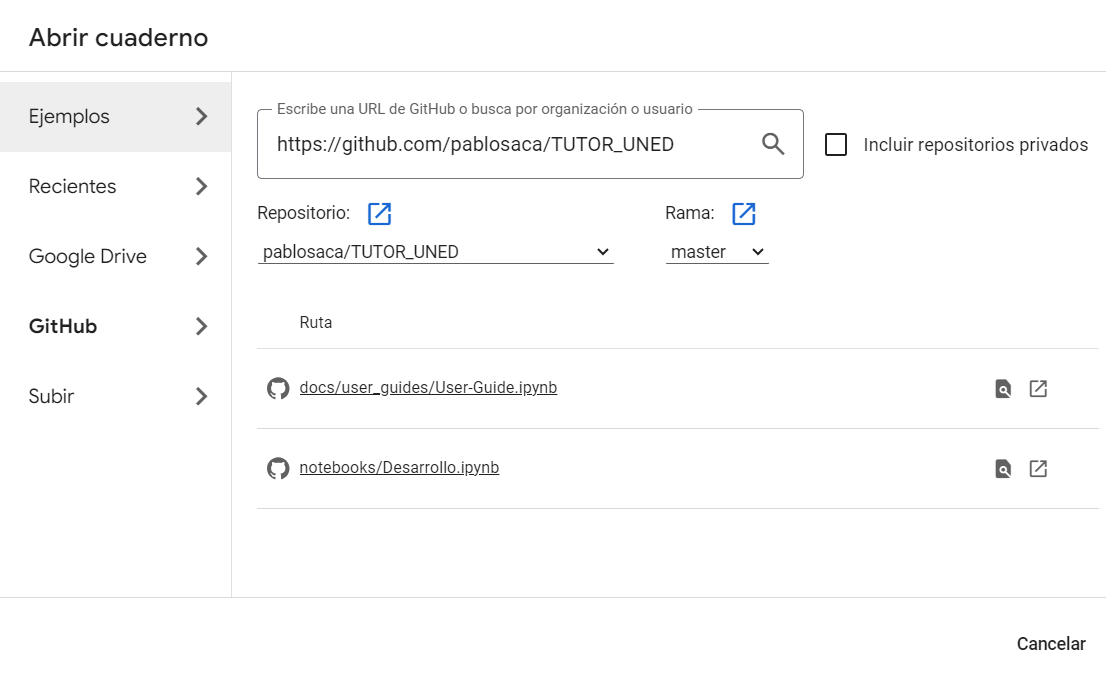
\includegraphics[keepaspectratio]{imagenes/capitulo1/colab_importa_github.png}}\{\#fig-colab\_importa\_github{]}

Por último, \emph{colab} nos permite tener acceso tanto a GPUs de forma
como a CPUs más potentes que nuestro ordenador de escritorio de forma
gratuita.

\pandocbounded{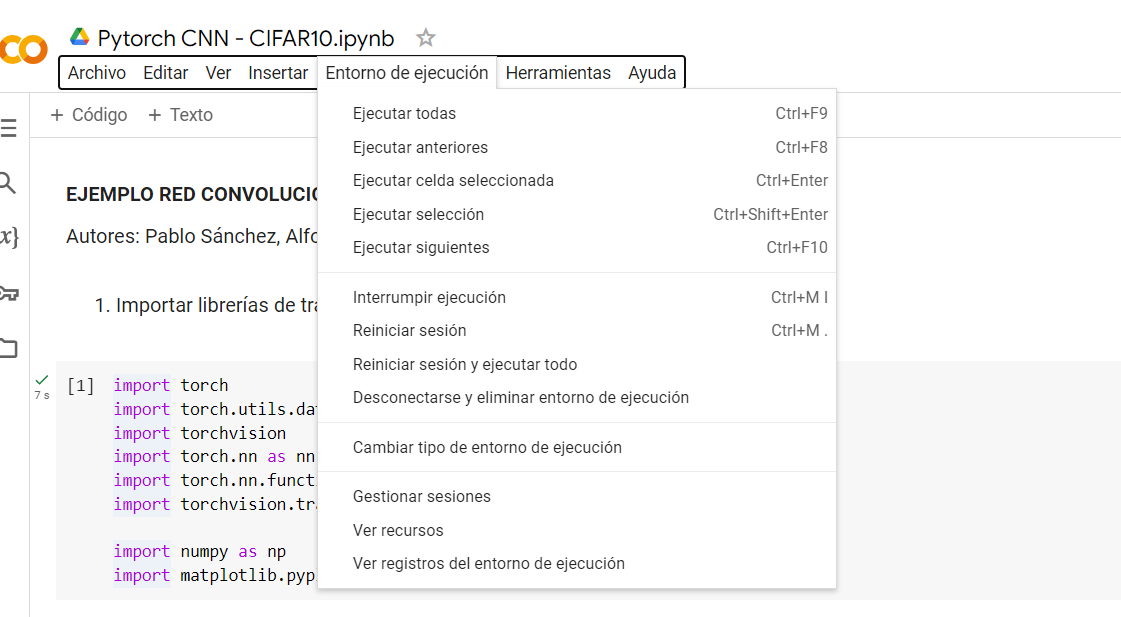
\includegraphics[keepaspectratio]{imagenes/capitulo1/colab_entorno_ejecucion_inicio.png}}\{\#fig-colab\_entorno\_ejecucion\_inicio{]}

\section{Conceptos básicos de las Redes
Neuronales}\label{conceptos-buxe1sicos-de-las-redes-neuronales}

Vamos a hacer una revisión de las redes neuronales para posteriormente
poder abordar los diferentes tipos de redes neuronales que se utilizan
en Deep Learning. Algunos de los avances más recientes en varios de los
diferentes componentes que forman parte de las redes neuronales están
recopilados en (Gu et al.~2017)

Las redes neuronales artificiales tienen sus orígenes en el Perceptrón,
que fue el modelo creado por Frank Rosenblatt en 1957 y basado en los
trabajos que previamente habían realizado Warren McCullon
(neurofisiólogo) y Walter Pitts (matemático).

El Perceptrón está construido por una neurona artificial cuyas entradas
y salida pueden ser datos numéricos, no como pasaba con la neurona de
McCulloch y Pitts (eran sólo datos lógicos). Las neuronas pueden tener
pesos y además se le aplica una función de activación Sigmoid (a
diferencia de la usada anteriormente al Paso binario).

En esta neurona nos encontramos que se realizan los siguientes cálculos:
\[ z = \sum_{i=1}^{n}w_ix_i+b_i\] \[\hat{y} = \delta (z)\] donde
representan los datos numéricos de entrada, son los pesos, es el sesgo
(bias), es la función de activación y finalmente es el dato de salida.

El modelo de perceptrón es el más simple, en el que hay una sola capa
oculta con una única neurona.

El siguiente paso nos lleva al Perceptrón Multicapa donde ya pasamos a
tener más de una capa oculta, y además podemos tener múltiples neuronas
en cada capa oculta.

Cuando todas las neuronas de una capa están interconectadas con todas
las de la siguiente capa estamos ante una red neuronal densamente
conectada. A lo largo de las siguientes secciones nos encontraremos con
redes en las que no todas las neuronas de una capa se conectan con todas
de la siguiente.

Veamos como describiríamos ahora los resultados de las capas \[
z_j^{(l)}=\sum_{i=1}^{n_j} w_{i j}^{(l)} a_i^{(l-1)}+b_i^{(l)} \\
a_j^{(l)}=\delta^{(l)}\left(z_j^{(l)}\right)
\] donde \(a_i^{(l-1)}\) representan los datos de la neurona \(i\) en la
capa \(l-1\) ( siendo \(a_i^0=x_i\) los valores de entrada),
\(w_{i j}^{(l)}\) son los pesos en la capa \(l\), \(b_i^{(l)}\) es el
sesgo (bias) en la capa \(l\), \(\delta^{(l)}\) es la función de
activación en la capa \(l\) (puede que cada capa tenga una función de
activación diferente), \(n_j\) es el número de neurona de la capa
anterior que conectan con la \(j\) y finalmente \(a_j^{(l)}\) es el dato
de salida de la capa \(l\). Es decir, en cada capa para calcular el
nuevo valor necesitamos usar los valores de la capa anterior.

\textbf{Aplicaciones de las Redes Neuronales}

Cada día las redes neuronales están más presentes en diferentes campos y
ayudan a resolver una gran variedad de problemas. Podríamos pensar que
de forma más básica una red neuronal nos puede ayudar a resolver
problemas de regresión y clasificación, es decir, podríamos considerarlo
como otro modelo más de los existentes que a partir de unos datos de
entrada somos capaces de obtener o un dato numérico (o varios) para
hacer una regresión (calcular en precio de una vivienda en función de
diferentes valores de la misma) o que somos capaces de conseguir que en
función de los datos de entrada nos deje clasificada una muestra
(decidir si conceder o no una hipoteca en función de diferentes datos
del cliente).

Si los datos de entrada son imágenes podríamos estar usando las redes
neuronales como una forma de identificar esa imagen:

\begin{itemize}
\item
  Identificando que tipo de animal es
\item
  Identificando que señal de tráfico es
\item
  Identificando que tipo de fruta es
\item
  Identificando que una imagen es de exterior o interior de una casa
\item
  Identificando que es una cara de una persona
\item
  Identificando que una imagen radiográfica represente un tumor maligno
\item
  Identificando que haya texto en una imagen
\end{itemize}

Luego podríamos pasar a revolver problemas más complejos combinando las
capacidades anteriores:

\begin{itemize}
\item
  Detectar los diferentes objetos y personas que se encuentran en una
  imagen
\item
  Etiquedado de escenas (aula con alumnos, partido de futbol, etc\ldots)
\end{itemize}

Después podríamos dar el paso al video que lo podríamos considerar como
una secuencia de imágenes:

\begin{itemize}
\item
  Contar el número de personas que entran y salen de una habitación
\item
  Reconocer que es una carretera
\item
  Identificar las señales de tráfico
\item
  Detectar si alguien lleva un arma
\item
  Seguimiento de objetos
\item
  Detección de estado/actitud de una persona
\item
  Reconocimiento de acciones (interpretar lenguaje de signos,
  interpretar lenguaje de banderas)
\item
  Vehículos inteligentes
\end{itemize}

Si los datos de entrada son secuencias de texto

\begin{itemize}
\item
  Sistemas de traducción - Chatbots (resolución de preguntas a usuarios)
\item
  Conversión de texto a audio
\end{itemize}

Si los datos de entrada son audios

\begin{itemize}
\item
  Sistemas de traducción
\item
  Altavoces inteligentes
\item
  Conversión de audio a texto
\end{itemize}

A continuación, pasamos a revisar diferentes elementos de las redes
neuronales que suelen ser comunes a todos los tipos de redes neuronales.

\subsection{Datos}\label{datos}

Cuando se trabaja con redes neuronales necesitamos representar los
valores de las variables de entrada en forma numérica. En una red
neuronal todos los datos son siempre numéricos. Esto significa que todas
aquellas variables que sean categóricas necesitamos convertirlas en
numéricas.

Además, es muy conveniente normalizar los datos para poder trabajar con
valores entre 0 y 1, que van a ayudar a que sea más fácil que se pueda
converger a la solución. Es importante que los datos seán números en
coma flotante, sobre todo si se van a trabajar con GPUs (Graphics
Process Units), ya que permitirán hacer un mejor uso de los multiples
cores que les permiten operar en coma flotante de forma paralela.
Actualmente, hay toda una serie de mejoras en las GPUs que permite
aumentar el rendimiento de las redes neuronales como son el uso de
operaciones en FP16 (Floating Point de 16 bits en lugar de 32) de forma
que pueden hacer dos operaciones de forma simultánea (el formato
estándar es FP32) y además con la reducción de memoria (punto muy
importante) al meter en los 32 bits 2 datos en lugar de sólo uno.
También se han añadido técnicas de Mixed Precision (Narang et al.~2018),
los Tensor Cores (para las gráficas de NVIDIA) son otra de las mejoras
que se han ido incorporando a la GPUs y que permiten acelerar los
procesos tanto de entrenamiento como de predicción con las redes
neuronales.

El primer objetivo será convertir las variables categóricas en variables
numéricas, de forma la red neuronal pueda trabajar con ellas. Para
realizar la conversión de categórica a numérica básicamente tenemos dos
métodos para realizarlo:

\begin{itemize}
\item
  Codificación one-hot.
\item
  Codificación entera.
\end{itemize}

La \textbf{codificación one-hot} consiste en crear tantas variables como
categorías tenga la variable, de forma que se asigna el valor 1 si tiene
esa categoría y el 0 si no la tiene.

La \textbf{codificación entera} lo que hace es codificar con un número
cada categoría. Realmente esta asignación no tiene ninguna
interpretación numérica ya que en general las categorías no tienen
porque representar un orden al que asociarlas.

Normalmente se trabaja con codificación one-hot para representar los
datos categóricos de forma que será necesario preprocesar los datos de
partida para realizar esta conversión, creando tantas variables como
categorías haya por cada variable.

Si nosotros tenemos nuestra muestra de datos que tiene \(n\) variables
\(x=\{x_1,x_2,...,x_n\}\) de forma que \(x_{n-2},x_{n-1},x_n\) son
variables categóricas que tienen \(k,l,m\) número de categorías
respectivamente, tendremos finalmente las siguientes variables sólo
numéricas:
\[ x=\{x_1,x_2,...,x_{(n-2)_1},...,x_{(n-2)_k},x_{(n-1)_1},...,x_{(n-1)_l},x_{n_1},...,x_{n_m}\} \]

De esta forma, se aumentarán el número de variables con las que vamos a
trabajar en función de las categorías que tengan las variables
categóricas. Normalmente nos encontramos que en una red neuronal las
variables de salida son:

\begin{itemize}
\tightlist
\item
  un número (regresión)
\item
  una serie de números (regresión múltiple)
\item
  un dato binario (clasificación binaria)
\item
  una serie de datos binarios que representa una categoría de varias
  (clasifiación múltiple)
\end{itemize}

\subsection{Arquitectura de red}\label{arquitectura-de-red}

Para la construcción de una red neuronal necesitamos definir la
arquitectura de esa red. Esta arquitectura, si estamos pensando en una
red neuronal densamente conectada, estará definida por la cantidad de
capas ocultas y el número de neuronas que tenemos en cada capa. Más
adelante veremos que dependiendo del tipo de red neuronal podrá haber
otro tipo de elementos en estas capas.

\subsection{Función de coste y
pérdida}\label{funciuxf3n-de-coste-y-puxe9rdida}

Otro de los elementos clave que tenemos que tener en cuenta a la hora de
usar nuestra red neuronal son las \textbf{funciones de pérdida y
funciones de coste (objetivo)}.

\textbf{La función de pérdida} va a ser la función que nos dice cómo de
diferente es el resultado del dato que nosotros queríamos conseguir
respecto al dato original. Normalmente se suelen usar diferentes tipos
de funciones de pérdida en función del tipo de resultado con el que se
vaya a trabajar.

\textbf{La función de coste} es la función que vamos a tener que
\textbf{optimizar} para conseguir el mínimo valor posible, y que recoge
el valor de la función de pérdida para toda la muestra.

Tanto las funciones de pérdida como las funciones de coste, son
funciones que devuelven valores de de \(\mathbb{R}\)..

Si tenemos un problema de \textbf{regresión} en el que tenemos que
predecir un valor o varios valores numéricos, algunas de las funciones a
usar son:

\begin{itemize}
\tightlist
\item
  \textbf{Error medio cuadrático} \(\left(\mathrm{L}_2^2\right)\)
\end{itemize}

\[
\mathcal{L}_{\text {MSE }}(\mathrm{y}, \hat{\mathrm{y}})=\|\hat{\mathrm{y}}-\mathrm{y}\|^2=\sum_{\mathrm{i}=1}^{\mathrm{n}}\left(\hat{\mathrm{y}}_{\mathrm{i}}-\mathrm{y}_{\mathrm{i}}\right)^2
\] donde \(\hat{y}\) y y son vectores de tamaño \(n, y\) es el valor
real e \(\hat{y}\) es el valor predicho

\begin{itemize}
\tightlist
\item
  \textbf{Error medio absoluto (} \(\mathrm{L}_1\) )
\end{itemize}

\[
\mathcal{L}_{\text {MAE }}(\mathrm{y}, \hat{y})=|\hat{y}-y|=\sum_{i=0}^n\left|\hat{y}_i-y_i\right|
\] donde \(\hat{y}\) y y son vectores de tamaño \(n, y\) es el valor
real e \(\hat{y}\) es el valor predicho

Para los problemas de \textbf{clasifiación}:

\begin{itemize}
\tightlist
\item
  \textbf{Binary Crossentropy (Sólo hay dos clases)} \[
  \mathcal{L}_{\text {CRE }}(\mathrm{y}, \hat{y})=-(\mathrm{y} \log (\hat{y})+(1-\mathrm{y}) \log (1-\hat{y}))
  \]
\end{itemize}

\(\mathrm{y}\) es el valor real e \(\hat{y}\) es el valor predicho

\begin{itemize}
\tightlist
\item
  \textbf{Categorical Crosentropy (Múltiples clases representadas como
  one-hot)}
\end{itemize}

\[
\mathcal{L}_{\text {CAE }}\left(\mathrm{y}_{\mathrm{c}}, \hat{\mathrm{y}}_{\mathrm{c}}\right)=-\sum_{\mathrm{c}=1}^{\mathrm{k}} \mathrm{y}_{\mathrm{c}} \log \left(\hat{y}_c\right)
\]

\(y_c\) es el valor real para la clase \(c\) e \(\hat{y}_c\) es el valor
predicho para la clase \(c\)

\begin{itemize}
\tightlist
\item
  \textbf{Sparse Categorical Crossentropy (Múltiples clases
  representadas comp un entero)}
\end{itemize}

\[
\mathcal{L}_{\text {SCAE }}\left(\mathrm{y}_{\mathrm{c}}, \hat{\mathrm{y}}_{\mathrm{c}}\right)=-\sum_{\mathrm{c}=1}^{\mathrm{k}} \mathrm{y}_{\mathrm{c}} \log \left(\hat{y}_{\mathrm{c}}\right)
\]

\(\mathrm{y}_c\) es el valor real para la clase \(c\) e \(\hat{y}_c\) es
el valor predicho para la clase \(c\)

\begin{itemize}
\tightlist
\item
  \textbf{Kullback-Leibler Divergence}
\end{itemize}

Esta función se usa para calcular la diferencia entre dos distribuciones
de probabilidad se usa por ejemplo en algunas redes como
\textbf{Variational Autoencoders} (Doersch 2016 Modelos GAN (Generative
Adversarial Networks)

\[
\mathcal{D}_{\mathrm{KL}}(\mathrm{p} \| \mathrm{q})=-\mathrm{H}(\mathrm{p}(\mathrm{x}))-\mathrm{E}_{\mathrm{p}}[\log \mathrm{q}(\mathrm{x})]
\]

\[
=\sum_x p(x) \operatorname{logp}(x)-\sum_x p(x) \log q(x)=\sum_x p(x) \log \frac{p(x)}{q(x)}
\]

\[
\mathcal{L}_{\text {vae }}(y, \hat{y})=E_{z \sim q_\phi(z \mid x)}\left[\operatorname{logp}_\theta(x \mid z)\right]-\mathcal{D}_{\text {KL }}\left(q_\phi(z \mid x) \| p(z)\right)
\]

\begin{itemize}
\tightlist
\item
  \textbf{Hinge Loss}
\end{itemize}

\[
\mathcal{L}_{\text {hinge }}(\mathrm{y}, \hat{y})=\max (0,1-\mathrm{y} * \hat{\mathrm{y}})
\]

Las correspondientes \textbf{funciones de coste} que se usarían,
estarían asociadas a todas las muestras que se estén entrenando o sus
correpondientes batch, así como posibles términos asociados a la
regularización para evitar el sobreajuste del entrenamiento. Es decir,
la función de pérdida se calcula para cada muestra, y la función de
coste es la media de todas las muestras.

Por ejemplo, para el \textbf{Error medio cuadrático}
\(\left(L_2\right)\) tendríamos el siguiente valor: \[
\mathcal{J}_{\text {MSB }}(y, \hat{y})=\frac{1}{m} \sum_{i=1}^m \mathcal{L}_{\text {MSE }}(y, \hat{y})=\frac{1}{m} \sum_{i=1}^m|| \hat{y}_i-y_i \|^2=\frac{1}{n} \sum_{i=1}^m \sum_{i=1}^n\left(\hat{y}_{j i}-y_{j i}\right)^2
\]

\subsection{Optimizador}\label{optimizador}

El \textbf{Descenso del gradiente} es la versión más básica de los
algoritmos que permiten el aprendizaje en la red neuronal haciendo el
proceso de \textbf{backpropagation} (propagación hacia atrás). A
continuación veremos una breve explicación del algoritmo así como
algunas variantes del mismo recogidas en (Ruder 2017).

Recordamos que el descenso del gradiente nos permitirá actualizar los
parámetros de la red neuronal cada vez que demos una pasada hacia
delante con todos los datos de entrada, volviendo con una pasada hacia
atrás.

\[\mathrm{w}_{\mathrm{t}}=\mathrm{w}_{\mathrm{t}-1}-\alpha \nabla_{\mathrm{w}} \mathcal{J}(\mathrm{w})\]

donde \(\mathcal{J}\) es la \textbf{función de coste}, \(\alpha\) es el
parámetro de \textbf{ratio de aprendizaje} que permite definir como de
grandes se quiere que sean los pasos en el aprendizaje.

Cuando lo que hacemos es actualizar los parámetros para cada pasada
hacia delante de una sola muestra, estaremos ante lo que llamamos
\textbf{Stochastic Gradient} Descent (SGD). En este proceso convergerá
en menos iteraciones, aunque puede tener alta varianza en los
parámetros.

\[\mathrm{W}_{\mathrm{t}}=\mathrm{w}_{\mathrm{t}-1}-\alpha \nabla_{\mathrm{w}} \mathcal{J}(\mathrm{w}, x(i),y(i))\]

donde \(x(i)\) e \(y(i)\) son los valores en la pasada de la muestra
\(i\).

Podemos buscar un punto intermedio que sería cuando trabajamos por lotes
y cogemos un bloque de datos de la muestra, les aplicamos la pasada
hacia delante y aprendemos los parámetros para ese bloque. En este caso
lo llamaremos \textbf{Mini-batch Gradient Descent}

\[\mathrm{W}_{\mathrm{t}}=\mathrm{w}_{\mathrm{t}-1}-\alpha \nabla_{\mathrm{w}} \mathcal{J}(\mathrm{w}, \mathrm{B}(\mathrm{i}))\]

donde \(\mathrm{B}(\mathrm{i})\) son los valores de ese batch .

En general a estos métodos nos referiremos a ellos como \textbf{SGD}.

Sobre este algoritmo base se han hecho ciertas mejoras como:

\textbf{Learning rate decay} Podemos definir un valor de decenso del
ratio de aprendizaje, de forma que normalmente al inicio de las
iteraciones de la red neuronal los pasos serán más grandes, pero
conforme nos acercamos a la solución optima deberemos dar pasos más
pequeños para ajustarnos mejor.

\[\mathrm{W}_{\mathrm{t}}=\mathrm{w}_{\mathrm{t}-1}-\alpha_{\mathrm{t}} \nabla_{\mathrm{w}} \mathcal{J}\left(\mathrm{w}_{\mathrm{t}-1}\right)\]

donde \(\alpha _t\) ahora se irá reduciendo en función del valor del
\textbf{decay}.

\textbf{Momentum} El \textbf{momentum} se introdujo para suavizar la
convergencia y reducir la alta varianza de SGD.

\[ V_ {t}  =  \gamma   v_ {t-1}  +  \alpha  V_ {w} J(  w_ {t-1}  ,x,y)\]
\[ W_ {t} =  w_ {t-1}  -  v_ {1} \]

donde \(v_t\) es lo que se llama el \textbf{vector velocidad} con la
dirección correcta.

\textbf{NAG (Nesterov Accelerated Gradient)} Ahora daremos un paso más
con el NAG, calculando la función de coste junto con el vector
velocidad.

\[ V_ {t}  =  \gamma   v_ {t-1}  +  \alpha   V_ {w}  J(  w_ {t-1}  -  \gamma   v_ {t-1}  ,x,y) \]
\[ W_ {t}  =  w_ {t-1}  -  v_ {t}  \]

donde ahora vemos que la función de coste se calcula usando los
parámetros de \(w_t\) sumado a \(\gamma   v_ {t-1}\)

Veamos algunos algoritmos de optimización más que, aunque provienen del
SGD, se consideran independientes a la hora de usarlos y no como
parámetros extras del SGD.

\textbf{Adagrad (Adaptive Gradient)} Esta variante del algoritmo lo que
hace es adaptar el ratio de aprendizaje para cada uno de los pesos en
lugar de que sea global para todos.

\[ W_ {t,i}  =  w_ {t-1,i}  -  \frac {\alpha }{\sqrt {G_ {t-1,i,j}+\epsilon }}   \nabla_ {w_{t-1}}  J(  w_ {t-1,i} ,x,y) \]

donde tenemos que \(G_t \in R^{dxd}\)\$es una matriz diagonal donde cada
elemento es la suma de los cuadrados de los gradientes en el paso
\(t-1\) , y es un término de suavizado para evitar divisiones por 0.

\textbf{RMSEProp (Root Mean Square Propagation)} En este caso tenemos
una variación del Adagrad en el que intenta reducir su agresividad
reduciendo monotonamente el ratio de aprendizaje. En lugar de usar el
gradiente acumulado desde el principio de la ejecución, se restringe a
una ventana de tamaño fijo para los últimos n gradientes calculando su
media. Así calcularemos primero la media en ejecución de los cuadros de
los gradientes como:

\[
\mathrm{E}\left[g^2\right]_{t-1}=\gamma E\left[g^2\right]_{t-2}+(1-\gamma) g_{t-1}^2
\]

y luego ya pasaremos a usar este valor en la actualización

\[
w_{t, i}=w_{t-1, i}-\frac{\alpha}{\sqrt{E\left[ g^2\right]_{t-1}+\epsilon}} \nabla_{w_{t-1}} \mathcal{J}\left(w_{t-1, i}, x, y\right)
\]

\textbf{AdaDelta}

Aunque se desarrollaron de forma simultánea el AdaDelta y el RMSProp son
muy parecidos en su primer paso incial, llegando el de AdaDelta un poco
más lejos en su desarrollo.

\[
w_{t, i}=w_{t-1, i}-\frac{\alpha}{\sqrt{E\left[ g^2\right]_{t-1}+\epsilon}} \nabla_{w_{t-1}} \mathcal{J}\left(w_{t-1, i}, x, y\right)
\]

y luego ya pasaremos a usar este valor en la actualización

\[
\begin{gathered}w_{t, i}=w_{t-1, i}-\frac{\alpha}{\sqrt{E\left[g^2\right]_{t-1}+\epsilon}} \nabla_{w_{t-1}} \mathcal{J}\left(w_{\mathrm{t}-1, \mathrm{i}}, \mathrm{X}, \mathrm{y}\right) \\ \Delta w_{\mathrm{t}}=-\frac{\alpha}{\sqrt{\mathrm{E}\left[g^2\right]_{\mathrm{t}}+\epsilon}} g_t\end{gathered}
\]

\textbf{Adam (Adaptive Moment Estimation)}

\[
\begin{gathered}G_t=\nabla_{w_t} \mathcal{J}\left(w_t\right) \\ M_{t-1}=\beta_1 m_{t-2}+\left(1-\beta_1\right) g_{t-1} \\ v_{t-1}=\beta_2 v_{t-2}+\left(1-\beta_2\right) g_{t-1}^2\end{gathered}
\]

donde \(m_{t-1}\) y \(V_{t-1}\) son estimaciones del primer y segundo
momento de los gradientes respectivamente, y \(\beta_1\) y \(\beta_2\)
parámetros a asignar.

\[\widehat{M}_{t-1}  =\frac{m_{t-1}}{1-\beta_1^{t-1}} \\  \widehat{V}_{t-1}  =\frac{v_{t-1}}{1-\beta_2^{t-1}} \\  W_t=w_{t-1}  -\frac{\alpha}{\sqrt{\hat{v}_{t-1}+\epsilon}} \widehat{m}_{t-1}\]

\textbf{Adamax}

\[
G_t=\nabla_{w_t} \mathcal{J}\left(w_t\right) \\ 
M_{t-1}=\beta_1 m_{t-2}+\left(1-\beta_1\right) g_{t-1} \\ 
\mathrm{~V}_{\mathrm{t}-1}=\beta_2 \mathrm{v}_{\mathrm{t}-2}+\left(1-\beta_2\right) \mathrm{g}_{\mathrm{t}-1}^2 \\ 
\mathrm{U}_{\mathrm{t}-1}=\max \left(\beta_2 \cdot \mathrm{v}_{\mathrm{t}-1},\left|\mathrm{~g}_{\mathrm{t}}\right|\right)
\]

donde \(m_{t-1}\) y \(V_{t-1}\) son estimaciones del primer y segundo
momento de los gradientes respectivamente, y \(\beta_1\) y \(\beta_2\)
parámetros a asignar.

\[
\widehat{M}_{t-1}=\frac{m_{t-1}}{1-\beta_1^{t-1}} \\ 
W_t=w_{t-1}-\frac{\alpha}{u_{t-1}} \widehat{m}_{t-1}
\]

\textbf{Nadam (Nesterov-accelerated Adaptive Moment Estimatio)} Combina
Adam y NAG.

\[
\begin{aligned} G_t & =\nabla_{w_t} \mathcal{J}\left(w_t\right) \\ M_{t-1} & =\gamma m_{t-2}+\alpha g_{t-1} \\ w_t & =w_{t-1}-m_{t-1}\end{aligned}
\]

\subsection{Función de activación}\label{funciuxf3n-de-activaciuxf3n}

Las funciones de activación dentro de una red neuronal son uno de los
elementos clave en el diseño de la misma. Cada tipo de función de
activación podrá ayudar a la convergencia de forma más o menos rápida en
función del tipo de problema que se plantee. En una red neuronal las
funciones de activación en las capas ocultas van a conseguir establecer
las restricciones \textbf{no lineales} al pasar de una capa a la
siguiente, normalmente se evita usar la función de activación lineal en
las capas intermedias ya que queremos conseguir transformaciones no
lineales.

A continuación, exponemos las principales funciones de activación en las
capas ocultas:

\begin{itemize}
\tightlist
\item
  \textbf{Paso binario} (Usado por los primeros modelos de neuronas)
\end{itemize}

\(F(x)= \begin{cases}0 & \text { for } x \leq 0 \\ x & \text { for } x>0\end{cases}\)

\begin{itemize}
\tightlist
\item
  \textbf{Identidad}
\end{itemize}

\(F(x)=x\)

\begin{itemize}
\tightlist
\item
  \textbf{Sigmoid (Logística)}
\end{itemize}

\(F(x)=\frac{1}{1+e^{-x}}\)

\begin{itemize}
\tightlist
\item
  \textbf{Tangente Hiperbólica (Tanh)}
\end{itemize}

\(F(x)=\tanh (x)=\frac{\left(e^x-e^{-x}\right)}{\left(e^x+e^{-x}\right)}\)

\begin{itemize}
\tightlist
\item
  \textbf{Softmax}
\end{itemize}

\(F\left(x_i\right)=\frac{e^{x_i}}{\sum_{j=0}^k e^{x_j}}\)

\begin{itemize}
\item
  \textbf{ReLu ( Rectified Linear Unit)}
  \(\begin{aligned} & F(x)=\max (0, x) \\ & f(x)= \begin{cases}0 & \text { for } x \leq 0 \\ x & \text { for } x>0\end{cases} \end{aligned}\)
\item
  \textbf{LReLU (Leaky Rectified Linear Unit)}
  \(F(\alpha, x)= \begin{cases}\alpha x & \text { for } x<0 \\ x & \text { for } x \geq 0\end{cases}\)
\item
  \textbf{PReLU (Parametric Rectified Linear Unit)}
  \(F(\alpha, x)= \begin{cases}\alpha x & \text { for } x<0 \\ x & \text { for } x \geq 0\end{cases}\)
\item
  \textbf{RReLU (Randomized Rectified Linear Unit)}
  \(F(\alpha, x)= \begin{cases}\alpha x & \text { for } x<0 \\ x & \text { for } x \geq 0\end{cases}\)
\end{itemize}

*La diferencia entre LReLu, PReLu y RRLeLu es que en LReLu el parámetro
es uno que se asigna fijo, en el caso de PReLu el parámetro también se
aprende durante el entrenamiento y finalmente en RReLu es un parámetro
con valores entre 0 y 1, que se obtiene de un muestreo en una
distribución normal.

Se puede profundizar en este grupo de funciones de activación en (Xu et
al.~2015)

\begin{itemize}
\tightlist
\item
  ELU (Exponential Linear Unit)
  \(F(\alpha, x)= \begin{cases}\alpha\left(e^{x-1}\right) & \text { for } x<0 \\ x & \text { for } x \geq 0\end{cases}\)
\end{itemize}

\begin{figure}

\centering{

\pandocbounded{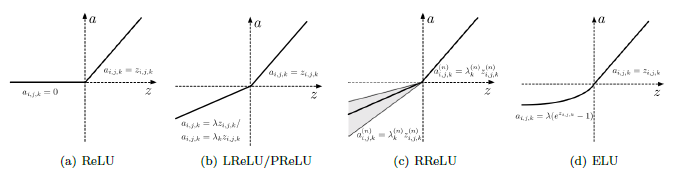
\includegraphics[keepaspectratio]{imagenes/capitulo1/funciones_activacion.png}}

}

\caption{\label{fig-funciones_activacion}Funciones ReLU}

\end{figure}%

\textbf{Función de activación en salida}

En la capa de salida tenemos que tener en cuenta cual es el tipo de
datos final que queremos obtener, y en función de eso elegiremos cual es
la función de activación de salida que usaremos. Normalmente las
funciones de activación que se usarán en la última capa seran:

\begin{itemize}
\item
  \textbf{Lineal} con una unidad, para regresión de un solo dato
  numérico \(F(x)=x\) donde es un valor escalar.
\item
  \textbf{Lineal} con multiples unidades, para regresión de varios datos
  numéricos \(F(x)=x\) donde \(x\) es un vector.
\item
  \textbf{Sigmoid} para clasifiación binaria \(F(x)=\frac{1}{1+e^{-x}}\)
\item
  \textbf{Softmax} para calsifiación múltiple
  \(F\left(x_i\right)=\frac{e^{x_i}}{\sum_{j=0}^k e^{x_j}}\)
\end{itemize}

\subsection{Regularización}\label{regularizaciuxf3n}

Las técnicas de regularización nos permiten conseguir mejorar los
problemas que tengamos por sobreajuste en el entrenamiento de nuestra
red neuronal.

A continuación, vemos algunas de las técnicas de regularización
existentes en la actualidad:

\begin{itemize}
\tightlist
\item
  \textbf{Norma LP} Básicamente estos métodos tratan de hacer que los
  pesos de las neuronas tengan valores muy pequeños consiguiendo una
  distribución de pesos más regular. Esto lo consiguen al añadir a la
  función de pérdida un coste asociado a tener pesos grandes en las
  neuronas. Este peso se puede construir o bien con la \textbf{norma L1}
  (proporcional al valor absoluto) o con la \textbf{norma L2}
  (proporcional al cuadrado de los coeficientes de los pesos). En
  general se define la norma LP) \[
  \begin{gathered}
  E(w, \mathbf{y}, \hat{\mathbf{y}})=\mathcal{L}(w, \mathbf{y}, \hat{\mathbf{y}})+\lambda R(w) \\
  R(w)=\sum_j\left\|w_j\right\|_p^p
  \end{gathered}
  \]
\end{itemize}

Para los casos más habituales tendríamos la norma \(\mathbf{L 1}\) y
\(\mathbf{L 2}\). \[
\begin{aligned}
& R(w)=\sum_j\left\|w_j\right\|^2 \\
& R(w)=\sum_j\left|w_j\right|
\end{aligned}
\]

\subsection{Dropout}\label{dropout}

Una de las técnicas de regularización que más se están usando
actualmente es la llamada \textbf{Dropout}, su proceso es muy sencillo y
consiste en que en cada iteración de forma aleatoria se dejan de usar un
porcentaje de las neuronas de esa capa, de esta forma es más difícil
conseguir un sobreajuste porque las neuronas no son capaces de memorizar
parte de los datos de entrada.

\subsection{Dropconnect}\label{dropconnect}

El Dropconnect es otra técnica que va un poco más allá del concepto de
Dropout y en lugar de usar en cada capa de forma aleatoria una serie de
neuronas, lo que se hace es que de forma aleatoria se ponen los pesos de
la capa a cero. Es decir, lo que hacemos es que hay ciertos enlaces de
alguna neurona de entrada con alguna de salida que no se activan.

\subsection{Inicialización de pesos}\label{inicializaciuxf3n-de-pesos}

Cuando empieza el entrenamiento de una red neuronal y tiene que realizar
la primera pasada hacia delante de los datos, necesitamos que la red
neuronal ya tenga asignados algún valor a los pesos.

Se pueden hacer inicializaciones del tipo:

\begin{itemize}
\item
  \textbf{Ceros} Todos los pesos se inicializan a 0.
\item
  \textbf{Unos} Todos los pesos se inicializan a 1.
\item
  \textbf{Distribución normal}. Los pesos se inicializan con una
  distribución normal, normalmente con media 0 y una desviación
  alrededor de 0,05. Es decir, valores bastante cercanos al cero.
\item
  \textbf{Distribución normal truncada}. Los pesos se inicializan con
  una distribución normal, normalmente con media 0 y una desviación
  alrededor de 0,05 y además se truncan con un máximo del doble de la
  desviación. Los valores aun són más cercanos a cero.
\item
  \textbf{Distribución uniforme}. Los pesos se inicializan con una
  distribución uniforme, normalmente entre el 0 y el 1.
\item
  \textbf{Glorot Normal} (También llamada Xavier normal) Los pesos se
  inicializan partiendo de una distribución normal truncada en la que la
  desivación es donde es el número de unidades de entrada y fanout es el
  número de unidades de salida. Ver (Glorot and Bengio 2010)
\item
  \textbf{Glorot Uniforme} (También llamada Xavier uniforme) Los pesos
  se inicializan partiendo de una distribución uniforme donde los
  límites son \([-\) limit,+ limit \(]\) done limit
  \(=\sqrt{\frac{6}{\text { fanin }+ \text { fanout }}}\) done \(fanin\)
  y es el número de unidades de entrada y \(fanout\) es el número de
  unidades de salida. Ver (Glorot and Bengio 2010)
\end{itemize}

\subsection{Batch normalization}\label{batch-normalization}

Hemos comentado que cuando entrenamos una red neuronal los datos de
entrada deben ser todos de tipo numérico y además los normalizamos para
tener valores ``cercanos a cero'', teniendo una media de 0 y varianza de
1, consiguiendo uniformizar todas las variables y conseguir que la red
pueda converger más fácilmente.

Cuando los datos entran a la red neuronal y se comienza a operar con
ellos, se convierten en nuevos valores que han perdido esa propiedad de
normalización. Lo que hacemos con la normalización por lotes (batch
normalization) (Ioffe and Szegedy 2015) es que añadimos un paso extra
para normalizar las salidas de las funciones de activación. Lo normal es
que se aplicara la normalización con la media y la varianza de todo el
bloque de entrenamiento en ese paso, pero normalmente estaremos
trabajando por lotes y se calculará la media y varianza con ese lote de
datos.

\subsection{Ejemplo de Red Neuronal con
Keras}\label{ejemplo-de-red-neuronal-con-keras}

\begin{Shaded}
\begin{Highlighting}[numbers=left,,]

\CommentTok{\# Importamos las librerías de keras/tensorflow}
\ImportTok{from}\NormalTok{ tensorflow }\ImportTok{import}\NormalTok{ keras}
\ImportTok{from}\NormalTok{ tensorflow.keras }\ImportTok{import}\NormalTok{ layers}

\CommentTok{\# Importamos la librería de los datasets de keras y cogemos el de boston\_housing}
\ImportTok{from}\NormalTok{ tensorflow.keras.datasets }\ImportTok{import}\NormalTok{ boston\_housing}

\CommentTok{\# Obtenemos los datos de entrenamiento y test}
\CommentTok{\# separados en las variables explicativas y la objetivo}
\NormalTok{(train\_data, train\_targets), (test\_data, test\_targets) }\OperatorTok{=}\NormalTok{ boston\_housing.load\_data()}
\NormalTok{train\_data.shape}
\NormalTok{test\_data.shape}

\CommentTok{\# Realizamos la "Normalización" restando la media y dividiendo por la desviación típica}
\CommentTok{\# Ahora tendremos valores ({-}x,x) alredor de 0, pero en general pequeños}
\NormalTok{mean }\OperatorTok{=}\NormalTok{ train\_data.mean(axis}\OperatorTok{=}\DecValTok{0}\NormalTok{)}
\NormalTok{train\_data }\OperatorTok{{-}=}\NormalTok{ mean}
\NormalTok{std }\OperatorTok{=}\NormalTok{ train\_data.std(axis}\OperatorTok{=}\DecValTok{0}\NormalTok{)}
\NormalTok{train\_data }\OperatorTok{/=}\NormalTok{ std}
\NormalTok{test\_data }\OperatorTok{{-}=}\NormalTok{ mean}
\NormalTok{test\_data }\OperatorTok{/=}\NormalTok{ std}

\CommentTok{\# Creamos el modelo}

\CommentTok{\# Inicializamos el API Secuencial de capas}
\NormalTok{model }\OperatorTok{=}\NormalTok{ keras.Sequential([}
        \CommentTok{\# Añadimos capa de entrada con las 13 variables explicativas}
\NormalTok{        keras.Input(shape}\OperatorTok{=}\NormalTok{(}\DecValTok{13}\NormalTok{,)),}
        \CommentTok{\# Añadimos capa densamente conectada con 64 neuronas y activación relu}
\NormalTok{        layers.Dense(}\DecValTok{64}\NormalTok{, activation}\OperatorTok{=}\StringTok{"relu"}\NormalTok{),}
        \CommentTok{\# Añadimos capa densamente conectada con 64 neuronas y activación relu}
\NormalTok{        layers.Dense(}\DecValTok{64}\NormalTok{, activation}\OperatorTok{=}\StringTok{"relu"}\NormalTok{),}
        \CommentTok{\# Añadimos capa de salida densamente conectada con 1 neurona y activación lineal (para regresión)}
\NormalTok{        layers.Dense(}\DecValTok{1}\NormalTok{)}
\NormalTok{    ])}

\CommentTok{\# Mostramos el Modelo creado}
\NormalTok{model.summary()}

\CommentTok{\# Compilamos el modelo definiendo el optimizador, función de pérdida y métrica}
\CommentTok{\# RMSProp, mse, mae}
\NormalTok{model.}\BuiltInTok{compile}\NormalTok{(optimizer}\OperatorTok{=}\StringTok{"rmsprop"}\NormalTok{, loss}\OperatorTok{=}\StringTok{"mse"}\NormalTok{, metrics}\OperatorTok{=}\NormalTok{[}\StringTok{"mae"}\NormalTok{])}



\CommentTok{\# Realizamos el entrenamiento}
\CommentTok{\# 130 épocos (iteraciones), con tamaño de batch de 16}
\NormalTok{history }\OperatorTok{=}\NormalTok{ model.fit(train\_data, train\_targets,}
\NormalTok{          epochs}\OperatorTok{=}\DecValTok{130}\NormalTok{, batch\_size}\OperatorTok{=}\DecValTok{16}\NormalTok{, verbose}\OperatorTok{=}\DecValTok{0}\NormalTok{)}


\CommentTok{\# Importamos la librería de pyplot para pintar gráficas}
\ImportTok{import}\NormalTok{ matplotlib.pyplot }\ImportTok{as}\NormalTok{ plt}

\CommentTok{\# list all data in history}
\BuiltInTok{print}\NormalTok{(history.history.keys())}
\CommentTok{\# summarize history for accuracy}
\NormalTok{plt.plot(history.history[}\StringTok{\textquotesingle{}mae\textquotesingle{}}\NormalTok{])}
\CommentTok{\#plt.plot(history.history[\textquotesingle{}val\_mae\textquotesingle{}])}
\NormalTok{plt.title(}\StringTok{\textquotesingle{}model mae\textquotesingle{}}\NormalTok{)}
\NormalTok{plt.ylabel(}\StringTok{\textquotesingle{}mae\textquotesingle{}}\NormalTok{)}
\NormalTok{plt.xlabel(}\StringTok{\textquotesingle{}epoch\textquotesingle{}}\NormalTok{)}
\NormalTok{plt.legend([}\StringTok{\textquotesingle{}train\textquotesingle{}}\NormalTok{, }\StringTok{\textquotesingle{}test\textquotesingle{}}\NormalTok{], loc}\OperatorTok{=}\StringTok{\textquotesingle{}upper left\textquotesingle{}}\NormalTok{)}
\NormalTok{plt.show()}
\CommentTok{\# summarize history for loss}
\NormalTok{plt.plot(history.history[}\StringTok{\textquotesingle{}loss\textquotesingle{}}\NormalTok{])}
\CommentTok{\#plt.plot(history.history[\textquotesingle{}val\_loss\textquotesingle{}])}
\NormalTok{plt.title(}\StringTok{\textquotesingle{}model loss\textquotesingle{}}\NormalTok{)}
\NormalTok{plt.ylabel(}\StringTok{\textquotesingle{}loss\textquotesingle{}}\NormalTok{)}
\NormalTok{plt.xlabel(}\StringTok{\textquotesingle{}epoch\textquotesingle{}}\NormalTok{)}
\NormalTok{plt.legend([}\StringTok{\textquotesingle{}train\textquotesingle{}}\NormalTok{, }\StringTok{\textquotesingle{}test\textquotesingle{}}\NormalTok{], loc}\OperatorTok{=}\StringTok{\textquotesingle{}upper left\textquotesingle{}}\NormalTok{)}
\NormalTok{plt.show()}


\CommentTok{\# Evaluamos el modelo con los datos de test}
\NormalTok{predictions }\OperatorTok{=}\NormalTok{ model.predict(test\_data)}
\NormalTok{predictions[}\DecValTok{0}\NormalTok{]}
\end{Highlighting}
\end{Shaded}

\section{Redes Neuronales
Convolucionales}\label{redes-neuronales-convolucionales}

\subsection{Introducción}\label{introducciuxf3n-1}

Esta arquitectura de redes de neuronas convolucionales, CNN,
Convolutional Neural Networks es en la actualidad el campo de
investigación más fecundo dentro de las redes neuronales artificiales de
Deep learning y donde los investigadores, empresas e instituciones están
dedicando más recursos e investigación. Para apoyar esta aseveración, en
google trend se observa que el término convolutional neural network en
relación con el concepto de artificial neural network crece y está por
encima desde el año 2016. Es en este último lustro donde el Deep
learning ha tomado una importancia considerable.

\begin{figure}

\centering{

\pandocbounded{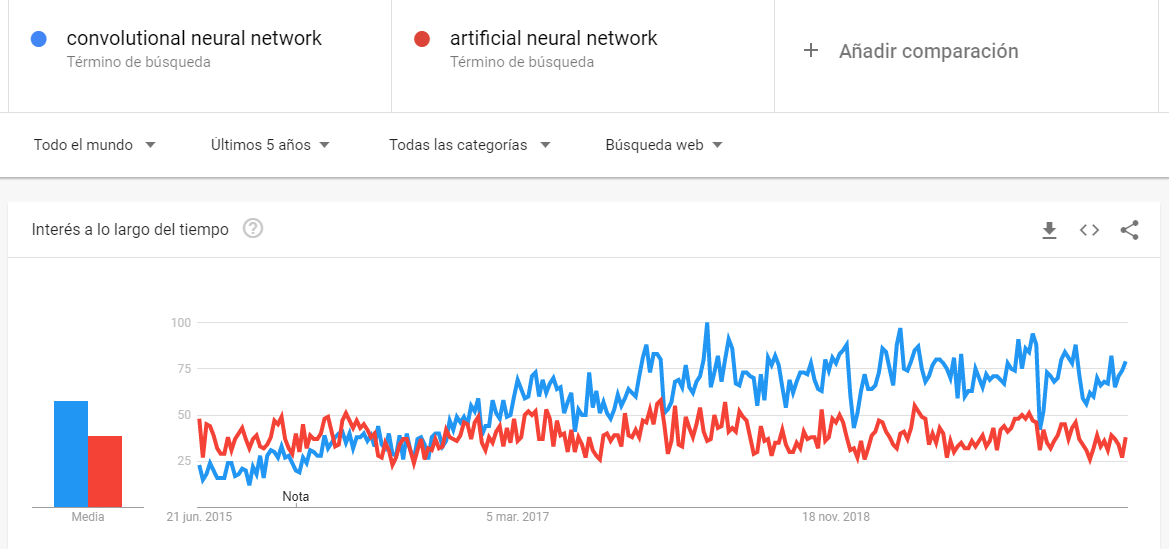
\includegraphics[keepaspectratio]{imagenes/capitulo1/busqueda_google.png}}

}

\caption{\label{fig-busqueda-google}búsqueda de términos de redes
neuronales en google trend}

\end{figure}%

Las \textbf{redes convolucionales} son actualmente utilizadas para
diferentes propósitos: tratamiento de imágenes(visión por computador,
extracción de características, segmentación, etc.), generación y
clasificación de texto(o audio), predicción de series temporales, etc.
En este capítulo veremos su aplicación en clasificación de imágenes y de
texto.

\subsection{Clasificación de
imágenes}\label{clasificaciuxf3n-de-imuxe1genes}

En este modelo de redes convolucionales las neuronas se corresponden a
campos receptivos similares a las neuronas en la corteza visual de un
cerebro humano. Este tipo de redes se han mostrado muy efectivas para
tareas de detección y categorización de objetos y en la clasificación y
segmentación de imágenes. Por ejemplo, estas redes en la década de 1990
las aplicó AT \& T para desarrollar un modelo para la lectura de
cheques. También más tarde se desarrollaron muchos sistemas OCR basados
en CNN. En esta arquitectura cada neurona de una capa no recibe
conexiones entrantes de todas las neuronas de la capa anterior, sino
sólo de algunas. Esta estrategia favorece que una neurona se especialice
en una región del conjunto de números (píxeles) de la capa anterior, lo
que disminuye notablemente el número de pesos y de operaciones a
realizar. Lo más normal es que neuronas consecutivas de una capa
intermedia se especialicen en regiones solapadas de la capa anterior.

Una forma intuitiva para entender cómo trabajan estas redes neuronales
es ver cómo nos representamos y vemos las imágenes. Para reconocer una
cara primero tenemos que tener una imagen interna de lo que es una cara.
Y a una imagen de una cara la reconocemos porque tiene nariz, boca,
orejas, ojos, etc. Pero en muchas ocasiones una oreja está tapada por el
pelo, es decir, los elementos de una cara se pueden ocultar de alguna
manera. Antes de clasificarla, tenemos que saber la proporción y
disposición y también cómo se relacionan la partes entre sí.

Para saber si las partes de la cara se encuentran en una imagen tenemos
que identificar previamente líneas bordes, formas, texturas, relación de
tamaño, etcétera. En una red convolucional, cada capa lo que va a ir
aprendiendo son los diferentes niveles de abstracción de la imagen
inicial. Para comprender mejor el concepto anterior hemos seleccionado
esta imagen de Raschka y Mirjalili (2019) donde se observa como partes
del perro se transforman en neuronas del mapa de características

\begin{figure}

\centering{

\pandocbounded{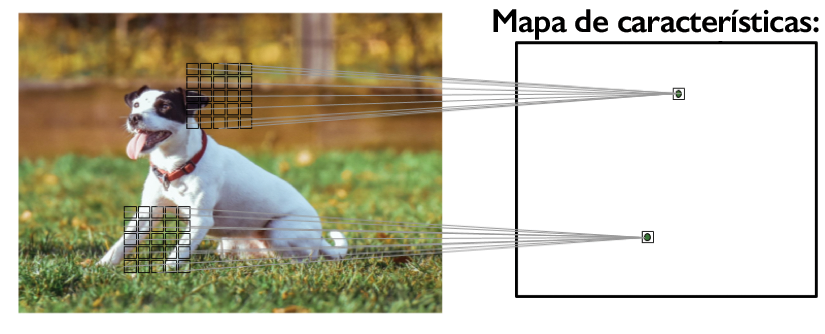
\includegraphics[keepaspectratio]{imagenes/capitulo1/correspondencia_featrures.png}}

}

\caption{\label{fig-correspondencia-features}Correspondencia de zonas de
la imagen y mapa de características}

\end{figure}%

El objetivo de las redes CNN es aprender características de orden
superior utilizando la operación de convolución.

Puesto que las redes neuronales convolucionales pueden aprender
relaciones de entrada-salida (donde la entrada es una imagen en este
caso), en la convolución, cada pixel de salida es una combinación lineal
de los pixeles de entrada.

La \textbf{convolución} consiste en \textbf{filtrar} una imagen
utilizando una \textbf{máscara}. Diferentes máscaras producen distintos
resultados. Las máscaras representan las conexiones entre neuronas de
capas anteriores. Estas capas aprenden progresivamente las
características de orden superior de la entrada sin procesar.

Las redes neuronales convolucionales se forman usando dos tipos de
capas: convolucionales y pooling. La capa de convolución transforma los
datos de entrada a través de una operación matemática llamada
convolución. Esta operación describe cómo fusionar dos conjuntos de
información diferentes. A esta operación se le suele aplicar una función
de transformación, generalmente la RELU. Después de la capa o capas de
convolución se usa una capa de pooling, cuya función es resumir las
respuestas de las salidas cercanas. Antes de obtener el output unimos la
última capa de pooling con una red densamente conectada. Previamente se
ha aplanado (Flatering) la última capa de pooling para obtener un vector
de entrada a la red neural final que nos ofrecerá los resultados.

\begin{figure}

\centering{

\pandocbounded{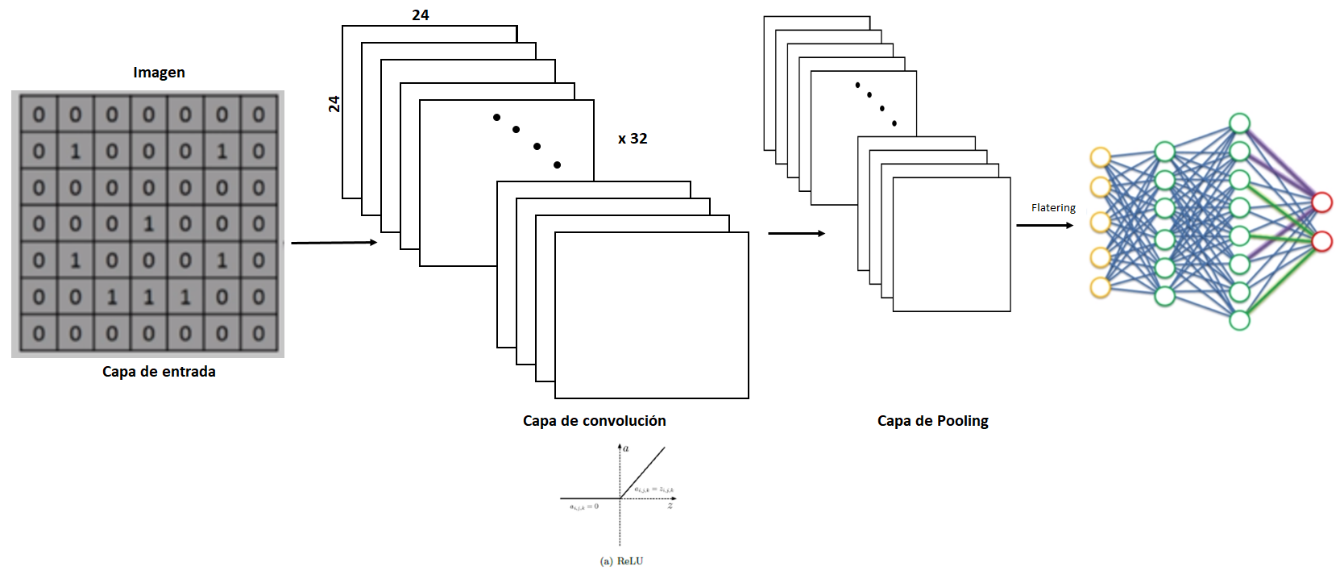
\includegraphics[keepaspectratio]{imagenes/capitulo1/arquitectura_convolucional.png}}

}

\caption{\label{fig-arquitectura_convolucional}Arquitectura de una CNN}

\end{figure}%

Las redes neuronales convolucionales debido a su forma de concebirse son
aptas para poder aprender a clasificar todo tipo de datos donde éstos
estén distribuidos de una forma continua a lo largo del mapa de entrada,
y a su vez sean estadísticamente similares en cualquier lugar del mapa
de entrada. Por esta razón, son especialmente eficaces para clasificar
imágenes. También pueden ser aplicadas para la clasificación de series
de tiempo o señales de audio.

En relación con el color y la forma de codificarse, en las redes
convolucionales se realiza en tensores 3D, dos ejes para el ancho
(width) y el alto (height) y el otro eje llamado de profundidad (depht)
que es el canal del color con valor tres si trabajamos con imágenes de
color RGB (Red, Green y Blue) rojo, verde y azul. Si disponemos de
imágenes en escala de grises el valor de depht es uno. La base de datos
MNIST (National Institute of Standards and Technology database) con la
que trabajaremos en este epígrafe contiene imágenes de 28 x 28 pixeles,
los valores de height y de widht son ambos 28, y al ser una base de
datos en blanco y negro el valor de depht es 1.

Las imágenes son matrices de píxeles que van de cero a 255 y que para la
red neuronal se normalizan para que sus valores oscilen entre cero y
uno.

\subsubsection{Convolución}\label{convoluciuxf3n}

En las redes convolucionales todas las neuronas de la capa de entrada
(los píxeles de las imágenes) no se conectan con todas las neuronas de
la capa oculta del primer nivel como lo hacen las redes clásicas del
tipo perceptrón multicapa o las redes que conocemos de forma genérica
como redes densamente conectadas. Las conexiones se realizan por
pequeñas zonas de la capa de entrada.

\begin{figure}

\centering{

\pandocbounded{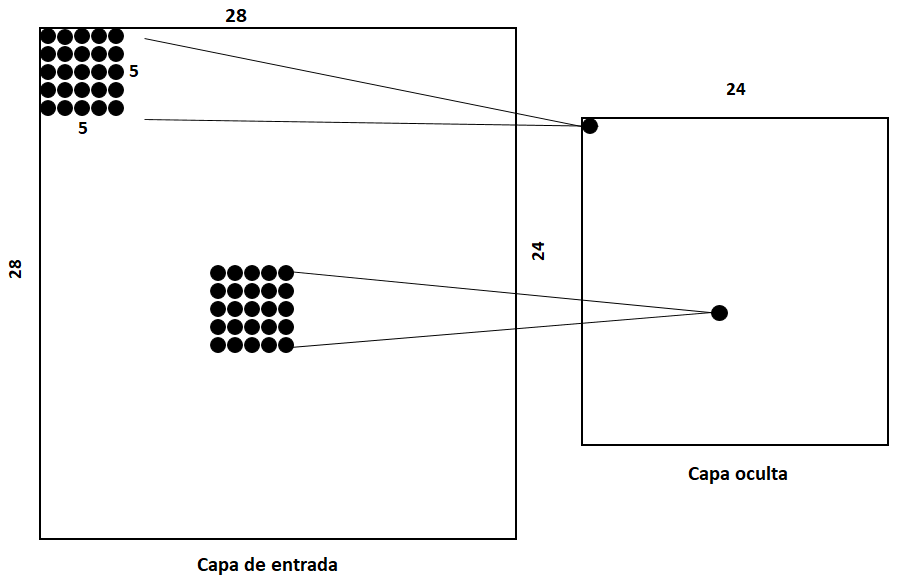
\includegraphics[keepaspectratio]{imagenes/capitulo1/conexion_neuronas_convolucional.png}}

}

\caption{\label{fig-conexion-neuronas-convolucional}Conexión de las
neuronas de la capa de entrada con la capa oculta}

\end{figure}%

Veamos un ejemplo para la base de datos de los dígitos del 1 a 9. Vamos
a conectar cada neurona de la capa oculta con una región de 5 x 5
neurona, es decir, con 25 neuronas de la capa de entrada, que podemos
denominarla ventana. Esta ventana va a ir recorriendo todo el espacio de
entrada de 28 x 28 empezando por arriba y desplazándose de izquierda a
derecha y de arriba abajo. Suponemos que los desplazamientos de la
ventana son de un paso (un pixel) aunque este es un parámetro de la red
que podemos modificar (en la programación lo llamaremos stride).

Para conectar la capa de entrada con la de salida utilizaremos una
matriz de pesos (W) de tamaño 3 x 3 que recibe el nombre de filtro
(filter) y el valor del sesgo. Para obtener el valor de cada neurona de
la capa oculta realizaremos el producto escalar entre el filtro y la
ventana de la capa de entrada. Utilizamos el mismo filtro para obtener
todas las neuronas de la capa oculta, es decir en todos los productos
escalares siempre utilizamos la misma matriz, el mismo filtro.

Se definen matemáticamente estos productos escalares a través de la
siguiente expresión:

\[
Y=X * W \rightarrow Y[i, j]=\sum_{k_1=-\infty}^{+\infty} \sum_{k_2=-\infty}^{+\infty} X\left[i-k_1, j-k_2\right] W\left[k_1, k_2\right]
\]

\begin{figure}

\centering{

\pandocbounded{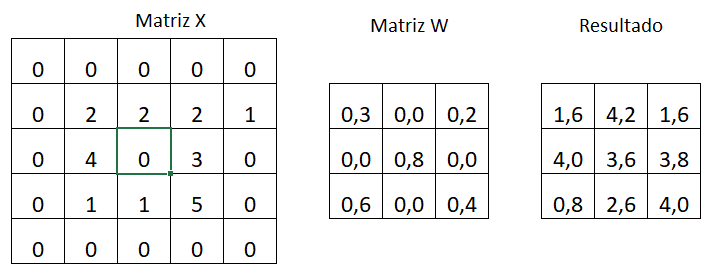
\includegraphics[keepaspectratio]{imagenes/capitulo1/producto_convolucion.png}}

}

\caption{\label{fig-producto_convolucion}Convolución}

\end{figure}%

Como en este tipo de red un filtro sólo nos permite revelar una
característica muy concreta de la imagen, lo que se propone es usar
varios filtros simultáneamente, uno para cada característica que
queramos detectar. Una forma visual de representarlo (si suponemos que
queremos aplicar 32 filtros) es como se muestra a continuación:

\begin{figure}

\centering{

\pandocbounded{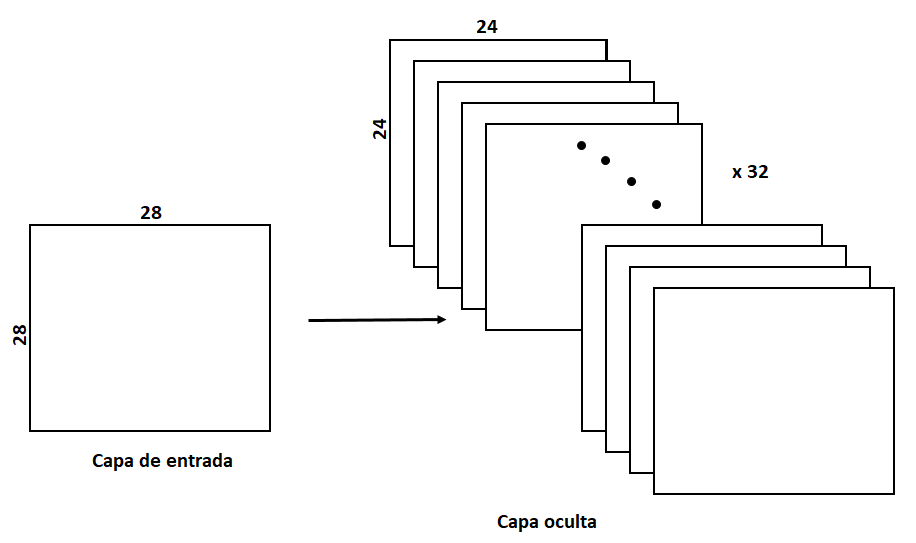
\includegraphics[keepaspectratio]{imagenes/capitulo1/primera_capa_convolucional.png}}

}

\caption{\label{fig-primera-capa-convolucional}Primera capa de la red
convolucional con 32 filtros}

\end{figure}%

Al resultado de la aplicación de los diferentes filtros se les suele
aplicar la función de activación denominada RELU y que ya se comentó en
la introducción.

Una interesante fuente de información es la documentación del software
gratuito GIMP donde expone diferentes efectos que se producen en las
imágenes al aplicar diversas convoluciones.

Un ejmplo claro y didáctico lo podemos obtener de la docuemntación del
software libre de dibujo y tratamiento de imágenes denominado GIMP
(https://docs.gimp.org/2.6/es/plug-in-convmatrix.html). Algunos de estos
efectos nos ayudan a entender la operación de los filtros en las redes
convolucionales y cómo afectan a las imágenes, en concreto, el ejemplo
que presenta lo realiza sobre la figura del Taj Mahal.

El filtro enfocar lo que consigue es afinar los rasgos, los contornos lo
que nos permite agudizar los objetos de la imagen. Toma el valor central
de la matriz de cinco por cinco lo multiplica por cinco y le resta el
valor de los cuatro vecinos. Al final hace una media, lo que mejora la
resolución del pixel central porque elimina el ruido o perturbaciones
que tiene de sus pixeles vecinos.

\textbf{El filtro enfocar (Sharpen)}

\begin{figure}

\centering{

\pandocbounded{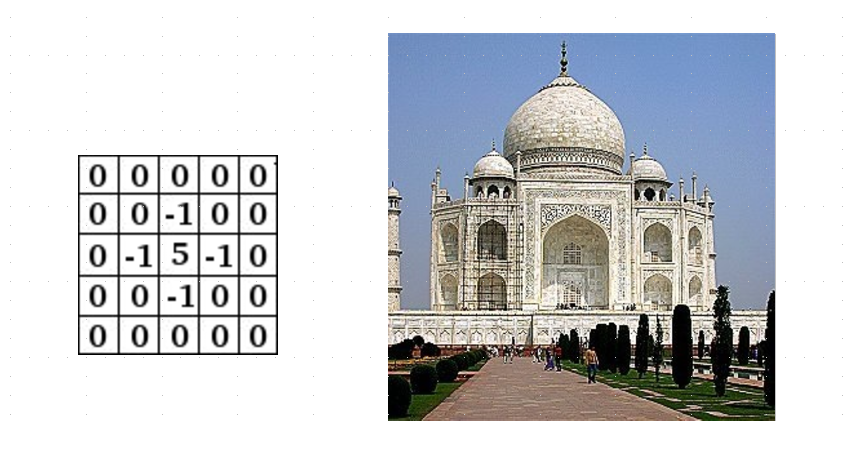
\includegraphics[keepaspectratio]{imagenes/capitulo1/filtro_enfocar.png}}

}

\caption{\label{fig-filtro_enfocar}Filtro Enfocar}

\end{figure}%

Lo contario al filtro enfocar lo obtenemos a través de la matriz
siguiente, difuminando la imagen al ser estos píxeles mezclados o
combinados con los pixeles cercanos. Promedia todos los píxeles vecinos
a un pixel dado lo que implica que se obtienen bordes borrosos.

\textbf{Filtro desenfocar}

\begin{figure}

\centering{

\pandocbounded{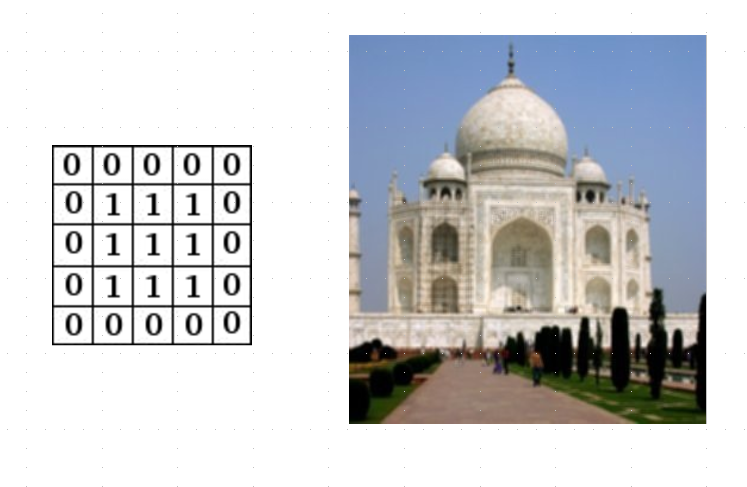
\includegraphics[keepaspectratio]{imagenes/capitulo1/filtro_desenfocar.png}}

}

\caption{\label{fig-filtro_desenfocar}Filtro DesEnfocar}

\end{figure}%

\textbf{Filtro Detectar bordes (Edge Detect)}

Este efecto se consigue mejorando los límites o las aristas de la
imagen. En cada píxel se elimina su vecino inmediatamente anterior en
horizontal y en vertical. Se eliminan las similitudes vecinas y quedan
los bordes resaltados. Al pixel central se le suman los cuatro píxeles
vecinos y lo que queda al final es una medida de cómo de diferente es un
píxel frente a sus vecinos. En el ejemplo, al hacer esto da un valor de
cero de ahí que se observen tantas zonas oscuras.

\begin{figure}

\centering{

\pandocbounded{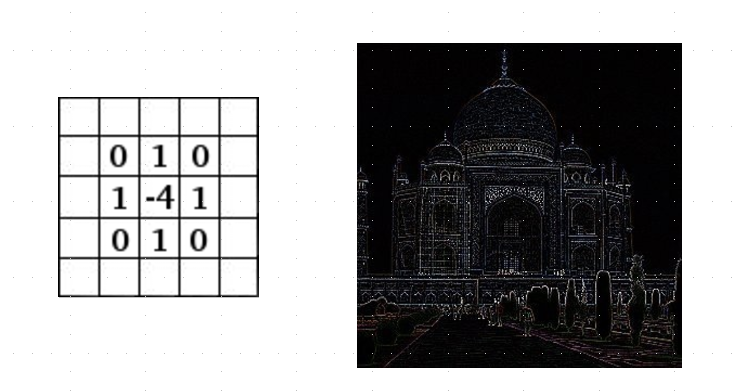
\includegraphics[keepaspectratio]{imagenes/capitulo1/filtro_bordes.png}}

}

\caption{\label{fig-filtro_bordes}Filtro Detectar Bordes}

\end{figure}%

\textbf{Filtro Repujado (Emboss)}

En este filto se observa que la matriz es simétrica y lo que intenta a
través del diseño del filtro es mejorar los píxeles centrales y de
derecha abajo restándole los anteriores. Se obtiene lo que en fotografía
se conoce como un claro oscuro. Trata de mejorar las partes que tienen
mayor relevancia.

\begin{figure}

\centering{

\pandocbounded{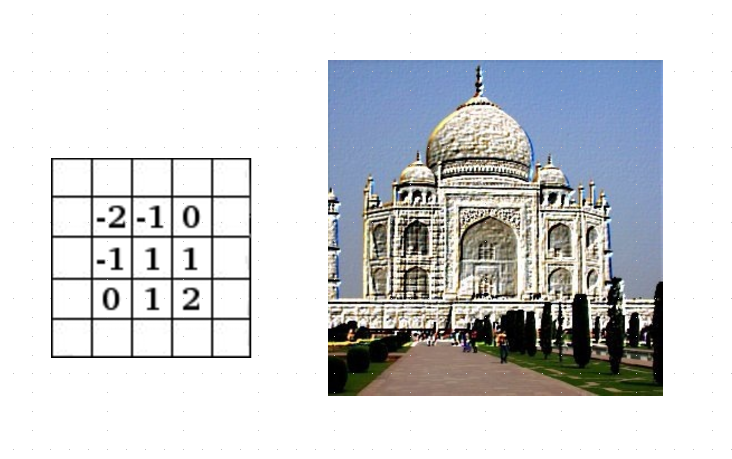
\includegraphics[keepaspectratio]{imagenes/capitulo1/filtro_emboss.png}}

}

\caption{\label{fig-filtro_emboss}Filtro Emboss}

\end{figure}%

\subsubsection{Pooling}\label{pooling}

Con la operación de \textbf{pooling} se trata de condensar la
información de la capa convolucional. A este procedimiento también se le
conoce como \textbf{submuestreo}.

Es simplemente una operación en la que reducimos los parámetros de la
red. Se aplica normalmente a través de dos operaciones:
\textbf{max-pooling} y \textbf{mean-pooling}, que también es conocido
como average-pooling. Tal y como se observa en la imagen siguiente,
desde la capa de convolución se genera una nueva capa aplicando la
operación a todas las agrupaciones, donde previamente hemos elegido el
tamaño de la región; en la figura siguiente es de tamaño 2, con lo que
pasamos de un espacio de 24 x 24 neuronas a la mitad, 12 x 12 en la capa
de pooling.

\begin{figure}

\centering{

\pandocbounded{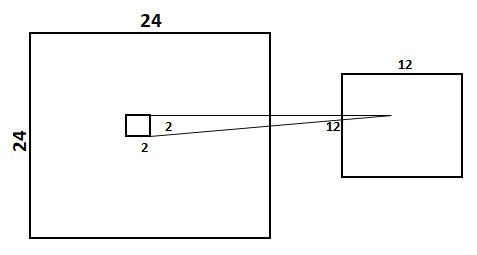
\includegraphics[keepaspectratio]{imagenes/capitulo1/pooling.png}}

}

\caption{\label{fig-pooling}Etapa de pooling de tamaño 2 x 2}

\end{figure}%

Vamos a estudiar el pooling suponiendo que tenemos una imagen de 5 x 5
píxeles y que queremos efectuar una agrupación max-pooling. Es la más
utilizada, ya que obtiene buenos resultados. Observamos los valores de
la matriz y se escoge el valor máximo de los cuatro bloques de matrices
de dos por dos. Max Pooling

En la agrupación Average Pooling la operación que se realiza es
sustituir los valores de cada grupo de entrada por su valor medio. Esta
transformación es menos utilizada que el max-pooling.

La transformación max-pooling presenta un tipo de invarianza local:
pequeños cambios en una región local no varían el resultado final
realizado con el max -- pooling: se mantiene la relación espacial. Para
ilustrar este concepto hemos escogido la imagen que presenta Torres
(2020) donde se ilustra como partiendo de una matriz de 12 x 12 que
representa al número 7, al aplicar la operación de max-pooling con una
ventana de 2 x 2 se conserva la relación espacial.

\begin{figure}

\centering{

\pandocbounded{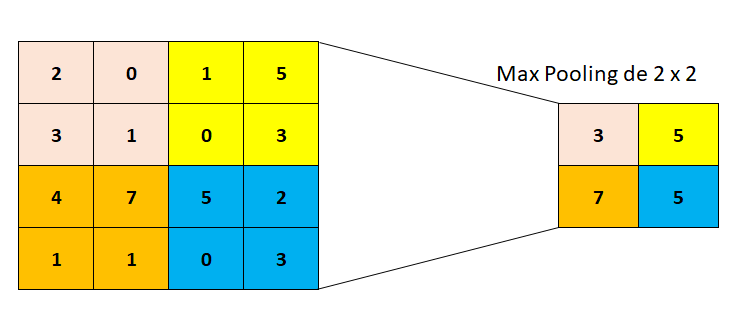
\includegraphics[keepaspectratio]{imagenes/capitulo1/max_pooling.png}}

}

\caption{\label{fig-max-pooling}Max Pooling}

\end{figure}%

\begin{figure}

\centering{

\pandocbounded{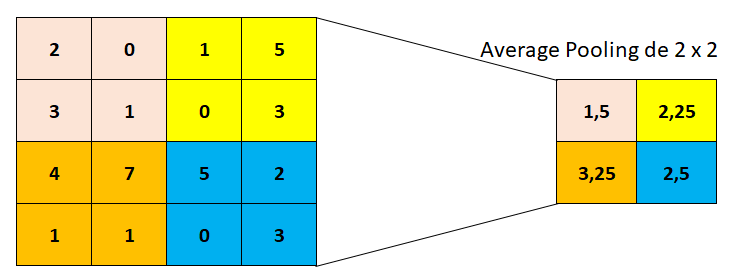
\includegraphics[keepaspectratio]{imagenes/capitulo1/average_pooling.png}}

}

\caption{\label{fig-average-pooling}Average Pooling}

\end{figure}%

\begin{figure}

\centering{

\pandocbounded{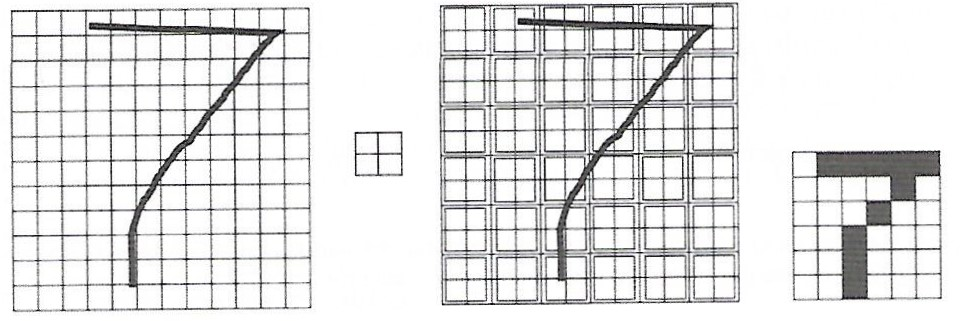
\includegraphics[keepaspectratio]{imagenes/capitulo1/transformacion_pooling.png}}

}

\caption{\label{fig-transformacion-pooling}Mantenimiento del pooling con
la transformación}

\end{figure}%

\subsubsection{Padding}\label{padding}

Para explicar el concepto del \textbf{Padding} vamos a suponer que
tenemos una imagen de 5 x 5 píxeles, es decir 25 neuronas en la capa de
entrada, y que elegimos, para realizar la convolución, una ventana de 3
x 3. El número de neuronas de la capa oculta resultará ser de nueve.
Enumeramos los píxeles de la imagen de forma natural del 1 al 25 para
que resulte más sencillo de entender.

\begin{figure}

\centering{

\pandocbounded{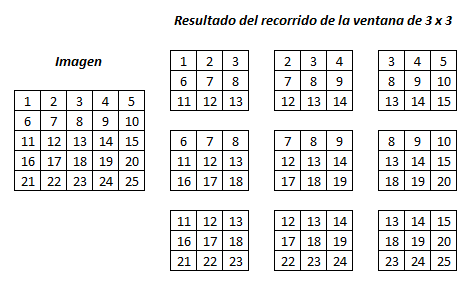
\includegraphics[keepaspectratio]{imagenes/capitulo1/sin_padding.png}}

}

\caption{\label{fig-sin-padding}Operación de convolución con una ventana
de 3 x 3}

\end{figure}%

Pero si queremos obtener un tensor de salida que tenga las mismas
dimensiones que la entrada podemos rellenar la matriz de ceros antes de
deslizar la ventana por ella. Vemos la figura siguiente donde ya se ha
rellenado de valores cero y obtenemos, después de deslizar la ventana de
3 x3 de izquierda a derecha y de arriba abajo, las veinticinco matrices
de la figura nº 71

\begin{figure}

\centering{

\pandocbounded{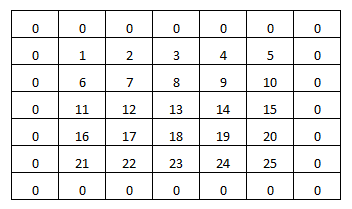
\includegraphics[keepaspectratio]{imagenes/capitulo1/relleno_ceros.png}}

}

\caption{\label{fig-relleno-ceros}Imagen con relleno de ceros}

\end{figure}%

\begin{figure}

\centering{

\pandocbounded{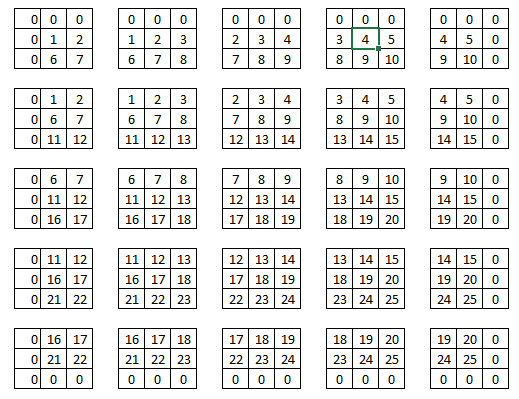
\includegraphics[keepaspectratio]{imagenes/capitulo1/con_padding.png}}

}

\caption{\label{fig-con-padding}Operación de convolución con ventana 3 x
3 y padding}

\end{figure}%

\subsubsection{Stride}\label{stride}

Hasta ahora, la forma de recorrer la matriz a través de la ventana se
realiza desplazándola de \textbf{un solo paso}, pero podemos cambiar
este hiperparámetro conocido como \textbf{stride}. Al aumentar el paso
se decrementa la información que pasará a la capa posterior. A
continuación, se muestra el resultado de las cuatro matrices que
obtenemos con un stride de valor 3.

\begin{figure}

\centering{

\pandocbounded{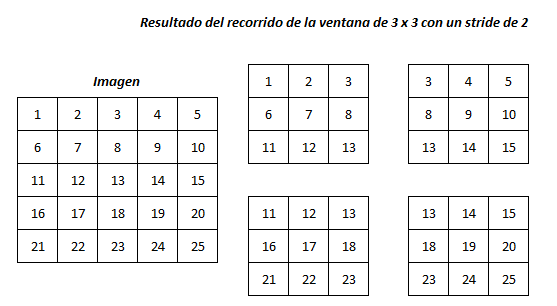
\includegraphics[keepaspectratio]{imagenes/capitulo1/con_stride2.png}}

}

\caption{\label{fig-con-stride2}Operación de convolución con una ventana
de 3 x 3 y stride 2}

\end{figure}%

Finalmente, para resumir, una \textbf{red convolucional} contiene los
siguientes elementos:

\begin{itemize}
\tightlist
\item
  \textbf{Entrada}: Son el número de pixeles de la imagen. Serán alto,
  ancho y profundidad. Tenemos un solo color (escala de grises) o tres:
  rojo, verde y azul.
\item
  \textbf{Capa de convolución}: procesará la salida de neuronas que
  están conectadas en «regiones locales» de entrada (es decir pixeles
  cercanos), calculando el producto escalar entre sus pesos (valor de
  pixel) y una pequeña región a la que están conectados. En este
  epígrafe se presentan las imágenes con 32 filtros, pero puede
  realizarse con la cantidad que deseemos.
\item
  \textbf{Capa RELU} Se aplicará la función de activación en los
  elementos de la matriz.
\item
  \textbf{Pooling} (agrupar) o Submuestreo: Se procede normalmente a una
  reducción en las dimensiones alto y ancho, pero se mantiene la
  profundidad.
\item
  \textbf{Capa tradicional}. Se finalizará con la red de neuronas
  feedforward (Perceptrón multicapa que se denomina normalmente como red
  densamente conectada) que vinculará con la última capa de subsampling
  y finalizará con la cantidad de neuronas que queremos clasificar. En
  el gráfico siguiente se muestran todas las fases de una red neuronal
  convolucional.
\end{itemize}

\begin{figure}

\centering{

\pandocbounded{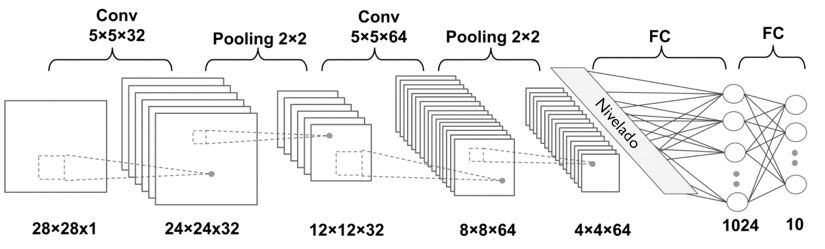
\includegraphics[keepaspectratio]{imagenes/capitulo1/convolucion_completa.png}}

}

\caption{\label{fig-convolucion-completa}Operación de convolución
completa}

\end{figure}%

\subsubsection{Redes convolucionales con nombre
propio}\label{redes-convolucionales-con-nombre-propio}

Existen en la actualidad muchas arquitecturas de redes neuronales
convolucionales que ya están preparadas, probadas, disponibles e
incorporadas en el software de muchos programas como Keras y Tensorflow.

Vamos a comentar algunos de estos modelos, bien por ser los primeros, o
por sus excelentes resultados en concursos como el ILSVRC (Large Scale
Visual Recognition Challenge).

Estas estructuras merecen atención dado que son excelentes para
estudiarlas e incorporarlas por su notable éxito. El ILSVRC fue un
concurso celebrado de 2011 a 2016 de donde nacieron las principales
aportaciones efectuadas en las redes convolucionales. Este concurso fue
diseñado para estimular la innovación en el campo de la visión
computacional. Actualmente se desarrollan este tipo de concursos a
través de la plataforma web: https://www.kaggle.com/ Para ver más
prototipos de redes convolucionales y los últimos avances y consejos
sobre las redes convolucionales se puede consultar el siguiente artículo
``Recent Advances in Convolutional Neural Networks'' de Jiuxiang. G. et
al.~(2019)

Los cinco modelos más destacados hasta el año 2017 son los siguientes:
LeNet-5, Alexnet, GoogLeNet, VGG y Restnet.

\begin{itemize}
\item
  \textbf{LeNet-5}. Este modelo de Yann LeCun de los años 90 consiguió
  excelentes resultados en la lectura de códigos postales consta de
  imágenes de entrada de 32 x 32 píxeles seguida de dos etapas de
  convolución -- pooling, una capa densamente conectada y una capa
  softmax final que nos permite conocer los números o las imágenes.
\item
  \textbf{AlexNet}. Fue la arquitectura estrella a partir del año 2010
  en el ILSVRC y popularizada en el documento de 2012 de Alex
  Krizhevsky, et al.~titulado''Clasificación de ImageNet con redes
  neuronales convolucionales profundas''. Podemos resumir los aspectos
  clave de la arquitectura relevantes en los modelos modernos de la
  siguiente manera: • Empleo de la función de activación ReLU después de
  capas convolucionales y softmax para la capa de salida. • Uso de la
  agrupación máxima en lugar de la agrupación media. • Utilización de la
  regularización de Dropout entre las capas totalmente conectadas. •
  Patrón de capa convolucional alimentada directamente a otra capa
  convolucional. • Uso del aumento de datos (Data Aumentation,)
\item
  \textbf{VGG}. Este prototipo fue desarrollado por un grupo de
  investigación de Geometría Visual en Oxford. Obtuvo el segundo puesto
  en la competición del año 2014 del ILSVRC. Las aportaciones
  principales de la investigación se pueden encontrar en el documento
  titulado ``~Redes convolucionales muy profundas para el reconocimiento
  de imágenes a gran escala~'' desarrollado por Karen Simonyan y Andrew
  Zisserman. Este modelo contribuyó a demostrar que la profundidad de la
  red es una componente crítica para alcanzar unos buenos resultados.
  Otra diferencia importante con los modelos anteriores y que
  actualmente es muy utilizada es el uso de un gran número de filtros y
  de tamaño reducido. Estas redes emplean ejemplos de dos, tres e
  incluso cuatro capas convolucionales apiladas antes de usar una capa
  de agrupación máxima. En esta arquitectura el número de filtros
  aumenta con la profundidad del modelo. El modelo comienza con 64 y
  aumenta a través de los filtros de 128, 256 y 512 al final de la parte
  de extracción de características del modelo. Los investigadores
  evaluaron varias variantes de la arquitectura si bien en los programas
  sólo se hace referencia a dos de ellas que son las que aportan un
  mayor rendimiento y que son nombradas por las capas que tienen: VGG-16
  y VGG-19.
\item
  \textbf{GoogLeNet}. GoogLeNet fue desarrolado por investigadores de
  Google Research. de Google, que con su módulo denominado de inception
  reduce drásticamente los parámetros de la red (10 veces menos que
  AlexNet) y de ella han derivado varias versiones como la Inception-v4.
  Esta arquitectura ganó la competición en el año 2014 y su éxito se
  debió a que la red era mucho más profunda (muchas más capas) y como ya
  se ha indicado introdujeron en el modelo las subredes llamadas
  inception. Las aportaciones principales en el uso de capas
  convolucionales fueron propuestos en el documento de 2015 por
  Christian Szegedy, et al.~titulado ``~Profundizando con las
  convoluciones~''. Estos autores introducen una arquitectura llamada
  ``inicio'' y un modelo específico denominado GoogLenet. El módulo
  inicio es un bloque de capas convolucionales paralelas con filtros de
  diferentes tamaños y una capa de agrupación máxima de 3 × 3, cuyos
  resultados se concatenan. Otra decisión de diseño fundamental en el
  modelo inicial fue la conexión de la salida en diferentes puntos del
  modelo que lograron realizar con la creación de pequeñas redes de
  salida desde la red principal y que fueron entrenadas para hacer una
  predicción. La intención era proporcionar una señal de error adicional
  de la tarea de clasificación en diferentes puntos del modelo profundo
  para abordar el problema de los gradientes de fuga.
\item
  \textbf{Red Residual o ResNet}. Esta arquitectura gano la competición
  de 2015 y fue creada por el grupo de investigación de Microsoft. Se
  puede ampliar la información en He, et al.~en su documento de 2016
  titulado ``~Aprendizaje profundo residual para el reconocimiento de la
  imagen~''. Esta red es extremadamente profunda con 152 capas,
  confirmando al pasar los años que las redes son cada vez más
  profundas, más capas, pero con menos parámetros que estimar. La
  cuestión clave del diseño de esta red es la incorporación de la idea
  de bloques residuales que hacen uso de conexiones directa. Un bloque
  residual, según los autores, ``es un patrón de dos capas
  convolucionales con activación ReLU donde la salida del bloque se
  combina con la entrada al bloque, por ejemplo, la conexión de acceso
  directo'' Otra clave, en este caso para el entrenamiento de la red tan
  profunda es lo que llamaron skip connections que implica que la señal
  con la que se alimenta una capa también se agregue a una capa que se
  encuentre más adelante. Resumiendo, las tres principales aportaciones
  de este modelo son:

  \begin{itemize}
  \tightlist
  \item
    Empleo de conexiones de acceso directo.
  \item
    Desarrollo y repetición de los bloques residuales.
  \item
    Modelos muy profundos (152 capas) Aunque se encuentran otros modelos
    que también son muy populares con 34, 50 y 101 capas.
  \end{itemize}
\end{itemize}

Una buena parte de los modelos comentados se incluyen en la librería de
Keras y se pueden encontrar en la siguiente dirección de internet:
https://keras.io/api/applications/ Según los autores del programa Keras:
``Las aplicaciones Keras son modelos de aprendizaje profundo que están
disponibles junto con pesos preentrenados. Estos modelos se pueden usar
para predicción, extracción de características y ajustes. Los pesos se
descargan automáticamente cuando se crea una instancia de un modelo. Se
almacenan en \textasciitilde{} / .keras / models /. Tras la creación de
instancias, los modelos se construirán de acuerdo con el formato de
datos de imagen establecido en su archivo de configuración de Keras en
\textasciitilde{} / .keras / keras.json. Por ejemplo, si ha configurado
image\_data\_format = channel\_last, cualquier modelo cargado desde este
repositorio se construirá de acuerdo con la convención de formato de
datos TensorFlow,''Altura-Ancho-Profundidad''.

\begin{figure}

\centering{

\pandocbounded{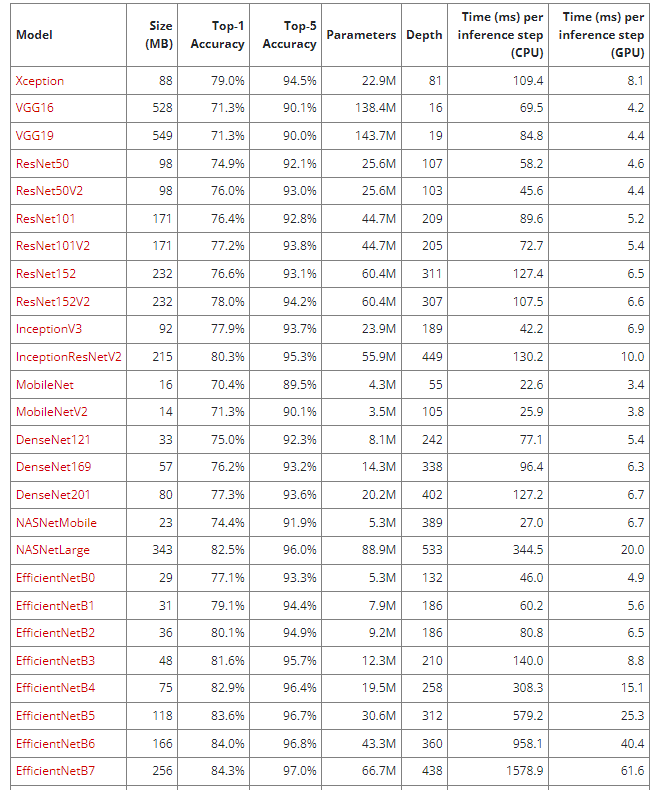
\includegraphics[keepaspectratio]{imagenes/capitulo1/modelos_entrenados.png}}

}

\caption{\label{fig-modelos-entrenados}Modelos preentrenados en Keras}

\end{figure}%

\subsubsection{Ejemplos de Redes Convolucionales con
keras}\label{ejemplos-de-redes-convolucionales-con-keras}

\textbf{Red Convolucional con imágenes importadas a memoria}

En este ejemplo vamos a usar imágenes que vienen preparadas dentro de un
array de datos que se carga directamente en memoria.

\begin{Shaded}
\begin{Highlighting}[numbers=left,,]

\CommentTok{\# Importamos las librerías de keras/tensorflow}
\ImportTok{from}\NormalTok{ tensorflow }\ImportTok{import}\NormalTok{ keras}
\ImportTok{from}\NormalTok{ tensorflow.keras }\ImportTok{import}\NormalTok{ layers}

\CommentTok{\# Importamos la librería de los datasets de keras y cogemos el de mnist}
\ImportTok{from}\NormalTok{ tensorflow.keras.datasets }\ImportTok{import}\NormalTok{ mnist}

\CommentTok{\# Obtenemos los datos de entrenamiento y test}
\CommentTok{\# separados en las imagenes y las etiquetas de las mismas}
\NormalTok{(train\_images, train\_labels), (test\_images, test\_labels) }\OperatorTok{=}\NormalTok{ mnist.load\_data()}

\CommentTok{\# Reestructuramos los datos de las imágenes para que se traten como imagen}
\NormalTok{train\_images }\OperatorTok{=}\NormalTok{ train\_images.reshape((}\DecValTok{60000}\NormalTok{, }\DecValTok{28}\NormalTok{, }\DecValTok{28}\NormalTok{, }\DecValTok{1}\NormalTok{))}
\CommentTok{\# Dividimos entre 255 para "normalizar" el dato y dejarlo entre 0 y 1}
\NormalTok{train\_images }\OperatorTok{=}\NormalTok{ train\_images.astype(}\StringTok{"float32"}\NormalTok{) }\OperatorTok{/} \DecValTok{255}
\CommentTok{\# Reestructuramos los datos de las imágenes para que se traten como imagen}
\NormalTok{test\_images }\OperatorTok{=}\NormalTok{ test\_images.reshape((}\DecValTok{10000}\NormalTok{, }\DecValTok{28}\NormalTok{, }\DecValTok{28}\NormalTok{, }\DecValTok{1}\NormalTok{))}
\CommentTok{\# Dividimos entre 255 para "normalizar" el dato y dejarlo entre 0 y 1}
\NormalTok{test\_images }\OperatorTok{=}\NormalTok{ test\_images.astype(}\StringTok{"float32"}\NormalTok{) }\OperatorTok{/} \DecValTok{255}


\CommentTok{\# Creamos el modelo}
\CommentTok{\# Capa de entrada formato 28x28 pixels y sólo un canal de color (escala de grises}
\NormalTok{inputs }\OperatorTok{=}\NormalTok{ keras.Input(shape}\OperatorTok{=}\NormalTok{(}\DecValTok{28}\NormalTok{, }\DecValTok{28}\NormalTok{, }\DecValTok{1}\NormalTok{))}

\CommentTok{\# Añadimos capa de convolución con 32 filtros de tamaño 3 y activación relu}
\NormalTok{x }\OperatorTok{=}\NormalTok{ layers.Conv2D(filters}\OperatorTok{=}\DecValTok{32}\NormalTok{, kernel\_size}\OperatorTok{=}\DecValTok{3}\NormalTok{, activation}\OperatorTok{=}\StringTok{"relu"}\NormalTok{)(inputs)}
\CommentTok{\# Añadimos capa de pooling, tipo max y de tamaño 2}
\NormalTok{x }\OperatorTok{=}\NormalTok{ layers.MaxPooling2D(pool\_size}\OperatorTok{=}\DecValTok{2}\NormalTok{)(x)}
\CommentTok{\# Añadimos capa de convolución con 64 filtros de tamaño 3 y activación relu}
\NormalTok{x }\OperatorTok{=}\NormalTok{ layers.Conv2D(filters}\OperatorTok{=}\DecValTok{64}\NormalTok{, kernel\_size}\OperatorTok{=}\DecValTok{3}\NormalTok{, activation}\OperatorTok{=}\StringTok{"relu"}\NormalTok{)(x)}
\CommentTok{\# Añadimos capa de pooling, tipo max y de tamaño 2}
\NormalTok{x }\OperatorTok{=}\NormalTok{ layers.MaxPooling2D(pool\_size}\OperatorTok{=}\DecValTok{2}\NormalTok{)(x)}
\CommentTok{\# Añadimos capa de convolución con 128 filtros de tamaño 3 y activación relu}
\NormalTok{x }\OperatorTok{=}\NormalTok{ layers.Conv2D(filters}\OperatorTok{=}\DecValTok{128}\NormalTok{, kernel\_size}\OperatorTok{=}\DecValTok{3}\NormalTok{, activation}\OperatorTok{=}\StringTok{"relu"}\NormalTok{)(x)}

\CommentTok{\# Aplanamos los datos}
\NormalTok{x }\OperatorTok{=}\NormalTok{ layers.Flatten()(x)}

\CommentTok{\# Ponemos una capa densamente conectada}
\NormalTok{x }\OperatorTok{=}\NormalTok{ layers.Dense(}\DecValTok{512}\NormalTok{, activation}\OperatorTok{=}\StringTok{"relu"}\NormalTok{)(x)}

\CommentTok{\# La salida la hacemos de tipo softmax con 10 neuronas (números de clases diferentes)}
\NormalTok{outputs }\OperatorTok{=}\NormalTok{ layers.Dense(}\DecValTok{10}\NormalTok{, activation}\OperatorTok{=}\StringTok{"softmax"}\NormalTok{)(x)}

\CommentTok{\# Construimos el modelo de la Red Neuronal Convolucional}
\NormalTok{model }\OperatorTok{=}\NormalTok{ keras.Model(inputs}\OperatorTok{=}\NormalTok{inputs, outputs}\OperatorTok{=}\NormalTok{outputs)}

\CommentTok{\# Mostramos el Modelo creado}
\NormalTok{model.summary()}

\CommentTok{\# Compilamos el modelo definiendo el optimizador, función de pérdida y métrica}
\CommentTok{\# RMSProp, sparse\_categorical\_crossentropy, accuracy}
\NormalTok{model.}\BuiltInTok{compile}\NormalTok{(optimizer}\OperatorTok{=}\StringTok{"rmsprop"}\NormalTok{,}
\NormalTok{    loss}\OperatorTok{=}\StringTok{"sparse\_categorical\_crossentropy"}\NormalTok{,}
\NormalTok{    metrics}\OperatorTok{=}\NormalTok{[}\StringTok{"accuracy"}\NormalTok{])}

\CommentTok{\# Realizamos el entrenamiento}
\CommentTok{\# 5 épocos (iteraciones), con tamaño de batch de 64}
\NormalTok{history }\OperatorTok{=}\NormalTok{ model.fit(train\_images, train\_labels, epochs}\OperatorTok{=}\DecValTok{5}\NormalTok{, batch\_size}\OperatorTok{=}\DecValTok{64}\NormalTok{)}


\CommentTok{\# summarize history for accuracy}
\NormalTok{plt.plot(history.history[}\StringTok{\textquotesingle{}accuracy\textquotesingle{}}\NormalTok{])}
\NormalTok{plt.title(}\StringTok{\textquotesingle{}model accuracy\textquotesingle{}}\NormalTok{)}
\NormalTok{plt.ylabel(}\StringTok{\textquotesingle{}accuracy\textquotesingle{}}\NormalTok{)}
\NormalTok{plt.xlabel(}\StringTok{\textquotesingle{}epoch\textquotesingle{}}\NormalTok{)}
\NormalTok{plt.legend([}\StringTok{\textquotesingle{}train\textquotesingle{}}\NormalTok{], loc}\OperatorTok{=}\StringTok{\textquotesingle{}upper left\textquotesingle{}}\NormalTok{)}
\NormalTok{plt.show()}

\CommentTok{\# summarize history for loss}
\NormalTok{plt.plot(history.history[}\StringTok{\textquotesingle{}loss\textquotesingle{}}\NormalTok{])}
\NormalTok{plt.title(}\StringTok{\textquotesingle{}model loss\textquotesingle{}}\NormalTok{)}
\NormalTok{plt.ylabel(}\StringTok{\textquotesingle{}loss\textquotesingle{}}\NormalTok{)}
\NormalTok{plt.xlabel(}\StringTok{\textquotesingle{}epoch\textquotesingle{}}\NormalTok{)}
\NormalTok{plt.legend([}\StringTok{\textquotesingle{}train\textquotesingle{}}\NormalTok{], loc}\OperatorTok{=}\StringTok{\textquotesingle{}upper left\textquotesingle{}}\NormalTok{)}
\NormalTok{plt.show()}

\CommentTok{\# Evaluamos el modelo con los datos de test}
\NormalTok{test\_loss, test\_acc }\OperatorTok{=}\NormalTok{ model.evaluate(test\_images, test\_labels)}
\BuiltInTok{print}\NormalTok{(}\SpecialStringTok{f"Test accuracy: }\SpecialCharTok{\{}\NormalTok{test\_acc}\SpecialCharTok{:.3f\}}\SpecialStringTok{"}\NormalTok{)}
\end{Highlighting}
\end{Shaded}

\textbf{Red Convolucional con imágenes importadas desde un directorio}

Ahora vamos a ver un ejemplo en el que descargamos las imágenes y las
desempaquetamos en un directorio.

\begin{Shaded}
\begin{Highlighting}[numbers=left,,]
\CommentTok{\# Importamos las librerías de keras/tensorflow}
\ImportTok{from}\NormalTok{ tensorflow }\ImportTok{import}\NormalTok{ keras}
\ImportTok{from}\NormalTok{ tensorflow.keras }\ImportTok{import}\NormalTok{ layers}
\ImportTok{import}\NormalTok{ numpy }\ImportTok{as}\NormalTok{ np}
\ImportTok{import}\NormalTok{ os}
\ImportTok{import}\NormalTok{ PIL}
\ImportTok{import}\NormalTok{ PIL.Image}
\ImportTok{import}\NormalTok{ tensorflow }\ImportTok{as}\NormalTok{ tf}
\ImportTok{import}\NormalTok{ tensorflow.keras.datasets }\ImportTok{as}\NormalTok{ tfds}

\ImportTok{import}\NormalTok{ pathlib}
\NormalTok{dataset\_url }\OperatorTok{=} \StringTok{"https://storage.googleapis.com/download.tensorflow.org/example\_images/flower\_photos.tgz"}
\NormalTok{data\_dir }\OperatorTok{=}\NormalTok{ tf.keras.utils.get\_file(origin}\OperatorTok{=}\NormalTok{dataset\_url,}
\NormalTok{                                   fname}\OperatorTok{=}\StringTok{\textquotesingle{}flower\_photos\textquotesingle{}}\NormalTok{,}
\NormalTok{                                   untar}\OperatorTok{=}\VariableTok{True}\NormalTok{)}
\NormalTok{data\_dir }\OperatorTok{=}\NormalTok{ pathlib.Path(data\_dir)}

\NormalTok{image\_count }\OperatorTok{=} \BuiltInTok{len}\NormalTok{(}\BuiltInTok{list}\NormalTok{(data\_dir.glob(}\StringTok{\textquotesingle{}*/*.jpg\textquotesingle{}}\NormalTok{)))}
\BuiltInTok{print}\NormalTok{(image\_count)}


\NormalTok{batch\_size }\OperatorTok{=} \DecValTok{32}
\NormalTok{img\_height }\OperatorTok{=} \DecValTok{100}
\NormalTok{img\_width }\OperatorTok{=} \DecValTok{100}

\NormalTok{train\_ds }\OperatorTok{=}\NormalTok{ tf.keras.utils.image\_dataset\_from\_directory(}
\NormalTok{  data\_dir,}
\NormalTok{  validation\_split}\OperatorTok{=}\FloatTok{0.2}\NormalTok{,}
\NormalTok{  subset}\OperatorTok{=}\StringTok{"training"}\NormalTok{,}
\NormalTok{  seed}\OperatorTok{=}\DecValTok{123}\NormalTok{,}
\NormalTok{  image\_size}\OperatorTok{=}\NormalTok{(img\_height, img\_width),}
\NormalTok{  batch\_size}\OperatorTok{=}\NormalTok{batch\_size)}

\NormalTok{val\_ds }\OperatorTok{=}\NormalTok{ tf.keras.utils.image\_dataset\_from\_directory(}
\NormalTok{  data\_dir,}
\NormalTok{  validation\_split}\OperatorTok{=}\FloatTok{0.2}\NormalTok{,}
\NormalTok{  subset}\OperatorTok{=}\StringTok{"validation"}\NormalTok{,}
\NormalTok{  seed}\OperatorTok{=}\DecValTok{123}\NormalTok{,}
\NormalTok{  image\_size}\OperatorTok{=}\NormalTok{(img\_height, img\_width),}
\NormalTok{  batch\_size}\OperatorTok{=}\NormalTok{batch\_size)}

\NormalTok{class\_names }\OperatorTok{=}\NormalTok{ train\_ds.class\_names}
\BuiltInTok{print}\NormalTok{(class\_names)}

\ImportTok{import}\NormalTok{ matplotlib.pyplot }\ImportTok{as}\NormalTok{ plt}

\NormalTok{plt.figure(figsize}\OperatorTok{=}\NormalTok{(}\DecValTok{10}\NormalTok{, }\DecValTok{10}\NormalTok{))}
\ControlFlowTok{for}\NormalTok{ images, labels }\KeywordTok{in}\NormalTok{ train\_ds.take(}\DecValTok{1}\NormalTok{):}
  \ControlFlowTok{for}\NormalTok{ i }\KeywordTok{in} \BuiltInTok{range}\NormalTok{(}\DecValTok{9}\NormalTok{):}
\NormalTok{    ax }\OperatorTok{=}\NormalTok{ plt.subplot(}\DecValTok{3}\NormalTok{, }\DecValTok{3}\NormalTok{, i }\OperatorTok{+} \DecValTok{1}\NormalTok{)}
\NormalTok{    plt.imshow(images[i].numpy().astype(}\StringTok{"uint8"}\NormalTok{))}
\NormalTok{    plt.title(class\_names[labels[i]])}
\NormalTok{    plt.axis(}\StringTok{"off"}\NormalTok{)}

\NormalTok{num\_classes }\OperatorTok{=} \DecValTok{5}


\CommentTok{\# Creamos el modelo}
\CommentTok{\# Capa de entrada formato 180x180 pixels y 3 canales de color RGB}
\NormalTok{inputs }\OperatorTok{=}\NormalTok{ keras.Input(shape}\OperatorTok{=}\NormalTok{(img\_width, img\_height, }\DecValTok{3}\NormalTok{))}

\CommentTok{\# Dividimos entre 255 para "normalizar" el dato y dejarlo entre 0 7 1}
\NormalTok{x }\OperatorTok{=}\NormalTok{ layers.Rescaling(}\FloatTok{1.}\OperatorTok{/}\DecValTok{255}\NormalTok{)(inputs),}
\CommentTok{\# Añadimos capa de convolución con 32 filtros de tamaño 3 y activación relu}
\NormalTok{x }\OperatorTok{=}\NormalTok{ layers.Conv2D(filters}\OperatorTok{=}\DecValTok{32}\NormalTok{, kernel\_size}\OperatorTok{=}\DecValTok{3}\NormalTok{, activation}\OperatorTok{=}\StringTok{"relu"}\NormalTok{)(inputs)}
\CommentTok{\# Añadimos capa de pooling, tipo max y de tamaño 2}
\NormalTok{x }\OperatorTok{=}\NormalTok{ layers.MaxPooling2D(pool\_size}\OperatorTok{=}\DecValTok{2}\NormalTok{)(x)}
\CommentTok{\# Añadimos capa de convolución con 64 filtros de tamaño 3 y activación relu}
\NormalTok{x }\OperatorTok{=}\NormalTok{ layers.Conv2D(filters}\OperatorTok{=}\DecValTok{64}\NormalTok{, kernel\_size}\OperatorTok{=}\DecValTok{3}\NormalTok{, activation}\OperatorTok{=}\StringTok{"relu"}\NormalTok{)(x)}
\CommentTok{\# Añadimos capa de pooling, tipo max y de tamaño 2}
\NormalTok{x }\OperatorTok{=}\NormalTok{ layers.MaxPooling2D(pool\_size}\OperatorTok{=}\DecValTok{2}\NormalTok{)(x)}
\CommentTok{\# Añadimos capa de convolución con 128 filtros de tamaño 3 y activación relu}
\NormalTok{x }\OperatorTok{=}\NormalTok{ layers.Conv2D(filters}\OperatorTok{=}\DecValTok{128}\NormalTok{, kernel\_size}\OperatorTok{=}\DecValTok{3}\NormalTok{, activation}\OperatorTok{=}\StringTok{"relu"}\NormalTok{)(x)}

\CommentTok{\# Aplanamos los datos}
\NormalTok{x }\OperatorTok{=}\NormalTok{ layers.Flatten()(x)}

\CommentTok{\# Ponemos una capa densamente conectada}
\NormalTok{x }\OperatorTok{=}\NormalTok{ layers.Dense(}\DecValTok{512}\NormalTok{, activation}\OperatorTok{=}\StringTok{"relu"}\NormalTok{)(x)}

\CommentTok{\# La salida la hacemos de tipo softmax con 5 neuronas (números de clases diferentes)}
\NormalTok{outputs }\OperatorTok{=}\NormalTok{ layers.Dense(num\_classes, activation}\OperatorTok{=}\StringTok{"softmax"}\NormalTok{)(x)}

\CommentTok{\# Construimos el modelo de la Red Neuronal Convolucional}
\NormalTok{model }\OperatorTok{=}\NormalTok{ keras.Model(inputs}\OperatorTok{=}\NormalTok{inputs, outputs}\OperatorTok{=}\NormalTok{outputs)}

\NormalTok{model.}\BuiltInTok{compile}\NormalTok{(optimizer}\OperatorTok{=}\StringTok{"rmsprop"}\NormalTok{,}
\NormalTok{    loss}\OperatorTok{=}\StringTok{"sparse\_categorical\_crossentropy"}\NormalTok{,}
\NormalTok{    metrics}\OperatorTok{=}\NormalTok{[}\StringTok{"accuracy"}\NormalTok{])}


\NormalTok{model.summary()}


\NormalTok{history}\OperatorTok{=}\NormalTok{model.fit(}
\NormalTok{  train\_ds,}
\NormalTok{  validation\_data}\OperatorTok{=}\NormalTok{val\_ds,}
\NormalTok{  epochs}\OperatorTok{=}\DecValTok{3}
\NormalTok{)}


\CommentTok{\# summarize history for accuracy}
\NormalTok{plt.plot(history.history[}\StringTok{\textquotesingle{}accuracy\textquotesingle{}}\NormalTok{])}
\NormalTok{plt.plot(history.history[}\StringTok{\textquotesingle{}val\_accuracy\textquotesingle{}}\NormalTok{])}
\NormalTok{plt.title(}\StringTok{\textquotesingle{}model accuracy\textquotesingle{}}\NormalTok{)}
\NormalTok{plt.ylabel(}\StringTok{\textquotesingle{}accuracy\textquotesingle{}}\NormalTok{)}
\NormalTok{plt.xlabel(}\StringTok{\textquotesingle{}epoch\textquotesingle{}}\NormalTok{)}
\NormalTok{plt.legend([}\StringTok{\textquotesingle{}train\textquotesingle{}}\NormalTok{, }\StringTok{\textquotesingle{}test\textquotesingle{}}\NormalTok{], loc}\OperatorTok{=}\StringTok{\textquotesingle{}upper left\textquotesingle{}}\NormalTok{)}
\NormalTok{plt.show()}
\CommentTok{\# summarize history for loss}
\NormalTok{plt.plot(history.history[}\StringTok{\textquotesingle{}loss\textquotesingle{}}\NormalTok{])}
\NormalTok{plt.plot(history.history[}\StringTok{\textquotesingle{}val\_loss\textquotesingle{}}\NormalTok{])}
\NormalTok{plt.title(}\StringTok{\textquotesingle{}model loss\textquotesingle{}}\NormalTok{)}
\NormalTok{plt.ylabel(}\StringTok{\textquotesingle{}loss\textquotesingle{}}\NormalTok{)}
\NormalTok{plt.xlabel(}\StringTok{\textquotesingle{}epoch\textquotesingle{}}\NormalTok{)}
\NormalTok{plt.legend([}\StringTok{\textquotesingle{}train\textquotesingle{}}\NormalTok{, }\StringTok{\textquotesingle{}test\textquotesingle{}}\NormalTok{], loc}\OperatorTok{=}\StringTok{\textquotesingle{}upper left\textquotesingle{}}\NormalTok{)}
\NormalTok{plt.show()}


\end{Highlighting}
\end{Shaded}

\subsection{Clasificación de textos}\label{clasificaciuxf3n-de-textos}

Las redes convolucionales son actualmente utilizadas para diferentes
propósitos: tratamiento de imágenes (visión por computador, extracción
de características, segmentación, etc.), generación y clasificación de
texto (o audio), predicción de series temporales, etc. En este caso,
veremos en detalle un ejemplo de clasificación de texto.

Se presenta a continuación una aplicación práctica de clasificación de
texto multiclase a partir de redes Convolucionales de una dimensión.
Para ello, se utiliza una bbdd referida a las reclamaciones de los
usuarios ante una entidad bancaria en función del tipo de producto.

En primer lugar, se importan las librerías a utililizar y se le el
fichero:

\begin{Shaded}
\begin{Highlighting}[numbers=left,,]
\ImportTok{import}\NormalTok{ tensorflow }\ImportTok{as}\NormalTok{ tf}
\ImportTok{import}\NormalTok{ numpy }\ImportTok{as}\NormalTok{ np}
\ImportTok{import}\NormalTok{ pandas }\ImportTok{as}\NormalTok{ pd}
\ImportTok{import}\NormalTok{ matplotlib.pyplot }\ImportTok{as}\NormalTok{ plt}
\ImportTok{import}\NormalTok{ seaborn }\ImportTok{as}\NormalTok{ sns}
\ImportTok{import}\NormalTok{ re}
\ImportTok{from}\NormalTok{ sklearn.model\_selection }\ImportTok{import}\NormalTok{ train\_test\_split}
\ImportTok{from}\NormalTok{ sklearn.metrics }\ImportTok{import}\NormalTok{ accuracy\_score, confusion\_matrix}
\ImportTok{import}\NormalTok{ warnings}
\NormalTok{warnings.filterwarnings(}\StringTok{\textquotesingle{}ignore\textquotesingle{}}\NormalTok{)}
\end{Highlighting}
\end{Shaded}

El fichero de trabajo contiene una serie de reclamaciones que no vienen
acompañadas con su texto asociado. Se considera que lo más adecuado es
excluir tales instancias del dataset de partida.

\begin{Shaded}
\begin{Highlighting}[numbers=left,,]
\NormalTok{datos }\OperatorTok{=}\NormalTok{ pd.read\_csv(}\StringTok{\textquotesingle{}C:/DEEP LEARNING/consumer\_complaints.csv\textquotesingle{}}\NormalTok{)}
\NormalTok{datos }\OperatorTok{=}\NormalTok{ datos[[}\StringTok{\textquotesingle{}product\textquotesingle{}}\NormalTok{, }\StringTok{\textquotesingle{}consumer\_complaint\_narrative\textquotesingle{}}\NormalTok{]] }\CommentTok{\# variables de}
\NormalTok{interés}
\NormalTok{datos }\OperatorTok{=}
\NormalTok{datos.dropna(subset}\OperatorTok{=}\NormalTok{[}\StringTok{\textquotesingle{}product\textquotesingle{}}\NormalTok{,}\StringTok{\textquotesingle{}consumer\_complaint\_narrative\textquotesingle{}}\NormalTok{]).reset\_index}
\NormalTok{(drop}\OperatorTok{=}\VariableTok{True}\NormalTok{) }\CommentTok{\# registros con texto no informado son eliminados de la muestra}
\BuiltInTok{print}\NormalTok{(}\StringTok{\textquotesingle{}Tamaño de los datos:\textquotesingle{}}\NormalTok{, datos.shape)}
\NormalTok{Tamaño de los datos: (}\DecValTok{66806}\NormalTok{, }\DecValTok{2}\NormalTok{)}
\NormalTok{sns.countplot(y}\OperatorTok{=}\StringTok{\textquotesingle{}product\textquotesingle{}}\NormalTok{, data}\OperatorTok{=}\NormalTok{datos, order }\OperatorTok{=}
\NormalTok{datos[}\StringTok{\textquotesingle{}product\textquotesingle{}}\NormalTok{].value\_counts().index)}
\NormalTok{plt.xlabel(}\StringTok{\textquotesingle{}Reclamaciones\textquotesingle{}}\NormalTok{), plt.ylabel(}\StringTok{\textquotesingle{}Producto\textquotesingle{}}\NormalTok{)}
\NormalTok{plt.show()}
\end{Highlighting}
\end{Shaded}

Como puede verse, se parte de once tipos de productos diferentes; si
bien, para varios de ellos el número de reclamaciones no es considerado
significativo por el área legal de la entidad. Por ello, y en base a la
similitud de los productos, se agrupan las cuatro categorías con un
menor número reclamaciones en

\begin{itemize}
\tightlist
\item
  Prepaid card: se incluye en la categoría de ``Credit card''
\item
  Payday loan: se incluye en la categoría ``Bank account or service''
\item
  Money transfers y Other financial service: forman un grupo conjunto
  denominado ``Money transfers and Other financial service''
\end{itemize}

\begin{Shaded}
\begin{Highlighting}[numbers=left,,]
\CommentTok{\# agrupaciones}
\NormalTok{datos[}\StringTok{\textquotesingle{}product\textquotesingle{}}\NormalTok{] }\OperatorTok{=}\NormalTok{ np.where(datos[}\StringTok{\textquotesingle{}product\textquotesingle{}}\NormalTok{]}\OperatorTok{==}\StringTok{\textquotesingle{}Payday loan\textquotesingle{}}\NormalTok{, }\StringTok{\textquotesingle{}Bank account}
\ErrorTok{or service\textquotesingle{}, datos[\textquotesingle{}product\textquotesingle{}]) \# préstamos}
\NormalTok{datos[}\StringTok{\textquotesingle{}product\textquotesingle{}}\NormalTok{] }\OperatorTok{=}\NormalTok{ np.where(datos[}\StringTok{\textquotesingle{}product\textquotesingle{}}\NormalTok{]}\OperatorTok{==}\StringTok{\textquotesingle{}Prepaid card\textquotesingle{}}\NormalTok{, }\StringTok{\textquotesingle{}Credit}
\ErrorTok{card\textquotesingle{}, datos[\textquotesingle{}product\textquotesingle{}]) \# créditos}
\NormalTok{tipo\_producto }\OperatorTok{=}\NormalTok{ [}\StringTok{\textquotesingle{}Money transfers\textquotesingle{}}\NormalTok{,}\StringTok{\textquotesingle{}Other financial service\textquotesingle{}}\NormalTok{] }\CommentTok{\# otros}
\NormalTok{servicios financieros}
\NormalTok{datos[}\StringTok{\textquotesingle{}product\textquotesingle{}}\NormalTok{] }\OperatorTok{=}\NormalTok{ np.where(datos[}\StringTok{\textquotesingle{}product\textquotesingle{}}\NormalTok{].isin(tipo\_producto), }\StringTok{\textquotesingle{}Money}
\ErrorTok{transfers and Other\textquotesingle{}, datos[\textquotesingle{}product\textquotesingle{}])}
\NormalTok{sns.countplot(y}\OperatorTok{=}\StringTok{\textquotesingle{}product\textquotesingle{}}\NormalTok{, data}\OperatorTok{=}\NormalTok{datos, order }\OperatorTok{=}
\NormalTok{datos[}\StringTok{\textquotesingle{}product\textquotesingle{}}\NormalTok{].value\_counts().index)}
\NormalTok{plt.xlabel(}\StringTok{\textquotesingle{}Reclamaciones\textquotesingle{}}\NormalTok{), plt.ylabel(}\StringTok{\textquotesingle{}Producto\textquotesingle{}}\NormalTok{)}
\NormalTok{plt.show()}
\end{Highlighting}
\end{Shaded}

De esta forma, el número de grupos ha sido distribuido de una forma más
equitativa. A modo de ejemplo, se muestra una de las reclamaciones:

\begin{Shaded}
\begin{Highlighting}[numbers=left,,]
\KeywordTok{def}\NormalTok{ plot\_reclamaciones(df, elemento):}
\NormalTok{    df }\OperatorTok{=}\NormalTok{ df.loc[elemento].to\_list()}
    \ControlFlowTok{return}\NormalTok{ df}
\BuiltInTok{print}\NormalTok{(}\StringTok{\textquotesingle{}Producto:\textquotesingle{}}\NormalTok{, plot\_reclamaciones(datos, }\DecValTok{100}\NormalTok{)[}\DecValTok{0}\NormalTok{])}
\BuiltInTok{print}\NormalTok{(}\StringTok{\textquotesingle{}Reclamacion:\textquotesingle{}}\NormalTok{, plot\_reclamaciones(datos, }\DecValTok{100}\NormalTok{)[}\DecValTok{1}\NormalTok{])}
\end{Highlighting}
\end{Shaded}

Como puede verse, la reclamación 101 del dataset está asociada a un
préstamo al consumo. Sin embargo, lo verdaderamente interesante del
texto de ejemplo es la necesidad de realizar un preprocesado a los
textos puesto que algunos símbolos, caracteres o, incluso palabras, no
son relevantes para que la red sea capaz de interpretar el contenido del
mismo. Por tanto, se lleva a cabo lo siguiente:

\begin{itemize}
\tightlist
\item
  Conversión del texto a minúsculas
\item
  Exclusión del texto el contenido cifrado (XXXX)
\item
  Eliminación de caracteres extraños
\item
  Para poder hacer este preprocesado de textos se hace uso del paquete
  re de Python.
\end{itemize}

\begin{Shaded}
\begin{Highlighting}[numbers=left,,]
\KeywordTok{def}\NormalTok{ preprocesado(reclamacion):}
\NormalTok{    reclamacion }\OperatorTok{=}\NormalTok{ reclamacion.lower() }\CommentTok{\# texto en minúsculas}
\NormalTok{    reclamacion }\OperatorTok{=}\NormalTok{ reclamacion.replace(}\StringTok{\textquotesingle{}x\textquotesingle{}}\NormalTok{,}\StringTok{\textquotesingle{}\textquotesingle{}}\NormalTok{) }\CommentTok{\# cambio X por espacio}
\NormalTok{    reclamacion }\OperatorTok{=}\NormalTok{ re.}\BuiltInTok{compile}\NormalTok{(}\StringTok{\textquotesingle{}[/()}\SpecialCharTok{\{\}}\StringTok{\textbackslash{}[\textbackslash{}]\textbackslash{}|@,;]\textquotesingle{}}\NormalTok{).sub(}\StringTok{\textquotesingle{}\textquotesingle{}}\NormalTok{, reclamacion) }\CommentTok{\# símbolos extraños (1)}
\NormalTok{    reclamacion }\OperatorTok{=}\NormalTok{ re.}\BuiltInTok{compile}\NormalTok{(}\StringTok{\textquotesingle{}[\^{}0{-}9a{-}z \#+\_]\textquotesingle{}}\NormalTok{).sub(}\StringTok{\textquotesingle{}\textquotesingle{}}\NormalTok{, reclamacion) }\CommentTok{\# símbolos extraños (2)}
    \ControlFlowTok{return}\NormalTok{ reclamacion}
\NormalTok{datos[}\StringTok{\textquotesingle{}consumer\_complaint\_narrative\textquotesingle{}}\NormalTok{] }\OperatorTok{=}\NormalTok{ datos[}\StringTok{\textquotesingle{}consumer\_complaint\_narrative\textquotesingle{}}\NormalTok{].}\BuiltInTok{apply}\NormalTok{(preprocesado) }\CommentTok{\# aplicación de la función}
\end{Highlighting}
\end{Shaded}

Se presenta de nuevo el ejemplo anterior para ver el resultado del
procesamiento de textos realizado.

\begin{Shaded}
\begin{Highlighting}[numbers=left,,]
\BuiltInTok{print}\NormalTok{(}\StringTok{\textquotesingle{}Producto:\textquotesingle{}}\NormalTok{, plot\_reclamaciones(datos, }\DecValTok{100}\NormalTok{)[}\DecValTok{0}\NormalTok{])}
\BuiltInTok{print}\NormalTok{(}\StringTok{\textquotesingle{}Reclamacion:\textquotesingle{}}\NormalTok{, plot\_reclamaciones(datos, }\DecValTok{100}\NormalTok{)[}\DecValTok{1}\NormalTok{])}
\end{Highlighting}
\end{Shaded}

\begin{Shaded}
\begin{Highlighting}[numbers=left,,]
\NormalTok{seed}\OperatorTok{=}\DecValTok{123}
\NormalTok{tf.random.set\_seed(seed)}
\NormalTok{np.random.seed(seed)}
\NormalTok{X\_texto }\OperatorTok{=}\NormalTok{ datos[}\StringTok{\textquotesingle{}consumer\_complaint\_narrative\textquotesingle{}}\NormalTok{]}
\NormalTok{Y\_label }\OperatorTok{=}\NormalTok{ pd.get\_dummies(datos[}\StringTok{\textquotesingle{}product\textquotesingle{}}\NormalTok{]).values }\CommentTok{\# las categorías son}
\NormalTok{convertidas a variable dummy}
\NormalTok{X\_train\_text, X\_test\_text, Y\_train, Y\_test }\OperatorTok{=}
\NormalTok{train\_test\_split(X\_texto,Y\_label, test\_size }\OperatorTok{=} \FloatTok{0.2}\NormalTok{, random\_state }\OperatorTok{=}\NormalTok{ seed)}
\BuiltInTok{print}\NormalTok{(}\StringTok{\textquotesingle{}Entrenamiento:\textquotesingle{}}\NormalTok{, X\_train\_text.shape)}
\BuiltInTok{print}\NormalTok{(}\StringTok{\textquotesingle{}Test:\textquotesingle{}}\NormalTok{, X\_train\_text.shape)}
\end{Highlighting}
\end{Shaded}

Antes de definir la arquitectura de la red, se lleva a cabo la
conversión del texto a variables numéricas que es el input que puede
leer la red. Para ello, se realiza:

\begin{itemize}
\tightlist
\item
  La vectorización del texto asociado a las reclamaciones.
\item
  El truncamiento y rellenado de las secuencias de entrada para igualar
  la longitud en la modelización.
\end{itemize}

\begin{Shaded}
\begin{Highlighting}[numbers=left,,]
\NormalTok{MAX\_NB\_WORDS }\OperatorTok{=} \DecValTok{25000} \CommentTok{\# frecuencia de palabras}
\NormalTok{MAX\_SEQUENCE\_LENGTH }\OperatorTok{=} \DecValTok{200} \CommentTok{\# número de palabras en cada reclamacion}
\NormalTok{EMBEDDING\_DIM }\OperatorTok{=} \DecValTok{150} \CommentTok{\# dimensión del embedding}

\NormalTok{tokenizer }\OperatorTok{=}\NormalTok{ tf.keras.preprocessing.text.Tokenizer(num\_words}\OperatorTok{=}\NormalTok{MAX\_NB\_WORDS,}
\NormalTok{filters}\OperatorTok{=}\StringTok{\textquotesingle{}!"\#$\%\&()*+,{-}./:;\textless{}=\textgreater{}?@[\textbackslash{}]\^{}\_\textasciigrave{}\{|\}\textasciitilde{}\textquotesingle{}}\NormalTok{, lower}\OperatorTok{=}\VariableTok{True}\NormalTok{)}
\NormalTok{tokenizer.fit\_on\_texts(X\_train\_text.values)}
\NormalTok{word\_index }\OperatorTok{=}\NormalTok{ tokenizer.word\_index}
\BuiltInTok{print}\NormalTok{(}\StringTok{\textquotesingle{}Tokens:\textquotesingle{}}\NormalTok{, }\BuiltInTok{len}\NormalTok{(word\_index))}

\NormalTok{X\_train }\OperatorTok{=}\NormalTok{ tokenizer.texts\_to\_sequences(X\_train\_text.values)}
\NormalTok{X\_train }\OperatorTok{=}\NormalTok{ tf.keras.preprocessing.sequence.pad\_sequences(X\_train,}
\NormalTok{maxlen}\OperatorTok{=}\NormalTok{MAX\_SEQUENCE\_LENGTH)}
\BuiltInTok{print}\NormalTok{(}\StringTok{\textquotesingle{}Datos de entrada:\textquotesingle{}}\NormalTok{, X\_train.shape)}
\end{Highlighting}
\end{Shaded}

Por último, se crea la red neuronal siguiendo el método funcional. La
red tiene las siguientes capas: - Entrada: de 200 neuronas pues
corresponde con la longitud de las secuencias - Embedding: de dimensión
200 y toma como input el número máximo de palabras (25.000) -
Convolucional: de 64 neuronas - MaxPooling: - Densa: de 32 neuronas y
con función de activación ``relu'' - Salida: capa densa con 8 neuronas
(número de categorías del target) y función de activación ``softmax''

\begin{Shaded}
\begin{Highlighting}[numbers=left,,]
\CommentTok{\# capa de entrada}
\NormalTok{inputs }\OperatorTok{=}\NormalTok{ tf.keras.Input(shape}\OperatorTok{=}\NormalTok{(X\_train.shape[}\DecValTok{1}\NormalTok{],))}
\NormalTok{embedding }\OperatorTok{=}\NormalTok{ tf.keras.layers.Embedding(input\_dim}\OperatorTok{=}\NormalTok{MAX\_NB\_WORDS,}
\NormalTok{output\_dim}\OperatorTok{=}\NormalTok{EMBEDDING\_DIM)(inputs)}
\NormalTok{capa\_conv }\OperatorTok{=}\NormalTok{ tf.keras.layers.Conv1D(filters}\OperatorTok{=}\DecValTok{64}\NormalTok{,}
\NormalTok{kernel\_size}\OperatorTok{=}\DecValTok{3}\NormalTok{,}
\NormalTok{padding}\OperatorTok{=}\StringTok{\textquotesingle{}valid\textquotesingle{}}\NormalTok{,}
\NormalTok{activation}\OperatorTok{=}\StringTok{\textquotesingle{}relu\textquotesingle{}}\NormalTok{)(embedding)}
\NormalTok{max\_pooling }\OperatorTok{=}\NormalTok{ tf.keras.layers.GlobalMaxPooling1D()(capa\_conv)}
\NormalTok{capa\_densa }\OperatorTok{=}\NormalTok{ tf.keras.layers.Dense(units}\OperatorTok{=}\DecValTok{32}\NormalTok{,}
\NormalTok{activation}\OperatorTok{=}\StringTok{\textquotesingle{}relu\textquotesingle{}}\NormalTok{,}
\NormalTok{kernel\_regularizer}\OperatorTok{=}\NormalTok{tf.keras.regularizers.l2(}\FloatTok{0.01}\NormalTok{))(max\_pooling)}
\NormalTok{out }\OperatorTok{=}\NormalTok{ tf.keras.layers.Dense(units}\OperatorTok{=}\NormalTok{Y\_train.shape[}\DecValTok{1}\NormalTok{],}
\NormalTok{activation}\OperatorTok{=}\StringTok{\textquotesingle{}softmax\textquotesingle{}}\NormalTok{)(capa\_densa)}
\NormalTok{modelo }\OperatorTok{=}\NormalTok{ tf.keras.Model(inputs}\OperatorTok{=}\NormalTok{inputs, outputs}\OperatorTok{=}\NormalTok{out)}
\end{Highlighting}
\end{Shaded}

El summary nos muestra el número de parámetros por capa y el número de
parámetros total. Puede verse que el alto número de parámetros viene,
principalmente, por la capa de Embedding.

\begin{Shaded}
\begin{Highlighting}[numbers=left,,]
\NormalTok{modelo.summary()}
\end{Highlighting}
\end{Shaded}

La métrica utilizada para evaluar el desempeño es el accuracy y, como es
un problema de clasificación multiclase, como función de pérdida
categorical\_crossentropy. Por su parte, se emplea Adam para la
utilización del algoritmo de propagación del error hacia atrás
(parámetros por defecto).

\begin{Shaded}
\begin{Highlighting}[numbers=left,,]
\NormalTok{modelo.}\BuiltInTok{compile}\NormalTok{(loss}\OperatorTok{=}\StringTok{\textquotesingle{}categorical\_crossentropy\textquotesingle{}}\NormalTok{, optimizer}\OperatorTok{=}\StringTok{\textquotesingle{}adam\textquotesingle{}}\NormalTok{,}
\NormalTok{metrics}\OperatorTok{=}\NormalTok{[}\StringTok{\textquotesingle{}accuracy\textquotesingle{}}\NormalTok{])}
\end{Highlighting}
\end{Shaded}

\textless\textless\textless{} Para el proceso de entrenamiento de la red
destacar:

\begin{itemize}
\tightlist
\item
  Un máximo de 10 épocas y actualización de los pesos cada 128 muestras
\item
  Reserva del 20\% del dataset para ser usado como validación
\item
  Uso de parada temprana para recoger el mejor modelo posible en el
  proceso iterativo
\end{itemize}

\begin{Shaded}
\begin{Highlighting}[numbers=left,,]
\NormalTok{epochs }\OperatorTok{=} \DecValTok{10}
\NormalTok{batch\_size }\OperatorTok{=} \DecValTok{128}
\NormalTok{history }\OperatorTok{=}\NormalTok{ modelo.fit(X\_train, Y\_train,}
\NormalTok{epochs}\OperatorTok{=}\NormalTok{epochs,}
\NormalTok{batch\_size}\OperatorTok{=}\NormalTok{batch\_size,}
\NormalTok{validation\_split}\OperatorTok{=}\FloatTok{0.2}\NormalTok{,}

\NormalTok{callbacks}\OperatorTok{=}\NormalTok{[tf.keras.callbacks.EarlyStopping(monitor}\OperatorTok{=}\StringTok{\textquotesingle{}val\_loss\textquotesingle{}}\NormalTok{,}
\end{Highlighting}
\end{Shaded}

Una vez realizado el entrenamiento, se visualiza el proceso para conocer
su convergencia

\begin{Shaded}
\begin{Highlighting}[numbers=left,,]
\CommentTok{\# construcción de un data.frame}
\NormalTok{df\_train}\OperatorTok{=}\NormalTok{pd.DataFrame(history.history)}
\NormalTok{df\_train[}\StringTok{\textquotesingle{}epochs\textquotesingle{}}\NormalTok{]}\OperatorTok{=}\NormalTok{history.epoch}
\NormalTok{fig, (ax1, ax2) }\OperatorTok{=}\NormalTok{ plt.subplots(}\DecValTok{1}\NormalTok{, }\DecValTok{2}\NormalTok{, figsize}\OperatorTok{=}\NormalTok{(}\DecValTok{10}\NormalTok{, }\DecValTok{5}\NormalTok{))}
\NormalTok{ax1.plot(df\_train[}\StringTok{\textquotesingle{}epochs\textquotesingle{}}\NormalTok{], df\_train[}\StringTok{\textquotesingle{}loss\textquotesingle{}}\NormalTok{], label}\OperatorTok{=}\StringTok{\textquotesingle{}train\_loss\textquotesingle{}}\NormalTok{)}
\NormalTok{ax1.plot(df\_train[}\StringTok{\textquotesingle{}epochs\textquotesingle{}}\NormalTok{], df\_train[}\StringTok{\textquotesingle{}val\_loss\textquotesingle{}}\NormalTok{], label}\OperatorTok{=}\StringTok{\textquotesingle{}val\_loss\textquotesingle{}}\NormalTok{)}
\NormalTok{ax2.plot(df\_train[}\StringTok{\textquotesingle{}epochs\textquotesingle{}}\NormalTok{], df\_train[}\StringTok{\textquotesingle{}accuracy\textquotesingle{}}\NormalTok{], label}\OperatorTok{=}\StringTok{\textquotesingle{}train\_acc\textquotesingle{}}\NormalTok{)}
\NormalTok{ax2.plot(df\_train[}\StringTok{\textquotesingle{}epochs\textquotesingle{}}\NormalTok{], df\_train[}\StringTok{\textquotesingle{}val\_accuracy\textquotesingle{}}\NormalTok{], label}\OperatorTok{=}\StringTok{\textquotesingle{}val\_acc\textquotesingle{}}\NormalTok{)}
\NormalTok{ax1.legend()}
\NormalTok{ax2.legend()}
\NormalTok{plt.show()}
\end{Highlighting}
\end{Shaded}

Finalmente, se estima la bondad de ajuste con la muestra de test. Para
ello, como esta muestra hace referencia a la puesta en producción del
modelo, es necesario crear las secuencias de este nuevo dataset en
función de la tokenización del modelo.

\begin{Shaded}
\begin{Highlighting}[numbers=left,,]
\NormalTok{X\_test }\OperatorTok{=}\NormalTok{ tokenizer.texts\_to\_sequences(X\_test\_text)}
\NormalTok{X\_test }\OperatorTok{=}\NormalTok{ tf.keras.preprocessing.sequence.pad\_sequences(X\_test,}
\NormalTok{maxlen}\OperatorTok{=}\NormalTok{MAX\_SEQUENCE\_LENGTH)}
\end{Highlighting}
\end{Shaded}

Y ahora ya sí, se realizan las predicciones y se evaluar el performance
del modelo creado en la muestra de test.

\begin{Shaded}
\begin{Highlighting}[numbers=left,,]
\CommentTok{\# uso de argmax para pasar de probabilidad a estimación final}
\NormalTok{Y\_test\_pred }\OperatorTok{=}\NormalTok{ np.argmax(modelo.predict(X\_test), axis}\OperatorTok{=}\DecValTok{1}\NormalTok{) }\CommentTok{\# predicción de la}
\NormalTok{etiqueta}
\NormalTok{Y\_test\_label }\OperatorTok{=}\NormalTok{ np.argmax(Y\_test, axis}\OperatorTok{=}\DecValTok{1}\NormalTok{) }\CommentTok{\# obtención de las etiquetas sin}
\NormalTok{dummy}
\BuiltInTok{print}\NormalTok{(}\StringTok{\textquotesingle{}accuracy {-} test:\textquotesingle{}}\NormalTok{, np.}\BuiltInTok{round}\NormalTok{(accuracy\_score(Y\_test\_label,}
\NormalTok{Y\_test\_pred),}\DecValTok{5}\NormalTok{))}
\NormalTok{sns.heatmap(confusion\_matrix(Y\_test\_pred, Y\_test\_label), annot }\OperatorTok{=} \VariableTok{True}\NormalTok{,}
\NormalTok{fmt}\OperatorTok{=}\StringTok{\textquotesingle{}.0f\textquotesingle{}}\NormalTok{) }\CommentTok{\# matriz de confusión}
\NormalTok{plt.title(}\StringTok{\textquotesingle{}Matriz de confusión {-} test\textquotesingle{}}\NormalTok{)}
\NormalTok{plt.show()}
\end{Highlighting}
\end{Shaded}

\section{Redes Recurrentes}\label{redes-recurrentes}

Las redes neuronales recurrentes son una clase de red que permiten
incorporar el concepto de temporalidad, y también que la red tenga
memoria, porque la información que introducimos en un momento dado en
las neuronas de entrada es transformada, y continúa circulando por la
red. Las redes neuronales recurrentes modelan secuencias. Estas
secuencias son únicas y diferenciables respecto a otro tipo de datos: el
orden es importante y los elementos de estas secuencias no son
independientes unos de otros, tal y como ocurría en los otros
planteamientos de redes neuronales como el perceptrón multicapa o las
redes convolucionales que no son capaces de recordar información pasada
y por lo tanto procesar nuevos eventos. Las redes neuronales recurrentes
(Recurrent Neural Networks) no disponen de una estructura de capas, sino
que permiten conexiones arbitrarias entre todas las neuronas, incluso
creando ciclos. El permitir esta arquitectura de conexiones recurrentes,
conlleva un aumento en el número de pasos o de parámetros ajustables de
la red, lo que incrementa la capacidad de representación, pero también
la complejidad del aprendizaje.

Hasta ahora hemos visto redes cuya función de activación solo actúa en
una dirección, hacia delante, desde la capa de entrada hacia la capa de
salida, es decir, que no recuerdan valores previos. Una red RNN es
parecida, pero incluye conexiones que apuntan ``hacia atrás'', una
especie de retroalimentaciones entre las neuronas dentro de las capas.

En el artículo de Karpathy (2015) ``The unreasonable effectiveness of
recurrent neural networks'' (La eficacia razonable de las redes
neuronales recurrentes) se describen cuatro diferentes opciones que se
presentan según la secuencia de los datos de entrada y/o de salida.

\begin{figure}[H]

{\centering \pandocbounded{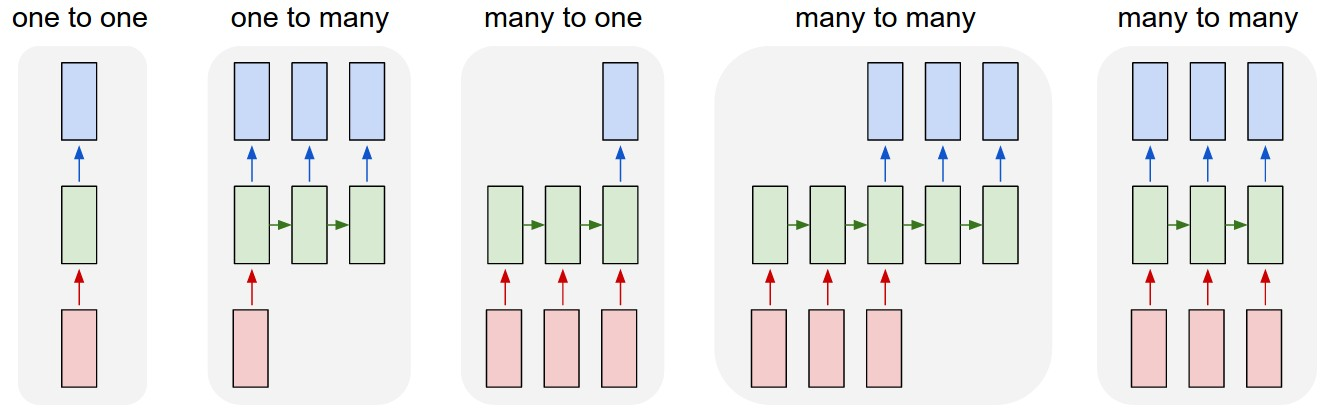
\includegraphics[keepaspectratio]{imagenes/capitulo1/redes_recurrentes/tipos_redes_recurrentes.jpg}}

}

\caption{tipos de redes recurrentes}

\end{figure}%

\begin{itemize}
\tightlist
\item
  One-to-one: Teoricamente posible, pero si solo tenemos una entrada y
  una salida, no nos beneficiaremos de las LSTM. Mejor usar otro tipo de
  red.
\item
  Many-to-one: La entrada está en forma de secuencia y la salida tiene
  un tamaño fijo. En esta categoría entra el análisis de sentimientos.
\item
  One-to-many: En esta opción los datos entran en una forma estándar
  pero la salida es una secuencia. Ejemplos de este formato puede ser la
  catalogación de vídeos donde la entrada es una película y la salida
  una frase.
\item
  Many-to-many: Las salidas y las entradas son secuencias que pueden
  estar sincronizadas (clasificación de vídeos) o retrasadas (traducción
  de un idioma a otro).
\end{itemize}

\subsection{Neurona recurrente o unidad
recurrente}\label{neurona-recurrente-o-unidad-recurrente}

Veamos como funciona una neurona recurrente, la cual recibe una entrada,
produciendo una salida, y enviando esa salida a sí misma, como se
muestra en la siguiente figura:

\begin{figure}[H]

{\centering \pandocbounded{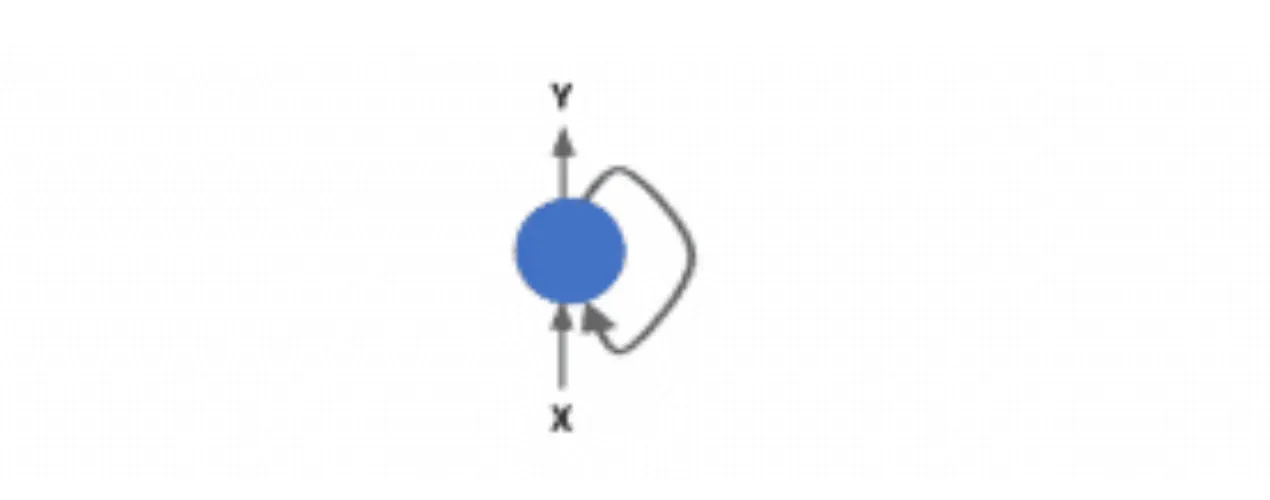
\includegraphics[keepaspectratio]{imagenes/capitulo1/redes_recurrentes/neurona_recurrente.png}}

}

\caption{Neurona recurrente}

\end{figure}%

Una neurona recurrente procesará la información un número de veces
prefijado de veces o timesteps. En cada timestep, esta neurona
recurrente recibe la entrada de la capa anterior, así como su propia
salida del instante de tiempo anterior para generar su salida \(y\).
Podemos representar visualmente esta pequeña red desplegada en el eje
del tiempo como se muestra en la figura:

\begin{figure}[H]

{\centering \pandocbounded{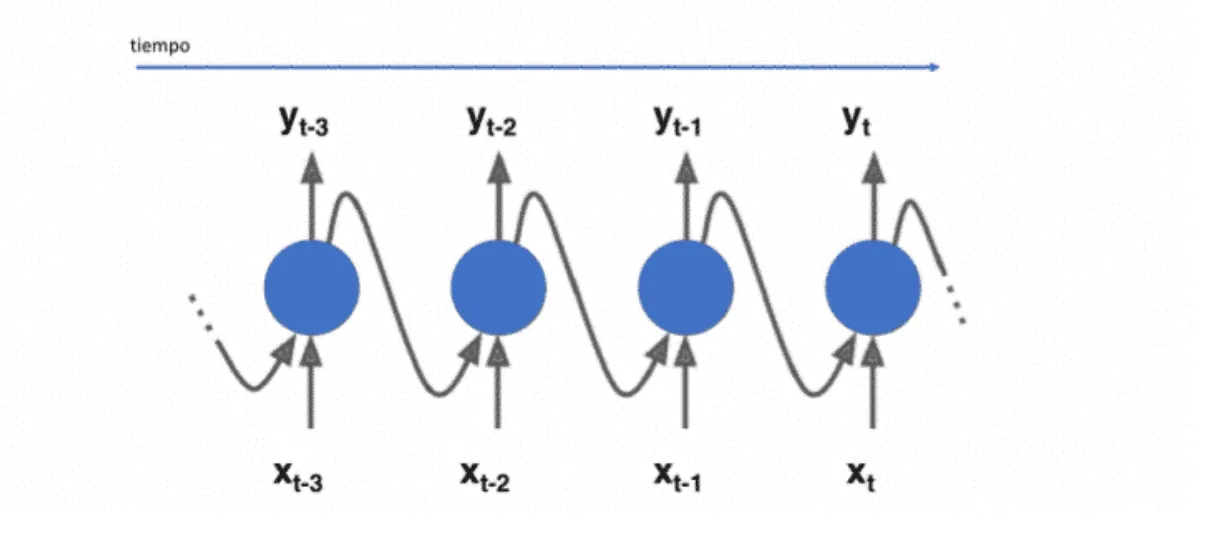
\includegraphics[keepaspectratio]{imagenes/capitulo1/redes_recurrentes/neurona_recurrente_largo_tiempo.png}}

}

\caption{Neurona recurrente a lo largo del tiempo}

\end{figure}%

La secuencia la representamos por \(X_{t-3} , X_{t-2} , X_{t-1} , X_t\)
. En este caso el sub índice indica el orden de las instancias. El flujo
de la información en pasos temporales adyacentes en la capa oculta va a
permitir a la red disponer de un recuerdo de lo ocurrido en su pasado.

Siguiendo esta misma idea, una capa de neuronas recurrentes se puede
implementar de tal manera que, en cada instante de tiempo, cada neurona
recurrente recibe dos entradas, la entrada correspondiente de la capa
anterior y a su vez la salida del instante anterior de la misma capa.

Fijemonos más en detalle en la neurona recurrente para ver el proceso
iterativo:

\begin{figure}[H]

{\centering \pandocbounded{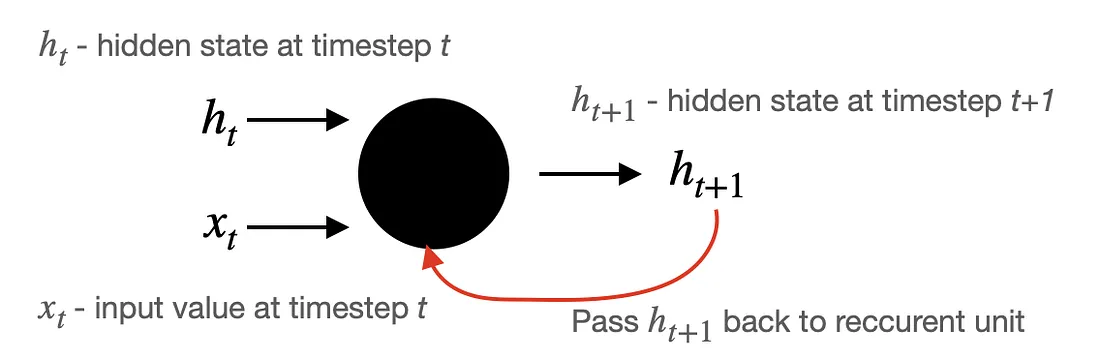
\includegraphics[keepaspectratio]{imagenes/capitulo1/redes_recurrentes/red_recurrente_paso1.png}}

}

\caption{RED recurrente. Paso 1}

\end{figure}%

En el timestep inicial, la neurona recurrente recibe el estado oculto
\(h_t\) inicializado a 0. El output de la neurona, el estado oculto
\(h_{t+1}\) es pasado de vuelta a la neurona junto con la entrada del
siguiente timestep \(x_{t+1}\)

\begin{figure}[H]

{\centering \pandocbounded{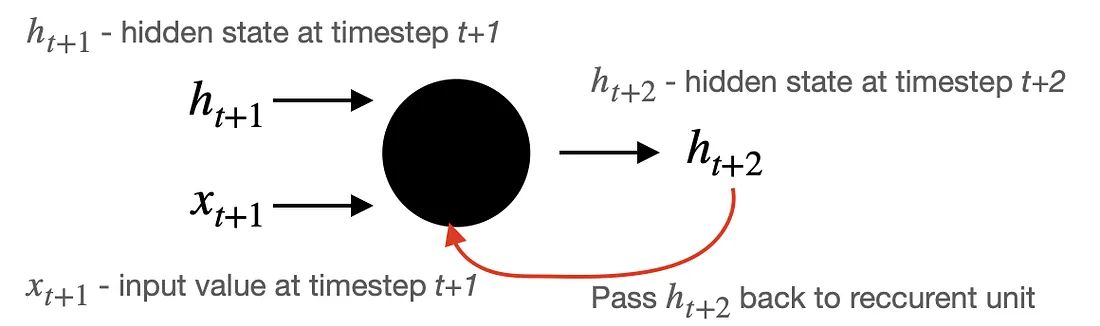
\includegraphics[keepaspectratio]{imagenes/capitulo1/redes_recurrentes/red_recurrente_paso2.png}}

}

\caption{RED recurrente. Paso 2}

\end{figure}%

En esta nueva iteración, vemos como la información previa hasta el
timestep \(t+2\) se almacena en el hidden state \(h_{t+2}\). Este
\(h_{t+2}\) se pasará de vuelta a la neurona recurrente junto con la
entrada \(x_{t+2}\) para hacer una nueva iteración, y así sucesivamente.

\textbf{Nota:} Dado que \(h_0\) se inicializa a cero, se puede obviar
ese valor y cambiar la notación anterior para usar \(h_{t-1}\) donde
antes usábamos \(h_t\) para hacer más hincapié en que se trata de
información proveniente del pasado.

Veamos matemáticamente cómo la información se conserva a lo largo del
tiempo:

\begin{figure}[H]

{\centering \pandocbounded{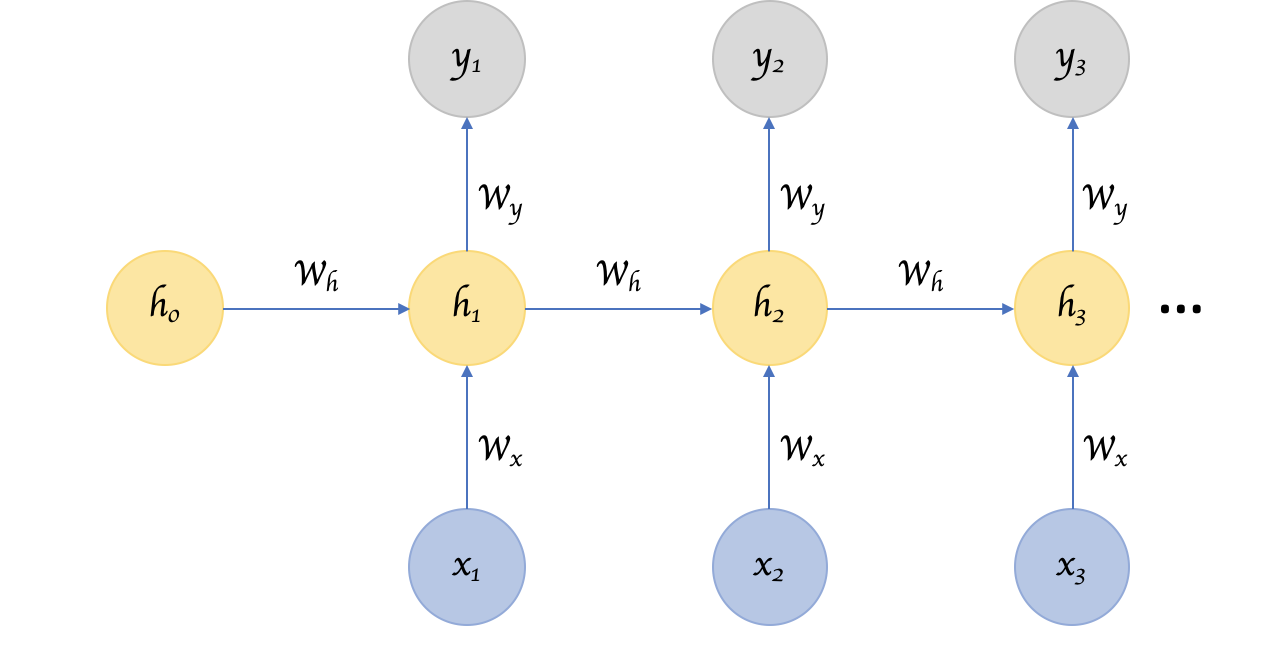
\includegraphics[keepaspectratio]{imagenes/capitulo1/redes_recurrentes/red_recurrente.png}}

}

\caption{Red recurrente}

\end{figure}%

Dada la red recurrente de la imagen, La entrada de la capa oculta (la
llamaremos \(z_t\)), se tiene que calcular a través de la suma de las
multiplicaciones de las matrices ponderadas con los respectivos vectores
y añadir el sesgo:

\[ z_t = W_x \cdot x_t + W_h \cdot h_{t-1} + b\]

El estado oculto con su función de activación se calcula con:

\[h_t = g(z_t) = g(W_x \cdot x_t + W_h \cdot h_{t-1} + b_h)\]

Finalmente, la activación de las unidades de salida se calcula de la
siguiente forma:

\[y_t = f(W_y \cdot h_t + b_y)\]

Observando esto, vemos el concepto de recurrencia y la memoria en las
redes recurrentes: La salida \(y_t\) depende del estado oculto \(h_t\),
pero a su vez, \(h_t\) no solo depende de la entrada actual \(x_t\),
sino también de \(h_{t-1}\). Es así como la información se conserva a lo
largo del tiempo.

Dado que la salida de una neurona recurrente en un instante de tiempo
determinado es una función de entradas de los instantes de tiempo
anteriores, se podría decir que una neurona recurrente tiene en cierta
forma memoria. La parte de una red neuronal que preserva un estado a
través del tiempo se suele llamar celda de memoria.

Y precisamente esta ``memoria interna'' es lo que hace de este tipo de
redes muy adecuadas para problemas de aprendizaje automático que
involucran datos secuenciales. Gracias a su memoria interna, las RNN
pueden recordar información relevante sobre la entrada que recibieron,
lo que les permite ser más precisas en la predicción de lo que vendrá
después manteniendo información de contexto a diferencia de los otros
tipos de redes que hemos visto, que no pueden recordar acerca de lo que
ha sucedido en el pasado, excepto lo reflejado en su entrenamiento a
través de sus pesos.

Proporcionar modelos con memoria y permitirles modelar la evolución
temporal de las señales es un factor clave en muchas tareas de
clasificación y traducción de secuencias en las que los RNN sobresalen,
como la traducción automática, el modelado del lenguaje o el
reconocimiento de voz, entre muchas otras áreas.

Para ilustrar el concepto de ``memoria'' de una RNN, imaginemos que
tenemos una red neuronal como las vistas en capítulos anteriores, le
pasamos la palabra ``neurona'' como entrada y esta red procesa la
palabra carácter a carácter. En el momento en que alcanza el carácter
``r'', ya se ha olvidado de ``n'', ``e'' y ``u'', lo que hace que sea
casi imposible para la red neuronal predecir qué letra vendrá después.
Pero, en cambio, una RNN permite recordar precisamente esto.
Conceptualmente, la RNN tiene como entradas el presente y el pasado
reciente. Esto es importante porque la secuencia de datos contiene
información crucial para saber lo que viene a continuación.

\subsection{Redes recurrentes clásicas: Elman y
Jordan}\label{redes-recurrentes-cluxe1sicas-elman-y-jordan}

Existen diferentes planteamientos de redes recurrentes. Las primeras
redes recurrentes consideradas clásicas y que todavía gozan de cierta
popularidad por sus aplicaciones son las redes de Elman y de Jordan.

En las redes de Elman, las entradas de estas neuronas se toman desde las
salidas de las neuronas de una de las capas ocultas, y sus salidas se
conectan de nuevo en las entradas de esta misma capa, lo que proporciona
una especie de memoria sobre el estado anterior de dicha capa. El
esquema es como en la Figura 78, donde X es la entrada, S la salida y el
nodo amarillo es la neurona de la capa de contexto.

\begin{figure}[H]

{\centering \pandocbounded{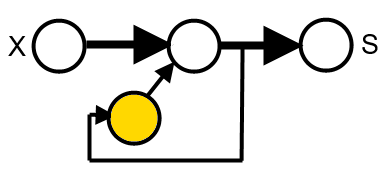
\includegraphics[keepaspectratio]{imagenes/capitulo1/redes_recurrentes/red_neuronal_elman.png}}

}

\caption{Red neuronal de Elman}

\end{figure}%

En las redes de Jordan, la diferencia está en que la entrada de las
neuronas de la capa de contexto se toma desde la salida de la red:

\begin{figure}[H]

{\centering \pandocbounded{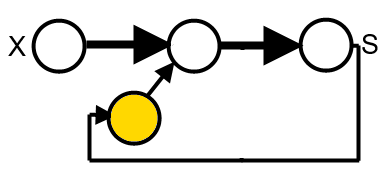
\includegraphics[keepaspectratio]{imagenes/capitulo1/redes_recurrentes/red_neuronal_jordan.png}}

}

\caption{Red neuronal de Jordan}

\end{figure}%

Precisamente por esta característica de memoria son apropiadas para
modelar series temporales.

¿Por qué necesitariamos una nueva arquitectura, si ya hemos visto que
las redes recurrentes tienen memoria?

Las redes neuronales recurrentes (RNN) son especialmente adecuadas para
trabajar con datos secuenciales y temporales, como series de tiempo,
texto y señales. Sin embargo, presentan un problema conocido como el
problema de la desaparición del gradiente (gradient vanishing). Veamos
por qué ocurre este problema:

\begin{itemize}
\item
  Backpropagation Through Time (BPTT): Las RNNs se entrenan utilizando
  una extensión de la retropropagación llamada ``Backpropagation Through
  Time'' (BPTT). Este proceso implica descomponer el gradiente del error
  con respecto a cada peso a través de todas las secuencias temporales.
\item
  Gradientes Muy Pequeños: Durante BPTT, los gradientes pueden volverse
  extremadamente pequeños debido a la multiplicación repetida de
  derivadas (que suelen ser números entre 0 y 1) a lo largo de muchas
  capas de tiempo. Este fenómeno se llama ``vanishing gradients''
  (desaparición del gradiente).
\item
  Efecto en el Entrenamiento: Cuando los gradientes se vuelven muy
  pequeños, las actualizaciones de los pesos son insignificantes, lo que
  hace que la red no pueda aprender de manera efectiva. Esto es
  especialmente problemático para las dependencias a largo plazo, donde
  las conexiones relevantes se pierden en las iteraciones temporales.
\end{itemize}

De ahí surgieron las redes LSTM, diseñadas para abordar el problema de
la desaparición del gradiente.

\subsection{Red Long-Short Term Memory
(LSTM)}\label{red-long-short-term-memory-lstm}

Las redes Long-Short Term Memory(LSTM) son una extensión de las redes
neuronales recurrentes que básicamente amplían su memoria para aprender
de experiencias importantes que han pasado hace mucho tiempo. Las LSTM
permiten a las RNN recordar sus entradas durante un largo período de
tiempo. Esto se debe a que LSTM contiene su información en la memoria,
que puede considerarse similar a la memoria de un ordenador, en el
sentido de que una neurona de una LSTM puede leer, escribir y borrar
información de su memoria.

Esta memoria se puede ver como una ``celda de estado'', donde la celda
decide si almacenar o eliminar información dentro (abriendo la puerta o
no para almacenar), en función de la importancia que asigna a la
información que está recibiendo. La asignación de importancia se decide
a través de los pesos. Esto lo podemos ver como que aprende con el
tiempo qué información es importante y cuál no.

En una neurona LSTM hay tres puertas a estas ``celdas'' que controlan el
flujo de información: puerta de entrada (input gate), puerta de olvidar
(forget gate) y puerta de salida (output gate). Estas puertas determinan
si se permite o no una nueva entrada, se elimina la información porque
no es importante o se deja que afecte a la salida en el paso de tiempo
actual.

La puerta de entrada controla cuándo la información nueva puede entrar
en la memoria. La puerta del olvido controla cuándo se olvida una parte
de la información, lo que permite a la celda recordar datos nuevos. Por
último, la puerta de salida controla cuándo se utiliza en el resultado
de la celda la información que está contenida en la celda. Las celdas
pueden contener ponderaciones, que nos sirven para controlar a cada
puerta.

Las puertas en una LSTM son análogas a una forma sigmoide, lo que
significa que van de 0 a 1 en la forma que hemos visto en capítulos
anteriores. El hecho de que sean análogas a una función de activación
sigmoide permite incorporarlas (matemáticamente hablando) al proceso de
Backpropagation.

Veamos una representación gráfica:

\begin{figure}[H]

{\centering \pandocbounded{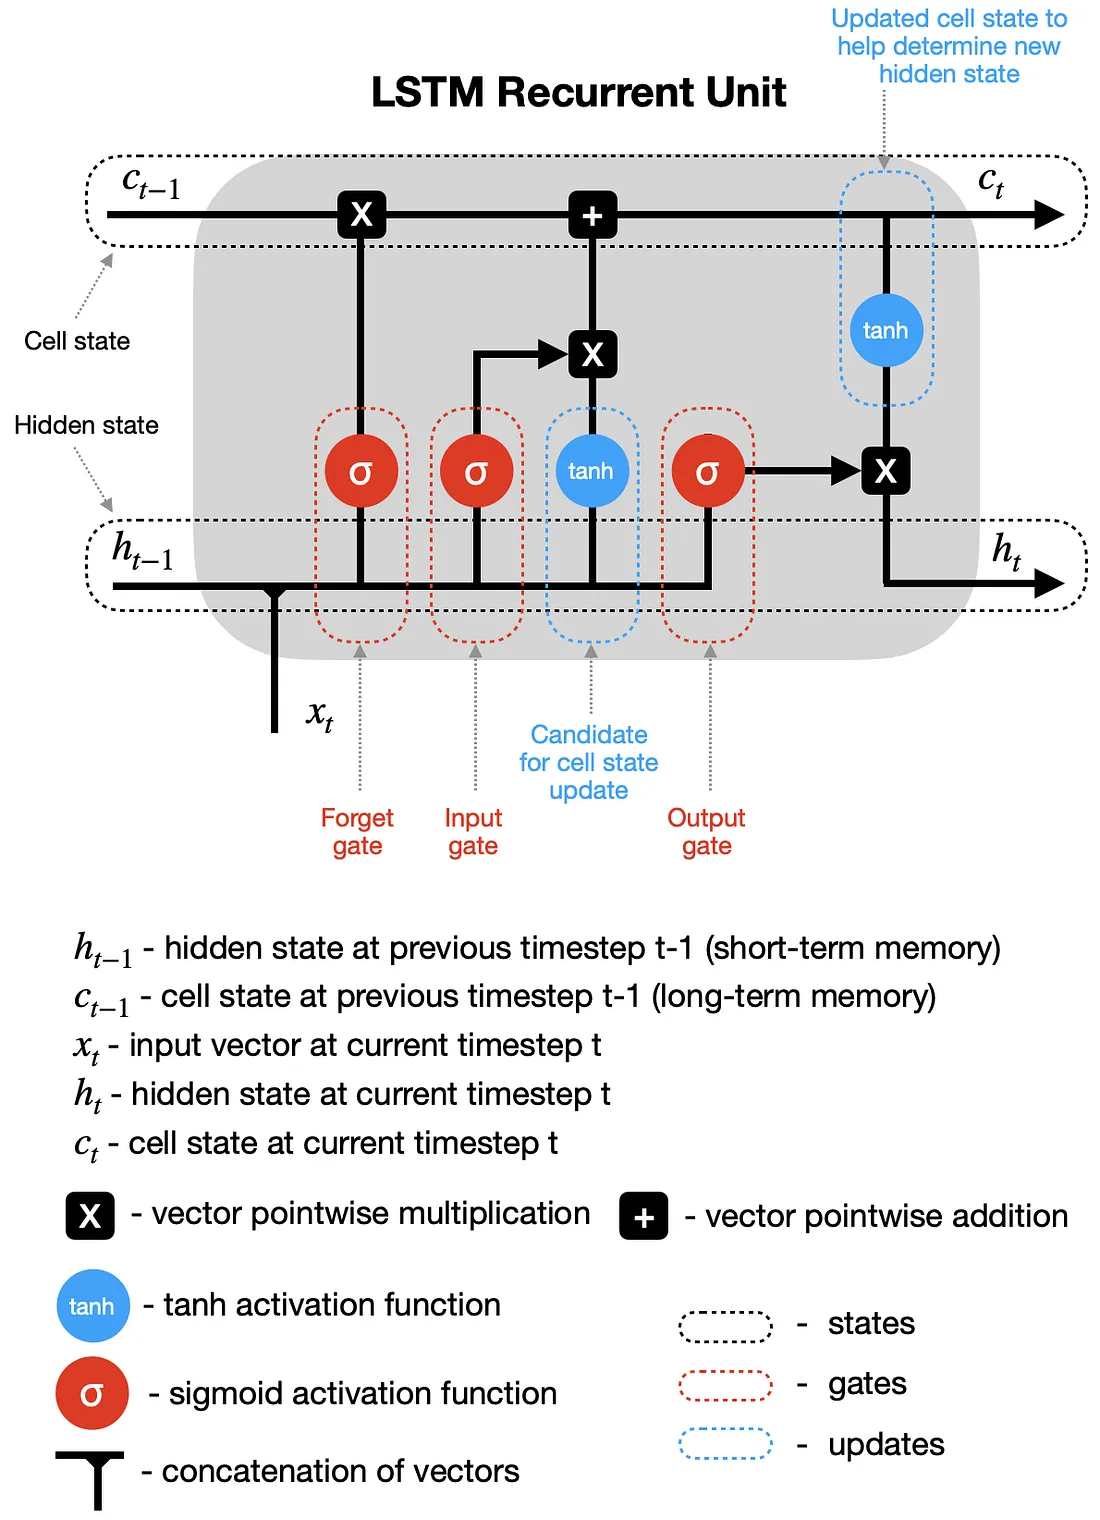
\includegraphics[keepaspectratio]{imagenes/capitulo1/redes_recurrentes/red_neuronal_ltsm.png}}

}

\caption{LSTM}

\end{figure}%

Los pasos serían los siguientes:

\begin{enumerate}
\def\labelenumi{\arabic{enumi}.}
\item
  Estado oculto y nuevos datos: El estado oculto del anterior timestep
  \(h_{t-1}\) y el input del actual timestep \(x_t\) son combinados
  antes de pasar por varias puertas.
\item
  Puerta del olvido: Esta puerta controla qué información debe ser
  olvidada. Dado que la función sigmoide varía entre 0 y 1, establece
  qué valores en el estado de la celda deben ser descartados
  (multiplicados por 0), recordados (multiplicados por 1) o parcialmente
  recordados (multiplicados por algún valor entre 0 y 1).
\item
  Puerta de entrada: Ayuda a identificar elementos importantes que
  necesitan ser añadidos a la celda de estado. Nota que los resultados
  de la puerta de entrada se multiplican por el candidato del estado de
  la celda, añadiendo al estado de la celda solo la información
  considerada importante por la puerta de entrada.
\item
  Actualizar el estado de la celda: primero, el estado de la celda
  anterior (\(c_{t-1}\)) se multiplica por los resultados de la puerta
  de olvido. Luego, añadimos nueva información de {[}puerta de entrada ×
  candidato del estado de la celda{]} para obtener el último estado de
  la celda (\(c_t\)).
\item
  Actualizar el estado oculto: la última parte es actualizar el estado
  oculto. El último estado de la celda (\(c_t\)) se pasa a través de la
  función de activación tanh y se multiplica por los resultados de la
  puerta de salida.
\end{enumerate}

Finalmente, el último estado de la celda (\(c_t\)) y el estado oculto
(\(h_t\)) regresan a la unidad recurrente, y el proceso se repite en el
tiempo \(t+1\). El bucle continúa hasta que llegamos al final de la
secuencia.

\subsection{Red GRU}\label{red-gru}

La red GRU (Gated Recurrent Unit) constituye un enfoque más reciente que
las LSTM y fue propuesto en el año 2014 por Cho et al.~Estas redes
tienen una arquitectura más sencilla, lo que implica que es más
eficiente computacionalmente y el rendimiento es comparable con las
LSTM.

Esta arquitectura incluye dos puertas: una puerta de actualización y una
puerta de reset. La puerta de actualización indica cuánto del contenido
de las celdas anteriores hay que mantener. La puerta de reset define
cómo incorporar la nueva entrada con los contenidos anteriores de la
celda. Una red GRU puede ser una RNN estándar simplemente estableciendo
la puerta de reset a 1 y la puerta de actualización a 0.

Para ampliar información sobre las redes GRU se puede consultar el
documento escrito por Junyoung Chung et al.~(2014) titulado ``Evaluación
empírica de redes neuronales recurrentes cerradas en modelo secuencial
``

GRU es similar a LSTM, pero tiene menos puertas de control. Además, se
basa únicamente en un estado oculto para la transferencia de memoria
entre unidades recurrentes, por lo que no hay un estado de celda
separado. Analicemos este diagrama simplificado de GRU en detalle (pesos
y sesgos no mostrados).

\begin{figure}[H]

{\centering \pandocbounded{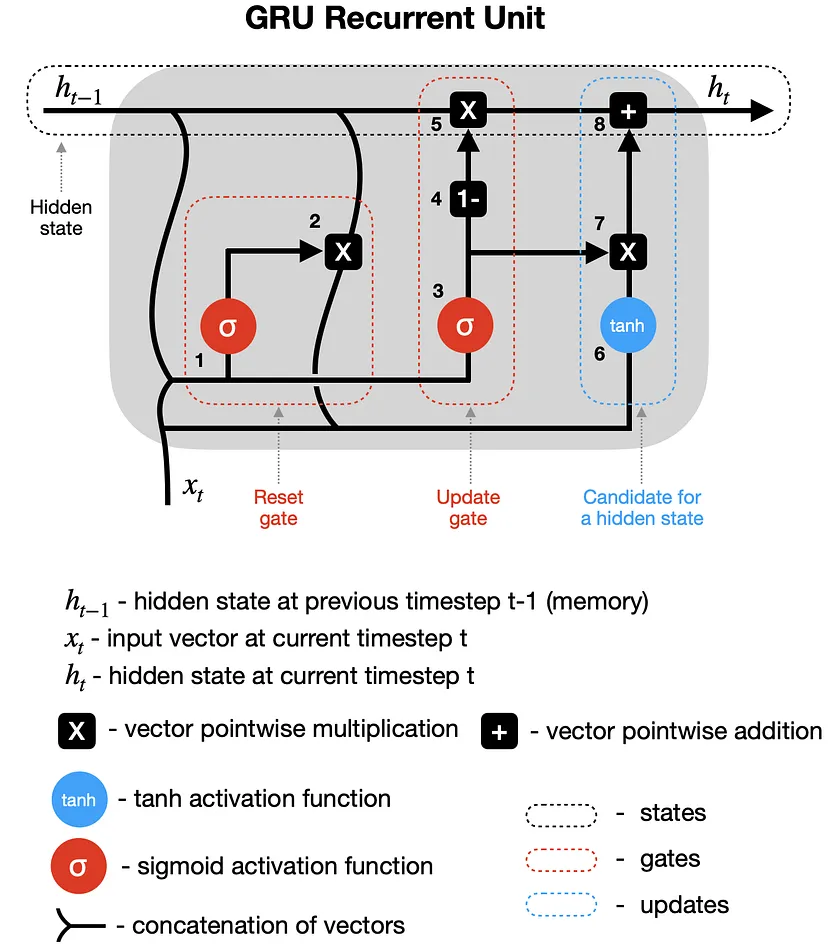
\includegraphics[keepaspectratio]{imagenes/capitulo1/redes_recurrentes/red_neuronal_gru.png}}

}

\caption{Red GRU}

\end{figure}%

1--2 Puerta de reset: el estado oculto anterior (\(h_{t-1}\)) y la
entrada actual (\(x_t\)) se combinan (multiplicados por sus respectivos
pesos y con el sesgo añadido) y se pasan a través de una puerta de
reset. Dado que la función sigmoide varía entre 0 y 1, el primer paso
establece qué valores deben ser descartados (0), recordados (1) o
parcialmente retenidos (entre 0 y 1). El segundo paso reinicia el estado
oculto anterior multiplicándolo con las salidas del primer paso.

3--4--5 Puerta de actualización: el tercer paso puede parecer análogo al
primer paso, pero ten en cuenta que los pesos y sesgos utilizados para
escalar estos vectores son diferentes, proporcionando una salida
sigmoide distinta. Entonces, después de pasar un vector combinado a
través de una función sigmoide, lo restamos de un vector que contiene
todos 1s (paso cuatro) y lo multiplicamos por el estado oculto anterior
(paso cinco). Esa es una parte de la actualización del estado oculto con
nueva información.

6--7--8 Candidato para el estado oculto: después de reiniciar un estado
oculto anterior en el paso dos, las salidas se combinan con nuevas
entradas (\(x_t\)), multiplicándolas por sus respectivos pesos y
añadiendo sesgos antes de pasar a través de una función de activación
tanh (paso seis). Luego, el candidato para el estado oculto se
multiplica por los resultados de una puerta de actualización (paso
siete) y se añade al \(h_{t-1}\) previamente modificado para formar el
nuevo estado oculto \(h_t\).

A continuación veremos como trabajar con estos modelos en la práctica.
Las librerías que utilizaremos serán las siguientes:

\begin{Shaded}
\begin{Highlighting}[numbers=left,,]

\CommentTok{\# Tensorflow / Keras}
\ImportTok{from}\NormalTok{ tensorflow }\ImportTok{import}\NormalTok{ keras }\CommentTok{\# for building Neural Networks}
\ImportTok{from}\NormalTok{ keras.models }\ImportTok{import}\NormalTok{ Sequential }\CommentTok{\# for creating a linear stack of layers for our Neural Network}
\ImportTok{from}\NormalTok{ keras }\ImportTok{import}\NormalTok{ Input }\CommentTok{\# for instantiating a keras tensor}
\ImportTok{from}\NormalTok{ keras.layers }\ImportTok{import}\NormalTok{ Embedding, LSTM, Dense, Dropout, SimpleRNN }\CommentTok{\# for creating regular densely{-}connected NN layers and RNN layers}
\ImportTok{from}\NormalTok{ tensorflow.keras.datasets }\ImportTok{import}\NormalTok{ imdb}
\ImportTok{from}\NormalTok{ keras.preprocessing }\ImportTok{import}\NormalTok{ sequence}
\ImportTok{from}\NormalTok{ keras.layers }\ImportTok{import}\NormalTok{ Bidirectional, RepeatVector, TimeDistributed }\CommentTok{\# for creating layers inside the Neural Network}
\ImportTok{from}\NormalTok{ tensorflow.keras.utils }\ImportTok{import}\NormalTok{ pad\_sequences}

\CommentTok{\# Data manipulation}
\ImportTok{import}\NormalTok{ pandas }\ImportTok{as}\NormalTok{ pd }\CommentTok{\# for data manipulation}
\ImportTok{import}\NormalTok{ numpy }\ImportTok{as}\NormalTok{ np }\CommentTok{\# for data manipulation}
\ImportTok{import}\NormalTok{ math }\CommentTok{\# to help with data reshaping of the data}

\CommentTok{\# Sklearn}
\ImportTok{import}\NormalTok{ sklearn }\CommentTok{\# for model evaluation}
\ImportTok{from}\NormalTok{ sklearn.model\_selection }\ImportTok{import}\NormalTok{ train\_test\_split }\CommentTok{\# for splitting the data into train and test samples}
\ImportTok{from}\NormalTok{ sklearn.metrics }\ImportTok{import}\NormalTok{ mean\_squared\_error }\CommentTok{\# for model evaluation metrics}
\ImportTok{from}\NormalTok{ sklearn.preprocessing }\ImportTok{import}\NormalTok{ MinMaxScaler }\CommentTok{\# for feature scaling}

\CommentTok{\# Visualization}
\ImportTok{import}\NormalTok{ bctools }\ImportTok{as}\NormalTok{ bc}
\ImportTok{import}\NormalTok{ plotly}
\ImportTok{import}\NormalTok{ plotly.express }\ImportTok{as}\NormalTok{ px}
\ImportTok{import}\NormalTok{ plotly.graph\_objects }\ImportTok{as}\NormalTok{ go}
\end{Highlighting}
\end{Shaded}

\subsection{Ejemplo: Predicción de series
temporales}\label{ejemplo-predicciuxf3n-de-series-temporales}

Trabajaremos con los
\href{https://www.kaggle.com/datasets/jsphyg/weather-dataset-rattle-package}{datos
abiertos del clima en Australia}. En este caso, tenemos la temperatura
minima y maxima diaria de varias ciudades. Nos crearermos la variable
\texttt{MedTemp} como la mediana entrelas temperaturas máxima y minima e
intentaremos predecir el valor de esta variable para el día siguiente.
En nuestro caso, solo nos interesará hacer las predicciones para una
única ciudad, Canberra, por lo que obviaremos el resto.

\begin{Shaded}
\begin{Highlighting}[numbers=left,,]
\CommentTok{\# Set Pandas options to display more columns}
\NormalTok{pd.options.display.max\_columns}\OperatorTok{=}\DecValTok{10}

\CommentTok{\# Read in the weather data csv}
\NormalTok{df}\OperatorTok{=}\NormalTok{pd.read\_csv(}\StringTok{\textquotesingle{}weatherAUS.csv\textquotesingle{}}\NormalTok{, encoding}\OperatorTok{=}\StringTok{\textquotesingle{}utf{-}8\textquotesingle{}}\NormalTok{)}

\CommentTok{\# Convert dates to year{-}months}
\NormalTok{df[}\StringTok{\textquotesingle{}Year{-}Month\textquotesingle{}}\NormalTok{]}\OperatorTok{=}\NormalTok{ (pd.to\_datetime(df[}\StringTok{\textquotesingle{}Date\textquotesingle{}}\NormalTok{], yearfirst}\OperatorTok{=}\VariableTok{True}\NormalTok{)).dt.strftime(}\StringTok{\textquotesingle{}\%Y{-}\%m\textquotesingle{}}\NormalTok{)}

\CommentTok{\# Drop records where target MinTemp=NaN or MaxTemp=NaN}
\NormalTok{df}\OperatorTok{=}\NormalTok{df[pd.isnull(df[}\StringTok{\textquotesingle{}MinTemp\textquotesingle{}}\NormalTok{])}\OperatorTok{==}\VariableTok{False}\NormalTok{]}
\NormalTok{df}\OperatorTok{=}\NormalTok{df[pd.isnull(df[}\StringTok{\textquotesingle{}MaxTemp\textquotesingle{}}\NormalTok{])}\OperatorTok{==}\VariableTok{False}\NormalTok{]}

\CommentTok{\# Median daily temperature (mid point between Daily Max and Daily Min)}
\NormalTok{df[}\StringTok{\textquotesingle{}MedTemp\textquotesingle{}}\NormalTok{]}\OperatorTok{=}\NormalTok{df[[}\StringTok{\textquotesingle{}MinTemp\textquotesingle{}}\NormalTok{, }\StringTok{\textquotesingle{}MaxTemp\textquotesingle{}}\NormalTok{]].median(axis}\OperatorTok{=}\DecValTok{1}\NormalTok{)}

\NormalTok{dfCan}\OperatorTok{=}\NormalTok{df[df[}\StringTok{\textquotesingle{}Location\textquotesingle{}}\NormalTok{]}\OperatorTok{==}\StringTok{\textquotesingle{}Canberra\textquotesingle{}}\NormalTok{].copy()}

\CommentTok{\# Show a snaphsot of data}
\NormalTok{dfCan}
\end{Highlighting}
\end{Shaded}

Graficamos los datos para ver como es la serie temporal:

\begin{Shaded}
\begin{Highlighting}[numbers=left,,]
\CommentTok{\# Plot daily median temperatures in Canberra}
\NormalTok{fig }\OperatorTok{=}\NormalTok{ go.Figure()}


\NormalTok{fig.add\_trace(go.Scatter(x}\OperatorTok{=}\NormalTok{dfCan[}\StringTok{\textquotesingle{}Date\textquotesingle{}}\NormalTok{],}
\NormalTok{                         y}\OperatorTok{=}\NormalTok{dfCan[}\StringTok{\textquotesingle{}MedTemp\textquotesingle{}}\NormalTok{],}
\NormalTok{                         mode}\OperatorTok{=}\StringTok{\textquotesingle{}lines\textquotesingle{}}\NormalTok{,}
\NormalTok{                         name}\OperatorTok{=}\StringTok{\textquotesingle{}Median Temperature\textquotesingle{}}\NormalTok{,}
\NormalTok{                         opacity}\OperatorTok{=}\FloatTok{0.8}\NormalTok{,}
\NormalTok{                         line}\OperatorTok{=}\BuiltInTok{dict}\NormalTok{( width}\OperatorTok{=}\DecValTok{1}\NormalTok{)}
\NormalTok{                        ))}

\CommentTok{\# Update axes lines}
\NormalTok{fig.update\_xaxes(showgrid}\OperatorTok{=}\VariableTok{True}\NormalTok{, gridwidth}\OperatorTok{=}\DecValTok{1}\NormalTok{, gridcolor}\OperatorTok{=}\StringTok{\textquotesingle{}lightgrey\textquotesingle{}}\NormalTok{,}
\NormalTok{                 zeroline}\OperatorTok{=}\VariableTok{True}\NormalTok{, zerolinewidth}\OperatorTok{=}\DecValTok{1}\NormalTok{, zerolinecolor}\OperatorTok{=}\StringTok{\textquotesingle{}lightgrey\textquotesingle{}}\NormalTok{,}
\NormalTok{                 showline}\OperatorTok{=}\VariableTok{True}\NormalTok{, linewidth}\OperatorTok{=}\DecValTok{1}\NormalTok{, linecolor}\OperatorTok{=}\StringTok{\textquotesingle{}black\textquotesingle{}}\NormalTok{,}
\NormalTok{                 title}\OperatorTok{=}\StringTok{\textquotesingle{}Date\textquotesingle{}}
\NormalTok{                )}

\NormalTok{fig.update\_yaxes(showgrid}\OperatorTok{=}\VariableTok{True}\NormalTok{, gridwidth}\OperatorTok{=}\DecValTok{1}\NormalTok{, gridcolor}\OperatorTok{=}\StringTok{\textquotesingle{}lightgrey\textquotesingle{}}\NormalTok{,}
\NormalTok{                 zeroline}\OperatorTok{=}\VariableTok{True}\NormalTok{, zerolinewidth}\OperatorTok{=}\DecValTok{1}\NormalTok{, zerolinecolor}\OperatorTok{=}\StringTok{\textquotesingle{}lightgrey\textquotesingle{}}\NormalTok{,}
\NormalTok{                 showline}\OperatorTok{=}\VariableTok{True}\NormalTok{, linewidth}\OperatorTok{=}\DecValTok{1}\NormalTok{, linecolor}\OperatorTok{=}\StringTok{\textquotesingle{}black\textquotesingle{}}\NormalTok{,}
\NormalTok{                 title}\OperatorTok{=}\StringTok{\textquotesingle{}Degrees Celsius\textquotesingle{}}
\NormalTok{                )}

\CommentTok{\# Set figure title}
\NormalTok{fig.update\_layout(}
\NormalTok{    title}\OperatorTok{=}\BuiltInTok{dict}\NormalTok{(text}\OperatorTok{=}\StringTok{"Temperatures in Canberra"}\NormalTok{,}
\NormalTok{    font}\OperatorTok{=}\BuiltInTok{dict}\NormalTok{(color}\OperatorTok{=}\StringTok{\textquotesingle{}black\textquotesingle{}}\NormalTok{))}
\NormalTok{)}

\NormalTok{fig.show()}
\end{Highlighting}
\end{Shaded}

\begin{figure}[H]

{\centering \pandocbounded{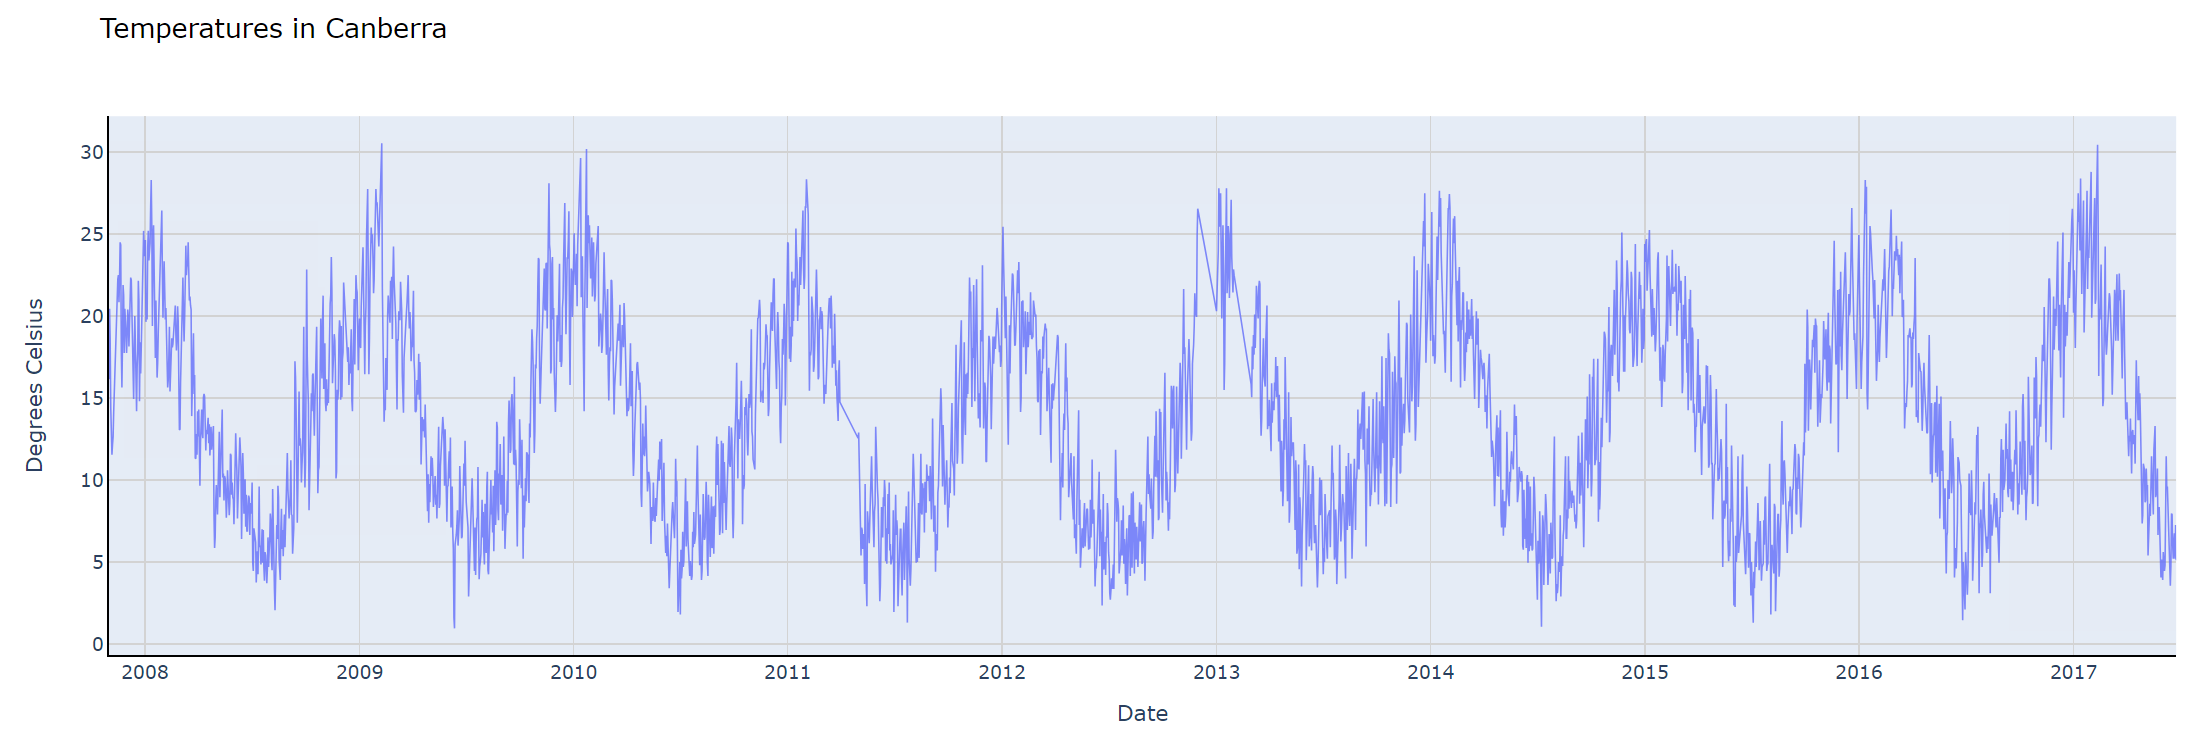
\includegraphics[keepaspectratio]{imagenes/capitulo1/redes_recurrentes/serie_temporal.png}}

}

\caption{Serie temporal}

\end{figure}%

\begin{Shaded}
\begin{Highlighting}[numbers=left,,]
\KeywordTok{def}\NormalTok{ prep\_data(datain, time\_step):}
    \CommentTok{\# 1. y{-}array}
    \CommentTok{\# First, create an array with indices for y elements based on the chosen time\_step}
\NormalTok{    y\_indices }\OperatorTok{=}\NormalTok{ np.arange(start}\OperatorTok{=}\NormalTok{time\_step, stop}\OperatorTok{=}\BuiltInTok{len}\NormalTok{(datain), step}\OperatorTok{=}\NormalTok{time\_step)}
    \CommentTok{\# Create y array based on the above indices}
\NormalTok{    y\_tmp }\OperatorTok{=}\NormalTok{ datain[y\_indices]}

    \CommentTok{\# 2. X{-}array}
    \CommentTok{\# We want to have the same number of rows for X as we do for y}
\NormalTok{    rows\_X }\OperatorTok{=} \BuiltInTok{len}\NormalTok{(y\_tmp)}
    \CommentTok{\# Since the last element in y\_tmp may not be the last element of the datain,}
    \CommentTok{\# let\textquotesingle{}s ensure that X array stops with the last y}
\NormalTok{    X\_tmp }\OperatorTok{=}\NormalTok{ datain[}\BuiltInTok{range}\NormalTok{(time\_step}\OperatorTok{*}\NormalTok{rows\_X)]}
    \CommentTok{\# Now take this array and reshape it into the desired shape}
\NormalTok{    X\_tmp }\OperatorTok{=}\NormalTok{ np.reshape(X\_tmp, (rows\_X, time\_step, }\DecValTok{1}\NormalTok{))}
    \ControlFlowTok{return}\NormalTok{ X\_tmp, y\_tmp}
\end{Highlighting}
\end{Shaded}

La función anterior nos ayudara a reestructurar los datos para cualquier
número de timesteps. Por ejemplo, si uso 7 timesteps (uso una secuencia
de 7 días para predecir la temperatura el proximo día), la
transformación será así:

\begin{figure}[H]

{\centering \pandocbounded{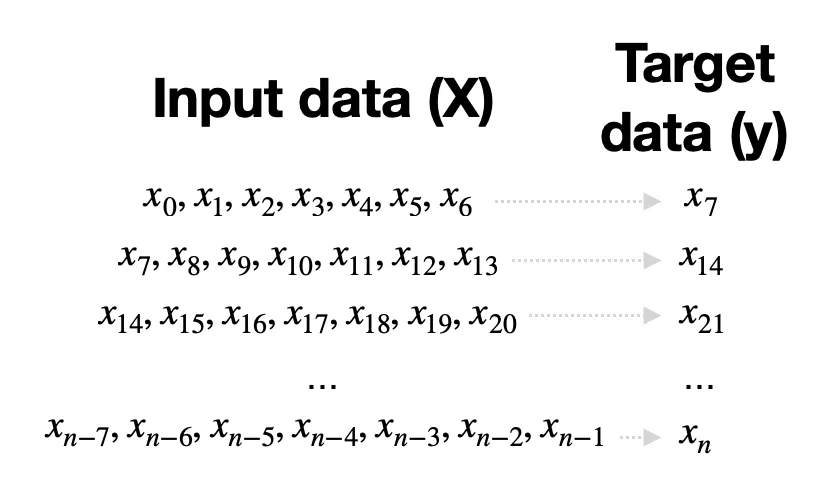
\includegraphics[keepaspectratio]{imagenes/capitulo1/redes_recurrentes/transformacion_datos.png}}

}

\caption{Transformación de datos}

\end{figure}%

Una vez tenemos esto, podemo crear nuestro modelo y entrenarlo:

\begin{Shaded}
\begin{Highlighting}[numbers=left,,]

\CommentTok{\#\#\#\#\# Step 1 {-} Select data for modeling and apply MinMax scaling}
\NormalTok{X}\OperatorTok{=}\NormalTok{dfCan[[}\StringTok{\textquotesingle{}MedTemp\textquotesingle{}}\NormalTok{]]}
\NormalTok{scaler }\OperatorTok{=}\NormalTok{ MinMaxScaler()}
\NormalTok{X\_scaled}\OperatorTok{=}\NormalTok{scaler.fit\_transform(X)}


\CommentTok{\#\#\#\#\# Step 2 {-} Create training and testing samples}
\NormalTok{train\_data, test\_data }\OperatorTok{=}\NormalTok{ train\_test\_split(X\_scaled, test\_size}\OperatorTok{=}\FloatTok{0.2}\NormalTok{, shuffle}\OperatorTok{=}\VariableTok{False}\NormalTok{)}


\CommentTok{\#\#\#\#\# Step 3 {-} Prepare input X and target y arrays using previously defined function}
\NormalTok{time\_step }\OperatorTok{=} \DecValTok{7}
\NormalTok{X\_train, y\_train }\OperatorTok{=}\NormalTok{ prep\_data(train\_data, time\_step)}
\NormalTok{X\_test, y\_test }\OperatorTok{=}\NormalTok{ prep\_data(test\_data, time\_step)}

\CommentTok{\# \#\#\#\#\# Step 4 {-} Specify the structure of a Neural Network}
\NormalTok{model }\OperatorTok{=}\NormalTok{ Sequential(name}\OperatorTok{=}\StringTok{"RNN{-}Model"}\NormalTok{) }\CommentTok{\# Model}
\NormalTok{model.add(Input(shape}\OperatorTok{=}\NormalTok{(time\_step,}\DecValTok{1}\NormalTok{), name}\OperatorTok{=}\StringTok{\textquotesingle{}Input{-}Layer\textquotesingle{}}\NormalTok{)) }\CommentTok{\# Input Layer {-} need to speicfy the shape of inputs}
\NormalTok{model.add(SimpleRNN(units}\OperatorTok{=}\DecValTok{1}\NormalTok{, activation}\OperatorTok{=}\StringTok{\textquotesingle{}tanh\textquotesingle{}}\NormalTok{, name}\OperatorTok{=}\StringTok{\textquotesingle{}Hidden{-}Recurrent{-}Layer\textquotesingle{}}\NormalTok{)) }\CommentTok{\# Hidden Recurrent Layer}
\NormalTok{model.add(Dense(units}\OperatorTok{=}\DecValTok{2}\NormalTok{, activation}\OperatorTok{=}\StringTok{\textquotesingle{}tanh\textquotesingle{}}\NormalTok{, name}\OperatorTok{=}\StringTok{\textquotesingle{}Hidden{-}Layer\textquotesingle{}}\NormalTok{)) }\CommentTok{\# Hidden Layer}
\NormalTok{model.add(Dense(units}\OperatorTok{=}\DecValTok{1}\NormalTok{, activation}\OperatorTok{=}\StringTok{\textquotesingle{}linear\textquotesingle{}}\NormalTok{, name}\OperatorTok{=}\StringTok{\textquotesingle{}Output{-}Layer\textquotesingle{}}\NormalTok{)) }\CommentTok{\# Output Layer, Linear(x) = x}


\CommentTok{\#\#\#\#\# Step 5 {-} Compile keras model}
\NormalTok{model.}\BuiltInTok{compile}\NormalTok{(}
\NormalTok{    optimizer}\OperatorTok{=}\StringTok{\textquotesingle{}adam\textquotesingle{}}\NormalTok{,}
\NormalTok{    loss}\OperatorTok{=}\StringTok{\textquotesingle{}mean\_squared\_error\textquotesingle{}}\NormalTok{, }\CommentTok{\# Loss function to be optimized.}
\NormalTok{    metrics}\OperatorTok{=}\NormalTok{[}\StringTok{\textquotesingle{}MeanSquaredError\textquotesingle{}}\NormalTok{, }\StringTok{\textquotesingle{}MeanAbsoluteError\textquotesingle{}}\NormalTok{], }\CommentTok{\# List of metrics to be evaluated by the model during training and testing.}
\NormalTok{    loss\_weights}\OperatorTok{=}\VariableTok{None}\NormalTok{,}
\NormalTok{    weighted\_metrics}\OperatorTok{=}\VariableTok{None}\NormalTok{,}
\NormalTok{    run\_eagerly}\OperatorTok{=}\VariableTok{None}
\NormalTok{)}


\CommentTok{\# \#\#\#\#\# Step 6 {-} Fit keras model on the dataset}
\NormalTok{model.fit(}
\NormalTok{    X\_train, }\CommentTok{\# input data}
\NormalTok{    y\_train, }\CommentTok{\# target data}
\NormalTok{    batch\_size}\OperatorTok{=}\DecValTok{1}\NormalTok{, }\CommentTok{\# Number of samples per gradient update.}
\NormalTok{    epochs}\OperatorTok{=}\DecValTok{20}\NormalTok{, }\CommentTok{\# default=1, Number of epochs to train the model}
\NormalTok{    validation\_split}\OperatorTok{=}\FloatTok{0.0}\NormalTok{, }\CommentTok{\# default=0.0, Fraction of the training data to be used as validation data. The model will set apart this fraction of the training data, will not train on it, and will evaluate the loss and any model metrics on this data at the end of each epoch.}
\NormalTok{    shuffle}\OperatorTok{=}\VariableTok{True}\NormalTok{, }\CommentTok{\# default=True, Boolean (whether to shuffle the training data before each epoch) or str (for \textquotesingle{}batch\textquotesingle{}).}
\NormalTok{    class\_weight}\OperatorTok{=}\VariableTok{None}\NormalTok{, }\CommentTok{\# default=None, Optional dictionary mapping class indices (integers) to a weight (float) value, used for weighting the loss function (during training only). This can be useful to tell the model to "pay more attention" to samples from an under{-}represented class.}
\NormalTok{    sample\_weight}\OperatorTok{=}\VariableTok{None}\NormalTok{, }\CommentTok{\# default=None, Optional Numpy array of weights for the training samples, used for weighting the loss function (during training only).}
\NormalTok{    initial\_epoch}\OperatorTok{=}\DecValTok{0}\NormalTok{, }\CommentTok{\# Integer, default=0, Epoch at which to start training (useful for resuming a previous training run).}
\NormalTok{    steps\_per\_epoch}\OperatorTok{=}\VariableTok{None}\NormalTok{, }\CommentTok{\# Integer or None, default=None, Total number of steps (batches of samples) before declaring one epoch finished and starting the next epoch. When training with input tensors such as TensorFlow data tensors, the default None is equal to the number of samples in your dataset divided by the batch size, or 1 if that cannot be determined.}
\NormalTok{    validation\_steps}\OperatorTok{=}\VariableTok{None}\NormalTok{, }\CommentTok{\# Only relevant if validation\_data is provided and is a tf.data dataset. Total number of steps (batches of samples) to draw before stopping when performing validation at the end of every epoch.}
\NormalTok{    validation\_batch\_size}\OperatorTok{=}\VariableTok{None}\NormalTok{, }\CommentTok{\# Integer or None, default=None, Number of samples per validation batch. If unspecified, will default to batch\_size.}
\NormalTok{    validation\_freq}\OperatorTok{=}\DecValTok{1} \CommentTok{\# default=1, Only relevant if validation data is provided. If an integer, specifies how many training epochs to run before a new validation run is performed, e.g. validation\_freq=2 runs validation every 2 epochs.}
\NormalTok{    )}


\CommentTok{\#\#\#\#\# Step 7 {-} Make predictions}
\CommentTok{\# Predict the result on training data}
\NormalTok{pred\_train }\OperatorTok{=}\NormalTok{ model.predict(X\_train)}
\CommentTok{\# Predict the result on test data}
\NormalTok{pred\_test }\OperatorTok{=}\NormalTok{ model.predict(X\_test)}

\CommentTok{\#\#\#\#\# Step 8 {-} Model Performance Summary}
\BuiltInTok{print}\NormalTok{(}\StringTok{""}\NormalTok{)}
\BuiltInTok{print}\NormalTok{(}\StringTok{\textquotesingle{}{-}{-}{-}{-}{-}{-}{-}{-}{-}{-}{-}{-}{-}{-}{-}{-}{-}{-}{-}{-} Model Summary {-}{-}{-}{-}{-}{-}{-}{-}{-}{-}{-}{-}{-}{-}{-}{-}{-}{-}{-}{-}\textquotesingle{}}\NormalTok{)}
\NormalTok{model.summary() }\CommentTok{\# print model summary}
\BuiltInTok{print}\NormalTok{(}\StringTok{""}\NormalTok{)}
\BuiltInTok{print}\NormalTok{(}\StringTok{\textquotesingle{}{-}{-}{-}{-}{-}{-}{-}{-}{-}{-}{-}{-}{-}{-}{-}{-}{-}{-}{-}{-} Weights and Biases {-}{-}{-}{-}{-}{-}{-}{-}{-}{-}{-}{-}{-}{-}{-}{-}{-}{-}{-}{-}\textquotesingle{}}\NormalTok{)}
\BuiltInTok{print}\NormalTok{(}\StringTok{"Note, the last parameter in each layer is bias while the rest are weights"}\NormalTok{)}
\BuiltInTok{print}\NormalTok{(}\StringTok{""}\NormalTok{)}
\ControlFlowTok{for}\NormalTok{ layer }\KeywordTok{in}\NormalTok{ model.layers:}
    \BuiltInTok{print}\NormalTok{(layer.name)}
    \ControlFlowTok{for}\NormalTok{ item }\KeywordTok{in}\NormalTok{ layer.get\_weights():}
        \BuiltInTok{print}\NormalTok{(}\StringTok{"  "}\NormalTok{, item)}
\BuiltInTok{print}\NormalTok{(}\StringTok{""}\NormalTok{)}
\BuiltInTok{print}\NormalTok{(}\StringTok{\textquotesingle{}{-}{-}{-}{-}{-}{-}{-}{-}{-}{-} Evaluation on Training Data {-}{-}{-}{-}{-}{-}{-}{-}{-}{-}\textquotesingle{}}\NormalTok{)}
\BuiltInTok{print}\NormalTok{(}\StringTok{"MSE: "}\NormalTok{, mean\_squared\_error(y\_train, pred\_train))}
\BuiltInTok{print}\NormalTok{(}\StringTok{""}\NormalTok{)}

\BuiltInTok{print}\NormalTok{(}\StringTok{\textquotesingle{}{-}{-}{-}{-}{-}{-}{-}{-}{-}{-} Evaluation on Test Data {-}{-}{-}{-}{-}{-}{-}{-}{-}{-}\textquotesingle{}}\NormalTok{)}
\BuiltInTok{print}\NormalTok{(}\StringTok{"MSE: "}\NormalTok{, mean\_squared\_error(y\_test, pred\_test))}
\BuiltInTok{print}\NormalTok{(}\StringTok{""}\NormalTok{)}
\end{Highlighting}
\end{Shaded}

\begin{figure}[H]

{\centering \pandocbounded{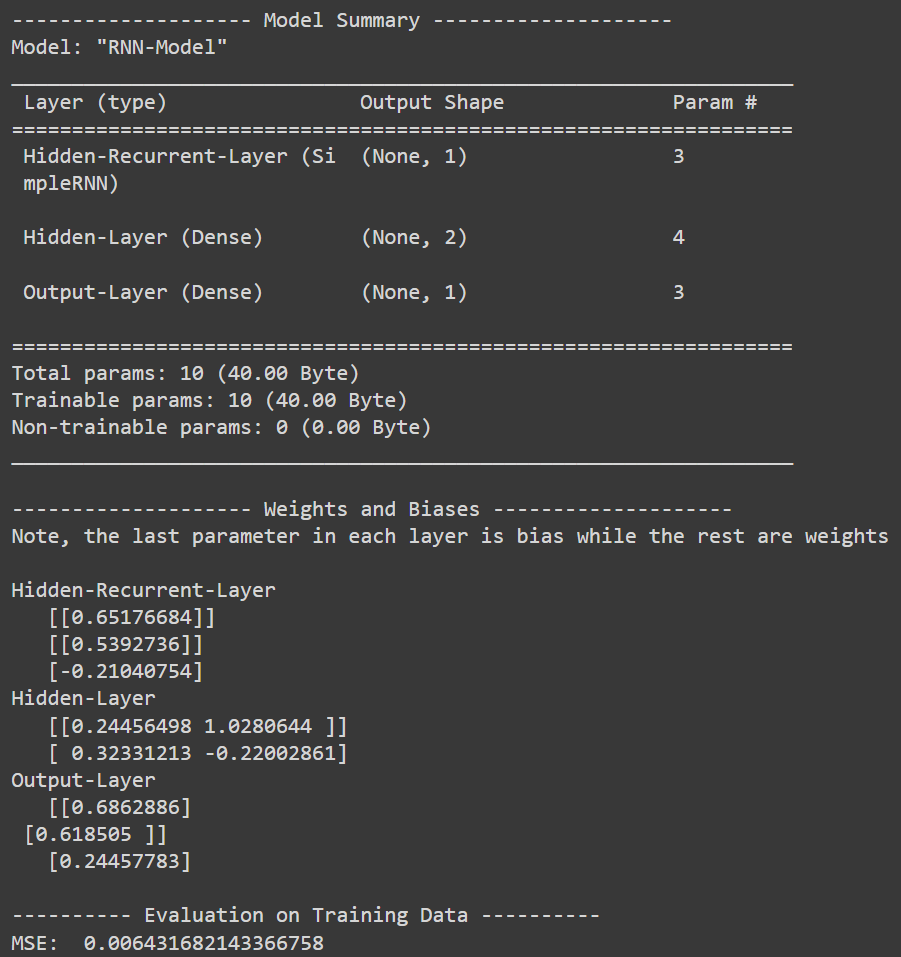
\includegraphics[keepaspectratio]{imagenes/capitulo1/redes_recurrentes/summary_model_rrn.png}}

}

\caption{Summary de la red RRN}

\end{figure}%

\begin{Shaded}
\begin{Highlighting}[numbers=left,,]
\NormalTok{fig }\OperatorTok{=}\NormalTok{ go.Figure()}
\NormalTok{fig.add\_trace(go.Scatter(x}\OperatorTok{=}\NormalTok{np.array(}\BuiltInTok{range}\NormalTok{(}\DecValTok{0}\NormalTok{,}\BuiltInTok{len}\NormalTok{(y\_test))),}
\NormalTok{                         y}\OperatorTok{=}\NormalTok{scaler.inverse\_transform(y\_test).flatten(),}
\NormalTok{                         mode}\OperatorTok{=}\StringTok{\textquotesingle{}lines\textquotesingle{}}\NormalTok{,}
\NormalTok{                         name}\OperatorTok{=}\StringTok{\textquotesingle{}Median Temperature {-} Actual (Test)\textquotesingle{}}\NormalTok{,}
\NormalTok{                         opacity}\OperatorTok{=}\FloatTok{0.8}\NormalTok{,}
\NormalTok{                         line}\OperatorTok{=}\BuiltInTok{dict}\NormalTok{(color}\OperatorTok{=}\StringTok{\textquotesingle{}black\textquotesingle{}}\NormalTok{, width}\OperatorTok{=}\DecValTok{1}\NormalTok{)}
\NormalTok{                        ))}
\NormalTok{fig.add\_trace(go.Scatter(x}\OperatorTok{=}\NormalTok{np.array(}\BuiltInTok{range}\NormalTok{(}\DecValTok{0}\NormalTok{,}\BuiltInTok{len}\NormalTok{(pred\_test))),}
\NormalTok{                         y}\OperatorTok{=}\NormalTok{scaler.inverse\_transform(pred\_test).flatten(),}
\NormalTok{                         mode}\OperatorTok{=}\StringTok{\textquotesingle{}lines\textquotesingle{}}\NormalTok{,}
\NormalTok{                         name}\OperatorTok{=}\StringTok{\textquotesingle{}Median Temperature {-} Predicted (Test)\textquotesingle{}}\NormalTok{,}
\NormalTok{                         opacity}\OperatorTok{=}\FloatTok{0.8}\NormalTok{,}
\NormalTok{                         line}\OperatorTok{=}\BuiltInTok{dict}\NormalTok{(color}\OperatorTok{=}\StringTok{\textquotesingle{}red\textquotesingle{}}\NormalTok{, width}\OperatorTok{=}\DecValTok{1}\NormalTok{)}
\NormalTok{                        ))}

\CommentTok{\# Update axes lines}
\NormalTok{fig.update\_xaxes(showgrid}\OperatorTok{=}\VariableTok{True}\NormalTok{, gridwidth}\OperatorTok{=}\DecValTok{1}\NormalTok{, gridcolor}\OperatorTok{=}\StringTok{\textquotesingle{}lightgrey\textquotesingle{}}\NormalTok{,}
\NormalTok{                 zeroline}\OperatorTok{=}\VariableTok{True}\NormalTok{, zerolinewidth}\OperatorTok{=}\DecValTok{1}\NormalTok{, zerolinecolor}\OperatorTok{=}\StringTok{\textquotesingle{}lightgrey\textquotesingle{}}\NormalTok{,}
\NormalTok{                 showline}\OperatorTok{=}\VariableTok{True}\NormalTok{, linewidth}\OperatorTok{=}\DecValTok{1}\NormalTok{, linecolor}\OperatorTok{=}\StringTok{\textquotesingle{}black\textquotesingle{}}\NormalTok{,}
\NormalTok{                 title}\OperatorTok{=}\StringTok{\textquotesingle{}Observation\textquotesingle{}}
\NormalTok{                )}

\NormalTok{fig.update\_yaxes(showgrid}\OperatorTok{=}\VariableTok{True}\NormalTok{, gridwidth}\OperatorTok{=}\DecValTok{1}\NormalTok{, gridcolor}\OperatorTok{=}\StringTok{\textquotesingle{}lightgrey\textquotesingle{}}\NormalTok{,}
\NormalTok{                 zeroline}\OperatorTok{=}\VariableTok{True}\NormalTok{, zerolinewidth}\OperatorTok{=}\DecValTok{1}\NormalTok{, zerolinecolor}\OperatorTok{=}\StringTok{\textquotesingle{}lightgrey\textquotesingle{}}\NormalTok{,}
\NormalTok{                 showline}\OperatorTok{=}\VariableTok{True}\NormalTok{, linewidth}\OperatorTok{=}\DecValTok{1}\NormalTok{, linecolor}\OperatorTok{=}\StringTok{\textquotesingle{}black\textquotesingle{}}\NormalTok{,}
\NormalTok{                 title}\OperatorTok{=}\StringTok{\textquotesingle{}Degrees Celsius\textquotesingle{}}
\NormalTok{                )}

\CommentTok{\# Set figure title}
\NormalTok{fig.update\_layout(title}\OperatorTok{=}\BuiltInTok{dict}\NormalTok{(text}\OperatorTok{=}\StringTok{"Median Daily Temperatures in Canberra"}\NormalTok{,}
\NormalTok{                             font}\OperatorTok{=}\BuiltInTok{dict}\NormalTok{(color}\OperatorTok{=}\StringTok{\textquotesingle{}black\textquotesingle{}}\NormalTok{)),}
\NormalTok{                  legend}\OperatorTok{=}\BuiltInTok{dict}\NormalTok{(orientation}\OperatorTok{=}\StringTok{"h"}\NormalTok{, yanchor}\OperatorTok{=}\StringTok{"bottom"}\NormalTok{, y}\OperatorTok{=}\FloatTok{1.02}\NormalTok{, xanchor}\OperatorTok{=}\StringTok{"right"}\NormalTok{, x}\OperatorTok{=}\DecValTok{1}\NormalTok{)}
\NormalTok{                 )}

\NormalTok{fig.show()}
\end{Highlighting}
\end{Shaded}

\begin{figure}[H]

{\centering \pandocbounded{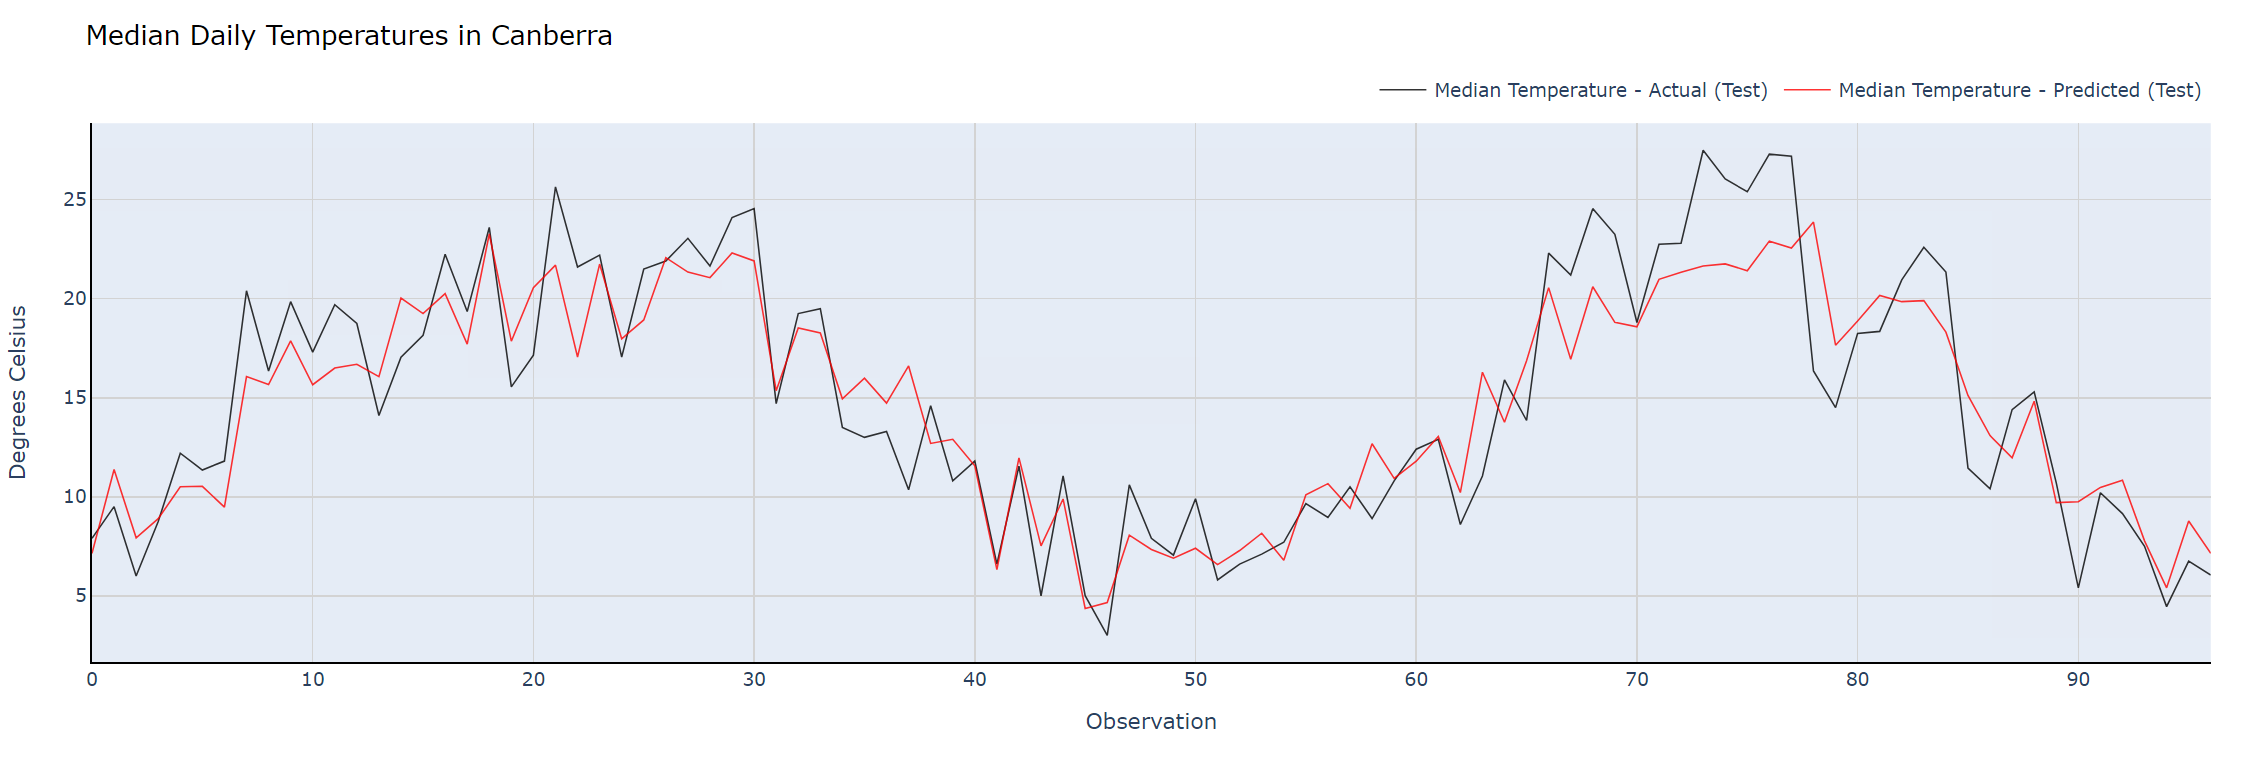
\includegraphics[keepaspectratio]{imagenes/capitulo1/redes_recurrentes/serie_temporal_forecast_1.png}}

}

\caption{Serie temporal con predicciones de la red RRN}

\end{figure}%

En la gráfica podemos ver que el modelo hace unas buenas predicciones,
pero recordemos que el horizonte a predecir es de un día, no es que
nuestro modelo haya podido predecir a 90 días vista.

\textbf{Pregunta:} ¿Qué pasará si intentamos predecir horizontes de
tiempo mayores?

Vamos ahora a usar un modelo LSTM

\begin{Shaded}
\begin{Highlighting}[numbers=left,,]

\CommentTok{\#\#\#\#\# Step 3 {-} Specify the structure of a Neural Network}
\NormalTok{model }\OperatorTok{=}\NormalTok{ Sequential(name}\OperatorTok{=}\StringTok{"LSTM{-}Model"}\NormalTok{) }\CommentTok{\# Model}
\NormalTok{model.add(Input(shape}\OperatorTok{=}\NormalTok{(X\_train.shape[}\DecValTok{1}\NormalTok{],}\DecValTok{1}\NormalTok{), name}\OperatorTok{=}\StringTok{\textquotesingle{}Input{-}Layer\textquotesingle{}}\NormalTok{)) }\CommentTok{\# Input Layer}
\NormalTok{model.add(LSTM(units}\OperatorTok{=}\DecValTok{1}\NormalTok{, activation}\OperatorTok{=}\StringTok{\textquotesingle{}tanh\textquotesingle{}}\NormalTok{, recurrent\_activation}\OperatorTok{=}\StringTok{\textquotesingle{}sigmoid\textquotesingle{}}\NormalTok{, stateful}\OperatorTok{=}\VariableTok{False}\NormalTok{, name}\OperatorTok{=}\StringTok{\textquotesingle{}Hidden{-}LSTM{-}Encoder{-}Layer\textquotesingle{}}\NormalTok{)) }\CommentTok{\# LSTM layer}
\NormalTok{model.add(Dense(units}\OperatorTok{=}\DecValTok{2}\NormalTok{, activation}\OperatorTok{=}\StringTok{\textquotesingle{}tanh\textquotesingle{}}\NormalTok{, name}\OperatorTok{=}\StringTok{\textquotesingle{}Hidden{-}Layer\textquotesingle{}}\NormalTok{)) }\CommentTok{\# Hidden Layer}
\NormalTok{model.add(Dense(units}\OperatorTok{=}\DecValTok{1}\NormalTok{, activation}\OperatorTok{=}\StringTok{\textquotesingle{}linear\textquotesingle{}}\NormalTok{, name}\OperatorTok{=}\StringTok{\textquotesingle{}Output{-}Layer\textquotesingle{}}\NormalTok{)) }\CommentTok{\# Output Layer, Linear(x) = x}


\CommentTok{\#\#\#\#\# Step 4 {-} Compile the model}
\NormalTok{model.}\BuiltInTok{compile}\NormalTok{(}
\NormalTok{    optimizer}\OperatorTok{=}\StringTok{\textquotesingle{}adam\textquotesingle{}}\NormalTok{, }\CommentTok{\# default=\textquotesingle{}rmsprop\textquotesingle{}, an algorithm to be used in backpropagation}
\NormalTok{    loss}\OperatorTok{=}\StringTok{\textquotesingle{}mean\_squared\_error\textquotesingle{}}\NormalTok{, }\CommentTok{\# Loss function to be optimized. A string (name of loss function), or a tf.keras.losses.Loss instance.}
\NormalTok{    metrics}\OperatorTok{=}\NormalTok{[}\StringTok{\textquotesingle{}MeanSquaredError\textquotesingle{}}\NormalTok{, }\StringTok{\textquotesingle{}MeanAbsoluteError\textquotesingle{}}\NormalTok{], }\CommentTok{\# List of metrics to be evaluated by the model during training and testing. Each of this can be a string (name of a built{-}in function), function or a tf.keras.metrics.Metric instance.}
\NormalTok{    loss\_weights}\OperatorTok{=}\VariableTok{None}\NormalTok{, }\CommentTok{\# default=None, Optional list or dictionary specifying scalar coefficients (Python floats) to weight the loss contributions of different model outputs.}
\NormalTok{    weighted\_metrics}\OperatorTok{=}\VariableTok{None}\NormalTok{, }\CommentTok{\# default=None, List of metrics to be evaluated and weighted by sample\_weight or class\_weight during training and testing.}
\NormalTok{    run\_eagerly}\OperatorTok{=}\VariableTok{None} \CommentTok{\# Defaults to False. If True, this Model\textquotesingle{}s logic will not be wrapped in a tf.function. Recommended to leave this as None unless your Model cannot be run inside a tf.function.}
\NormalTok{   )}

\CommentTok{\# \#\#\#\#\# Step 6 {-} Fit keras model on the dataset}
\NormalTok{model.fit(}
\NormalTok{    X\_train, }\CommentTok{\# input data}
\NormalTok{    y\_train, }\CommentTok{\# target data}
\NormalTok{    batch\_size}\OperatorTok{=}\DecValTok{1}\NormalTok{, }\CommentTok{\# Number of samples per gradient update.}
\NormalTok{    epochs}\OperatorTok{=}\DecValTok{20}\NormalTok{, }\CommentTok{\# default=1, Number of epochs to train the model}
\NormalTok{    validation\_split}\OperatorTok{=}\FloatTok{0.0}\NormalTok{, }\CommentTok{\# default=0.0, Fraction of the training data to be used as validation data. The model will set apart this fraction of the training data, will not train on it, and will evaluate the loss and any model metrics on this data at the end of each epoch.}
    \CommentTok{\#validation\_data=(X\_test, y\_test), \# default=None, Data on which to evaluate the loss and any model metrics at the end of each epoch.}
\NormalTok{    shuffle}\OperatorTok{=}\VariableTok{True}\NormalTok{, }\CommentTok{\# default=True, Boolean (whether to shuffle the training data before each epoch) or str (for \textquotesingle{}batch\textquotesingle{}).}
\NormalTok{    class\_weight}\OperatorTok{=}\VariableTok{None}\NormalTok{, }\CommentTok{\# default=None, Optional dictionary mapping class indices (integers) to a weight (float) value, used for weighting the loss function (during training only). This can be useful to tell the model to "pay more attention" to samples from an under{-}represented class.}
\NormalTok{    sample\_weight}\OperatorTok{=}\VariableTok{None}\NormalTok{, }\CommentTok{\# default=None, Optional Numpy array of weights for the training samples, used for weighting the loss function (during training only).}
\NormalTok{    initial\_epoch}\OperatorTok{=}\DecValTok{0}\NormalTok{, }\CommentTok{\# Integer, default=0, Epoch at which to start training (useful for resuming a previous training run).}
\NormalTok{    steps\_per\_epoch}\OperatorTok{=}\VariableTok{None}\NormalTok{, }\CommentTok{\# Integer or None, default=None, Total number of steps (batches of samples) before declaring one epoch finished and starting the next epoch. When training with input tensors such as TensorFlow data tensors, the default None is equal to the number of samples in your dataset divided by the batch size, or 1 if that cannot be determined.}
\NormalTok{    validation\_steps}\OperatorTok{=}\VariableTok{None}\NormalTok{, }\CommentTok{\# Only relevant if validation\_data is provided and is a tf.data dataset. Total number of steps (batches of samples) to draw before stopping when performing validation at the end of every epoch.}
\NormalTok{    validation\_batch\_size}\OperatorTok{=}\VariableTok{None}\NormalTok{, }\CommentTok{\# Integer or None, default=None, Number of samples per validation batch. If unspecified, will default to batch\_size.}
\NormalTok{    validation\_freq}\OperatorTok{=}\DecValTok{1} \CommentTok{\# default=1, Only relevant if validation data is provided. If an integer, specifies how many training epochs to run before a new validation run is performed, e.g. validation\_freq=2 runs validation every 2 epochs.}
\NormalTok{)}


\CommentTok{\#\#\#\#\# Step 7 {-} Make predictions}
\CommentTok{\# Predict the result on training data}
\NormalTok{pred\_train\_lstm }\OperatorTok{=}\NormalTok{ model.predict(X\_train)}
\CommentTok{\# Predict the result on test data}
\NormalTok{pred\_test\_lstm }\OperatorTok{=}\NormalTok{ model.predict(X\_test)}


\CommentTok{\#\#\#\#\# Step 8 {-} Model Performance Summary}
\BuiltInTok{print}\NormalTok{(}\StringTok{""}\NormalTok{)}
\BuiltInTok{print}\NormalTok{(}\StringTok{\textquotesingle{}{-}{-}{-}{-}{-}{-}{-}{-}{-}{-}{-}{-}{-}{-}{-}{-}{-}{-}{-}{-} Model Summary {-}{-}{-}{-}{-}{-}{-}{-}{-}{-}{-}{-}{-}{-}{-}{-}{-}{-}{-}{-}\textquotesingle{}}\NormalTok{)}
\NormalTok{model.summary() }\CommentTok{\# print model summary}
\BuiltInTok{print}\NormalTok{(}\StringTok{""}\NormalTok{)}
\BuiltInTok{print}\NormalTok{(}\StringTok{\textquotesingle{}{-}{-}{-}{-}{-}{-}{-}{-}{-}{-}{-}{-}{-}{-}{-}{-}{-}{-}{-}{-} Weights and Biases {-}{-}{-}{-}{-}{-}{-}{-}{-}{-}{-}{-}{-}{-}{-}{-}{-}{-}{-}{-}\textquotesingle{}}\NormalTok{)}
\BuiltInTok{print}\NormalTok{(}\StringTok{"Note, the last parameter in each layer is bias while the rest are weights"}\NormalTok{)}
\BuiltInTok{print}\NormalTok{(}\StringTok{""}\NormalTok{)}
\ControlFlowTok{for}\NormalTok{ layer }\KeywordTok{in}\NormalTok{ model.layers:}
    \BuiltInTok{print}\NormalTok{(layer.name)}
    \ControlFlowTok{for}\NormalTok{ item }\KeywordTok{in}\NormalTok{ layer.get\_weights():}
        \BuiltInTok{print}\NormalTok{(}\StringTok{"  "}\NormalTok{, item)}
\BuiltInTok{print}\NormalTok{(}\StringTok{""}\NormalTok{)}
\BuiltInTok{print}\NormalTok{(}\StringTok{\textquotesingle{}{-}{-}{-}{-}{-}{-}{-}{-}{-}{-} Evaluation on Training Data {-}{-}{-}{-}{-}{-}{-}{-}{-}{-}\textquotesingle{}}\NormalTok{)}
\BuiltInTok{print}\NormalTok{(}\StringTok{"MSE: "}\NormalTok{, mean\_squared\_error(y\_train, pred\_train\_lstm))}
\BuiltInTok{print}\NormalTok{(}\StringTok{""}\NormalTok{)}

\BuiltInTok{print}\NormalTok{(}\StringTok{\textquotesingle{}{-}{-}{-}{-}{-}{-}{-}{-}{-}{-} Evaluation on Test Data {-}{-}{-}{-}{-}{-}{-}{-}{-}{-}\textquotesingle{}}\NormalTok{)}
\BuiltInTok{print}\NormalTok{(}\StringTok{"MSE: "}\NormalTok{, mean\_squared\_error(y\_test, pred\_test\_lstm))}
\BuiltInTok{print}\NormalTok{(}\StringTok{""}\NormalTok{)}
\end{Highlighting}
\end{Shaded}

\begin{figure}[H]

{\centering \pandocbounded{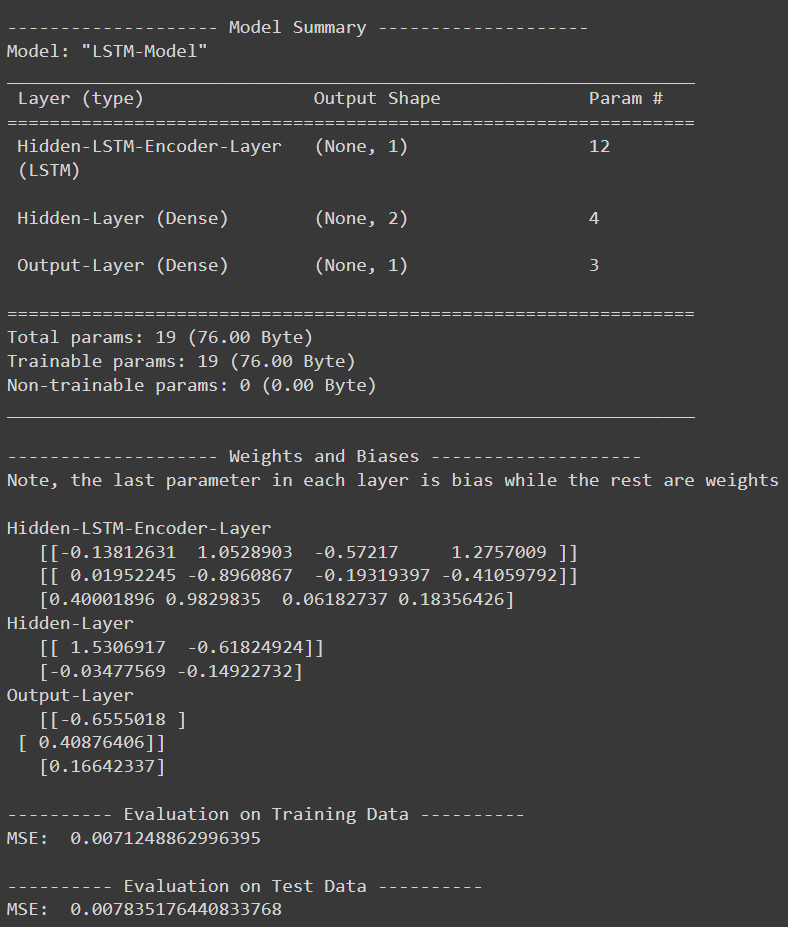
\includegraphics[keepaspectratio]{imagenes/capitulo1/redes_recurrentes/summary_model_lstm.png}}

}

\caption{Summary red LSTM}

\end{figure}%

\begin{Shaded}
\begin{Highlighting}[numbers=left,,]
\NormalTok{fig }\OperatorTok{=}\NormalTok{ go.Figure()}
\NormalTok{fig.add\_trace(go.Scatter(x}\OperatorTok{=}\NormalTok{np.array(}\BuiltInTok{range}\NormalTok{(}\DecValTok{0}\NormalTok{,}\BuiltInTok{len}\NormalTok{(y\_test))),}
\NormalTok{                         y}\OperatorTok{=}\NormalTok{scaler.inverse\_transform(y\_test).flatten(),}
\NormalTok{                         mode}\OperatorTok{=}\StringTok{\textquotesingle{}lines\textquotesingle{}}\NormalTok{,}
\NormalTok{                         name}\OperatorTok{=}\StringTok{\textquotesingle{}Median Temperature {-} Actual (Test)\textquotesingle{}}\NormalTok{,}
\NormalTok{                         opacity}\OperatorTok{=}\FloatTok{0.8}\NormalTok{,}
\NormalTok{                         line}\OperatorTok{=}\BuiltInTok{dict}\NormalTok{(color}\OperatorTok{=}\StringTok{\textquotesingle{}black\textquotesingle{}}\NormalTok{, width}\OperatorTok{=}\DecValTok{1}\NormalTok{)}
\NormalTok{                        ))}

\NormalTok{fig.add\_trace(go.Scatter(x}\OperatorTok{=}\NormalTok{np.array(}\BuiltInTok{range}\NormalTok{(}\DecValTok{0}\NormalTok{,}\BuiltInTok{len}\NormalTok{(pred\_test))),}
\NormalTok{                         y}\OperatorTok{=}\NormalTok{scaler.inverse\_transform(pred\_test).flatten(),}
\NormalTok{                         mode}\OperatorTok{=}\StringTok{\textquotesingle{}lines\textquotesingle{}}\NormalTok{,}
\NormalTok{                         name}\OperatorTok{=}\StringTok{\textquotesingle{}Median Temperature {-} RRN Predicted (Test)\textquotesingle{}}\NormalTok{,}
\NormalTok{                         opacity}\OperatorTok{=}\FloatTok{0.8}\NormalTok{,}
\NormalTok{                         line}\OperatorTok{=}\BuiltInTok{dict}\NormalTok{(color}\OperatorTok{=}\StringTok{\textquotesingle{}red\textquotesingle{}}\NormalTok{, width}\OperatorTok{=}\DecValTok{1}\NormalTok{)}
\NormalTok{                        ))}

\NormalTok{fig.add\_trace(go.Scatter(x}\OperatorTok{=}\NormalTok{np.array(}\BuiltInTok{range}\NormalTok{(}\DecValTok{0}\NormalTok{,}\BuiltInTok{len}\NormalTok{(pred\_test\_lstm))),}
\NormalTok{                         y}\OperatorTok{=}\NormalTok{scaler.inverse\_transform(pred\_test\_lstm).flatten(),}
\NormalTok{                         mode}\OperatorTok{=}\StringTok{\textquotesingle{}lines\textquotesingle{}}\NormalTok{,}
\NormalTok{                         name}\OperatorTok{=}\StringTok{\textquotesingle{}Median Temperature {-} LSTM Predicted (Test)\textquotesingle{}}\NormalTok{,}
\NormalTok{                         opacity}\OperatorTok{=}\FloatTok{0.8}\NormalTok{,}
\NormalTok{                         line}\OperatorTok{=}\BuiltInTok{dict}\NormalTok{(color}\OperatorTok{=}\StringTok{\textquotesingle{}blue\textquotesingle{}}\NormalTok{, width}\OperatorTok{=}\DecValTok{1}\NormalTok{)}
\NormalTok{                        ))}

\CommentTok{\# Update axes lines}
\NormalTok{fig.update\_xaxes(showgrid}\OperatorTok{=}\VariableTok{True}\NormalTok{, gridwidth}\OperatorTok{=}\DecValTok{1}\NormalTok{, gridcolor}\OperatorTok{=}\StringTok{\textquotesingle{}lightgrey\textquotesingle{}}\NormalTok{,}
\NormalTok{                 zeroline}\OperatorTok{=}\VariableTok{True}\NormalTok{, zerolinewidth}\OperatorTok{=}\DecValTok{1}\NormalTok{, zerolinecolor}\OperatorTok{=}\StringTok{\textquotesingle{}lightgrey\textquotesingle{}}\NormalTok{,}
\NormalTok{                 showline}\OperatorTok{=}\VariableTok{True}\NormalTok{, linewidth}\OperatorTok{=}\DecValTok{1}\NormalTok{, linecolor}\OperatorTok{=}\StringTok{\textquotesingle{}black\textquotesingle{}}\NormalTok{,}
\NormalTok{                 title}\OperatorTok{=}\StringTok{\textquotesingle{}Observation\textquotesingle{}}
\NormalTok{                )}

\NormalTok{fig.update\_yaxes(showgrid}\OperatorTok{=}\VariableTok{True}\NormalTok{, gridwidth}\OperatorTok{=}\DecValTok{1}\NormalTok{, gridcolor}\OperatorTok{=}\StringTok{\textquotesingle{}lightgrey\textquotesingle{}}\NormalTok{,}
\NormalTok{                 zeroline}\OperatorTok{=}\VariableTok{True}\NormalTok{, zerolinewidth}\OperatorTok{=}\DecValTok{1}\NormalTok{, zerolinecolor}\OperatorTok{=}\StringTok{\textquotesingle{}lightgrey\textquotesingle{}}\NormalTok{,}
\NormalTok{                 showline}\OperatorTok{=}\VariableTok{True}\NormalTok{, linewidth}\OperatorTok{=}\DecValTok{1}\NormalTok{, linecolor}\OperatorTok{=}\StringTok{\textquotesingle{}black\textquotesingle{}}\NormalTok{,}
\NormalTok{                 title}\OperatorTok{=}\StringTok{\textquotesingle{}Degrees Celsius\textquotesingle{}}
\NormalTok{                )}

\CommentTok{\# Set figure title}
\NormalTok{fig.update\_layout(}
\NormalTok{    title }\OperatorTok{=} \BuiltInTok{dict}\NormalTok{(text}\OperatorTok{=}\StringTok{"Median Daily Temperatures in Canberra"}\NormalTok{, font}\OperatorTok{=}\BuiltInTok{dict}\NormalTok{(color}\OperatorTok{=}\StringTok{\textquotesingle{}black\textquotesingle{}}\NormalTok{)),}
\NormalTok{    legend }\OperatorTok{=} \BuiltInTok{dict}\NormalTok{(orientation}\OperatorTok{=}\StringTok{"h"}\NormalTok{, yanchor}\OperatorTok{=}\StringTok{"bottom"}\NormalTok{, y}\OperatorTok{=}\FloatTok{1.02}\NormalTok{, xanchor}\OperatorTok{=}\StringTok{"right"}\NormalTok{, x}\OperatorTok{=}\DecValTok{1}\NormalTok{)}
\NormalTok{)}

\NormalTok{fig.show()}
\end{Highlighting}
\end{Shaded}

\begin{figure}[H]

{\centering \pandocbounded{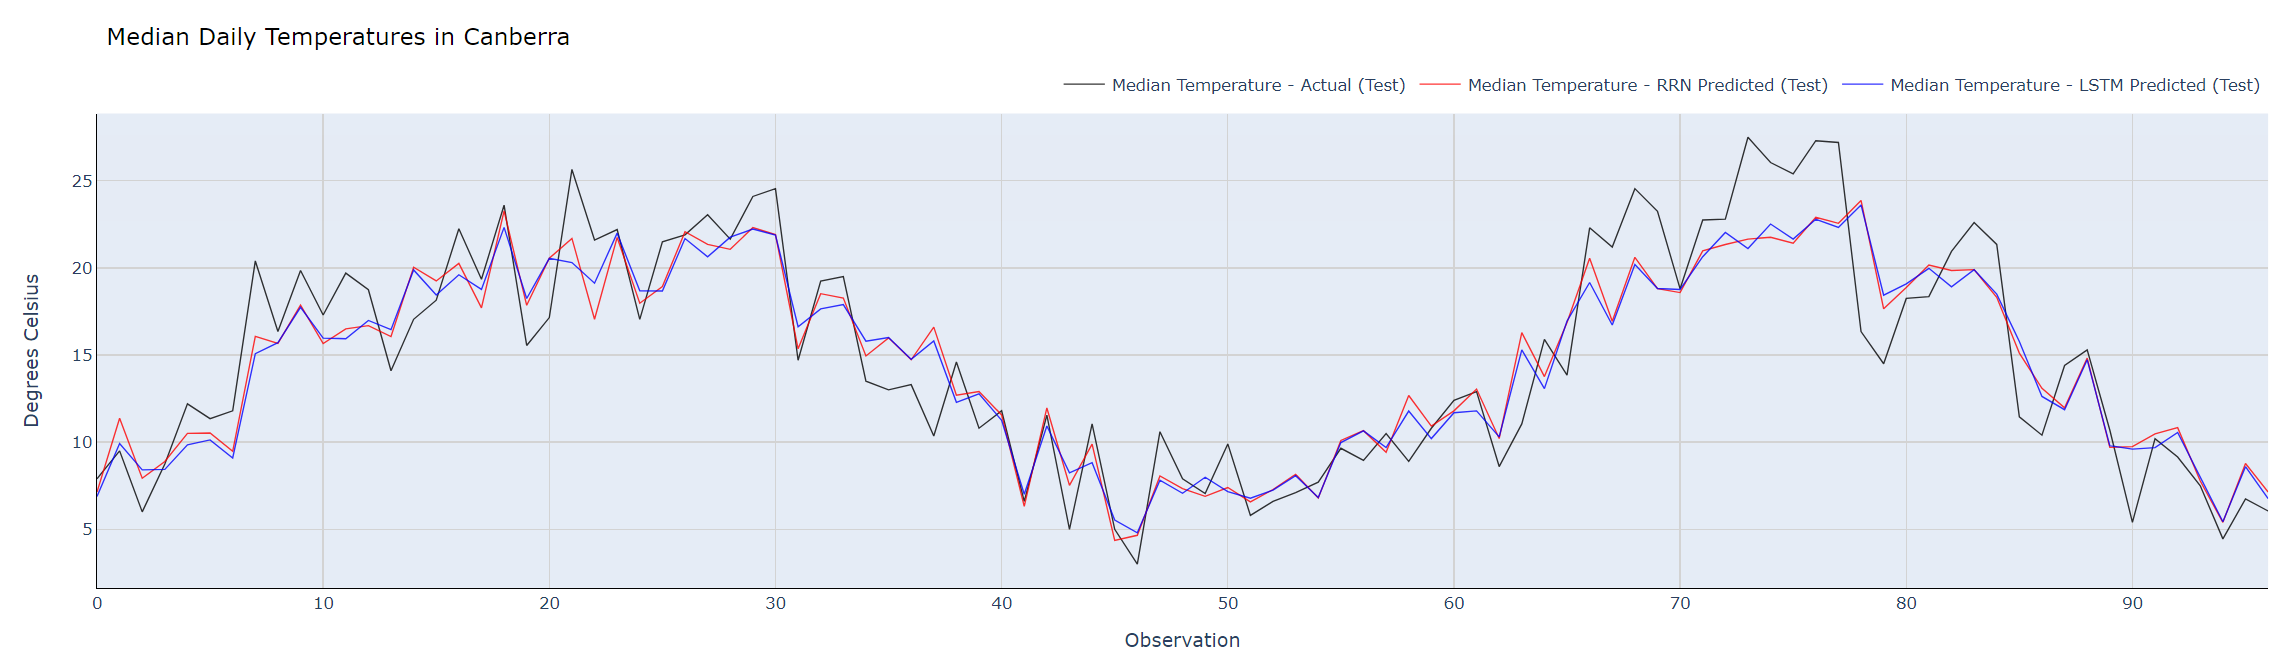
\includegraphics[keepaspectratio]{imagenes/capitulo1/redes_recurrentes/serie_temporal_forecast_2.png}}

}

\caption{Serie temporal con predicciones}

\end{figure}%

Mirando los resultados, parece que nuestro modelo LSTM tiene un
desempeño similar a nuestra RRN, ¿Cómo puede ser?¿Se suponia que la LSTM
era más potente?

Y así es. En este caso no apreciamos diferencias porque el modelo tiene
la información de los 7 días previos y tiene que predecir solo 1 día.
Nuestra RRN es capaz de captar las dependencias entre los datos, por lo
que la LSTM no tiene mucho margen de mejora. Otro asunto sería si
intentasemos predecir un mayor horizonte de tiempo o si usasemos
secuencias más largas. En ese caso, la RRN no podría aprender
dependencias a largo plazo y la LSTM obtendría un mejor resultado.

Podéis probar a variar las condiciones del problema para encontrar
situaciones en las que la LSTM obtenga un mejor desempeño que la RRN.

\textbf{Nota:} Dado que las temperaturas diarias fluctuan mucho, podéis
probar a agregar las temperaturas a nivel semanal / mensual para que la
secuencia sea más estable.

\subsection{Ejemplo: Análisis de
sentimiento}\label{ejemplo-anuxe1lisis-de-sentimiento}

A continuación usaremos una red LSTM para clasificar como positivas o
negativas las reviews de IMDB. Por simplicidad, no trabajaremos con las
reviews directamente, sino que \texttt{Keras} nos ofrece la posibilidad
de cargar las reviews preprocesadas donde cada una de ellas se codifica
como una lista de índices de palabras (números enteros). Para mayor
comodidad, las palabras se indexan por frecuencia global en el conjunto
de datos, de modo que, por ejemplo, el entero ``3'' codifica la 3ª
palabra más frecuente en los datos. Esto permite realizar rápidamente
operaciones de filtrado como: ``considerar sólo las 10.000 palabras más
frecuentes, pero eliminar las 20 palabras más frecuentes''. En este caso
nosotros usaremos un vocabulario de 6000 palabras.

\begin{Shaded}
\begin{Highlighting}[numbers=left,,]

\ImportTok{from}\NormalTok{ tensorflow.keras.datasets }\ImportTok{import}\NormalTok{ imdb}
\CommentTok{\# load the dataset but only keep the top n words, zero the rest}
\NormalTok{vocabulary\_size }\OperatorTok{=} \DecValTok{6000}
\NormalTok{(X\_train, y\_train), (X\_test, y\_test) }\OperatorTok{=}\NormalTok{ imdb.load\_data(num\_words}\OperatorTok{=}\NormalTok{vocabulary\_size)}
\BuiltInTok{print}\NormalTok{ (}\SpecialStringTok{f"Loaded dataset with }\SpecialCharTok{\{}\BuiltInTok{len}\NormalTok{(X\_train)}\SpecialCharTok{\}}\SpecialStringTok{ training sampmles, }\SpecialCharTok{\{}\BuiltInTok{len}\NormalTok{(X\_test)}\SpecialCharTok{\}}\SpecialStringTok{ test samples"}\NormalTok{)}
\end{Highlighting}
\end{Shaded}

Una vez generadas nuestras tuplas con los datos de entrenamiento, las
etiquetas de entrenamiento y la parte de test correspondiente, podemos
visualizarlo:

\begin{Shaded}
\begin{Highlighting}[numbers=left,,]
\BuiltInTok{print}\NormalTok{ (}\StringTok{" {-} {-} {-} Review {-} {-} {-} "}\NormalTok{)}
\BuiltInTok{print}\NormalTok{ (X\_train [}\DecValTok{0}\NormalTok{])}
\BuiltInTok{print}\NormalTok{ (}\StringTok{" {-} {-} {-} Label {-} {-} {-} "}\NormalTok{)}
\BuiltInTok{print}\NormalTok{ (y\_train [}\DecValTok{0}\NormalTok{])}

\NormalTok{word2id }\OperatorTok{=}\NormalTok{ imdb.get\_word\_index()}
\NormalTok{id2word }\OperatorTok{=}\NormalTok{ \{i: word }\ControlFlowTok{for}\NormalTok{ word, i }\KeywordTok{in}\NormalTok{ word2id.items()\}}
\BuiltInTok{print}\NormalTok{ (}\StringTok{" {-} {-} {-} Review (with words) {-} {-} {-} "}\NormalTok{)}
\BuiltInTok{print}\NormalTok{ ([id2word.get (i, }\StringTok{"  "}\NormalTok{) }\ControlFlowTok{for}\NormalTok{ i }\KeywordTok{in}\NormalTok{ X\_train[}\DecValTok{0}\NormalTok{]])}
\BuiltInTok{print}\NormalTok{ (}\StringTok{" {-} {-} {-} Label {-} {-} {-} "}\NormalTok{)}
\BuiltInTok{print}\NormalTok{ (y\_train [}\DecValTok{0}\NormalTok{])}
\end{Highlighting}
\end{Shaded}

\begin{figure}[H]

{\centering \pandocbounded{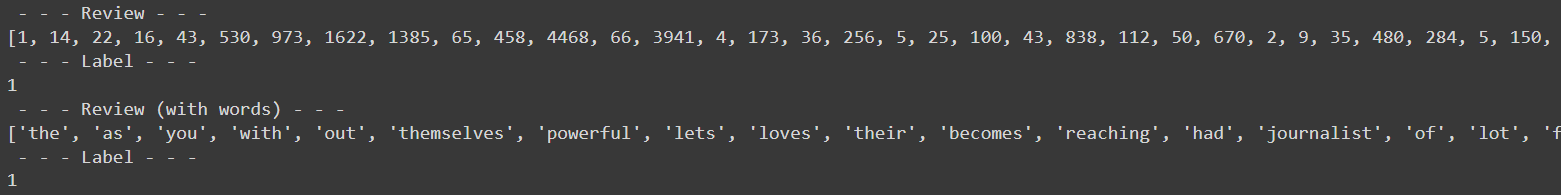
\includegraphics[keepaspectratio]{imagenes/capitulo1/redes_recurrentes/reviews.png}}

}

\caption{Reviews}

\end{figure}%

Con esto ya tendríamos los datos tokenizados con las etiquetas. Ahora ya
podemos pasarle las reviews a la red. Para ello, lo primero será definir
el tamaño de entrada de la red. En este caso utilizaremos un tamaño de
500, lo que quiere decir que los datos de entrada para la predicción y
análisis de sentimientos son 500 palabras.

\begin{Shaded}
\begin{Highlighting}[numbers=left,,]
\NormalTok{max\_words }\OperatorTok{=} \DecValTok{500}
\NormalTok{X\_train }\OperatorTok{=}\NormalTok{ pad\_sequences(X\_train, maxlen }\OperatorTok{=}\NormalTok{ max\_words)}
\NormalTok{X\_test }\OperatorTok{=}\NormalTok{ pad\_sequences(X\_test, maxlen }\OperatorTok{=}\NormalTok{ max\_words)}
\end{Highlighting}
\end{Shaded}

Ahora crearemos el modelo:

\begin{Shaded}
\begin{Highlighting}[numbers=left,,]

\NormalTok{model }\OperatorTok{=}\NormalTok{ Sequential ()}
\NormalTok{model.add (Embedding(vocabulary\_size, }\DecValTok{128}\NormalTok{, input\_length }\OperatorTok{=}\NormalTok{ max\_words))}
\NormalTok{model.add(Bidirectional(LSTM(units}\OperatorTok{=}\DecValTok{64}\NormalTok{, activation}\OperatorTok{=}\StringTok{\textquotesingle{}tanh\textquotesingle{}}\NormalTok{, return\_sequences}\OperatorTok{=}\VariableTok{True}\NormalTok{), name}\OperatorTok{=}\StringTok{\textquotesingle{}Hidden{-}LSTM{-}Encoder{-}Layer\textquotesingle{}}\NormalTok{)) }\CommentTok{\# Encoder Layer}
\NormalTok{model.add(Bidirectional(LSTM(units}\OperatorTok{=}\DecValTok{64}\NormalTok{, activation}\OperatorTok{=}\StringTok{\textquotesingle{}tanh\textquotesingle{}}\NormalTok{), name}\OperatorTok{=}\StringTok{\textquotesingle{}Hidden{-}LSTM{-}Decoder{-}Layer\textquotesingle{}}\NormalTok{)) }\CommentTok{\# Encoder Layer}
\NormalTok{model.add (Dense (}\DecValTok{1}\NormalTok{, activation }\OperatorTok{=} \StringTok{\textquotesingle{}sigmoid\textquotesingle{}}\NormalTok{))}

\NormalTok{model.}\BuiltInTok{compile}\NormalTok{ (loss }\OperatorTok{=} \StringTok{\textquotesingle{}binary\_crossentropy\textquotesingle{}}\NormalTok{, optimizer }\OperatorTok{=} \StringTok{\textquotesingle{}adam\textquotesingle{}}\NormalTok{, metrics }\OperatorTok{=}\NormalTok{ [}\StringTok{\textquotesingle{}accuracy\textquotesingle{}}\NormalTok{])}

\NormalTok{model.fit(X\_train, y\_train, batch\_size}\OperatorTok{=}\DecValTok{32}\NormalTok{, epochs}\OperatorTok{=}\DecValTok{2}\NormalTok{, validation\_split}\OperatorTok{=}\FloatTok{0.1}\NormalTok{)}
\end{Highlighting}
\end{Shaded}

Con el siguiente comando nos podemos crear una matriz de confusión
dinamica, en función del threshold que escogamos. Seleccionando
distintos puntos de corte, vemos que nuestro modelo ha obtenido muy
buenos resultados

\begin{Shaded}
\begin{Highlighting}[numbers=left,,]
\NormalTok{pred\_test }\OperatorTok{=}\NormalTok{ model.predict(X\_test)}

\NormalTok{cf\_fig, var\_metrics\_df, invar\_metrics\_df, opt\_thresh\_df }\OperatorTok{=}\NormalTok{ bc.confusion\_matrix\_plot(}
\NormalTok{    true\_y }\OperatorTok{=}\NormalTok{ y\_test,}
\NormalTok{    predicted\_proba }\OperatorTok{=}\NormalTok{ pred\_test,}
\NormalTok{    threshold\_step }\OperatorTok{=} \FloatTok{0.05}\NormalTok{,}
\NormalTok{    title }\OperatorTok{=} \StringTok{\textquotesingle{}Interactive Confusion Matrix for the Test Set\textquotesingle{}}\NormalTok{)}
\NormalTok{cf\_fig}
\end{Highlighting}
\end{Shaded}

\begin{figure}[H]

{\centering \pandocbounded{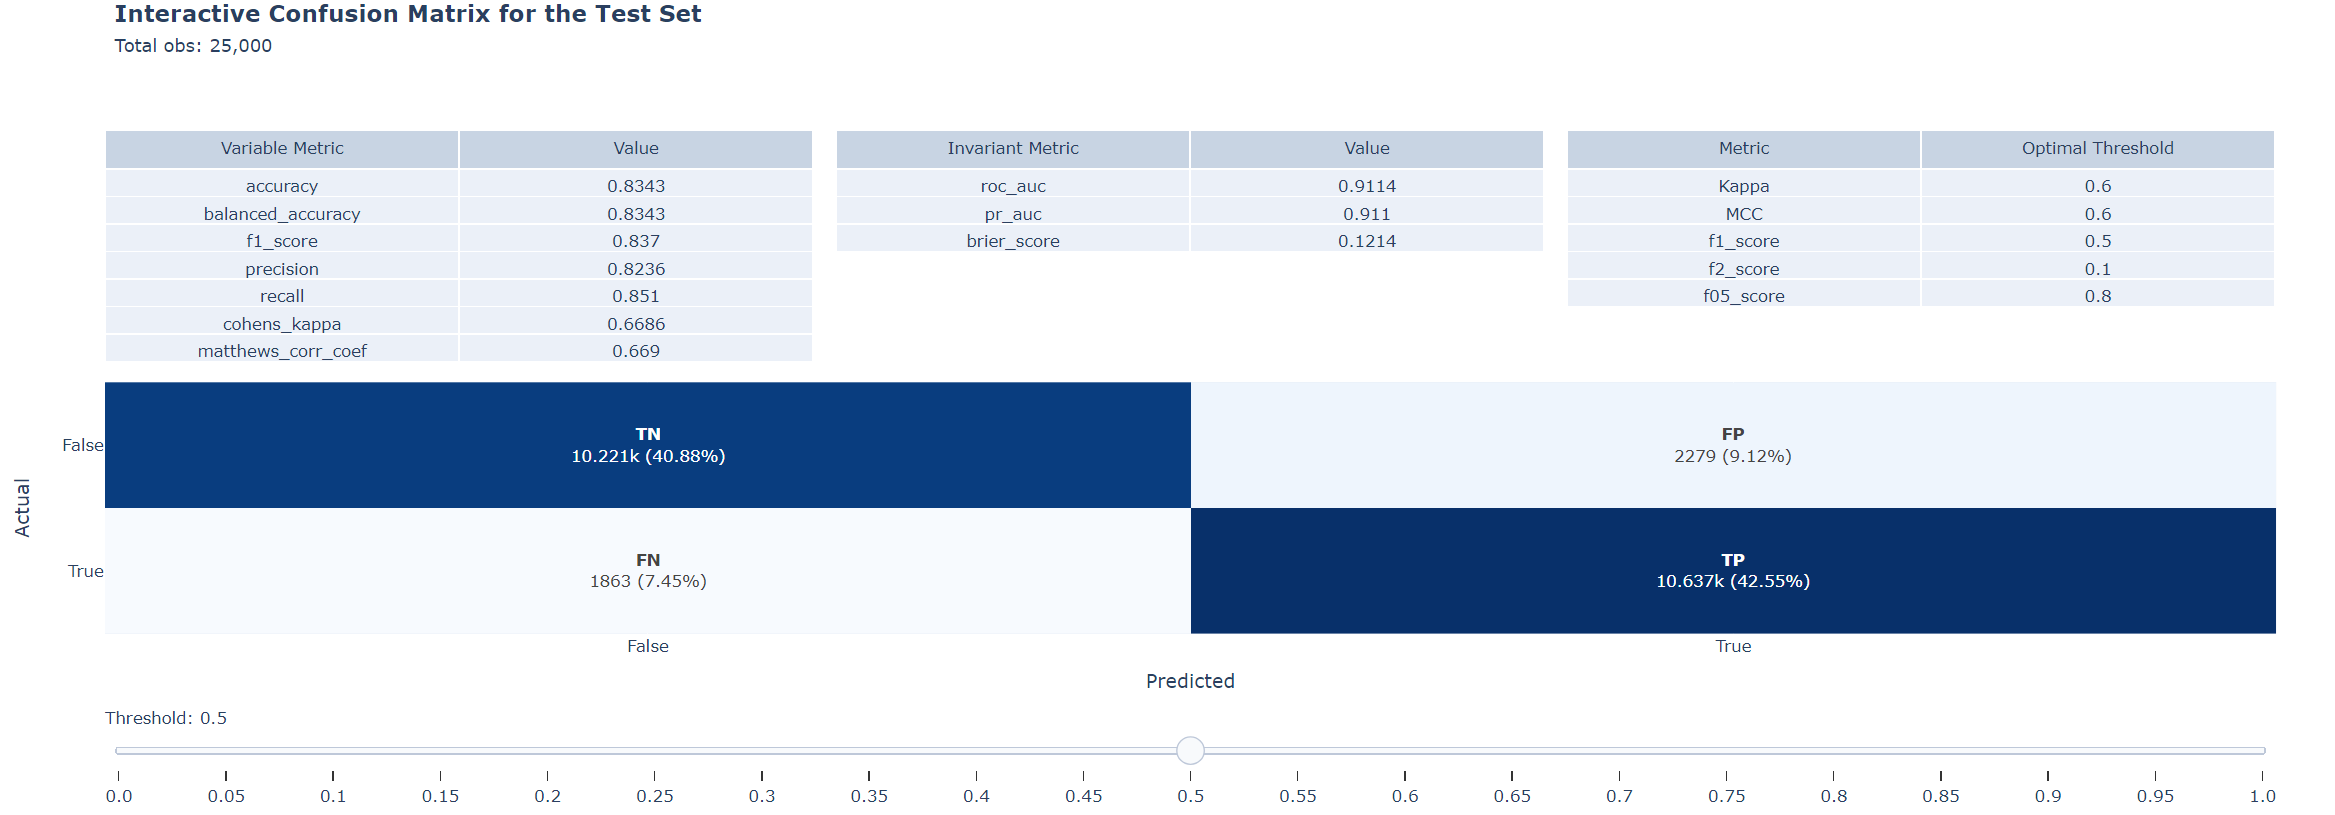
\includegraphics[keepaspectratio]{imagenes/capitulo1/redes_recurrentes/binclass.png}}

}

\caption{Matriz de confusión}

\end{figure}%

\section{Autoencoders}\label{autoencoders}

\subsection{Bases del Autoencoder}\label{bases-del-autoencoder}

Los \textbf{Autoencoders (AE)} son uno de los tipos de redes neuronales
que caen dentro del ámbito del Deep Learning, en la que nos encontramos
con un modelo de \textbf{aprendizaje no supervisado}. Ya se empezó a
hablar de AE en la década de los 80 (Bourlard and Kamp 1988), aunque es
en estos últimos años donde más se está trabajando con ellos.

La arquitectura de un AE es una Red Neuronal Artificial (ANN por sus
siglas en inglés) que se encuentra dividida en dos partes,
\textbf{encoder} y \textbf{decoder} (Charte et al.~2018), (Goodfellow,
Bengio, and Courville 2016). El encoder va a ser la parte de la ANN que
va codificar o comprimir los datos de entrada, y el decoder será el
encargado de regenerar de nuevo los datos en la salida. Esta estructura
de codificación y decodificación le llevará a tener una estructura
simétrica. El AE es entrenado para ser capaz de reconstruir los datos de
entrada en la capa de salida de la ANN, implementando una serie de
restricciones (la reducción de elementos en las capas ocultas del
encoder) que van a evitar que simplemente se copie la entrada en la
salida.

Si recordamos la estructura de una ANN clásica o también llamada
\textbf{Red Neuronal Densamente} \textbf{Conectada} (ya que cada neurona
conecta con todas las de la siguiente capa) nos encontramos en que en
esta arquitectura, generalmente, el número de neuronas por capa se va
reduciendo hasta llegar a la capa de salida que debería ser normalmente
un número (si estamos en un problema regresión), un dato binario (si es
un problema de clasificación).

\begin{figure}

\centering{

\pandocbounded{\includegraphics[keepaspectratio]{imagenes/capitulo1/Redneuronal.png}}

}

\caption{\label{fig-redneuronal}Red Neuronal Clasica}

\end{figure}%

Ya se empezó a hablar de AE en la década de los 80 (Bourlard and Kamp
1988), aunque es en estos últimos años donde más se está trabajando con
ellos.

La arquitectura de un AE es una Red Neuronal Artificial (ANN por sus
siglas en inglés) que se encuentra dividida en dos partes,
\textbf{encoder} y \textbf{decoder} (Charte et al.~2018), (Goodfellow,
Bengio, and Courville 2016). El encoder va a ser la parte de la ANN que
va codificar o comprimir los datos de entrada, y el decoder será el
encargado de regenerar de nuevo los datos en la salida. Esta estructura
de codificación y decodificación le llevará a tener una estructura
simétrica. El AE es entrenado para ser capaz de reconstruir los datos de
entrada en la capa de salida de la ANN, implementando una serie de
restricciones (la reducción de elementos en las capas ocultas del
encoder) que van a evitar que simplemente se copie la entrada en la
salida.

Si recordamos la estructura de una ANN clásica o también llamada
\textbf{Red Neuronal Densamente Conectada} (ya que cada neurona conecta
con todas las de la siguiente capa) nos encontramos en que en esta
arquitectura, generalmente, el número de neuronas por capa se va
reduciendo hasta llegar a la capa de salida que debería ser normalmente
un número (si estamos en un problema regresión), un dato binario (si es
un problema de clasificación).

Si pensamos en una estructura básica de AE en la que tenemos una capa de
entrada, una capa oculta y una capa de salida, ésta sería su
representación:

\begin{figure}

\centering{

\pandocbounded{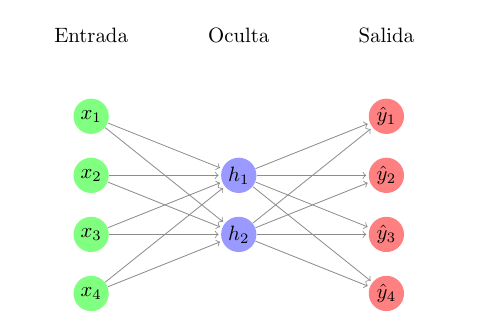
\includegraphics[keepaspectratio]{imagenes/capitulo1/autoencoder_basico.png}}

}

\caption{\label{fig-autoencoder_basico}Autoencoder Básico}

\end{figure}%

Donde los valores de son los datos de entrada y los datos son la
reconstrucción de los mismos después de pasar por la capa oculta que
tiene sólo dos dimensiones. El objetivo del entrenamiento de un AE será
que estos valores de sean lo más parecidos posibles a los .

Según (Charte et al.~2018) los AE se puden clasificar según el
\textbf{tipo de arquitectura de red} en:

\begin{itemize}
\item
  Incompleto simple
\item
  Incompleto profundo
\item
  Extra dimensionado simple
\item
  Extra dimensionado profundo
\end{itemize}

\begin{figure}

\centering{

\pandocbounded{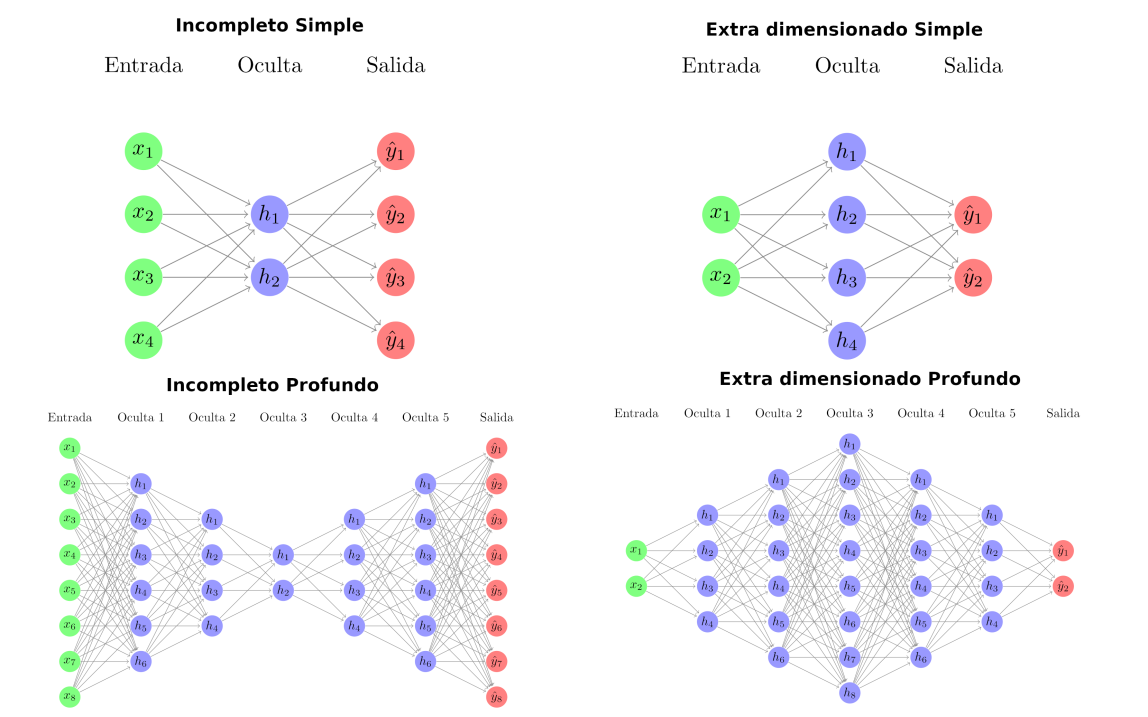
\includegraphics[keepaspectratio]{imagenes/capitulo1/tipos_autoencoders.png}}

}

\caption{\label{fig-tipos_autoencoders}Tipos Arquitectura Autoencoders}

\end{figure}%

Cuando hablamos de \textbf{Incompleto} nos referimos a que tenemos una
reducción de dimensiones que permite llegar a conseguir una
``compresión'' de los datos iniciales como técnica para que aprenda los
patrones internos. En el caso de Extra dimensionado es cuando subimos de
dimensión para conseguir que aprenda esos patrones. En este último caso
sería necesario aplicar técnicas de regularización para evitar que haya
un sobreajuste en el aprendizaje.

Cuando hablamos de \textbf{Simple} estamos haciendo referencia a que hay
una única capa oculta, y en el caso de \textbf{Profundo} es que contamos
con más de una capa oculta.

Normalmente se trabaja con las arquitecturas de tipo Incompleto
profundo, sobre todo cuando se está trabajando con tipos de datos que
son imágenes. Aunque también podríamos encontrar una combinación de
Incompleto con Extra dimensionado profundo cuando trabajamos con tipos
de datos que no son imágenes y así crecer en la primera o segunda capa
oculta, para luego reducir. Esto nos permitiría por ejemplo adaptarnos a
estructuras de AE en las que trabajemos con número de neuronas en una
capa que sean potencia de 2, y poder construir arquitecturas dinámicas
en función del tamaño de los datos, adaptándolos a un tamaño prefijado.

A continuación, vemos un gráfico de una estructura mixta \textbf{Extra
dimensionado - Incompleto profundo.}

\begin{figure}

\centering{

\pandocbounded{\includegraphics[keepaspectratio]{imagenes/capitulo1/autoencoder_mixto.png}}

}

\caption{\label{fig-autoencoder_mixto}Autoencoder Mixto (Incompleto y
Extra dimensionado)}

\end{figure}%

\subsection{Idea intuitiva del uso de
Autoencoders}\label{idea-intuitiva-del-uso-de-autoencoders}

Si un AE trata de reproducir los datos de entrada mediante un encoder y
decoder, \emph{¿que nos puede aportar si ya tenemos los datos de
entrada?}

Ya hemos comentado que la red neuronal de un AE es simétrica y está
formada por un \textbf{encoder} y un \textbf{decoder}, además cuando
trabajamos con los AE que son incompletos, se está produciendo una
\textbf{reducción} del \textbf{tamaño} de los datos en la fase de
codificación y de nuevo una regeneración a partir de esos datos más
pequeños al original. Ya tenemos uno de los conceptos más importantes de
los AE que es la reducción de dimensiones de los datos de entrada. Estas
nuevas variables que se generan una vez pasado el encoder se les suele
llamar el \textbf{espacio latente}.

Este concepto de reducción de dimensiones en el mundo de la minería de
datos lo podemos asimiliar rápidamente a técnicas como el
\textbf{Análisis de Componentes Principales (PCA)}, que nos permite
trabajar con un número más reducido de dimensiones que las originales.
Igualmente, esa reducción de los datos y la capacidad de poder
reconstruir el original podemos asociarlo al concepto de
\textbf{compresión de datos}, de forma que con el encoder podemos
comprimir los datos y con el decoder los podemos descomprimir. En este
caso habría que tener en cuenta que sería una técnica de compresión de
datos con pérdida de información (JPG también es un formato de
compresión con pérdida de compresión). Es decir, con los datos
codificados y el AE (pesos de la red neuronal), seríamos capaces de
volver a regenerar los datos originales.

Otra de las ideas alrededor de los AE es que, si nosotros tenemos un
conjunto de \textbf{datos de la misma naturaleza} y los entrenamos con
nuestro AE, somos capaces de construir una red neuronal (pesos en la red
neuronal) que es capaz de reproducir esos datos a través del AE. Que
ocurre si nosotros metemos un dato que no era de la misma naturaleza que
los que entrenaron el AE, lo que tendremos entonces es que al recrear
los datos originales no va a ser posible que se parezca a los datos de
entrada. De forma que el error que vamos a tener va a ser mucho mayor
por no ser datos de la misma naturaleza. Esto nos puede llevar a
construir un AE que permita detectar anomalías, es decir, que seamos
capaces de detectar cuando un dato es una anomalía porque realmente el
AE no consigue tener un error lo bastante pequeño.

Según lo visto de forma intuitiva vamos a tener el \textbf{encoder}
\(f(X)\) que será el encargado de codificar los datos de entrada y luego
tendremos el \textbf{decoder} \(g(H)\) que será el encargado de realizar
la decodificación y conseguir acercarnos al dato original . Es decir
intentamos conseguir \(g(f(X))=\hat{Y} \approx X\) . Si suponemos un
\textbf{Simple Autoencoder} en el que tenemos una única capa oculta, con
una función de activación intermedia y una función de activación de
salida y los parámetros y represetan los parámetros de la red neuronal
en cada capa, tendríamos la siguiente expresión:

\[
\begin{aligned}
& f(X)=\delta^{(1)}\left(W^{(1)} * X+b^{(1)}\right) \\
& g(H)=\delta^{(2)}\left(W^{(2)} * H+b^{(2)}\right)
\end{aligned}
\]

donde
\(f(g(H))=\delta^{(2)}\left(W^{(2)} *\left(\delta^{(1)}\left(W^{(1)} * H+b^{(1)}\right)+b^{(2)}\right)\right)=\hat{Y} \approx X\)

Así tendremos que \(g(f(X))=\hat{Y}\) donde \(\hat{Y}\) será la
reconstrucción de \(X\).

Una vez tenemos la idea intuitiva de para qué nos puede ayudar un AE,
recopilamos algunos de los \textbf{principales usos} sobre los que
actualmente se está trabajando.

\subsection{Casos de uso}\label{casos-de-uso}

\textbf{Reducción de dimensiones / Compresión de datos}

En la idea intuitiva de los AE ya hemos visto claro que se pueden usar
para la reducción de dimensiones de los datos de entrada. Si estamos
ante unos datos de entrada de tipo estructurado estamos en un caso de
reducción de dimensiones clásico, en el que queremos disminuir el número
de variables con las que trabajar.

Muchas veces este tipo de trabajo se hace mediante el PCA (Análisis de
Componente Principales, por sus siglas en inglés), sabiendo que lo que
se realiza es una transformación lineal de los datos, ya que conseguimos
unas nuevas variables que son una combinación lineal de las mismas. En
el caso de los AE conseguimos mediante las funciones de activación no
lineales (simgmoide, ReLu, tanh, etc) combinaciones no lineales de las
variables originales para reducir las dimensiones. También existen
versiones de PCA no lineales llamadas Kernel PCA que mediante las
técnicas de kernel son capaces de construir relaciones no lineales.

En esta línea estamos viendo que cuando el encoder ha actuado, tenemos
unos nuevos datos más reducidos y que somos capaces de practicamente
volver a reproducir teniendo el decoder. Podríamos pensar en este tipo
de técnica para simplemente comprimir información. Hay que tener en
cuenta que este tipo de técnicas no se pueden aplicar a cualquier dato
que queramos comprimir, ya que debemos haber entrenado al AE con unos
datos de entrenamiento que ha sido capaz de obtener ciertos patrones de
ellos, y por eso es capaz luego de reproducirlos.

\textbf{Búsqueda de imágenes}

Cuando pensamos en un buscador de imágenes nos podemos hacer a la idea
que el buscar al igual que con el texto nos va a mostrar entradas que
seán imágenes parecidas a la que estamos buscando.

Si construimos un autoencoder, el encoder nos va a dar unas variables
con información para poder recrear de nuevo la imagen. Lo que parece
claro es que si hay muy poca distancia entre estas variables y otras la
reconstrucción de la imagen será muy parecida.

Así nosotros podemos entrenar el AE con nuestro conjunto de imágenes,
una vez tenemos el AE pasamos el encoder a todas las imágenes y las
tenemos todas en ese nuevo espacio de variables.

Cuando queremos buscar una imagen, le pasamos el autoencoder, y ya
buscamos las más cercanas a nuestra imagen en el espacio de variables
generado por el encoder.

\textbf{Detección de Anomalías}

Cuando estamos ante un problema de clasificación y tenemos un conjunto
de datos que está muy desbalanceado, es decir, tenemos una clase
mayoritaria que es mucho más grande que la minoritaria (posiblemente del
orden de más del 95\%), muchas veces es complicado conseguir un conjunto
de datos balanceado que sea realmente bueno para hacer las predicciones.

Cuando estamos en estos entornos tan desbalanceados muchas veces se dice
que estamos ante un sistema para detectar \textbf{anomalías}. Un AE nos
puede ayudar a detectar estas anomalías de la siguiente forma:

\begin{itemize}
\tightlist
\item
  Tomamos todos los datos de \textbf{entrenamiento} de la \textbf{clase
  mayoritaria} (o normales) y construimos un AE para ser capaces de
  reproducirlos. Al ser todos estos datos de la misma naturaleza
  conseguiremos entrenar el AE con un error muy pequeño.
\item
  Ahora tomamos los datos de la \textbf{clase} \textbf{minoritaria} (o a
  nomalías) y los pasamos a través del AE obteniendo unos
  \textbf{errores} de \textbf{reconstrucción}.
\item
  Definimos el \textbf{umbral} de error que nos separará los datos
  normales de las anomalías, ya que el AE sólo está entrenado con los
  normales y conseguirá un error más alto con las anomalías al
  reconstruirlas.
\item
  Cogemos los \textbf{datos} de test y los vamos pasando por el AE, si
  el \textbf{error} es \textbf{menor} del \textbf{umbral}, entonces será
  de la \textbf{clase mayoritaria}. Si el error es mayor que el umbral,
  entonces estaremos ante una anomalía.
\end{itemize}

\textbf{Eliminación de ruido}

Otra de las formas de uso de los autoencoders en tratamiento de imágenes
es para eliminar ruido de las mismas, es decir poder quitar manchas de
las imágenes. La forma de hacer esto es la siguiente:

\begin{itemize}
\item
  Partimos de un conjunto de datos de entrenamiento (imágenes) a las que
  le metemos ruido, por ejemplo, modificando los valores de cada pixel
  usando una distribución normal, de forma que obtenemos unos datos de
  entrenamiento con ruido.
\item
  Construimos el AE de forma que los datos de entrada son los que tienen
  ruido, pero los de salida vamos a forzar que sean los originales. De
  forma que intentamos que aprendan a reconstruirse como los que no
  tienen ruido.
\item
  Una vez que tenemos el AE y le pasamos datos de test con ruido,
  seremos capaces de reconstruirlos sin el ruido.
\end{itemize}

\textbf{Modelos generativos}

Cuando hablamos de modelos generativos, nos referimos a AE que son
capaces de generar cosas nuevas a las que existían. De forma que
mediante técnicas como los Variational Autoencoders, los Adversarial
Autoencoders seremos capaces de generar nuevas imágenes que no teníamos
inicialmente. Es decir, podríamos pensar en poder tener un AE que sea
capaz de reconstruir imágenes de caras, pero que además con toda la
información aprendida fuera capaz de generar nuevas caras que realmente
no existen.

\subsection{Diseño del modelo de AE}\label{diseuxf1o-del-modelo-de-ae}

\textbf{Transformación de datos}

Cuando se trabaja con redes neuronales y en particular con AEs,
necesitamos representar los valores de las variables de entrada en forma
numérica. En una red neuronal todos los datos son siempre numéricos.
Esto significa que todas aquellas variables que sean categóricas
necesitamos convertirlas en numéricas. Además es muy conveniente
normalizar los datos para poder trabajar con valores entre 0 y 1, que
van a ayudar a que sea más fácil que se pueda converger a la solución.

Como ya sabemos normalmente nos encontramos que en una red neuronal las
variables de salida son:

\begin{itemize}
\tightlist
\item
  un número (regresión)
\item
  una serie de números (regresión múltiple)
\item
  un dato binario (clasificación binaria)
\item
  un número que representa una categoría (clasifiación múltiple)
\end{itemize}

En el caso de los AE puede que tengamos una gran parte de las veces
valores de series de números, ya que necesitamos volver a representar
los datos de entrada. Esto significa que tendremos que conseguir en la
capa de salida esos datos numéricos que teníamos inicialmente, como si
se tuviera una regresión múltiple.

\textbf{Arquitectura de red}

Como ya se ha comentado en las redes neuronales, algunos de los
hiperparámetros más importantes en un AE son los relacionados con la
arquitectura de la red neuronal.

Para la construcción de un AE vamos a elegir una topología simétrica del
encoder y el decoder.

Durante el diseño del AE necesitaremos ir probando y adaptando todos
estos hiperparámetros de la ANN para conseguir que sea lo más eficiente
posible:

\begin{itemize}
\item
  Número de capas ocultas y neuronas en cada una
\item
  Función de coste y pérdida
\item
  Optimizador
\item
  Función de activación en capas ocultas
\item
  Función de activación en salida
\end{itemize}

\textbf{Número de capas ocultas y neuronas en cada una}

La selección del número de capas ocultas y la cantidad de neuronas en
cada una va a ser un procedimiento de prueba y error en el que se pueden
probar muchas combinaciones. Es cierto que en el caso de trabajar con
imágenes y CNN ya hay muchas arquitecturas definidas y probadas que
consiguen muy buenos resultados. Por otro lado para tipos de datos
estructurados será muy dependiente de esos datos, de forma que será
necesario realizar diferentes pruebas para conseguir un buen resultado.

\textbf{Función de coste y pérdida}

En este caso no hay ninguna recomendación especial para las funciones de
costes/pérdida y dependerá al igual que en las redes neuronales de la
naturaleza de los datos de salida con los que vamos a trabajar.

\textbf{Optimizador}

Se recomienda usar el optimizador \textbf{ADAM} (Diederik P. Kingma
2017) que es el que mejores resultados ha dado en las pruebas según
(Walia 2017), consiguiendo una convergencia más rápida que con el resto
de optimizadores.

\textbf{Función de activación en capas ocultas}

En un AE las funciones de activación en las capas ocultas van a
conseguir establecer las restricciones no lineales al pasar de una capa
a la siguiente, normalmente se evita usar la función de activación
lineal en las capas intermedias ya que queremos conseguir
transformaciones no lineales.

Se recomienda usar la función de activación ReLu en las capas ocultas,
ya que parece ser que es la que mejores resultados da en la convergencia
de la solución y además menor coste computacional tiene a la hora de
realizar los cálculos.

\textbf{Función de activación en salida}

En la capa de salida tenemos que tener en cuenta cual es el tipo de
datos final que queremos obtener, que en el caso de un AE es el mismo
que el tipo de dato de entrada. Normalmente las funciones de activación
que se usarán en la última capa seran:

• Lineal con multiples unidades, para regresión de varios datos
numéricos

• Sigmoid para valores entre 0 y 1

\subsection{Ejemplos de Autoencoders}\label{ejemplos-de-autoencoders}

Una vez entendido el funcionamiento de los AE, veamos algunos de los AE
que se pueden construir para diversas tareas.

\begin{itemize}
\item
  Simple
\item
  Multicapa o Profundo
\item
  Convolucional
\item
  Denoising
\end{itemize}

En la descripción de los tipos de AE vamos a pensar en python y el
framework keras con el backend Tensorflow. Todo el código se proporciona
aparte. Usaremos como \textbf{dataset} a \textbf{MINIST}, que contiene
60.000/10.000 (entrenamiento/validación) \textbf{imágenes} de los
\textbf{números del 0 al 9}, escritos a mano. Cada imagen tiene un
tamaño de 28x28 = 784 pixels, en \textbf{escala de grises}, con lo que
para cada pixel tendremos un valor entre \textbf{0 y 255} para definir
cuál es su intensidad de gris.

\textbf{Autoencoder Simple}

Vamos a describir como construir un \textbf{Autoencoder Simple} usando
una \textbf{red neuronal densamente conectada} en lugar de usar una red
neuronal convolucional, para que sea más sencillo comprender el ejemplo.

Es decir, vamos a tratar los datos de entrada como si fueran unos datos
numéricos que nos da cualquier variable, que queremos reproducir y no
vamos a utilizar ninguna de las técnicas asociadas a las redes
convolucionales. Hay que recordar que las redes convolucionales permiten
mediante un tratamiento de las imágenes (convolución, pooling, etc)
conseguir mejores resultados que si lo hiciéramos directamente con redes
densamente conectadas.

En este caso tendremos una capa de \textbf{entrada} con \textbf{784
neuronas} (correspondientes a los pixels de cada imagen), una capa
\textbf{intermedia} de \textbf{32 neuronas}, y una capa de salida de
nuevo de las 784 neuronas para poder volver a obtener de nuevo los datos
originales.

\begin{Shaded}
\begin{Highlighting}[numbers=left,,]

\ImportTok{import}\NormalTok{ keras}
\ImportTok{from}\NormalTok{ keras }\ImportTok{import}\NormalTok{ layers}

\CommentTok{\# This is the size of our encoded representations}
\NormalTok{encoding\_dim }\OperatorTok{=} \DecValTok{32}  \CommentTok{\# 32 floats {-}\textgreater{} compression of factor 24.5, assuming the input is 784 floats}

\CommentTok{\# This is our input image}
\NormalTok{input\_img }\OperatorTok{=}\NormalTok{ keras.Input(shape}\OperatorTok{=}\NormalTok{(}\DecValTok{784}\NormalTok{,))}
\CommentTok{\# "encoded" is the encoded representation of the input}
\NormalTok{encoded }\OperatorTok{=}\NormalTok{ layers.Dense(encoding\_dim, activation}\OperatorTok{=}\StringTok{\textquotesingle{}relu\textquotesingle{}}\NormalTok{)(input\_img)}
\CommentTok{\# "decoded" is the lossy reconstruction of the input}
\NormalTok{decoded }\OperatorTok{=}\NormalTok{ layers.Dense(}\DecValTok{784}\NormalTok{, activation}\OperatorTok{=}\StringTok{\textquotesingle{}sigmoid\textquotesingle{}}\NormalTok{)(encoded)}

\CommentTok{\# This model maps an input to its reconstruction}
\NormalTok{autoencoder }\OperatorTok{=}\NormalTok{ keras.Model(input\_img, decoded)}

\CommentTok{\# This model maps an input to its encoded representation}
\NormalTok{encoder }\OperatorTok{=}\NormalTok{ keras.Model(input\_img, encoded)}

\CommentTok{\# This is our encoded (32{-}dimensional) input}
\NormalTok{encoded\_input }\OperatorTok{=}\NormalTok{ keras.Input(shape}\OperatorTok{=}\NormalTok{(encoding\_dim,))}
\CommentTok{\# Retrieve the last layer of the autoencoder model}
\NormalTok{decoder\_layer }\OperatorTok{=}\NormalTok{ autoencoder.layers[}\OperatorTok{{-}}\DecValTok{1}\NormalTok{]}
\CommentTok{\# Create the decoder model}
\NormalTok{decoder }\OperatorTok{=}\NormalTok{ keras.Model(encoded\_input, decoder\_layer(encoded\_input))}

\NormalTok{autoencoder.}\BuiltInTok{compile}\NormalTok{(optimizer}\OperatorTok{=}\StringTok{\textquotesingle{}adam\textquotesingle{}}\NormalTok{, loss}\OperatorTok{=}\StringTok{\textquotesingle{}binary\_crossentropy\textquotesingle{}}\NormalTok{)}

\ImportTok{from}\NormalTok{ keras.datasets }\ImportTok{import}\NormalTok{ mnist}
\ImportTok{import}\NormalTok{ numpy }\ImportTok{as}\NormalTok{ np}
\NormalTok{(x\_train, \_), (x\_test, \_) }\OperatorTok{=}\NormalTok{ mnist.load\_data()}

\NormalTok{x\_train }\OperatorTok{=}\NormalTok{ x\_train.astype(}\StringTok{\textquotesingle{}float32\textquotesingle{}}\NormalTok{) }\OperatorTok{/} \FloatTok{255.}
\NormalTok{x\_test }\OperatorTok{=}\NormalTok{ x\_test.astype(}\StringTok{\textquotesingle{}float32\textquotesingle{}}\NormalTok{) }\OperatorTok{/} \FloatTok{255.}
\NormalTok{x\_train }\OperatorTok{=}\NormalTok{ x\_train.reshape((}\BuiltInTok{len}\NormalTok{(x\_train), np.prod(x\_train.shape[}\DecValTok{1}\NormalTok{:])))}
\NormalTok{x\_test }\OperatorTok{=}\NormalTok{ x\_test.reshape((}\BuiltInTok{len}\NormalTok{(x\_test), np.prod(x\_test.shape[}\DecValTok{1}\NormalTok{:])))}
\BuiltInTok{print}\NormalTok{(x\_train.shape)}
\BuiltInTok{print}\NormalTok{(x\_test.shape)}

\NormalTok{autoencoder.fit(x\_train, x\_train,}
\NormalTok{                epochs}\OperatorTok{=}\DecValTok{5}\NormalTok{,}
\NormalTok{                batch\_size}\OperatorTok{=}\DecValTok{256}\NormalTok{,}
\NormalTok{                shuffle}\OperatorTok{=}\VariableTok{True}\NormalTok{,}
\NormalTok{                validation\_data}\OperatorTok{=}\NormalTok{(x\_test, x\_test))}

\CommentTok{\# Encode and decode some digits}
\CommentTok{\# Note that we take them from the *test* set}
\NormalTok{encoded\_imgs }\OperatorTok{=}\NormalTok{ encoder.predict(x\_test)}
\NormalTok{decoded\_imgs }\OperatorTok{=}\NormalTok{ decoder.predict(encoded\_imgs)}

\CommentTok{\# Use Matplotlib (don\textquotesingle{}t ask)}
\ImportTok{import}\NormalTok{ matplotlib.pyplot }\ImportTok{as}\NormalTok{ plt}

\NormalTok{n }\OperatorTok{=} \DecValTok{10}  \CommentTok{\# How many digits we will display}
\NormalTok{plt.figure(figsize}\OperatorTok{=}\NormalTok{(}\DecValTok{20}\NormalTok{, }\DecValTok{4}\NormalTok{))}
\ControlFlowTok{for}\NormalTok{ i }\KeywordTok{in} \BuiltInTok{range}\NormalTok{(n):}
    \CommentTok{\# Display original}
\NormalTok{    ax }\OperatorTok{=}\NormalTok{ plt.subplot(}\DecValTok{2}\NormalTok{, n, i }\OperatorTok{+} \DecValTok{1}\NormalTok{)}
\NormalTok{    plt.imshow(x\_test[i].reshape(}\DecValTok{28}\NormalTok{, }\DecValTok{28}\NormalTok{))}
\NormalTok{    plt.gray()}
\NormalTok{    ax.get\_xaxis().set\_visible(}\VariableTok{False}\NormalTok{)}
\NormalTok{    ax.get\_yaxis().set\_visible(}\VariableTok{False}\NormalTok{)}

    \CommentTok{\# Display reconstruction}
\NormalTok{    ax }\OperatorTok{=}\NormalTok{ plt.subplot(}\DecValTok{2}\NormalTok{, n, i }\OperatorTok{+} \DecValTok{1} \OperatorTok{+}\NormalTok{ n)}
\NormalTok{    plt.imshow(decoded\_imgs[i].reshape(}\DecValTok{28}\NormalTok{, }\DecValTok{28}\NormalTok{))}
\NormalTok{    plt.gray()}
\NormalTok{    ax.get\_xaxis().set\_visible(}\VariableTok{False}\NormalTok{)}
\NormalTok{    ax.get\_yaxis().set\_visible(}\VariableTok{False}\NormalTok{)}
\NormalTok{plt.show()}
\end{Highlighting}
\end{Shaded}

\textbf{Autoencoder Multicapa o profundo}

Vamos a pasar ahora a una versión del autoencoder donde habilitamos
\textbf{más capas ocultas} y hacemos que el descenso del número de
neuronas sea más gradual hasta llegar a nuestro valor deseado, para
luego volver a reconstruirlo.

En este caso seguimos con redes densamente conectadas y aplicamos varias
capas intermedias reduciendo el número de neuronas en cada una hasta
llegar a la capa donde acaba el encoder para volver a ir creciendo en
las sucesivas capas hasta llegar a la de salida.

\begin{Shaded}
\begin{Highlighting}[numbers=left,,]

\ImportTok{import}\NormalTok{ keras}
\ImportTok{from}\NormalTok{ keras }\ImportTok{import}\NormalTok{ layers}

\CommentTok{\# This is the size of our encoded representations}
\NormalTok{encoding\_dim }\OperatorTok{=} \DecValTok{32}  \CommentTok{\# 32 floats {-}\textgreater{} compression of factor 24.5, assuming the input is 784 floats}

\CommentTok{\# This is our input image}
\NormalTok{input\_img }\OperatorTok{=}\NormalTok{ keras.Input(shape}\OperatorTok{=}\NormalTok{(}\DecValTok{784}\NormalTok{,))}
\NormalTok{encoded }\OperatorTok{=}\NormalTok{ layers.Dense(}\DecValTok{128}\NormalTok{, activation}\OperatorTok{=}\StringTok{\textquotesingle{}relu\textquotesingle{}}\NormalTok{)(input\_img)}
\NormalTok{encoded }\OperatorTok{=}\NormalTok{ layers.Dense(}\DecValTok{64}\NormalTok{, activation}\OperatorTok{=}\StringTok{\textquotesingle{}relu\textquotesingle{}}\NormalTok{)(encoded)}
\NormalTok{encoded }\OperatorTok{=}\NormalTok{ layers.Dense(}\DecValTok{32}\NormalTok{, activation}\OperatorTok{=}\StringTok{\textquotesingle{}relu\textquotesingle{}}\NormalTok{)(encoded)}

\NormalTok{decoded }\OperatorTok{=}\NormalTok{ layers.Dense(}\DecValTok{64}\NormalTok{, activation}\OperatorTok{=}\StringTok{\textquotesingle{}relu\textquotesingle{}}\NormalTok{)(encoded)}
\NormalTok{decoded }\OperatorTok{=}\NormalTok{ layers.Dense(}\DecValTok{128}\NormalTok{, activation}\OperatorTok{=}\StringTok{\textquotesingle{}relu\textquotesingle{}}\NormalTok{)(decoded)}
\NormalTok{decoded }\OperatorTok{=}\NormalTok{ layers.Dense(}\DecValTok{784}\NormalTok{, activation}\OperatorTok{=}\StringTok{\textquotesingle{}sigmoid\textquotesingle{}}\NormalTok{)(decoded)}

\CommentTok{\# This model maps an input to its reconstruction}
\NormalTok{autoencoder }\OperatorTok{=}\NormalTok{ keras.Model(input\_img, decoded)}

\CommentTok{\# This model maps an input to its encoded representation}

\NormalTok{autoencoder.}\BuiltInTok{compile}\NormalTok{(optimizer}\OperatorTok{=}\StringTok{\textquotesingle{}adam\textquotesingle{}}\NormalTok{, loss}\OperatorTok{=}\StringTok{\textquotesingle{}binary\_crossentropy\textquotesingle{}}\NormalTok{)}

\ImportTok{from}\NormalTok{ keras.datasets }\ImportTok{import}\NormalTok{ mnist}
\ImportTok{import}\NormalTok{ numpy }\ImportTok{as}\NormalTok{ np}
\NormalTok{(x\_train, \_), (x\_test, \_) }\OperatorTok{=}\NormalTok{ mnist.load\_data()}

\NormalTok{x\_train }\OperatorTok{=}\NormalTok{ x\_train.astype(}\StringTok{\textquotesingle{}float32\textquotesingle{}}\NormalTok{) }\OperatorTok{/} \FloatTok{255.}
\NormalTok{x\_test }\OperatorTok{=}\NormalTok{ x\_test.astype(}\StringTok{\textquotesingle{}float32\textquotesingle{}}\NormalTok{) }\OperatorTok{/} \FloatTok{255.}
\NormalTok{x\_train }\OperatorTok{=}\NormalTok{ x\_train.reshape((}\BuiltInTok{len}\NormalTok{(x\_train), np.prod(x\_train.shape[}\DecValTok{1}\NormalTok{:])))}
\NormalTok{x\_test }\OperatorTok{=}\NormalTok{ x\_test.reshape((}\BuiltInTok{len}\NormalTok{(x\_test), np.prod(x\_test.shape[}\DecValTok{1}\NormalTok{:])))}
\BuiltInTok{print}\NormalTok{(x\_train.shape)}
\BuiltInTok{print}\NormalTok{(x\_test.shape)}

\NormalTok{autoencoder.fit(x\_train, x\_train,}
\NormalTok{                epochs}\OperatorTok{=}\DecValTok{5}\NormalTok{,}
\NormalTok{                batch\_size}\OperatorTok{=}\DecValTok{256}\NormalTok{,}
\NormalTok{                shuffle}\OperatorTok{=}\VariableTok{True}\NormalTok{,}
\NormalTok{                validation\_data}\OperatorTok{=}\NormalTok{(x\_test, x\_test))}

\CommentTok{\# Encode and decode some digits}
\CommentTok{\# Note that we take them from the *test* set}

\NormalTok{decoded\_imgs }\OperatorTok{=}\NormalTok{ autoencoder.predict(x\_test)}
\BuiltInTok{print}\NormalTok{(decoded\_imgs.shape)}
\CommentTok{\# Use Matplotlib (don\textquotesingle{}t ask)}
\ImportTok{import}\NormalTok{ matplotlib.pyplot }\ImportTok{as}\NormalTok{ plt}

\NormalTok{n }\OperatorTok{=} \DecValTok{10}  \CommentTok{\# How many digits we will display}
\NormalTok{plt.figure(figsize}\OperatorTok{=}\NormalTok{(}\DecValTok{20}\NormalTok{, }\DecValTok{4}\NormalTok{))}
\ControlFlowTok{for}\NormalTok{ i }\KeywordTok{in} \BuiltInTok{range}\NormalTok{(n):}
    \CommentTok{\# Display original}
\NormalTok{    ax }\OperatorTok{=}\NormalTok{ plt.subplot(}\DecValTok{2}\NormalTok{, n, i }\OperatorTok{+} \DecValTok{1}\NormalTok{)}
\NormalTok{    plt.imshow(x\_test[i].reshape(}\DecValTok{28}\NormalTok{, }\DecValTok{28}\NormalTok{))}
\NormalTok{    plt.gray()}
\NormalTok{    ax.get\_xaxis().set\_visible(}\VariableTok{False}\NormalTok{)}
\NormalTok{    ax.get\_yaxis().set\_visible(}\VariableTok{False}\NormalTok{)}

    \CommentTok{\# Display reconstruction}
\NormalTok{    ax }\OperatorTok{=}\NormalTok{ plt.subplot(}\DecValTok{2}\NormalTok{, n, i }\OperatorTok{+} \DecValTok{1} \OperatorTok{+}\NormalTok{ n)}
\NormalTok{    plt.imshow(decoded\_imgs[i].reshape(}\DecValTok{28}\NormalTok{, }\DecValTok{28}\NormalTok{))}
\NormalTok{    plt.gray()}
\NormalTok{    ax.get\_xaxis().set\_visible(}\VariableTok{False}\NormalTok{)}
\NormalTok{    ax.get\_yaxis().set\_visible(}\VariableTok{False}\NormalTok{)}
\NormalTok{plt.show()}
\end{Highlighting}
\end{Shaded}

\textbf{Autoencoder Convolucional}

En nuestro ejemplo al estar trabajando con imágenes podemos pasar a
trabajar con Redes Convolucionales (CNN) de forma que en lugar de usar
las capas densamente conectadas que hemos usado hasta ahora, vamos a
pasar a usar las capacidades de las redes convolucionales.

Al trabajar con redes convolucionales necesitaremos trabajar con capas
de convolución o pooling para llegar a la capa donde acaba el encoder
para volver a ir creciendo aplicando operaciones de convolución y
upsampling (contrario al pooling).

En nuestro ejemplo vamos a tener los siguientes elementos.

\begin{Shaded}
\begin{Highlighting}[numbers=left,,]

\ImportTok{import}\NormalTok{ keras}
\ImportTok{from}\NormalTok{ keras }\ImportTok{import}\NormalTok{ layers}

\NormalTok{input\_img }\OperatorTok{=}\NormalTok{ keras.Input(shape}\OperatorTok{=}\NormalTok{(}\DecValTok{28}\NormalTok{, }\DecValTok{28}\NormalTok{, }\DecValTok{1}\NormalTok{))}

\NormalTok{x }\OperatorTok{=}\NormalTok{ layers.Conv2D(}\DecValTok{16}\NormalTok{, (}\DecValTok{3}\NormalTok{, }\DecValTok{3}\NormalTok{), activation}\OperatorTok{=}\StringTok{\textquotesingle{}relu\textquotesingle{}}\NormalTok{, padding}\OperatorTok{=}\StringTok{\textquotesingle{}same\textquotesingle{}}\NormalTok{)(input\_img)}
\NormalTok{x }\OperatorTok{=}\NormalTok{ layers.MaxPooling2D((}\DecValTok{2}\NormalTok{, }\DecValTok{2}\NormalTok{), padding}\OperatorTok{=}\StringTok{\textquotesingle{}same\textquotesingle{}}\NormalTok{)(x)}
\NormalTok{x }\OperatorTok{=}\NormalTok{ layers.Conv2D(}\DecValTok{8}\NormalTok{, (}\DecValTok{3}\NormalTok{, }\DecValTok{3}\NormalTok{), activation}\OperatorTok{=}\StringTok{\textquotesingle{}relu\textquotesingle{}}\NormalTok{, padding}\OperatorTok{=}\StringTok{\textquotesingle{}same\textquotesingle{}}\NormalTok{)(x)}
\NormalTok{x }\OperatorTok{=}\NormalTok{ layers.MaxPooling2D((}\DecValTok{2}\NormalTok{, }\DecValTok{2}\NormalTok{), padding}\OperatorTok{=}\StringTok{\textquotesingle{}same\textquotesingle{}}\NormalTok{)(x)}
\NormalTok{x }\OperatorTok{=}\NormalTok{ layers.Conv2D(}\DecValTok{8}\NormalTok{, (}\DecValTok{3}\NormalTok{, }\DecValTok{3}\NormalTok{), activation}\OperatorTok{=}\StringTok{\textquotesingle{}relu\textquotesingle{}}\NormalTok{, padding}\OperatorTok{=}\StringTok{\textquotesingle{}same\textquotesingle{}}\NormalTok{)(x)}
\NormalTok{encoded }\OperatorTok{=}\NormalTok{ layers.MaxPooling2D((}\DecValTok{2}\NormalTok{, }\DecValTok{2}\NormalTok{), padding}\OperatorTok{=}\StringTok{\textquotesingle{}same\textquotesingle{}}\NormalTok{)(x)}

\CommentTok{\# at this point the representation is (4, 4, 8) i.e. 128{-}dimensional}

\NormalTok{x }\OperatorTok{=}\NormalTok{ layers.Conv2D(}\DecValTok{8}\NormalTok{, (}\DecValTok{3}\NormalTok{, }\DecValTok{3}\NormalTok{), activation}\OperatorTok{=}\StringTok{\textquotesingle{}relu\textquotesingle{}}\NormalTok{, padding}\OperatorTok{=}\StringTok{\textquotesingle{}same\textquotesingle{}}\NormalTok{)(encoded)}
\NormalTok{x }\OperatorTok{=}\NormalTok{ layers.UpSampling2D((}\DecValTok{2}\NormalTok{, }\DecValTok{2}\NormalTok{))(x)}
\NormalTok{x }\OperatorTok{=}\NormalTok{ layers.Conv2D(}\DecValTok{8}\NormalTok{, (}\DecValTok{3}\NormalTok{, }\DecValTok{3}\NormalTok{), activation}\OperatorTok{=}\StringTok{\textquotesingle{}relu\textquotesingle{}}\NormalTok{, padding}\OperatorTok{=}\StringTok{\textquotesingle{}same\textquotesingle{}}\NormalTok{)(x)}
\NormalTok{x }\OperatorTok{=}\NormalTok{ layers.UpSampling2D((}\DecValTok{2}\NormalTok{, }\DecValTok{2}\NormalTok{))(x)}
\NormalTok{x }\OperatorTok{=}\NormalTok{ layers.Conv2D(}\DecValTok{16}\NormalTok{, (}\DecValTok{3}\NormalTok{, }\DecValTok{3}\NormalTok{), activation}\OperatorTok{=}\StringTok{\textquotesingle{}relu\textquotesingle{}}\NormalTok{)(x)}
\NormalTok{x }\OperatorTok{=}\NormalTok{ layers.UpSampling2D((}\DecValTok{2}\NormalTok{, }\DecValTok{2}\NormalTok{))(x)}
\NormalTok{decoded }\OperatorTok{=}\NormalTok{ layers.Conv2D(}\DecValTok{1}\NormalTok{, (}\DecValTok{3}\NormalTok{, }\DecValTok{3}\NormalTok{), activation}\OperatorTok{=}\StringTok{\textquotesingle{}sigmoid\textquotesingle{}}\NormalTok{, padding}\OperatorTok{=}\StringTok{\textquotesingle{}same\textquotesingle{}}\NormalTok{)(x)}

\NormalTok{autoencoder }\OperatorTok{=}\NormalTok{ keras.Model(input\_img, decoded)}
\NormalTok{autoencoder.}\BuiltInTok{compile}\NormalTok{(optimizer}\OperatorTok{=}\StringTok{\textquotesingle{}adam\textquotesingle{}}\NormalTok{, loss}\OperatorTok{=}\StringTok{\textquotesingle{}binary\_crossentropy\textquotesingle{}}\NormalTok{)}

\ImportTok{from}\NormalTok{ keras.datasets }\ImportTok{import}\NormalTok{ mnist}
\ImportTok{import}\NormalTok{ numpy }\ImportTok{as}\NormalTok{ np}

\NormalTok{(x\_train, \_), (x\_test, \_) }\OperatorTok{=}\NormalTok{ mnist.load\_data()}

\NormalTok{x\_train }\OperatorTok{=}\NormalTok{ x\_train.astype(}\StringTok{\textquotesingle{}float32\textquotesingle{}}\NormalTok{) }\OperatorTok{/} \FloatTok{255.}
\NormalTok{x\_test }\OperatorTok{=}\NormalTok{ x\_test.astype(}\StringTok{\textquotesingle{}float32\textquotesingle{}}\NormalTok{) }\OperatorTok{/} \FloatTok{255.}
\NormalTok{x\_train }\OperatorTok{=}\NormalTok{ np.reshape(x\_train, (}\BuiltInTok{len}\NormalTok{(x\_train), }\DecValTok{28}\NormalTok{, }\DecValTok{28}\NormalTok{, }\DecValTok{1}\NormalTok{))}
\NormalTok{x\_test }\OperatorTok{=}\NormalTok{ np.reshape(x\_test, (}\BuiltInTok{len}\NormalTok{(x\_test), }\DecValTok{28}\NormalTok{, }\DecValTok{28}\NormalTok{, }\DecValTok{1}\NormalTok{))}


\NormalTok{autoencoder.fit(x\_train, x\_train,}
\NormalTok{                epochs}\OperatorTok{=}\DecValTok{5}\NormalTok{,}
\NormalTok{                batch\_size}\OperatorTok{=}\DecValTok{128}\NormalTok{,}
\NormalTok{                shuffle}\OperatorTok{=}\VariableTok{True}\NormalTok{,}
\NormalTok{                validation\_data}\OperatorTok{=}\NormalTok{(x\_test, x\_test))}

\NormalTok{decoded\_imgs }\OperatorTok{=}\NormalTok{ autoencoder.predict(x\_test)}

\NormalTok{n }\OperatorTok{=} \DecValTok{10}
\NormalTok{plt.figure(figsize}\OperatorTok{=}\NormalTok{(}\DecValTok{20}\NormalTok{, }\DecValTok{4}\NormalTok{))}
\ControlFlowTok{for}\NormalTok{ i }\KeywordTok{in} \BuiltInTok{range}\NormalTok{(}\DecValTok{1}\NormalTok{, n }\OperatorTok{+} \DecValTok{1}\NormalTok{):}
    \CommentTok{\# Display original}
\NormalTok{    ax }\OperatorTok{=}\NormalTok{ plt.subplot(}\DecValTok{2}\NormalTok{, n, i)}
\NormalTok{    plt.imshow(x\_test[i].reshape(}\DecValTok{28}\NormalTok{, }\DecValTok{28}\NormalTok{))}
\NormalTok{    plt.gray()}
\NormalTok{    ax.get\_xaxis().set\_visible(}\VariableTok{False}\NormalTok{)}
\NormalTok{    ax.get\_yaxis().set\_visible(}\VariableTok{False}\NormalTok{)}

    \CommentTok{\# Display reconstruction}
\NormalTok{    ax }\OperatorTok{=}\NormalTok{ plt.subplot(}\DecValTok{2}\NormalTok{, n, i }\OperatorTok{+}\NormalTok{ n)}
\NormalTok{    plt.imshow(decoded\_imgs[i].reshape(}\DecValTok{28}\NormalTok{, }\DecValTok{28}\NormalTok{))}
\NormalTok{    plt.gray()}
\NormalTok{    ax.get\_xaxis().set\_visible(}\VariableTok{False}\NormalTok{)}
\NormalTok{    ax.get\_yaxis().set\_visible(}\VariableTok{False}\NormalTok{)}
\NormalTok{plt.show()}
\end{Highlighting}
\end{Shaded}

\textbf{Autoencoder Denoising}

Vaamos a usar ahora un autoencoder para hacer limpieza en imagen, es
decir, conseguir a partir de una imagen que tiene ruido otra imagen sin
ese ruido. Entrenaremos al autoencoder para que limpie ``ruido'' que hay
en la imagen y lo reconstruya sin ello. El ruido lo vamos a generar
mediante una distribución normal y modificaremos el valor de los pixels
de las imágenes.

Usaremos estas imágenes con ruido para que sea capaz de reconstruir la
imagen original sin ruido con el AE. Para realizar este proceso lo que
haremos será:

• Crear nuevas imágenes con ruido

• Entrenar el autoencoder con estas nuevas imágenes

• Calcular el error de reconstrucción respecto a las imágenes originales

Al estar trabajando con imágenes vamos a partir del Autoencoder de
Convolución para poder aplicar el denosing.

\begin{Shaded}
\begin{Highlighting}[numbers=left,,]
\ImportTok{import}\NormalTok{ keras}
\ImportTok{from}\NormalTok{ keras }\ImportTok{import}\NormalTok{ layers}

\NormalTok{input\_img }\OperatorTok{=}\NormalTok{ keras.Input(shape}\OperatorTok{=}\NormalTok{(}\DecValTok{28}\NormalTok{, }\DecValTok{28}\NormalTok{, }\DecValTok{1}\NormalTok{))}

\NormalTok{x }\OperatorTok{=}\NormalTok{ layers.Conv2D(}\DecValTok{16}\NormalTok{, (}\DecValTok{3}\NormalTok{, }\DecValTok{3}\NormalTok{), activation}\OperatorTok{=}\StringTok{\textquotesingle{}relu\textquotesingle{}}\NormalTok{, padding}\OperatorTok{=}\StringTok{\textquotesingle{}same\textquotesingle{}}\NormalTok{)(input\_img)}
\NormalTok{x }\OperatorTok{=}\NormalTok{ layers.MaxPooling2D((}\DecValTok{2}\NormalTok{, }\DecValTok{2}\NormalTok{), padding}\OperatorTok{=}\StringTok{\textquotesingle{}same\textquotesingle{}}\NormalTok{)(x)}
\NormalTok{x }\OperatorTok{=}\NormalTok{ layers.Conv2D(}\DecValTok{8}\NormalTok{, (}\DecValTok{3}\NormalTok{, }\DecValTok{3}\NormalTok{), activation}\OperatorTok{=}\StringTok{\textquotesingle{}relu\textquotesingle{}}\NormalTok{, padding}\OperatorTok{=}\StringTok{\textquotesingle{}same\textquotesingle{}}\NormalTok{)(x)}
\NormalTok{x }\OperatorTok{=}\NormalTok{ layers.MaxPooling2D((}\DecValTok{2}\NormalTok{, }\DecValTok{2}\NormalTok{), padding}\OperatorTok{=}\StringTok{\textquotesingle{}same\textquotesingle{}}\NormalTok{)(x)}
\NormalTok{x }\OperatorTok{=}\NormalTok{ layers.Conv2D(}\DecValTok{8}\NormalTok{, (}\DecValTok{3}\NormalTok{, }\DecValTok{3}\NormalTok{), activation}\OperatorTok{=}\StringTok{\textquotesingle{}relu\textquotesingle{}}\NormalTok{, padding}\OperatorTok{=}\StringTok{\textquotesingle{}same\textquotesingle{}}\NormalTok{)(x)}
\NormalTok{encoded }\OperatorTok{=}\NormalTok{ layers.MaxPooling2D((}\DecValTok{2}\NormalTok{, }\DecValTok{2}\NormalTok{), padding}\OperatorTok{=}\StringTok{\textquotesingle{}same\textquotesingle{}}\NormalTok{)(x)}

\CommentTok{\# at this point the representation is (4, 4, 8) i.e. 128{-}dimensional}

\NormalTok{x }\OperatorTok{=}\NormalTok{ layers.Conv2D(}\DecValTok{8}\NormalTok{, (}\DecValTok{3}\NormalTok{, }\DecValTok{3}\NormalTok{), activation}\OperatorTok{=}\StringTok{\textquotesingle{}relu\textquotesingle{}}\NormalTok{, padding}\OperatorTok{=}\StringTok{\textquotesingle{}same\textquotesingle{}}\NormalTok{)(encoded)}
\NormalTok{x }\OperatorTok{=}\NormalTok{ layers.UpSampling2D((}\DecValTok{2}\NormalTok{, }\DecValTok{2}\NormalTok{))(x)}
\NormalTok{x }\OperatorTok{=}\NormalTok{ layers.Conv2D(}\DecValTok{8}\NormalTok{, (}\DecValTok{3}\NormalTok{, }\DecValTok{3}\NormalTok{), activation}\OperatorTok{=}\StringTok{\textquotesingle{}relu\textquotesingle{}}\NormalTok{, padding}\OperatorTok{=}\StringTok{\textquotesingle{}same\textquotesingle{}}\NormalTok{)(x)}
\NormalTok{x }\OperatorTok{=}\NormalTok{ layers.UpSampling2D((}\DecValTok{2}\NormalTok{, }\DecValTok{2}\NormalTok{))(x)}
\NormalTok{x }\OperatorTok{=}\NormalTok{ layers.Conv2D(}\DecValTok{16}\NormalTok{, (}\DecValTok{3}\NormalTok{, }\DecValTok{3}\NormalTok{), activation}\OperatorTok{=}\StringTok{\textquotesingle{}relu\textquotesingle{}}\NormalTok{)(x)}
\NormalTok{x }\OperatorTok{=}\NormalTok{ layers.UpSampling2D((}\DecValTok{2}\NormalTok{, }\DecValTok{2}\NormalTok{))(x)}
\NormalTok{decoded }\OperatorTok{=}\NormalTok{ layers.Conv2D(}\DecValTok{1}\NormalTok{, (}\DecValTok{3}\NormalTok{, }\DecValTok{3}\NormalTok{), activation}\OperatorTok{=}\StringTok{\textquotesingle{}sigmoid\textquotesingle{}}\NormalTok{, padding}\OperatorTok{=}\StringTok{\textquotesingle{}same\textquotesingle{}}\NormalTok{)(x)}

\NormalTok{autoencoder }\OperatorTok{=}\NormalTok{ keras.Model(input\_img, decoded)}
\NormalTok{autoencoder.}\BuiltInTok{compile}\NormalTok{(optimizer}\OperatorTok{=}\StringTok{\textquotesingle{}adam\textquotesingle{}}\NormalTok{, loss}\OperatorTok{=}\StringTok{\textquotesingle{}binary\_crossentropy\textquotesingle{}}\NormalTok{)}

\ImportTok{from}\NormalTok{ keras.datasets }\ImportTok{import}\NormalTok{ mnist}
\ImportTok{import}\NormalTok{ numpy }\ImportTok{as}\NormalTok{ np}

\NormalTok{(x\_train, \_), (x\_test, \_) }\OperatorTok{=}\NormalTok{ mnist.load\_data()}

\NormalTok{x\_train }\OperatorTok{=}\NormalTok{ x\_train.astype(}\StringTok{\textquotesingle{}float32\textquotesingle{}}\NormalTok{) }\OperatorTok{/} \FloatTok{255.}
\NormalTok{x\_test }\OperatorTok{=}\NormalTok{ x\_test.astype(}\StringTok{\textquotesingle{}float32\textquotesingle{}}\NormalTok{) }\OperatorTok{/} \FloatTok{255.}
\NormalTok{x\_train }\OperatorTok{=}\NormalTok{ np.reshape(x\_train, (}\BuiltInTok{len}\NormalTok{(x\_train), }\DecValTok{28}\NormalTok{, }\DecValTok{28}\NormalTok{, }\DecValTok{1}\NormalTok{))}
\NormalTok{x\_test }\OperatorTok{=}\NormalTok{ np.reshape(x\_test, (}\BuiltInTok{len}\NormalTok{(x\_test), }\DecValTok{28}\NormalTok{, }\DecValTok{28}\NormalTok{, }\DecValTok{1}\NormalTok{))}

\NormalTok{noise\_factor }\OperatorTok{=} \FloatTok{0.5}
\NormalTok{x\_train\_noisy }\OperatorTok{=}\NormalTok{ x\_train }\OperatorTok{+}\NormalTok{ noise\_factor }\OperatorTok{*}\NormalTok{ np.random.normal(loc}\OperatorTok{=}\FloatTok{0.0}\NormalTok{, scale}\OperatorTok{=}\FloatTok{1.0}\NormalTok{, size}\OperatorTok{=}\NormalTok{x\_train.shape) }
\NormalTok{x\_test\_noisy }\OperatorTok{=}\NormalTok{ x\_test }\OperatorTok{+}\NormalTok{ noise\_factor }\OperatorTok{*}\NormalTok{ np.random.normal(loc}\OperatorTok{=}\FloatTok{0.0}\NormalTok{, scale}\OperatorTok{=}\FloatTok{1.0}\NormalTok{, size}\OperatorTok{=}\NormalTok{x\_test.shape) }

\NormalTok{x\_train\_noisy }\OperatorTok{=}\NormalTok{ np.clip(x\_train\_noisy, }\FloatTok{0.}\NormalTok{, }\FloatTok{1.}\NormalTok{)}
\NormalTok{x\_test\_noisy }\OperatorTok{=}\NormalTok{ np.clip(x\_test\_noisy, }\FloatTok{0.}\NormalTok{, }\FloatTok{1.}\NormalTok{)}


\NormalTok{n }\OperatorTok{=} \DecValTok{10}
\NormalTok{plt.figure(figsize}\OperatorTok{=}\NormalTok{(}\DecValTok{20}\NormalTok{, }\DecValTok{2}\NormalTok{))}
\ControlFlowTok{for}\NormalTok{ i }\KeywordTok{in} \BuiltInTok{range}\NormalTok{(}\DecValTok{1}\NormalTok{, n }\OperatorTok{+} \DecValTok{1}\NormalTok{):}
\NormalTok{    ax }\OperatorTok{=}\NormalTok{ plt.subplot(}\DecValTok{1}\NormalTok{, n, i)}
\NormalTok{    plt.imshow(x\_test\_noisy[i].reshape(}\DecValTok{28}\NormalTok{, }\DecValTok{28}\NormalTok{))}
\NormalTok{    plt.gray()}
\NormalTok{    ax.get\_xaxis().set\_visible(}\VariableTok{False}\NormalTok{)}
\NormalTok{    ax.get\_yaxis().set\_visible(}\VariableTok{False}\NormalTok{)}
\NormalTok{plt.show()}


\NormalTok{autoencoder.fit(x\_train\_noisy, x\_train,}
\NormalTok{                epochs}\OperatorTok{=}\DecValTok{5}\NormalTok{,}
\NormalTok{                batch\_size}\OperatorTok{=}\DecValTok{128}\NormalTok{,}
\NormalTok{                shuffle}\OperatorTok{=}\VariableTok{True}\NormalTok{,}
\NormalTok{                validation\_data}\OperatorTok{=}\NormalTok{(x\_test\_noisy, x\_test))}


\NormalTok{decoded\_imgs }\OperatorTok{=}\NormalTok{ autoencoder.predict(x\_test)}

\NormalTok{n }\OperatorTok{=} \DecValTok{10}
\NormalTok{plt.figure(figsize}\OperatorTok{=}\NormalTok{(}\DecValTok{20}\NormalTok{, }\DecValTok{4}\NormalTok{))}
\ControlFlowTok{for}\NormalTok{ i }\KeywordTok{in} \BuiltInTok{range}\NormalTok{(}\DecValTok{1}\NormalTok{, n }\OperatorTok{+} \DecValTok{1}\NormalTok{):}
    \CommentTok{\# Display original}
\NormalTok{    ax }\OperatorTok{=}\NormalTok{ plt.subplot(}\DecValTok{2}\NormalTok{, n, i)}
\NormalTok{    plt.imshow(x\_test\_noisy[i].reshape(}\DecValTok{28}\NormalTok{, }\DecValTok{28}\NormalTok{))}
\NormalTok{    plt.gray()}
\NormalTok{    ax.get\_xaxis().set\_visible(}\VariableTok{False}\NormalTok{)}
\NormalTok{    ax.get\_yaxis().set\_visible(}\VariableTok{False}\NormalTok{)}

    \CommentTok{\# Display reconstruction}
\NormalTok{    ax }\OperatorTok{=}\NormalTok{ plt.subplot(}\DecValTok{2}\NormalTok{, n, i }\OperatorTok{+}\NormalTok{ n)}
\NormalTok{    plt.imshow(decoded\_imgs[i].reshape(}\DecValTok{28}\NormalTok{, }\DecValTok{28}\NormalTok{))}
\NormalTok{    plt.gray()}
\NormalTok{    ax.get\_xaxis().set\_visible(}\VariableTok{False}\NormalTok{)}
\NormalTok{    ax.get\_yaxis().set\_visible(}\VariableTok{False}\NormalTok{)}
\NormalTok{plt.show()}
\end{Highlighting}
\end{Shaded}

\section{Arquitecturas preentrenadas}\label{arquitecturas-preentrenadas}

Las \textbf{arquitecturas pre-entrenadas} en Deep Learning son modelos
de redes neuronales que han sido previamente entrenados en grandes
conjuntos de datos para realizar tareas específicas como clasificación
de imágenes, generación de texto o reconocimiento de voz. Durante el
entrenamiento, estos modelos aprenden patrones complejos de los datos,
lo que les permite realizar tareas relacionadas con alta precisión y
generalización.

El funcionamiento de las arquitecturas pre-entrenadas se basa en el
concepto de \textbf{transferencia de aprendizaje}. La transferencia de
aprendizaje consiste en aprovechar el conocimiento aprendido en una
tarea para aplicarlo a otra tarea diferente; es decir, se utiliza como
base para realizar tareas específicas con mayor facilidad.

Las arquitecturas pre-entrenadas suelen ser diseñadas por investigadores
y equipos de desarrollo en instituciones académicas, laboratorios de
investigación y empresas de tecnología. Estos expertos desarrollan las
arquitecturas, definen el proceso de entrenamiento y seleccionan los
conjuntos de datos adecuados para cada tarea. Algunas de las
organizaciones e instituciones que lideran el diseño de arquitecturas
pre-entrenadas son:

\begin{itemize}
\tightlist
\item
  \emph{Google AI}: ha desarrollado arquitecturas pre-entrenadas como
  BERT y Vision Transformers, las cuales han tenido un gran impacto en
  el procesamiento del lenguaje natural y la visión artificial,
  respectivamente. Además, en los últimos años, han publicado Gema y
  Gemini, que permiten el aprendizaje automático en general, ofreciendo
  flexibilidad, escalabilidad y alto rendimiento en diversas tareas
\item
  \emph{Facebook AI Research}: ha contribuido con arquitecturas
  pre-entrenadas como FAIRSEQ y Detectron2, que han impulsado el
  rendimiento en tareas de procesamiento del lenguaje natural y
  detección de objetos, respectivamente. Además, también ha desarrollado
  Llama, Llama2 y Llama3, modelos que han destacado por su versatilidad
  y precisión en aplicaciones de reconocimiento de voz y procesamiento
  de texto.
\item
  \emph{OpenAI}: conocido por sus arquitecturas pre-entrenadas líderes
  como GPT-3 y Whisper, ha lanzado recientemente GPT-4. Este modelo
  promete mejorar la comprensión contextual y la generación de texto, lo
  que podría tener un gran impacto en aplicaciones de procesamiento del
  lenguaje natural. GPT-4 representa un avance significativo en la
  investigación de inteligencia artificial y abre nuevas posibilidades
  para sistemas más avanzados.
\end{itemize}

Estos modelos son entrenados en grandes clústeres de servidores con
hardware especializado, como GPUs y TPUs, utilizando conjuntos de datos
masivos y técnicas de optimización avanzadas. A día de hoy se han
convertido en un elemento capital para los desarrolladores de
aprendizaje automático puesto que nos permite aprovechar modelos
entrenados previamente que, en condiciones normales, sería casi
imposible realizar por centros no especializados. Así, podríamos
destacar las siguientes ventajas:

\begin{itemize}
\tightlist
\item
  Ahorro de tiempo y recursos: al aprovechar el conocimiento
  pre-entrenado, nos permiten a los desarrolladores ahorrar tiempo y
  recursos computacionales en comparación con entrenar un modelo desde
  cero
\item
  Mayor rendimiento: suelen ofrecer un rendimiento superior a los
  modelos entrenados desde cero, especialmente para tareas complejas
\item
  Facilidad de uso: las librerías y entornos facilitan el acceso y la
  utilización de arquitecturas pre-entrenadas, incluso para usuarios con
  poca experiencia en Deep Learning
\end{itemize}

Como se ha dicho, cada vez más se emplean este tipo de arquitecturas
para realizar tareas que, con otro tipo de diseños de aprendizaje
automático serían más complejas y costosas de abordar. En este aspecto,
destacar que a la hora de elegir qué tipo de arquitectura pre-entrenada
es adecuada para un caso de uso es necesario tener en cuenta la tarea
específica a abordar, el conjunto de datos con los que ha sido entrenada
y la similaridad con los nuestros propios así como si disponemos de
ciertas limitaciones en cuanto a recursos computacionales.

Por último, destacar que existen diversas librerías y entornos que
facilitan el trabajo con arquitecturas pre-entrenadas. Algunas de las
opciones más interesantes son:

- TensorFlow Hub: es un repositorio de módulos pre-entrenados para
TensorFlow, que incluye una amplia gama de arquitecturas pre-entrenadas
para diversas tareas. - Hugging Face Hub: es una plataforma similar a
TensorFlow Hub, pero que ofrece soporte para múltiples frameworks de
Deep Learning, incluyendo TensorFlow, PyTorch y JAX.

\subsection{Paquetes específicos en
Python}\label{paquetes-especuxedficos-en-python}

\subsubsection{Transformers}\label{transformers}

Transformers es una biblioteca de código abierto en Python desarrollada
por Hugging Face que proporciona un conjunto de herramientas para
trabajar con modelos de lenguaje basados en redes neuronales
transformadoras.

Esta librería se caracteriza por su gran variedad de modelos
pre-entrenados y capacidad de hacer fine-tuning de modelos. Así, entre
sus principales ventajas podemos citar: - La facilidad de uso - La
flexibilidad y la escalabilidad - La comunidad activa de desarrolladores

Finalmente, indicamos proporcionamos una serie de recursos adicionales:

\begin{itemize}
\tightlist
\item
  Sitio web de Transformers:
  \url{https://huggingface.co/docs/transformers/en/index}
\item
  Documentación de Transformers: \url{https://huggingface.co/docs}
\item
  Tutoriales de Transformers:
  \url{https://www.youtube.com/watch?v=QEaBAZQCtwE}
\end{itemize}

\subsection{Tensorflow-Hub}\label{tensorflow-hub}

Tensorflow-Hub alberga una gran colección de módulos de aprendizaje
automático pre-entrenados y reutilizables, creados por Google y la
comunidad de TensorFlow.

Esta librería se caracteriza por disponer de una gran cantidad de
modelos pre-entrenados para diferentes tareas relacionadas con el
aprendizaje profundo. Así, entre sus principales ventajas podemos citar:
- El acceso a modelos pre-entrenados de última generación - La
flexibilidad y personalización - La facilidad de

Finalmente, indicamos proporcionamos una serie de recursos adicionales:

\begin{itemize}
\tightlist
\item
  Sitio web de TensorFlow Hub: \url{https://www.tensorflow.org/hub}
\item
  Documentación de TensorFlow Hub: \url{https://www.tensorflow.org/hub}
\item
  Tutoriales de TensorFlow Hub:
  \url{https://www.tensorflow.org/hub/tutorials}
\end{itemize}

\subsection{Arquitecturas Zero-shot}\label{arquitecturas-zero-shot}

Las \textbf{arquitecturas Zero-Shot}, también conocidas como
\emph{modelos de Aprendizaje por Analogía} son capaces de realizar
tareas de clasificación sin necesidad de entrenamiento específico para
cada categoría. En su lugar, estas arquitecturas aprenden
representaciones vectoriales de conceptos a partir de datos no
etiquetados, lo que les permite generalizar a nuevas categorías sin
haberlas visto nunca antes.

\begin{figure}

\centering{

\pandocbounded{\includegraphics[keepaspectratio]{imagenes/capitulo1/zero-shot.png}}

}

\caption{\label{fig-redneuronal}Red Neuronal Clasica}

\end{figure}%

\subsubsection{Uso en imágenes}\label{uso-en-imuxe1genes}

En el ámbito de la visión artificial, las arquitecturas Zero-Shot para
imágenes han demostrado ser particularmente útiles para tareas como la
clasificación de imágenes de escenas naturales, la identificación de
animales y la detección de objetos. Entre los modelos más destacados en
esta área se encuentran: - \emph{ImageNet-pretrained CLIP}: basado en la
arquitectura CLIP (Contrastive Language-Image Pre-training), este modelo
utiliza representaciones de imágenes y texto para realizar clasificación
Zero-Shot de imágenes con gran precisión - \emph{ResNet-pretrained ZSL}:
Este modelo combina la arquitectura ResNet, conocida por su rendimiento
en tareas de clasificación de imágenes, con un enfoque Zero-Shot basado
en la distancia entre representaciones

\texttt{MATERIAL\ COMPLEMENTARIO\ -\ NOTEBOOK}: ejemplo en
\texttt{Zero-shot:\ clasificación\ animales}

\subsubsection{Uso en texto}\label{uso-en-texto}

En el procesamiento del lenguaje natural, las arquitecturas Zero-Shot
para texto han ganado popularidad para tareas como la clasificación de
documentos, la extracción de información y la categorización de textos.
Algunos modelos representativos en este campo son:

\begin{itemize}
\tightlist
\item
  \emph{BERT-pretrained ZSL}: basado en la arquitectura BERT
  (Bidirectional Encoder Representations from Transformers), este modelo
  utiliza representaciones contextuales de palabras para realizar
  clasificación Zero-Shot de texto con gran precisión
\item
  \emph{Siamese Networks with Word Embeddings}: este enfoque utiliza
  redes siamesas, un tipo de red neuronal que aprende a comparar pares
  de entradas, para clasificar texto Zero-Shot utilizando
  representaciones de palabras pre-entrenadas.
\end{itemize}

\subsection{Detección de objetos}\label{detecciuxf3n-de-objetos}

La \textbf{detección de objetos} es una tarea fundamental en el ámbito
de la visión artificial, que consiste en identificar y localizar objetos
dentro de una imagen o video. Las arquitecturas pre-entrenadas para la
detección de objetos han revolucionado este campo, ofreciendo modelos de
alta precisión y eficiencia. Entre los modelos más utilizados se
encuentran:

\begin{itemize}
\tightlist
\item
  \emph{Faster R-CNN}: Este modelo combina la arquitectura de redes
  convolucionales profundas (CNN) con una región de propuesta de
  regiones (RPN) para detectar y localizar objetos con gran precisión
\item
  \emph{YOLOv5}: Este modelo destaca por su velocidad y eficiencia,
  utilizando una arquitectura basada en convoluciones y bloques de
  atención para detectar objetos en tiempo real
\end{itemize}

\texttt{MATERIAL\ COMPLEMENTARIO\ -\ VIDEOTUTORIAL}: ejemplo en
\texttt{Arquitecturas\ Tensorflow-Hub}

\subsection{Conversión de voz a
texto}\label{conversiuxf3n-de-voz-a-texto}

La \emph{conversión de voz a texto}, también llamado como
\textbf{Speech-to-Text} es una tarea crucial para la interacción
hombre-máquina. Las arquitecturas pre-entrenadas para este tipo de casos
han impulsado el desarrollo de sistemas de reconocimiento de voz de alta
precisión, capaces de transcribir audio en texto con gran fluidez. Uno
de los principales modelos para esta tarea es \emph{Whisper} el cual fue
desarrollado por OpenAI. Este modelo se basa en la arquitectura
\emph{Transformer} y utiliza aprendizaje supervisado y multitarea para
lograr una precisión y robustez excepcionales en una amplia gama de
condiciones acústicas.

\texttt{MATERIAL\ COMPLEMENTARIO\ -\ VIDEOTUTORIAL}: ejemplo en
\texttt{Speech2Text}

\section{Aprendizaje por Refuerzo}\label{aprendizaje-por-refuerzo}

\subsection{Introducción}\label{introducciuxf3n-2}

Hasta ahora hemos visto como el Deep Learning se usa para el
\textbf{aprendizaje supervisado} y el \textbf{aprendizaje no
supervisado}, pero vamos a dar un paso más, en el que veremos como usar
Deep Learning en otro tipo de aprendizaje llamado \textbf{aprendizaje
por refuerzo}.

El \textbf{Aprendizaje por Refuerzo} (\textbf{RL} por sus siglas en
ingles, \textbf{Reinforcement Learning}) trata de conseguir que el
sistema aprenda mediante recompensa/castigo, en función de si los pasos
que da son buenos o malos. De esta manera, cuanta mayor recompensa se
tenga es que nuestro sistema se ha acercado a la solución buena. Se
trata de aprender mediante la interacción y la retroalimentación de lo
que ocurra.

Partiremos de dos elementos clave \textbf{agente} (es el que aprende y
toma decisiones), y el \textbf{entorno} (donde el agente aprende y
decide que acciones tomar). Tendremos que el agente podrá realizar
\textbf{acciones} que normalmente provocarán un cambio de
\textbf{estado} y a la vez se tendrá una \textbf{recompensa} (positiva o
negativa) en función de la acción tomada en el entorno en ese momento.

Es decir, nos encontraremos un agente que realizará una acción \(a_t\)
en el tiempo \(t\), esta acción afectará al entorno que estará en un
estado \(S_t\) y mediante esta acción cambiará a un estado \(S_{t+1}\) y
además dará una recompensa \(r_{t+1}\) en función de los malo o bueno
que haya sido este paso.

El agente volverá a examinar el nuevo estado del entorno \(S_{t+1}\) y
la nueva recompensa recibida \(r_{t+1}\) y volverá a tomar la decisión
de realizar una nueva acción \(a_{t+1}\).

\begin{figure}

\centering{

\pandocbounded{\includegraphics[keepaspectratio]{imagenes/capitulo1/rl-diagrama.png}}

}

\caption{\label{fig-rl_diagrama}Esquema Aprendizaje por Refuerzo -
Fuente: Propia}

\end{figure}%

\subsection{Formalismo Matemático}\label{formalismo-matemuxe1tico}

El formalismo matemático para el Aprendizaje por Refuerzo está basado en
los \textbf{Procesos de Decisión de Markov} (MDP por sus siglas en
ingles). (CS229 Lecture notes).

\subsubsection{Propiedad de Markov}\label{propiedad-de-markov}

Si tenemos una secuencia de estados \(s_1, s_2, ..., s_t\) y tenemos la
probabilidad de pasar a otro estado \(s_{t+1}\), diremos que se cumple
la \textbf{Propiedad de Markov} si el \textbf{futuro} es independiente
del \textbf{pasado} y sólo se ve afectado por el \textbf{presente}, es
decir:

\[
\mathbb P[S_{t+1}| S_t] = \mathbb P[ S_{t+1}| S_t, s_{t-1}, ... S_2, S_1]
\]

Tendremos una \textbf{Matriz de Probabilidades de Transición} a una
matriz con las probabilidades de todos los posibles cambios de estado
que se puedan producir,
\[\mathcal P_{ss'}=\mathbb P[S_{t+1}=s'|S_t = s]\]

\subsubsection{Proceso de Markov}\label{proceso-de-markov}

Así llamaremos \textbf{Proceso de Markov} a un proceso aleatorio sin
memmoria, es decir, una secuencia de estados \(S_1, S_2, …\) con la
propiedad de Markov.

Un Proceso de Markov está formado por una dupla
\(<\mathcal S,\mathcal P>\),:

\begin{itemize}
\tightlist
\item
  \(\mathcal S\) conjunto finito de Estados
\item
  \(\mathcal P\) matriz de probabilidades de transición
\end{itemize}

\subsubsection{Proceso de Recompensa de
Markov}\label{proceso-de-recompensa-de-markov}

LLamaremos \textbf{Proceso de Recompensa de Markov} (\textbf{MRP,} por
sus siglas en ingles) a una cuádrupla
\(<\mathcal S,\mathcal P,\mathcal R,\gamma>\), formada por:

\begin{itemize}
\tightlist
\item
  \(\mathcal S\) conjunto finito de Estados
\item
  \(\mathcal P\) matriz de probabilidades de transición
\item
  \(\mathcal R\) Función de recompensa definida como:
  \(\mathcal R_s=E[R_{t+1}|S_t=s]\), donde \(R_{t+1}\)es la recompensa
  obtenida de pasar al estado \(S_{t+1}\) desde el estado \(S_t\)
\item
  \(\gamma\) Factor de descuento, con \(\gamma \in [0,1]\)
\end{itemize}

En este contexto llamaremos \textbf{Saldo (}\(G_t\)\textbf{)} a la suma
de todas las recompensas conseguidas a partir del estado \(s_t\) con el
factor de descuento aplicado.

\[
G_t = R_{t+1} + \gamma R_{t+2} + \gamma^2 R_{t+3} + ... = \sum_{k=0}^\infty\gamma^kR_{t+k+1}
\]

El hecho de usar \(\gamma\) (\textbf{factor descuento}), nos permite dar
grandes recompensas lo antes posible, y no dar tanto valor a futuras
recompensas lejanas. También puede haber otras interpretaciones por
ejemplo a nivel económico, si la recompensa está basado en un dato
monetario real, tendría sentido que el dinero a futuro tendría menos
valor. También nos permite asegurar que este valor de \(G_t\) es finito
ya que produce que la serie sea convergente.

Cuando los valores del factor descuento se acercan a \textbf{0}
podríamos decir que nos fijamos sólo en los valores más cercanos de la
recompensa. En cambio cuando los valores se acercan a \textbf{1}
entonces les daremos más peso a los valores más lejanos de la
recompensa.

Una vez definido el Saldo podemos definir la \textbf{Función Valor de
Estado} como la función que nos da el \textbf{Saldo Esperado} comenzando
por el estado \(s\). Es decir:

\[
V(s) = \mathbb E[G_t|S_t=s]
\]

Esta función nos dice cómo de bueno es partir de este estado y
continuar.

\subsubsection{Proceso de Decisión de
Markov}\label{proceso-de-decisiuxf3n-de-markov}

Un \textbf{Proceso de Decisión de Markov (MDP por sus siglas en inglés)}
es un tupla \(<\mathcal S,\mathcal A,\mathcal P,\mathcal R, \gamma >\)
donde:

\begin{itemize}
\item
  \(\mathcal S\) es el conjunto de posibles \textbf{estados}.
\item
  \(\mathcal A\) es el conjunto de posibles \textbf{acciones}.
\item
  \(\mathcal P\) son las \textbf{probabilidades de transición} de un
  estado a otro en función de la acción realizada. Por cada estado y
  acción hay una distribución de probabilidad para pasar a otro estado.

  \[
  \mathcal P_{ss'}^a=\mathbb P[S_{t+1}=s'|S_t=s,A_t=a]\]
\item
  \(\gamma\) es el conocido como \textbf{factor de descuento} y tendrá
  un valor entre \([0,1)]\) y nos proporciona cuanto descontamos en las
  recompensas a futuro.
\item
  \(\mathcal R\) es la \textbf{Función de recompensa} definida como:
  \(\mathcal R_s^a=E[R\_{t+1}|S_t=s, A_t=a]\), donde \(R\_{t+1}\)es la
  recompensa obtenida de pasar al estado \(S_{t+1}\) desde el estado
\end{itemize}

Además tenemos que este \textbf{proceso estocástico} cumple la
\textbf{propiedad de Markov} que dice que el futuro es independiente del
pasado dado el presente. En términos de nuestro problema, podría decir
que pasar de un estado \(s_t\) al siguiente \(s_{t+1}\) sólo depende de
\(s_t\) y no de los anteriores estados \[
\mathbb P(s_{t+1}|s_t)= \mathbb P(s_{t+1}|s_1,s_2,...,s_t)
\]

Veamos cual es la \textbf{dinámica} de un MDP:

\begin{itemize}
\tightlist
\item
  Empezamos con un estado \(s_0 \in \mathcal S\)
\item
  Elegimos una acción \(a_0 \in \mathcal A\) (la política será la que la
  elija)
\item
  Obtenemos una recompensa \(R_1 = R(s_0) = R(s_0, a_0)\)
\item
  Elegimos una acción \(a_1 \in \mathcal A\)(la política será la que la
  elija)
\item
  Se transiciona aleatoriamente a un estado \(s_1\) en un función del
  valor de \(P_{s_0s_1}^{a_1}\)
\item
  Obtenemos una recompensa \(R_2 = R(s_1) = R(s_1, a_1)\)
\item
  Se transiciona a aleatoriamente a un estado \(s_12\) en un función del
  valor de \(P_{s_1s_2}^{a_2}\)
\item
  \ldots{}
\item
  Repetimos de forma iterativa este proceso
\end{itemize}

La meta en RL es elegir las \textbf{acciones} adecuadas en el tiempo
para \textbf{maximizar}:
\[\mathbb E[G_t] =\mathbb E[R(s_0) + \gamma R(s_1) + \gamma^2 R(s_2) + \gamma^3 R(s_3) + ...]\]
Que es conocido como la \textbf{hipotesis de la recompensa}.

Vamos a introducir el término de \textbf{política} como una función
\(\pi : \mathcal S \rightarrow \mathcal A\) que mapea los estados a las
acciones. Es decir, es la que decide que \textbf{acción} hay que
\textbf{ejecutar} en función de \textbf{cual} es el \textbf{estado} en
el que estamos. Una política podría ser determinística o estocástica. \[
a = \pi(s) \\
a = \pi (a|s)=\mathbb P[A=a|S=s]
\]

Una política define cual va a ser el comportamiento de un
\textbf{agente}. En un MDP las políticas dependen del estado actual, y
no de la historia de los estados pasados.

Diremos que estamos \textbf{ejecutando una política} \(\pi\) si cuando
estamos en un estado \(s\) aplicamos la acción \(a=\pi(s)\)

Definiremos:

\[
\mathcal P_{s,s`}^\pi = \sum_{a \in \mathcal A}\pi(a|s)\mathcal P_{s,s`}^a \\
\mathcal R_{s}^\pi = \sum_{a \in \mathcal A}\pi(a|s)\mathcal R_{s}^a 
\]

También definiremos la \textbf{Función Valor de Estado} para una
\textbf{política} \(\pi\) a la función que nos predice la recompensa a
futuro (el \textbf{saldo esperado}):
\[V^{\pi}(s)=\mathbb E_\pi[G_t|S_t=s]=
\mathbb E_\pi[R(s_t) + \gamma R(s_{t+1}) + \gamma^2 R(s_{t+2}) + \gamma^3 R(s_{t+3}) + ...|s_t=s]\]
Es decir, la esperanza de la suma de las recompensas con factor
descuento suponiendo el comienzo en \(s_t=s\) y tomando las acciones
bajo la política \(\pi\). Nos permite decir cómo de buenos o malos son
los estados.

Añadiremos el concepto de la \textbf{Función Valor de Acción,} también
llamada \textbf{Función de Calidad} (por eso se usa la \(Q\)
(Quality)\textbf{,} para una \textbf{política} \(\pi\) a la función que
nos predice la recompensa a futuro (el saldo esperado), suponiendo que
se se \textbf{parte de una acción} \(a\). \[
Q^\pi(s,a)=\mathbb E_\pi[G_t|S_t=s,A_t=a]\\
=\mathbb E_\pi[R(s_t) + \gamma R(s_{t+1}) + \gamma^2 R(s_{t+2}) + \gamma^3 R(s_{t+3}) + ...|s_t=s,A_t=a]
\] La función de \textbf{Valor de Estado} puede ser descompuesta en la
\textbf{recompensa inmediata} y el resto de la recompensa: \[
V^\pi(s) = \mathbb E_\pi[R_{t+1}+\gamma V^\pi(S_{t+1)}|S_t=s]
\] y del mismo modo se puede descomponer la función \textbf{Valor de
Acción}: \[
Q^\pi(s,a) = \mathbb E_\pi[R_{t+1}+\gamma Q^\pi(S_{t+1}, A_{t+1})|S_t=s,A_t=a]
\] Luego tenemos \[
V^\pi(s) = \sum_{a\in A}\pi(a|s)Q^\pi(s,a)
\]

y \[
Q^\pi(s,a) = R_s^a+\gamma \sum_{s'\in S} P_{ss'}^{a}V^\pi(s')
\]

Llegando a

\[
V^\pi(s) = \sum_{a\in A}\pi(a|s)(R_s^a+\gamma \sum_{s'\in S} P_{ss'}^{a}V^\pi(s'))
\]

y

\[
Q^\pi(s,a) = R_s^a+\gamma \sum_{s'\in S} P_{ss'}^{a}\sum_{a \in \mathcal A} \pi (a|s)Q^\pi(s',a)
\]

Dada una política \(\pi\) su \textbf{función valor de estado} asociada
\(V^{\pi}(s)\) cumple la \textbf{Ecuación de Bellman}:
\[V^{\pi}(s)=R_s+ + \gamma\sum_{s'\in S}P_{s,\pi(s)}(s')V^{\pi}(s')\] Lo
que nos dice que la \textbf{función valor} está separada en \textbf{dos
términos}:

\begin{itemize}
\tightlist
\item
  La recompensa inmediata \(R(s)\)
\item
  La suma de recompensas a futuro con el factor de descuento.
\end{itemize}

Igualmente su \textbf{función valor de acción asociada}
\(Q^\pi(s,a)\)cumple la \textbf{Ecuación de Bellman}:

\[
Q^\pi(s,a) = R_s^a+\gamma \sum_{s'\in S} P_{ss'}^{a}\sum_{a \in \mathcal A} \pi (a|s)Q^\pi(s',a)
\]

Las \textbf{Ecuaciones de Bellman} permiten garantizar una
\textbf{solución óptima} del problema de forma que dada una
\textbf{política óptima} (\(\pi^*\)), además se cumple:

\[
V^{\pi^*}(s)=V^*(s)=max_\pi V^\pi(s)\\
Q^{\pi^*}(s,a)=Q^*(s,a)=max_\pi Q^\pi(s,a)
\]

Es decir, que las funciones de valor de estado y de acción óptimas son
las mismas que se general con la \textbf{política óptima}.

Como la meta del RL es encontrar una \textbf{política óptima} \(\pi^*\)
la cual maximize el valor del \textbf{saldo esperado total (desde el
inicio)} \(G_0=\sum_{t=0}^\infty\), es decir, podríamos definir la
política óptima como:

\begin{equation}
\pi^*(a|s)= \left\lbrace
\begin{array}{ll}
1 \text{ si } a=\mathop{\mathrm{argmax}}\limits_{a \in \mathcal A} Q^* (s,a) \\
0 \text{ si cualqier otro caso} 
\end{array}
\right.
\end{equation}

Luego si conocemos \(Q^*(s,a)\) inmediatamente tenemos una
\textbf{política óptima.}

\subsubsection{Resolución de las Ecuaciones de
Bellman}\label{resoluciuxf3n-de-las-ecuaciones-de-bellman}

Las ecuaciones de Bellman pueden ser usadas para resolver de forma
eficiente \(V^\pi\), especialmente en un \textbf{MDP} de un número
finito de estado, escribiendo una ecuación \(V^\pi (s)\) por cada
estado.

La mayoría de los algoritmos de RL usan las Ecuaciones de Bellman para
resolver el problema. La forma básica de resolverlo es usando
\textbf{progración dinámica} (PD por sus siglas en inglés), aunque nos
encontramos con muchos problemas para resolverla cuando el número de
acciones/estados aumenta. También se usan otras técnicas como los
\textbf{métodos de montecarlo} (MMC, por sus siglas en inglés) o los
métodos de \textbf{diferencia temporal} (TD, por sus siglas en ingles).

Pasemos a ver una clasificación de los tipos de algoritmos para resolver
los problemas de RL.

\subsection{Taxonomía de Algoritmos}\label{taxonomuxeda-de-algoritmos}

Desde OpenAI
(\url{https://spinningup.openai.com/en/latest/spinningup/rl_intro2.html\#citations-below})
obtenemos la siguiente taxonomía de algoritmos de RL que nos servirá
como guía para entender como clasificar los algoritmos:

\begin{figure}

\centering{

\pandocbounded{\includegraphics[keepaspectratio]{imagenes/capitulo1/rl_algorithms.png}}

}

\caption{\label{fig-rl_algorithms}Modelos Reinforcement Learning}

\end{figure}%

La primera gran separación se hace sobre si los algoritmos siguen un
modelo definido (model-baed) o no (modelo-free).

\textbf{Model-free}

Por otro lado los \textbf{model-free} usan la experiencia para aprender
o una o ambas de dos cantidades más simples (valores estado/acción o
políticas).

Las aproximaciones de estos algorimtos son de tres tipos:

\begin{itemize}
\tightlist
\item
  \textbf{Policy Optimization}
\end{itemize}

El agente aprende directamente la función política que mapea el estado a
una acción. Nos podemos encontrar con dos tipos de políticas, las
\textbf{políticas deterministicas} (no hay incertidumbre en el mapeo) y
las \textbf{políticas estocásticas} (tenemos una distribución de
probabilidad en las acciones)\textbf{.} En este último caso diremos que
tenemos un Proceso de Decisión de Markov Parcialmente Observable (POMDP,
por sus siglas en ingles).

\begin{itemize}
\tightlist
\item
  \textbf{Q-Learning}
\end{itemize}

En este caso el agente aprende una función valor de acción \(Q(s,a)\)
que nos dirá cómo de bueno es tomar una acción dependiendo del estado.

\begin{itemize}
\tightlist
\item
  \textbf{Híbridos}
\end{itemize}

Estos métodos combinan la fortaleza de los dos métodos anteriores,
aprendiendo tanto la función política como la función valor de acción.

\textbf{Model-based}

Los algoritmos \textbf{model-based} usan la experiencia para construir
un modelo interno de transiciones y resultados inmediatos en el entorno.
Las acciones son elegidas mediante búsqueda o planificación en este
modelo construido.

Las aproximaciones de estos algorimtos son de dos tipos:

\begin{itemize}
\tightlist
\item
  Aprender el Modelo
\end{itemize}

Para aprender el modelo se ejecuta una política base,

\begin{itemize}
\tightlist
\item
  Aprender dado el Modelo
\end{itemize}

Nos centraremos en los algoritmos de tipo \textbf{Model-Free} que son
los más utilizados ya que no requieren del modelo. Si se quieren
profundizar en los diferentes algoritmos, se puede consultar las
documentación en:
\url{https://spinningup.openai.com/en/latest/spinningup/rl_intro2.html\#links-to-algorithms-in-taxonomy}.

Vamos a ver 2 de los algoritmos de tipo \textbf{Model-free} que nos van
a permitir el ver el paso de un algoritmo sin \textbf{Deep Learning} y
otro en el que se aplica \textbf{Deep Learning} para obtener el objetivo
final de tener un \textbf{agente} capaz de aprender por sí solo a
realizar las tareas específicas que se tengan que realizar.

\subsection{Q-Learning (value)}\label{q-learning-value}

Q-Learning es un método basado en valor y que usa el \textbf{sistema TD}
(actualización su función valor en cada paso) para el entrenamiento y su
función de valor de estado.

El nombre de \textbf{Q} viende de \textbf{Quality} (calidad), por que
nos da la calidad de la acción en un determinado estado. Lo que tenemos
es que vamos a tener una \textbf{función de valor de acción (Q-función)}
que nos da un valor numérico de cómo de buena es a partir de un estado
\textbf{s} y una acción \textbf{a}.

En este caso tenemos que internamente nuestra \textbf{Q-función
(}\(Q(s,a)\)\textbf{)} es una \textbf{Q-tabla}, de forma que cada fila
corresponde a un estado, y cada columna a una de las posibles acciones.

\begin{figure}[H]

{\centering \pandocbounded{\includegraphics[keepaspectratio]{imagenes/capitulo1/rl_qlearning.png}}

}

\caption{Q-Learning - Fuente:
https://www.analyticsvidhya.com/blog/2019/04/introduction-deep-q-learning-python}

\end{figure}%

Es decir, esta tabla va a contener la información de \textbf{recompensa
total esperada} para cada valor de estado y acción. Cuando nosotros
realizamos el \textbf{entrenamiento} de la Q-función, nosotros
conseguimos una función que \textbf{optimice} esta \textbf{Q-tabla}.

Si nosotros tenemos una Q-función óptima (\(Q^*(s,a)\)), entonces
podremos obtener la \textbf{política óptima} a partir de ella:

\[
\pi^*(s) = \mathop{\mathrm{argmax}}\limits_{a \in \mathcal A}Q^*(s,a)
\] Veamos cuales serían los pasos que deberíamos dar:

\textbf{Inicializamos} nuestra \textbf{Q-Tabla} con valores a 0.
Conforme avanece nuestro entrenamiento estos valores irán cambiando en
función de los datos que se obtengan al \textbf{porbar} a realizar
\textbf{acciones} y obtener las \textbf{recompensas} correspondientes.

El siguiente elemento que necesitamos es una \textbf{política de
entrenamiento} (función que nos permita elegir que acción tomar en
función del estado en el que estemos), en este caso nuestra política
estará basada en los valores de la \textbf{Q-tabla}, es lo que
llamaremos \textbf{explotación} (explotamos la información que tenemos
cogiendo la acción con mejor valor Q) o elegiremos otra acción, es lo
que llamaremos \textbf{exploración} (exploramos nuevos caminos cogiendo
una acción de forma aleatoria).

Esto es lo que se llama una política \(\epsilon\)-greedy, ya que se usa
un parámetro \(\epsilon\), valor entre 0 y 1, que nos permite decidir si
elegimos \textbf{explorar} o si queremos \textbf{explotar} los datos que
ya tenemos.

XXXXX Imagen del gráfico epsilon (epsilon respecto al número de
epsisodios)

Tendremos que:

\begin{itemize}
\tightlist
\item
  con probabilidad 1-\(\epsilon\) nosotros haremos \textbf{explotación}
  y
\item
  con probabilidad \(\epsilon\) nosotros haremos \textbf{exploración}.
\end{itemize}

Es decir, inicialmente le damos valor 1 a \(\epsilon\) de forma que
empezaremos haciendo \textbf{exploración} e iremos bajando este valor de
epsilon conforme avance el entrenamiento para que cada vez usemos más la
\textbf{explotación}.

La idea base es que al principio del entrenamiento, lo prioritario es
\textbf{explorar}, es decir, seleccionar una acción al azar y obtener su
recompensa, ya que nuestra \textbf{Q-Tabla} está inicializada a 0.
Conforme avance el entrenamiento nos tendremos que ir fiando más de los
datos que ya tenemos y tendrá que primar la \textbf{explotación} de
nuestros datos de la \textbf{Q-Tabla}. Para hacer ésto de una forma
efectiva, usaremos un parámetro \textbf{decay\_epsion} que conforme
avancemos en entrenamiento se encargará de ir reduciendo el valor de
\(\epsilon\) para conseguir este efecto.

Una vez que tenemos nuestros elementos base, pasaremos al
\textbf{entrenamiento}, de forma que para todos los \textbf{episodios}
(iteraciones de partidas) que definamos haremos lo siguiente:

\begin{itemize}
\tightlist
\item
  Partimos de un \textbf{estado inicial}, y obtenemos una
  \textbf{acción} a partir de nuestra \textbf{política de entrenamiento}
\item
  Actualizmos \(\epsilon\) con el nuevo valor en este episodio
\item
  Iteramos para un número máximo de pasos dentro de este episodio
\item
  Obtenemos el nuevo estado, así como la recompensa obtenida
\item
  Actulizamos el valor de la \textbf{Q-Tabla} correspondiente según la
  fórmula basada en los métodos de \textbf{TD} (Diferencias temporales)
  \[
  Q(s,a) = Q(s,a) + \alpha(R(s,a)+\gamma argmax_aQ(s',a) - Q(s,a))\\
  \text{donde }s\text{ es el estado actual y }s'\text{ es el nuevo estado}
  \]
\item
  Verificamos si se ha llegado al final del juego para salir de este
  espisodio si es el caso
\item
  Cambiamos el \textbf{estado} como el \textbf{nuevo estado}
\end{itemize}

Una vez acabemos nuestro entrenamiento, obtendremos nuestra
\textbf{política óptima} como: \[
\pi^*(s) = \mathop{\mathrm{argmax}}\limits_{a \in \mathcal A}Q^*(s,a)
\]

\textbf{Pseudo código Q-Learning}

\begin{figure}

\centering{

\pandocbounded{\includegraphics[keepaspectratio]{imagenes/capitulo1/rl_algoritmo_qlearning.png}}

}

\caption{\label{fig-rl_algoritmo_qlearning}Algoritmo Q-Learning -
Fuente: Propia}

\end{figure}%

\subsection{DQN (Deep Q-Learning)}\label{dqn-deep-q-learning}

\url{https://www.analyticsvidhya.com/blog/2019/04/introduction-deep-q-learning-python/}

Hemos visto el algoritmo de \textbf{Q-Learning} en el que usábamos una
\textbf{Q-Tabla}, es decir una tabla donde guardábamos todos los valores
de la función \(Q(s,a)\) y que entrenando el agente, éramos capaces de
conseguir aproximar a la función \textbf{Q óptima}, con lo cual teníamos
una \textbf{Política Óptima}.

Este tipo de algoritmos son válidos cuando nos encontramos con un número
``limitado'' de estados y acciones, de forma que la tabla es
relativamente manejable y somos capaces de entrenarla. Si nos
encontramos ante un problema en el que tenemos miles o cientos de miles
de estados no va a ser efectivo construir una tabla y entrenarla para
todas las posibles combinaciones \textbf{etado-acción}. Para abordar
este tipo de problemas, la mejor solución es buscar un
\textbf{aproximador} de la función \(Q(s,a)\), que nos permita obtener
la mejor solución sin necesidad de entrenar todas las posibles
combinaciones.

Para realizar este trabajo una de las posibles opciones es usar
\textbf{redes neuronales} como función aproximadora y que nos abrirá la
posibilidad de trabajar con problemas en los que existan grandes
cantidades de estados/acciones.

Fue el equipo de \textbf{Deepmind} en 2013
(\url{https://www.cs.toronto.edu/~vmnih/docs/dqn.pdf}), en su artítulo
\textbf{``Human-level control through deep reinforcementlearning''}, los
primeros que decidieron atacar los problemas de alta dimensionalidad de
\textbf{estados/acciones} mediante el uso de \textbf{Redes Neuronales
Profundas}. La forma de probar su código fue mediante la implementación
de \textbf{agentes} que fueran capaces de aprender a jugar a los
clásicos \textbf{juegos de Atari 2600}. De forma que el agente,
recibiendo la información de entrada de los pixels que hay en cada
momento en pantalla y el marcador del juego, eran capaces de sobrepasar
el rendimiento de algoritmos actuales que hacían ese trabajo. En estte
caso usaron la misma red neuronal, con la misma arquitectura e
hiperparámetros para los 49 juegos con los que se probaron.

\begin{figure}

\centering{

\pandocbounded{\includegraphics[keepaspectratio]{imagenes/capitulo1/rl_dqlearning.png}}

}

\caption{\label{fig-rl_dqlearning}Deep Q-Learning - Fuente:
https://www.analyticsvidhya.com/blog/2019/04/introduction-deep-q-learning-python/}

\end{figure}%

Con nuestro algoritmo de \textbf{Q-Learning} teníamos una función
\(Q(s,a)\) que implementábamos con un tabla y nos daba para cada
\textbf{estado} y cada \textbf{acción} cual era el valor de \textbf{Q}
(Quality) de la recompensa esperada. Ahora, con \textbf{Deep Q-Learning}
nos encontramos que vamos a tener una red neuronal que será la encargada
de para cada \textbf{estado} obtener el valor de \textbf{Q} para cada
posible \textbf{acción}.

\textbf{DQN (Deep Q-Network) Arquitectura}

Para poder implementar nuestro trabajo con redes neuronales nos vamos a
encontrar con el problema de entrenar la red neuronal (obtener los
pesos) que permitan alcancar nuestra función \textbf{Q-Óptima} que nos
daría la \textbf{Política Òptima} que es lo que realmente buscamos.

Básicamente para realizar el trabajo usaremos 2 redes neuronales que
tendrán la misma arquitectura de forma que el entrenamiento sea estable.

\begin{itemize}
\tightlist
\item
  \textbf{DQN} que será la red de predicción, y que será la que
  entrenaremos para minimizar el valor del error
  \((R+\gamma argmax_{a'}Q(s',a',w')-Q(s,a,w))^2\)
\item
  \textbf{DQN\_Target} que será la red que calculará
  \(R+\gamma argmax_a'Q(s',a',w')\)
\end{itemize}

\begin{figure}

\centering{

\pandocbounded{\includegraphics[keepaspectratio]{imagenes/capitulo1/rl_arquitectura_redes.png}}

}

\caption{\label{fig-rl_rl_arquitectura_redes}Arquitectura Redes DQN -
Fuente:
https://www.analyticsvidhya.com/blog/2019/04/introduction-deep-q-learning-python/}

\end{figure}%

\textbf{Experience Replay}

El mecanismo del \textbf{Experience Replay} nos va a permitir entrenar
nuestra red \textbf{DQN} con minibatchs que vamos a extraer de forma
aleatoria de la memoria en la que vamos a ir guardando los resultados
que vamos obteniendo \textbf{\textless s,a,r,s'\textgreater{}}.

Ésto nos va a permitir por un lado \textbf{entrenar} nuestra \textbf{red
de predicción} y además va a servirnos para evitar
\textbf{correlaciones} de secuencias consecutivas que pudieran producir
un sesgo en nuestros resultados. De esta manera, al elegir al azar los
elementos que vamos a usar para entrenar la red, no tendrán ninguna
relación con los datos consecutivos que se van produciendo en los pasos
de los episodios.

\textbf{Algoritmo Deep Q-Learning}

\begin{itemize}
\tightlist
\item
  Obtenemos los datos de entrada, que es el estado.
\item
  Seleccionamos la acción usando nuestra política de entrenamiento
  epsilon-greedy
\item
  Ejecutamos la acción y obtenemos el siguiente estado así como la
  recompensa obtenida
\item
  Almacenamos en memoria \textless s,a,r,s'\textgreater{}
\item
  Si tenemos bastantes elementos en la memoria

  \begin{itemize}
  \tightlist
  \item
    Hacemos un minibatch aleatorio y enteramos la red siendo
    \(R+\gamma argmax_{a'}Q(s',a',w')\) el \textbf{target de la red} y
    \(Q(s,a,w)\) el valor predicho.
  \item
    La función de pérdida será la de Diferencia de Cuadrados
    \(L = (R+\gamma argmax_a'Q(s',a',w')-Q(s,a,w))^2\)
  \end{itemize}
\item
  Después de cada C iteraciones, copiaremos los pesos de la red DQN a la
  DQN\_Target
\item
  Repetiremos estos pasos durante M episodios
\end{itemize}

\textbf{Pseudo-código Deep Q-Learning}

\begin{figure}

\centering{

\pandocbounded{\includegraphics[keepaspectratio]{imagenes/capitulo1/rl_algoritmo_dqn.png}}

}

\caption{\label{fig-rl_algoritmo_dqn}Algoritmo Deep Q-Learning - Fuente:
Propia}

\end{figure}%

\textbf{Variantes de Deep Q-Learning}

\begin{itemize}
\tightlist
\item
  Double Deep Q Network (DDQN) -- 2015
\item
  Deep Recurrent Q Network (DRQN) -- 2015
\item
  Dueling Q Network -- 2015
\item
  Persistent Advantage Learning (PAL) -- 2015
\item
  Bootstrapped Deep Q Network -- 2016
\item
  Normalized Advantage Functions (NAF) = Continuous DQN -- 2016
\item
  N-Step Q Learning -- 2016
\item
  Noisy Deep Q Network (NoisyNet DQN) -- 2017
\item
  Deep Q Learning for Demonstration (DqfD) -- 2017
\item
  Categorical Deep Q Network = Distributed Deep Q Network = C51 -- 2017

  \begin{itemize}
  \tightlist
  \item
    Rainbow -- 2017
  \end{itemize}
\item
  Quantile Regression Deep Q Network (QR-DQN) -- 2017
\item
  Implicit Quantile Network -- 2018
\end{itemize}

\subsection{Listado Algoritmos}\label{listado-algoritmos}

\textbf{1. Model-Free}

\textbf{Value-based}

\href{https://link.springer.com/content/pdf/10.1007/BF00992698.pdf}{Q-learning
= SARSA max} -- 1992

\href{http://mi.eng.cam.ac.uk/reports/svr-ftp/auto-pdf/rummery_tr166.pdf}{State
Action Reward State-Action (SARSA)}-- 1994

\href{https://www.cs.toronto.edu/~vmnih/docs/dqn.pdf}{Deep Q Network
(DQN)} -- 2013

\href{https://arxiv.org/pdf/1509.06461.pdf}{Double Deep Q Network
(DDQN)} -- 2015

\href{https://arxiv.org/abs/1507.06527}{Deep Recurrent Q Network (DRQN)}
-- 2015

\href{https://arxiv.org/abs/1511.06581}{Dueling Q Network} -- 2015

\href{https://arxiv.org/abs/1512.04860}{Persistent Advantage Learning
(PAL)} -- 2015

\href{https://arxiv.org/abs/1602.04621}{Bootstrapped Deep Q Network} --
2016

\href{https://arxiv.org/abs/1603.00748}{Normalized Advantage Functions
(NAF) = Continuous DQN} -- 2016

\href{https://arxiv.org/abs/1602.01783}{N-Step Q Learning} -- 2016

\href{https://arxiv.org/abs/1706.10295}{Noisy Deep Q Network (NoisyNet
DQN)} -- 2017

\href{https://arxiv.org/abs/1704.03732}{Deep Q Learning for
Demonstration (DqfD)} -- 2017

\href{https://arxiv.org/abs/1707.06887}{Categorical Deep Q Network =
Distributed Deep Q Network = C51} -- 2017

\begin{itemize}
\tightlist
\item
  \href{https://arxiv.org/abs/1710.02298}{Rainbow} -- 2017
\end{itemize}

\href{https://arxiv.org/pdf/1710.10044v1.pdf}{Quantile Regression Deep Q
Network (QR-DQN)} -- 2017

\href{https://arxiv.org/abs/1806.06923}{Implicit Quantile Network}--
2018

\href{https://arxiv.org/abs/1703.01310}{Mixed Monte Carlo (MMC)} -- 2017

\href{https://arxiv.org/abs/1703.01988}{Neural Episodic Control (NEC)}
-- 2017

\textbf{Policy-based}

\href{https://link.springer.com/article/10.1023/A:1010091220143}{Cross-Entropy
Method (CEM)}-- 1999

Policy Gradient

\begin{itemize}
\tightlist
\item
  \href{https://people.cs.umass.edu/~barto/courses/cs687/williams92simple.pdf}{REINFORCE
  = Vanilla Policy Gradient}(VPG)- 1992
\item
  Policy gradient softmax
\item
  \href{https://papers.nips.cc/paper/2073-a-natural-policy-gradient.pdf}{Natural
  Policy Gradient (Optimisation) (NPG) / (NPO)} -- 2002
\item
  \href{https://arxiv.org/abs/1604.06778}{Truncated Natural Policy
  Gradient (TNPG)} -- 2016
\end{itemize}

\textbf{Actor-Critic}

\href{https://arxiv.org/abs/1602.01783}{Advantage Actor Critic (A2C)} --
2016

\href{https://arxiv.org/abs/1602.01783}{Asynchronous Advantage
Actor-Critic (A3C)}~ -- 2016

\href{https://arxiv.org/abs/1506.02438}{Generalized Advantage Estimation
(GAE)} -- 2015

\href{https://arxiv.org/abs/1502.05477}{Trust Region Policy Optimization
(TRPO)} -- 2015

\href{http://proceedings.mlr.press/v32/silver14.pdf}{Deterministic
Policy Gradient (DPG)} -- 2014

\href{https://arxiv.org/abs/1509.02971}{Deep Deterministic Policy
Gradients (DDPG)}~ -- 2015

\begin{itemize}
\tightlist
\item
  \href{https://arxiv.org/abs/1804.08617}{Distributed Distributional
  Deterministic Policy Gradients (D4PG)} -- 2018
\item
  \href{https://arxiv.org/pdf/1802.09477.pdf}{Twin Delayed Deep
  Deterministic Policy Gradient (TD3)} -- 2018
\end{itemize}

\href{https://arxiv.org/abs/1611.01224}{Actor-Critic with Experience
Replay (ACER)} -- 2016

\href{https://arxiv.org/abs/1708.05144}{Actor Critic using
Kronecker-Factored Trust Region (ACKTR)} -- 2017

\href{https://arxiv.org/abs/1707.06347}{Proximal Policy Optimization
(PPO)~}-- 2017

\begin{itemize}
\tightlist
\item
  \href{https://arxiv.org/abs/1707.02286}{Distributed PPO (DPPO)} --
  2017
\item
  \href{https://arxiv.org/pdf/1707.06347.pdf}{Clipped PPO (CPPO)}~ --
  2017
\item
  \href{https://arxiv.org/abs/1911.00357}{Decentralized Distributed PPO
  (DD-PPO)}-- 2019
\end{itemize}

\href{https://arxiv.org/abs/1801.01290}{Soft Actor-Critic (SAC)}~ --
2018

\textbf{General Agents}

\begin{itemize}
\tightlist
\item
  \href{https://ieeexplore.ieee.org/document/542381}{Covariance Matrix
  Adaptation Evolution Strategy (CMA-ES)}-- 1996
\item
  \href{https://papers.nips.cc/paper/3545-policy-search-for-motor-primitives-in-robotics.pdf}{Episodic
  Reward-Weighted Regression (ERWR)} -- 2009
\item
  \href{https://www.aaai.org/ocs/index.php/AAAI/AAAI10/paper/viewFile/1851/2264}{Relative
  Entropy Policy Search (REPS)}-- 2010
\item
  \href{https://arxiv.org/abs/1611.01779}{Direct Future Prediction
  (DFP)} -- 2016
\end{itemize}

\textbf{Imitation Learning Agents}

Behavioral Cloning (BC)

\href{https://www.cs.cmu.edu/~sross1/publications/Ross-AIStats11-NoRegret.pdf}{Dataset
Aggregation (Dagger)} (i.e.~query the expert) -- 2011

Adversarial Reinforcement Learning

\begin{itemize}
\tightlist
\item
  \href{https://arxiv.org/abs/1606.03476}{Generative Adversarial
  Imitation Learning (GAIL)} -- 2016
\item
  \href{https://arxiv.org/abs/1710.11248}{Adverserial Inverse
  Reinforcement Learning (AIRL)}-- 2017
\end{itemize}

\href{https://arxiv.org/abs/1710.02410}{Conditional Imitation Learning}
-- 2017

\href{https://arxiv.org/abs/1905.11108}{Soft Q-Imitation Learning
(SQIL)} -- 2019

\textbf{Hierarchical Reinforcement Learning Agents}

\begin{itemize}
\tightlist
\item
  \href{https://arxiv.org/abs/1712.00948.pdf}{Hierarchical Actor Critic
  (HAC)} -- 2017
\end{itemize}

\textbf{Memory Types}

\begin{itemize}
\tightlist
\item
  \href{https://arxiv.org/abs/1511.05952}{Prioritized Experience Replay
  (PER)} -- 2015
\item
  \href{https://arxiv.org/abs/1707.01495.pdf}{Hindsight Experience
  Replay (HER)} -- 2017
\end{itemize}

\textbf{Exploration Techniques}

\begin{itemize}
\tightlist
\item
  E-Greedy
\item
  Boltzmann
\item
  Ornstein--Uhlenbeck process
\item
  Normal Noise
\item
  Truncated Normal Noise
\item
  \href{https://arxiv.org/abs/1602.04621}{Bootstrapped Deep Q Network}~
\item
  \href{https://arxiv.org/abs/1706.01502}{UCB Exploration via
  Q-Ensembles (UCB)}~
\item
  \href{https://arxiv.org/abs/1706.10295}{Noisy Networks for
  Exploration}~
\item
  \href{https://pathak22.github.io/noreward-rl/}{Intrinsic Curiosity
  Module (ICM)} -- 2017
\end{itemize}

\textbf{Meta Learning}

\begin{itemize}
\tightlist
\item
  \href{https://arxiv.org/abs/1703.03400}{Model-agnostic meta-learning
  (MAML)}-- 2017
\item
  \href{https://openreview.net/pdf?id=S1evHerYPr}{Improving
  Generalization in Meta Reinforcement Learning using Learned
  Objectives} (MetaGenRLis) -- 2020
\end{itemize}

\textbf{2. Model-Based}

\textbf{Dyna-Style Algorithms / Model-based data generation}

\begin{itemize}
\tightlist
\item
  \href{http://citeseerx.ist.psu.edu/viewdoc/download?doi=10.1.1.51.7362&rep=rep1&type=pdf}{Dynamic
  Programming (DP) = DYNA-Q} -- 1990
\item
  \href{https://arxiv.org/abs/1506.07365}{Embed to Control (E2C)}-- 2015
\item
  \href{https://arxiv.org/abs/1802.10592}{Model-Ensemble Trust-Region
  Policy Optimization (ME-TRPO)} -- 2018
\item
  \href{https://arxiv.org/abs/1807.03858}{Stochastic Lower Bound
  Optimization (SLBO)} -- 2018
\item
  \href{https://arxiv.org/abs/1809.05214}{Model-Based
  Meta-Policy-Optimzation (MB-MPO)} (meta learning) -- 2018
\item
  \href{https://arxiv.org/abs/1803.00101}{Stochastic Ensemble Value
  Expansion (STEVE)} -- 2018
\item
  \href{https://arxiv.org/abs/1803.00101}{Model-based Value Expansion
  (MVE)} -- 2018
\item
  \href{https://arxiv.org/abs/1903.00374}{Simulated Policy Learning
  (SimPLe)} -- 2019
\item
  \href{https://arxiv.org/abs/1906.08253}{Model Based Policy
  Optimization (MBPO)} -- 2019
\end{itemize}

\textbf{Policy Search with Backpropagation through Time / Analytic
gradient computation}

\begin{itemize}
\tightlist
\item
  \href{https://www.jstor.org/stable/3613752?origin=crossref&seq=1}{Differential
  Dynamic Programming (DDP)} -- 1970
\item
  \href{http://users.cecs.anu.edu.au/~john/papers/BOOK/B03.PDF}{Linear
  Dynamical Systems and Quadratic Cost (LQR)} -- 1989
\item
  \href{https://homes.cs.washington.edu/~todorov/papers/LiICINCO04.pdf}{Iterative
  Linear Quadratic Regulator (ILQR)} -- 2004
\item
  \href{https://www.ias.informatik.tu-darmstadt.de/uploads/Publications/Deisenroth_ICML_2011.pdf}{Probabilistic
  Inference for Learning Control (PILCO)} -- 2011
\item
  \href{https://homes.cs.washington.edu/~todorov/papers/TassaIROS12.pdf}{Iterative
  Linear Quadratic-Gaussian (iLQG)} -- 2012
\item
  \href{http://citeseerx.ist.psu.edu/viewdoc/download?doi=10.1.1.716.4271&rep=rep1&type=pdf}{Approximate
  iterative LQR with Gaussian Processes (AGP-iLQR)} -- 2014
\item
  \href{https://graphics.stanford.edu/projects/gpspaper/gps_full.pdf}{Guided
  Policy Search (GPS)} -- 2013
\item
  \href{https://arxiv.org/abs/1510.09142}{Stochastic Value Gradients
  (SVG)} -- 2015
\item
  \href{https://dl.acm.org/doi/10.5555/3306127.3331874}{Policy search
  with Gaussian Process} -- 2019
\end{itemize}

\textbf{Shooting Algorithms / sampling-based planning}

\href{https://arxiv.org/pdf/1708.02596.pdf}{Random Shooting (RS)} --
2017

\href{https://www.sciencedirect.com/science/article/pii/B9780444538598000035}{Cross-Entropy
Method (CEM)}-- 2013

\begin{itemize}
\tightlist
\item
  \href{https://arxiv.org/abs/1811.04551}{Deep Planning Network
  (DPN)}-2018
\item
  \href{https://arxiv.org/abs/1805.12114}{Probabilistic Ensembles with
  Trajectory Sampling (PETS-RS and PETS-CEM)} -- 2018
\item
  \href{https://arxiv.org/abs/1610.00696}{Visual Foresight} -- 2016
\end{itemize}

\href{https://arxiv.org/abs/1509.01149}{Model Predictive Path Integral
(MPPI)} -- 2015

\begin{itemize}
\tightlist
\item
  \href{https://arxiv.org/abs/1909.11652}{Planning with Deep Dynamics
  Models (PDDM)} -- 2019
\end{itemize}

\href{https://hal.inria.fr/inria-00116992/document}{Monte-Carlo Tree
Search (MCTS)} -- 2006

\begin{itemize}
\tightlist
\item
  \href{https://arxiv.org/abs/1712.01815}{AlphaZero} -- 2017
\end{itemize}

~

\bookmarksetup{startatroot}

\chapter{Modelos Gráficos Probabilísticos y Análisis
Causal}\label{modelos-gruxe1ficos-probabiluxedsticos-y-anuxe1lisis-causal}

\section{Redes Bayesianas}\label{redes-bayesianas}

Al contrario de la Estadística tradicional, el aprendizaje bajo la
Estadística Bayesiana tiene un enfoque probabilístico. Así, el
razonamiento bayesiano supone que:

\begin{itemize}
\tightlist
\item
  Las hipótesis están gobernadas por una distribución de probabilidad
\item
  Las decisiones son tomadas de forma ``óptima'' a partir de las
  observaciones y dichas probabilidades En este proceso de aprendizaje,
  las instancias de entrenamiento pueden modificar la probabilidad de
  una hipótesis, de forma que su planteamiento es mucho menos
  restrictivo que las técnicas tradicionales (cumplimiento de hipótesis
  más deterministas). Por tanto, el conocimiento a priori es combinado
  con las observaciones de los datos con el fin de mejorar el eficiencia
  de las estimaciones.
\end{itemize}

Como veremos más adelante, los modelos bayesianos son muy utilizados en
todo tipo de investigaciones debido a que proporcionan muy buenos
resultados tanto para problemas descriptivos como predictivos:

\begin{itemize}
\tightlist
\item
  Método descriptivo: permite descubrir las relaciones de
  dependencia/independencia entre las diferentes variables
\item
  Método predictivo: son utilizadas como métodos de clasificación. Entre
  las características de este tipo de técnicas se pueden citar:
\item
  Permite realizar inferencias sobre los datos, lo que conlleva a
  inducir modelos probabilísticos
\item
  Facilitar la interpretación de otros métodos en términos
  probabilísticos
\item
  Se necesita conocer un elevado número de probabilidades
\item
  Elevado coste computacional al realizar la actualización de las
  probabilidades
\end{itemize}

Antes de entrar en detalle en la estructura de los métodos bayesianos
definir algunos conceptos:

\begin{itemize}
\tightlist
\item
  Arco: es un par ordenado (X, Y). En la representación gráfica, un arco
  (X,Y) viene dado por una flecha desde X hasta Y.
\item
  Grafo dirigido: es un par G = (N, A) donde N es un conjunto de nodos y
  A un conjunto de arcos definidos sobre los nodos.
\item
  Grafo no dirigido. Es un par G = (N,A) donde N es un conjunto de nodos
  y A un conjunto de arcos no orientados (es decir, pares noordenados
  (X,Y)) definidos sobre los nodos. Ciclo: es un camino no dirigido que
  empieza y termina en el mismo nodo X.
\item
  Grafo acíclico: es un grafo que no contiene ciclos.
\item
  Padre. X es un padre de Y si y sólo si existe un arco X
  -\textgreater{} Y. Se dice también que Y es hijo de X. Al conjunto de
  los padres de X se representa como pa(X), y al de los hijos de X por
  S(X).
\item
  Antepasado o ascendiente. X es un antepasado o ascendiente de Z si y
  sólo si existe un camino dirigido de X a Z.
\item
  Descendiente. Z es un descendiente de X si y sólo si X es un
  antepasado de Z. Al conjunto de los descendientes de X lo denotaremos
  por de(X). - Variable proposicional es una variable aleatoria que toma
  un conjunto exhaustivo y excluyente de valores. La denotaremos con
  letras mayúsculas, por ejemplo X, y a un valor cualquiera de la
  variable con la misma letra en minúscula, x.
\item
  Dos variables X e Y son independientes si se tiene que P(X/Y) = P(X).
  De esta definición se tiene una caracterización de la independencia
  que se puede utilizar como definición alternativa: X e Y son
  independientes sí y sólo sí P(X,Y) = P(X)·P(Y).
\item
  Dos variables X e Y son independientes dado una tercera variable Z si
  se tiene que P(X/Y,Z) = P(X/Y). De esta definición se tiene una
  caracterización de la independencia que se puede utilizar como
  definición alternativa: X e Y son independientes dado Z sí y sólo sí
  P(X,Y/Z) = P(X/Z)·P(Y/Z). También se dice que Z separa
  condicionalmente a X e Y.
\end{itemize}

\subsection{Modelo Naive Bayes: Hipótesis Map y Teorema de
Bayes}\label{modelo-naive-bayes-hipuxf3tesis-map-y-teorema-de-bayes}

La inferencia bayesiana es el eje central de los métodos bayesianos.
Bajo ella, las hipótesis son expresadas a partir de distribuciones de
probabilidad formuladas según los datos observados, \(p(\theta)\), donde
\(\theta\) son magnitudes desconocidas. La función verosimilitud,
\(p(y/\theta)\), contiene la información disponible en los datos en
relación a los parámetros y es ésta la que se usa para actualizar la
distribución a priori, \(p(\theta)\)). Finalmente, para llevar a cabo
dicha actualización se emplea el Teorema de Bayes.

Para entender el del \textbf{Teorema de Bayes} es necesario definir los
siguientes conceptos:

\begin{itemize}
\tightlist
\item
  P(h) es la probabilidad a priori de la hipótesis h. Esta probabilidad
  contiene la información de que dicha hipótesis sea cierta
\item
  P(D) es la probabilidad a priori de D. Esta es la probabilidad de
  observar los datos D (sin tener en cuenta la hipótesis que ha de ser
  cumplida)
\item
  P(h/D) es la probabilidad a posteriori de D, es decir, es la
  probabilidad de que la hipótesis h una vez los datos D son observados.
\item
  P(D/h) es la probabilidad a posteriori de D, es decir, es la
  probabilidad de que los datos D sean observados una vez la hipótesis h
  sea correcta.
\end{itemize}

Sabiendo que la probabilidad conjunta de un evento dado el otro es
proporcional a la probabilidad conjunta de ambos ponderada por la
probabilidad del evento condicionante, se tiene:

\[
P(h \cap D) = P(h) \cdot P(D \mid h)
\]

\[
P(h \cap D) = P(D) \cdot P(h \mid D)
\]

Igualando ambas ecuaciones y manipulando los términos se llega el
Teorema de Bayes:

\[
P(h \mid D) = \frac{P(h) \cdot P(D \mid h)}{P(D)}
\]

De forma que la probabilidad a posteriori se puede determinar a partir
de la probabilidad a priori y un factor de corrección.

Para una mejora interpretación del Teorema de Bayes se muestra un
ejemplo: \textgreater{}\textbf{En la sala de Pediatría de un determinado
hospital el 60\% de los pacientes son niñas. De los niños, se conoce que
el 35\% tienen menos de 24 meses, mientras que para las niñas el 20\%
son menores de 24 meses. Un médico selecciona una criatura al azar. Si
la criatura tiene menos de 24, ¿cuál es la probabilidad de que sea niña?
La tabla siguiente muestra la información que se deduce del enunciado:}

\begin{quote}
La tabla siguiente muestra la información que se deduce del enunciado:
\end{quote}

\begin{longtable}[]{@{}ll@{}}
\toprule\noalign{}
Probabilidad & Valor \\
\midrule\noalign{}
\endhead
\bottomrule\noalign{}
\endlastfoot
P(niño) & 0.40 \\
P(niña) & 0.60 \\
P(\textless24m / niño) & 0.35 \\
P(\textless24m / niña) & 0.20 \\
\end{longtable}

\begin{quote}
Se obtiene la probabilidad total de que la criatura tenga menos de 24
meses
\end{quote}

\[
P(<24m) = P(\text{niño}) \cdot P(<24m \mid \text{niño}) + P(\text{niña}) \cdot P(<24m \mid \text{niña}) = 0.4 \cdot 0.35 + 0.6 \cdot 0.2 = 0.26
\]

\begin{quote}
Aplicando el teorema de Bayes:
\end{quote}

\[
P(\text{niña} \mid <24m) = \frac{P(\text{niña}) \cdot P(<24m \mid \text{niña})}{P(<24m)} = \frac{0.6 \cdot 0.2}{0.26} = 0.46
\]

Por tanto, se tiene un 46\% de posibilidades de que el médico haya
seleccionado a una niña.

A partir de la \emph{probabilidad a posteriori} obtenida mediante la
aplicación del Teorema de Bayes, se está en disposición de maximizar tal
expresión; es decir, obtener la hipótesis más probable conocida como
\textbf{hipótesis MAP (o máximo a posteriori)}:

\[
h_{MAP} = \arg\max_h P(h \mid D) = \arg\max_h [P(h) \cdot P(D \mid h)]
\]

Donde se ha tenido en cuenta que \emph{P(D)} toma el mismo valor en
todas las hipótesis.

\begin{quote}
\textbf{Supongamos que estamos tratando de predecir si un estudiante
aprueba un examen basándonos en dos características: horas de estudio y
nivel de preparación. Nuestras hipótesis son}:
\end{quote}

\begin{quote}
\begin{itemize}
\tightlist
\item
  \(H_1\)\textbf{: el estudiante aprueba el examen}
\end{itemize}
\end{quote}

\begin{quote}
\begin{itemize}
\tightlist
\item
  \(H_2\)\textbf{: el estudiante no aprueba el examen}
\end{itemize}
\end{quote}

\begin{quote}
\textbf{Tenemos los siguientes datos:}
\end{quote}

\begin{quote}
\begin{itemize}
\tightlist
\item
  \(H_1 = 0.7\)\textbf{: probabilidad de que el estudiante apruebe el
  examen}
\item
  \(H_2 = 0.3\)\textbf{: probabilidad de que el estudiante NO apruebe el
  examen}
\item
  \(P(E\mid H_1) = 0.8\)\textbf{: probabilidad de que el estudiante
  estudie suficiente si aprueba}
\item
  \(P(E\mid H_2) = 0.8\)\textbf{: probabilidad de que el estudiante
  estudie suficiente si NO aprueba}
\end{itemize}
\end{quote}

\begin{quote}
\textbf{Ahora supongamos que un estudiante estudia durante 4 horas y
está muy bien preparado. Queremos calcular las probabilidades a
posteriori de que el estudiante apruebe o no apruebe el examen, y
determinar la hipótesis MAP.}
\end{quote}

\begin{quote}
\begin{enumerate}
\def\labelenumi{\arabic{enumi}.}
\tightlist
\item
  Calculamos la probabilidad marginal de observar las evidencias \(E\):
\end{enumerate}
\end{quote}

\[
P(E) = P(E \mid H_1) \times P(H_1) + P(E \mid H_2) \times P(H_2)
\]

\[
P(E) = (0.8 \times 0.7) + (0.3 \times 0.3) = 0.56 + 0.09 = 0.65
\]

\begin{quote}
\begin{enumerate}
\def\labelenumi{\arabic{enumi}.}
\setcounter{enumi}{1}
\tightlist
\item
  Calculamos la probabilidad a posteriori de que el estudiante apruebe
  el examen (\(H_1\)) dado que las evidencias \(E\) se observan:
\end{enumerate}
\end{quote}

\[
P(H_1 \mid E) = \frac{P(E \mid H_1) \times P(H_1)}{P(E)}
\]

\[
P(H_1 \mid E) = \frac{0.8 \times 0.7}{0.65} = \frac{0.56}{0.65} \approx 0.861
\]

\begin{quote}
\begin{enumerate}
\def\labelenumi{\arabic{enumi}.}
\setcounter{enumi}{2}
\tightlist
\item
  Calculamos la probabilidad a posteriori de que el estudiante no
  apruebe el examen (\(H_2\)) dado que las evidencias \(E\) se observan:
\end{enumerate}
\end{quote}

\[
P(H_2 \mid E) = \frac{P(E \mid H_2) \times P(H_2)}{P(E)}
\]

\[
P(H_2 \mid E) = \frac{0.3 \times 0.3}{0.65} = \frac{0.09}{0.65} \approx 0.138
\]

\begin{quote}
Por tanto, la hipótesis más probable es que el estudiante apruebe el
examen dado que ha estudiado durante 4 horas y está bien preparado.
\end{quote}

\begin{quote}
Nota: Dado que \(P(E)\) es constante para ambas hipótesis, se podría
haber comparado directamente \(P(H_1 \mid E)\) y \(P(H_2 \mid E)\) para
determinar la hipótesis MAP.
\end{quote}

El uso de la \emph{hipótesis MAP} puede ser aplicado para resolver
problemas de clasificación.

Como sabemos, en dichas investigaciones se tiene una variable
independiente conocida como clase o target y un conjunto de variables
predictoras o atributos. Así, el Teorema de Bayes se puede reescribir
como:

\[
P(C \mid (A_1, A_2, \ldots, A_N)) = \frac{P(C) \cdot P((A_1, A_2, \ldots, A_N) \mid C)}{P(A_1, A_2, \ldots, A_N)}
\]

Donde \emph{C} denota el target o clase y \(A_i\) el conjunto de
variables explicativas.

Haciendo máxima la probabilidad de \emph{C} dado los atributos se tiene:

\[
c_{MAP} = \underset{c \in \Delta}{\arg\max} \ P(C \mid (A_1, A_2, \ldots, A_N)) = P(C) \cdot P((A_1, A_2, \ldots, A_N) \mid C)
\]

siendo \(\Delta\) el conjunto de valores que puede tomar la variable
objetivo (target del problema).

Como puede verse, el enfoque planteado es bastante sencillo pero también
muy costoso desde el punto de vista computacional ya que es necesario
conocer las distribuciones de probabilidad de las variables implicadas
en la investigación.

\subsection{Modelo Naive-Bayes}\label{modelo-naive-bayes}

El clasificador Naïve-Bayes es una versión simplificada del proceso de
modelización anterior. Este método supone que todos los atributos son
independientes conocido el valor de la variable clase de forma que la
función de probabilidad conjunta queda como:

\[P(C \mid (A_1, A_2, \ldots, A_N)) = P(C) \cdot \prod_{i=1}^{N} P(A_i \mid C)\]

Como es de esperar, el supuesto que subyace este clasificador no es muy
realista; si bien, alcanza muy buenos resultados por lo que su uso está
muy extendido en la comunidad de científico de datos.

\begin{figure}

\centering{

\pandocbounded{\includegraphics[keepaspectratio]{imagenes/capitulo2/naive_bayes.jpg}}

}

\caption{\label{fig-naivebayes}Naive bayes}

\end{figure}%

Como en el caso anterior, se obtiene la hipótesis que maximiza la
probabilidad del valor de la clase.

\[c_{MAP} = \underset{c \in \Delta}{\arg\max} \left( P(C) \cdot \prod_{i=1}^{N} P(A_i \mid C) \right)\]

El clasificador Naïve-Bayes puede emplearse tanto con variables
explicativas discretas como numéricas.

Cuando las variables explicativas son discretas, la probabilidad
condicional es obtenida a partir de la frecuencia de los datos
muestrales; de forma que ésta se define como el número de casos
favorables entre el número de casos posibles. Matemáticamente, se tiene:

\[P(x_i \mid \text{pa}(x_i)) = \frac{n(x_i, \text{pa}(x_i))}{n(\text{pa}(x_i))}\]

Donde \(n(x_i, Pa(x_i ))\) denota el número de registros de la muestra
en el que la variable \(X_i\) toma el valor \(x_i\) y \(pa(x_i )\) los
padres de \(X_i\). Notar que el padre de cada variable explicativa es la
variable independiente, la cual se ha denominado target o clase.

En el caso en que el tamaño de la muestra de trabajo sea pequeño, el uso
de las frecuencias puede ocasionar estimaciones poco fiables por lo que
se emplean estimadores basados en suavizados. Uno de los más empleados
es el estimador de Laplace en el que la probabilidad viene expresada por
el número de casos favorables + 1 dividida por el de casos totales más
el número de alternativas.

\[P(x_i \mid \text{Pa}(x_i)) = \frac{n(x_i, \text{pa}(x_i)) + 1}{n(\text{pa}(x_i)) + \alpha}\]

Por su parte, si se dispone de variables numéricas el estimador
Naïve-Bayes supone que dichas variables siguen una distribución normal
donde la media y la desviación típica son estimadas a partir de los
datos de la muestra. Sin embargo, en la mayor parte de las ocasionales,
las variables continuas no suelen seguir una distribución de
probabilidad normal es posible que las estimaciones sean poco eficientes
por lo que se recomienda transformar dichas variables en cualitativas
(por ejemplo: empleando los intervalos que se obtienen al tomar los
cuantiles de su distribución).

\begin{Shaded}
\begin{Highlighting}[numbers=left,,]
\ImportTok{import}\NormalTok{ os}
\ImportTok{import}\NormalTok{ numpy }\ImportTok{as}\NormalTok{ np}
\ImportTok{import}\NormalTok{ pandas }\ImportTok{as}\NormalTok{ pd}

\NormalTok{datos }\OperatorTok{=}\NormalTok{ pd.read\_csv(}\StringTok{"../datos/credit\_g.csv"}\NormalTok{)}

\NormalTok{datos.info()}
\end{Highlighting}
\end{Shaded}

\begin{Shaded}
\begin{Highlighting}[numbers=left,,]
\CommentTok{\# Pasamos las variables a categóricas}
\NormalTok{datos[}\StringTok{\textquotesingle{}checking\_status\textquotesingle{}}\NormalTok{] }\OperatorTok{=}\NormalTok{ datos[}\StringTok{\textquotesingle{}checking\_status\textquotesingle{}}\NormalTok{].astype(}\StringTok{\textquotesingle{}category\textquotesingle{}}\NormalTok{)}
\NormalTok{datos[}\StringTok{\textquotesingle{}credit\_history\textquotesingle{}}\NormalTok{] }\OperatorTok{=}\NormalTok{ datos[}\StringTok{\textquotesingle{}credit\_history\textquotesingle{}}\NormalTok{].astype(}\StringTok{\textquotesingle{}category\textquotesingle{}}\NormalTok{)}
\NormalTok{datos[}\StringTok{\textquotesingle{}purpose\textquotesingle{}}\NormalTok{] }\OperatorTok{=}\NormalTok{ datos[}\StringTok{\textquotesingle{}purpose\textquotesingle{}}\NormalTok{].astype(}\StringTok{\textquotesingle{}category\textquotesingle{}}\NormalTok{)}
\NormalTok{datos[}\StringTok{\textquotesingle{}savings\_status\textquotesingle{}}\NormalTok{] }\OperatorTok{=}\NormalTok{ datos[}\StringTok{\textquotesingle{}savings\_status\textquotesingle{}}\NormalTok{].astype(}\StringTok{\textquotesingle{}category\textquotesingle{}}\NormalTok{)}
\NormalTok{datos[}\StringTok{\textquotesingle{}employment\textquotesingle{}}\NormalTok{] }\OperatorTok{=}\NormalTok{ datos[}\StringTok{\textquotesingle{}employment\textquotesingle{}}\NormalTok{].astype(}\StringTok{\textquotesingle{}category\textquotesingle{}}\NormalTok{)}
\NormalTok{datos[}\StringTok{\textquotesingle{}personal\_status\textquotesingle{}}\NormalTok{] }\OperatorTok{=}\NormalTok{ datos[}\StringTok{\textquotesingle{}personal\_status\textquotesingle{}}\NormalTok{].astype(}\StringTok{\textquotesingle{}category\textquotesingle{}}\NormalTok{)}
\NormalTok{datos[}\StringTok{\textquotesingle{}other\_parties\textquotesingle{}}\NormalTok{] }\OperatorTok{=}\NormalTok{ datos[}\StringTok{\textquotesingle{}other\_parties\textquotesingle{}}\NormalTok{].astype(}\StringTok{\textquotesingle{}category\textquotesingle{}}\NormalTok{)}
\NormalTok{datos[}\StringTok{\textquotesingle{}property\_magnitude\textquotesingle{}}\NormalTok{] }\OperatorTok{=}\NormalTok{ datos[}\StringTok{\textquotesingle{}property\_magnitude\textquotesingle{}}\NormalTok{].astype(}\StringTok{\textquotesingle{}category\textquotesingle{}}\NormalTok{)}
\NormalTok{datos[}\StringTok{\textquotesingle{}other\_payment\_plans\textquotesingle{}}\NormalTok{] }\OperatorTok{=}\NormalTok{ datos[}\StringTok{\textquotesingle{}other\_payment\_plans\textquotesingle{}}\NormalTok{].astype(}\StringTok{\textquotesingle{}category\textquotesingle{}}\NormalTok{)}
\NormalTok{datos[}\StringTok{\textquotesingle{}housing\textquotesingle{}}\NormalTok{] }\OperatorTok{=}\NormalTok{ datos[}\StringTok{\textquotesingle{}housing\textquotesingle{}}\NormalTok{].astype(}\StringTok{\textquotesingle{}category\textquotesingle{}}\NormalTok{)}
\NormalTok{datos[}\StringTok{\textquotesingle{}job\textquotesingle{}}\NormalTok{] }\OperatorTok{=}\NormalTok{ datos[}\StringTok{\textquotesingle{}job\textquotesingle{}}\NormalTok{].astype(}\StringTok{\textquotesingle{}category\textquotesingle{}}\NormalTok{)}
\NormalTok{datos[}\StringTok{\textquotesingle{}property\_magnitude\textquotesingle{}}\NormalTok{] }\OperatorTok{=}\NormalTok{ datos[}\StringTok{\textquotesingle{}property\_magnitude\textquotesingle{}}\NormalTok{].astype(}\StringTok{\textquotesingle{}category\textquotesingle{}}\NormalTok{)}
\NormalTok{datos[}\StringTok{\textquotesingle{}own\_telephone\textquotesingle{}}\NormalTok{] }\OperatorTok{=}\NormalTok{ datos[}\StringTok{\textquotesingle{}own\_telephone\textquotesingle{}}\NormalTok{].astype(}\StringTok{\textquotesingle{}category\textquotesingle{}}\NormalTok{)}
\NormalTok{datos[}\StringTok{\textquotesingle{}foreign\_worker\textquotesingle{}}\NormalTok{] }\OperatorTok{=}\NormalTok{ datos[}\StringTok{\textquotesingle{}foreign\_worker\textquotesingle{}}\NormalTok{].astype(}\StringTok{\textquotesingle{}category\textquotesingle{}}\NormalTok{)}
\NormalTok{datos[}\StringTok{\textquotesingle{}class\textquotesingle{}}\NormalTok{] }\OperatorTok{=}\NormalTok{ datos[}\StringTok{\textquotesingle{}class\textquotesingle{}}\NormalTok{].astype(}\StringTok{\textquotesingle{}category\textquotesingle{}}\NormalTok{)}
\end{Highlighting}
\end{Shaded}

\begin{Shaded}
\begin{Highlighting}[numbers=left,,]
\CommentTok{\# La variable class es una variable reservada en diferentes módulos de Python {-}\textgreater{} reemplazar por por target}
\NormalTok{datos.rename(columns}\OperatorTok{=}\NormalTok{\{}\StringTok{\textquotesingle{}class\textquotesingle{}}\NormalTok{: }\StringTok{\textquotesingle{}target\textquotesingle{}}\NormalTok{\}, inplace}\OperatorTok{=}\VariableTok{True}\NormalTok{)}
\NormalTok{datos[}\StringTok{\textquotesingle{}target\textquotesingle{}}\NormalTok{]}\OperatorTok{=}\NormalTok{np.where(datos[}\StringTok{\textquotesingle{}target\textquotesingle{}}\NormalTok{]}\OperatorTok{==}\StringTok{\textquotesingle{}good\textquotesingle{}}\NormalTok{, }\DecValTok{0}\NormalTok{, }\DecValTok{1}\NormalTok{) }\CommentTok{\# cambio en la codificación por sencillez en el preprocesado}
\end{Highlighting}
\end{Shaded}

\begin{Shaded}
\begin{Highlighting}[numbers=left,,]
\CommentTok{\# Definición de la muestra de trabajo}
\NormalTok{datos\_entrada }\OperatorTok{=}\NormalTok{ datos.drop(}\StringTok{\textquotesingle{}target\textquotesingle{}}\NormalTok{, axis}\OperatorTok{=}\DecValTok{1}\NormalTok{) }\CommentTok{\# Datos de entrada}
\NormalTok{datos\_entrada }\OperatorTok{=}\NormalTok{ pd.get\_dummies(datos\_entrada, drop\_first}\OperatorTok{=}\VariableTok{True}\NormalTok{, dtype}\OperatorTok{=}\BuiltInTok{int}\NormalTok{) }\CommentTok{\#conversión a variables dummy}

\NormalTok{target }\OperatorTok{=}\NormalTok{ datos[}\StringTok{"target"}\NormalTok{] }\CommentTok{\# muestra del target}
\end{Highlighting}
\end{Shaded}

\begin{Shaded}
\begin{Highlighting}[numbers=left,,]
\ImportTok{from}\NormalTok{ sklearn.preprocessing }\ImportTok{import}\NormalTok{ StandardScaler}
\ImportTok{from}\NormalTok{ sklearn.model\_selection }\ImportTok{import}\NormalTok{ train\_test\_split, RepeatedStratifiedKFold, GridSearchCV}

\CommentTok{\# Partición de la muestra}

\NormalTok{test\_size }\OperatorTok{=} \FloatTok{0.3} \CommentTok{\# muestra para el test }
\NormalTok{seed }\OperatorTok{=} \DecValTok{222} \CommentTok{\# semilla}

\NormalTok{X\_train, X\_test, y\_train, y\_test }\OperatorTok{=}\NormalTok{ train\_test\_split(}
\NormalTok{    datos\_entrada, target, test\_size}\OperatorTok{=}\NormalTok{test\_size, random\_state}\OperatorTok{=}\NormalTok{seed, stratify}\OperatorTok{=}\NormalTok{target}
\NormalTok{)}

\CommentTok{\# Estandarización de la muestra}
\NormalTok{esc }\OperatorTok{=}\NormalTok{ StandardScaler().fit(X\_train) }\CommentTok{\# valores media y std de los datos de train}

\CommentTok{\# aplicación a los datos de train y test}
\NormalTok{X\_train\_esc }\OperatorTok{=}\NormalTok{ esc.transform(X\_train)}
\NormalTok{X\_test\_esc }\OperatorTok{=}\NormalTok{ esc.transform(X\_test)}

\CommentTok{\# Validación cruczada}
\NormalTok{cv }\OperatorTok{=}\NormalTok{ RepeatedStratifiedKFold(n\_splits}\OperatorTok{=}\DecValTok{10}\NormalTok{, n\_repeats}\OperatorTok{=}\DecValTok{2}\NormalTok{, random\_state}\OperatorTok{=}\NormalTok{seed)}
\end{Highlighting}
\end{Shaded}

\subsubsection{Bernoulli Naive Bayes}\label{bernoulli-naive-bayes}

\begin{Shaded}
\begin{Highlighting}[numbers=left,,]
\ImportTok{from}\NormalTok{ sklearn.naive\_bayes }\ImportTok{import}\NormalTok{ BernoulliNB }
\NormalTok{bernoulli\_nb}\OperatorTok{=}\NormalTok{BernoulliNB(force\_alpha}\OperatorTok{=}\VariableTok{False}\NormalTok{)}

\NormalTok{grid}\OperatorTok{=}\NormalTok{[\{}\StringTok{\textquotesingle{}alpha\textquotesingle{}}\NormalTok{: }\BuiltInTok{list}\NormalTok{(np.arange(}\FloatTok{0.05}\NormalTok{, }\DecValTok{1}\NormalTok{, }\FloatTok{0.1}\NormalTok{)), }\StringTok{\textquotesingle{}binarize\textquotesingle{}}\NormalTok{: [}\FloatTok{0.3}\NormalTok{, }\FloatTok{0.1}\NormalTok{, }\FloatTok{0.0}\NormalTok{]\}]}
\end{Highlighting}
\end{Shaded}

\begin{Shaded}
\begin{Highlighting}[numbers=left,,]
\CommentTok{\# Definición del modelo con hiperparámetros}
\NormalTok{gs\_bernoulli\_nb }\OperatorTok{=}\NormalTok{ GridSearchCV(}
\NormalTok{    estimator}\OperatorTok{=}\NormalTok{bernoulli\_nb, param\_grid}\OperatorTok{=}\NormalTok{grid, scoring}\OperatorTok{=}\StringTok{\textquotesingle{}accuracy\textquotesingle{}}\NormalTok{, cv}\OperatorTok{=}\NormalTok{cv, n\_jobs}\OperatorTok{=}\DecValTok{1}\NormalTok{, return\_train\_score}\OperatorTok{=}\VariableTok{False}
\NormalTok{)}
\NormalTok{gs\_bernoulli\_nb }\OperatorTok{=}\NormalTok{ gs\_bernoulli\_nb.fit(X\_train, y\_train)}

\BuiltInTok{print}\NormalTok{(}\SpecialStringTok{f\textquotesingle{}Naive{-}Bayes (Bernoulli) (parámetros): }\SpecialCharTok{\{}\NormalTok{gs\_bernoulli\_nb}\SpecialCharTok{.}\NormalTok{best\_params\_}\SpecialCharTok{\}}\SpecialStringTok{\textquotesingle{}}\NormalTok{) }\CommentTok{\# parámetros del modelo final}

\NormalTok{bernoulli\_nb }\OperatorTok{=}\NormalTok{ gs\_bernoulli\_nb.best\_estimator\_ }\CommentTok{\# modelo final}
\end{Highlighting}
\end{Shaded}

\begin{Shaded}
\begin{Highlighting}[numbers=left,,]
\CommentTok{\# Resultados importantes de estos algoritmos (acceso dentro del objeto del modelo)}
\BuiltInTok{print}\NormalTok{(bernoulli\_nb.class\_log\_prior\_)  }\CommentTok{\# logaritmo de la probabilidad de cada clase}
\BuiltInTok{print}\NormalTok{(bernoulli\_nb.class\_log\_prior\_)  }\CommentTok{\# logaritmo de la probabilidad de cada clase}
\NormalTok{bernoulli\_nb.feature\_log\_prob\_ }\CommentTok{\# logaritmo de la probabilidad de la variable dada la clase (P(Xi|Y)}
\end{Highlighting}
\end{Shaded}

\begin{Shaded}
\begin{Highlighting}[numbers=left,,]
\ImportTok{import}\NormalTok{ seaborn }\ImportTok{as}\NormalTok{ sns}
\ImportTok{import}\NormalTok{ matplotlib.pyplot }\ImportTok{as}\NormalTok{ plt}

\ImportTok{from}\NormalTok{ sklearn.metrics }\ImportTok{import}\NormalTok{ accuracy\_score, roc\_curve, auc, confusion\_matrix}

\ImportTok{import}\NormalTok{ warnings}
\CommentTok{\# Suprimir todas las advertencias}
\NormalTok{warnings.simplefilter(}\StringTok{"ignore"}\NormalTok{)}


\CommentTok{\# Predicciones muestra entrenamiento y test}

\NormalTok{preds\_train }\OperatorTok{=}\NormalTok{ bernoulli\_nb.predict(X\_train)}
\NormalTok{preds\_test }\OperatorTok{=}\NormalTok{ bernoulli\_nb.predict(X\_test)}

\CommentTok{\# Cálculo métricas bondad de ajuste }
\BuiltInTok{print}\NormalTok{(}\StringTok{\textquotesingle{}Accuracy\textquotesingle{}}\NormalTok{)}
\BuiltInTok{print}\NormalTok{(}\StringTok{\textquotesingle{}{-}{-}{-}{-}{-}{-}{-}{-}{-}{-}{-}{-}{-}{-}{-}{-}{-}{-}{-}{-}{-}{-}{-}{-}{-}{-}{-}{-}{-}{-}\textquotesingle{}}\NormalTok{)}
\BuiltInTok{print}\NormalTok{(}\SpecialStringTok{f\textquotesingle{}Entrenamiento (cv): }\SpecialCharTok{\{}\BuiltInTok{round}\NormalTok{(gs\_bernoulli\_nb.best\_score\_,}\DecValTok{5}\NormalTok{)}\SpecialCharTok{\}}\SpecialStringTok{\textquotesingle{}}\NormalTok{)}
\NormalTok{accuracy\_test }\OperatorTok{=}\NormalTok{ accuracy\_score(y\_test, preds\_test)}
\BuiltInTok{print}\NormalTok{(}\SpecialStringTok{f\textquotesingle{}Test: }\SpecialCharTok{\{}\BuiltInTok{round}\NormalTok{(accuracy\_test,}\DecValTok{5}\NormalTok{)}\SpecialCharTok{\}}\SpecialStringTok{\textquotesingle{}}\NormalTok{)}

\CommentTok{\# AUC {-} test y curva roc (final}
\NormalTok{y\_pred\_test }\OperatorTok{=}\NormalTok{ bernoulli\_nb.predict\_proba(X\_test)}
\NormalTok{fp\_rate\_test, tp\_rate\_test, thresholds }\OperatorTok{=}\NormalTok{ roc\_curve(y\_test, y\_pred\_test[:,}\DecValTok{1}\NormalTok{])}
\NormalTok{auc\_test }\OperatorTok{=}\NormalTok{ auc(fp\_rate\_test, tp\_rate\_test)}

\CommentTok{\# Bondad de ajuste: matriz de confusión y curva roc para los datos de test}

\NormalTok{f, axes }\OperatorTok{=}\NormalTok{ plt.subplots(}\DecValTok{1}\NormalTok{, }\DecValTok{2}\NormalTok{, figsize}\OperatorTok{=}\NormalTok{(}\DecValTok{10}\NormalTok{,}\DecValTok{5}\NormalTok{))}

\NormalTok{sns.heatmap(confusion\_matrix(preds\_test, y\_test), annot }\OperatorTok{=} \VariableTok{True}\NormalTok{, cmap }\OperatorTok{=}\NormalTok{ plt.cm.Reds, fmt}\OperatorTok{=}\StringTok{\textquotesingle{}.0f\textquotesingle{}}\NormalTok{, ax}\OperatorTok{=}\NormalTok{axes[}\DecValTok{0}\NormalTok{]) }\CommentTok{\# matriz de confusión}
\NormalTok{sns.lineplot(x}\OperatorTok{=}\NormalTok{fp\_rate\_test, y}\OperatorTok{=}\NormalTok{tp\_rate\_test, color}\OperatorTok{=}\StringTok{\textquotesingle{}skyblue\textquotesingle{}}\NormalTok{, label}\OperatorTok{=}\StringTok{\textquotesingle{}AUC = }\SpecialCharTok{\%0.2f}\StringTok{\textquotesingle{}} \OperatorTok{\%}\NormalTok{ auc\_test, ax}\OperatorTok{=}\NormalTok{axes[}\DecValTok{1}\NormalTok{]) }\CommentTok{\# curva roc}

\NormalTok{plt.legend(loc}\OperatorTok{=}\StringTok{"lower right"}\NormalTok{)}
\NormalTok{plt.show()}
\end{Highlighting}
\end{Shaded}

\subsubsection{Gaussian Naive Bayes}\label{gaussian-naive-bayes}

\begin{Shaded}
\begin{Highlighting}[numbers=left,,]
\ImportTok{from}\NormalTok{ sklearn.naive\_bayes }\ImportTok{import}\NormalTok{ GaussianNB  }

\NormalTok{gaussian\_nb }\OperatorTok{=}\NormalTok{ GaussianNB()}
\NormalTok{grid}\OperatorTok{=}\NormalTok{[\{}\StringTok{\textquotesingle{}var\_smoothing\textquotesingle{}}\NormalTok{: }\BuiltInTok{list}\NormalTok{(np.arange(}\DecValTok{0}\NormalTok{,}\FloatTok{0.1}\NormalTok{, }\FloatTok{0.02}\NormalTok{))\}]}

\CommentTok{\# Definición del modelo con hiperparámetros}
\NormalTok{gs\_gaussian\_nb}\OperatorTok{=}\NormalTok{GridSearchCV(}
\NormalTok{    estimator}\OperatorTok{=}\NormalTok{gaussian\_nb, param\_grid}\OperatorTok{=}\NormalTok{grid, scoring}\OperatorTok{=}\StringTok{\textquotesingle{}accuracy\textquotesingle{}}\NormalTok{, cv}\OperatorTok{=}\NormalTok{cv, n\_jobs}\OperatorTok{=}\DecValTok{1}\NormalTok{, return\_train\_score}\OperatorTok{=}\VariableTok{False}
\NormalTok{)}

\NormalTok{gs\_gaussian\_nb }\OperatorTok{=}\NormalTok{ gs\_gaussian\_nb.fit(X\_train, y\_train)}
\BuiltInTok{print}\NormalTok{(}\StringTok{\textquotesingle{}Naive{-}Bayes (Bernoulli) (parámetros):\textquotesingle{}}\NormalTok{, gs\_gaussian\_nb.best\_params\_) }

\CommentTok{\#parámetros del modelo final}
\NormalTok{gaussian\_nb }\OperatorTok{=}\NormalTok{ gs\_gaussian\_nb.best\_estimator\_ }\CommentTok{\#modelo final}

\CommentTok{\# predicciones muestra entrenamiento y test}

\NormalTok{preds\_train }\OperatorTok{=}\NormalTok{ gaussian\_nb.predict(X\_train)}
\NormalTok{preds\_test }\OperatorTok{=}\NormalTok{ gaussian\_nb.predict(X\_test)}

\CommentTok{\# Cálculo métricas bondad de ajuste }

\BuiltInTok{print}\NormalTok{(}\StringTok{\textquotesingle{}Accuracy\textquotesingle{}}\NormalTok{)}
\BuiltInTok{print}\NormalTok{(}\StringTok{\textquotesingle{}{-}{-}{-}{-}{-}{-}{-}{-}{-}{-}{-}{-}{-}{-}{-}{-}{-}{-}{-}{-}{-}{-}{-}{-}{-}{-}{-}{-}{-}{-}\textquotesingle{}}\NormalTok{)}
\BuiltInTok{print}\NormalTok{(}\SpecialStringTok{f\textquotesingle{}Entrenamiento (cv):, }\SpecialCharTok{\{}\BuiltInTok{round}\NormalTok{(gs\_gaussian\_nb.best\_score\_,}\DecValTok{5}\NormalTok{)}\SpecialCharTok{\}}\SpecialStringTok{\textquotesingle{}}\NormalTok{)}
\NormalTok{accuracy\_test }\OperatorTok{=}\NormalTok{ accuracy\_score(y\_test, preds\_test)}
\BuiltInTok{print}\NormalTok{(}\StringTok{\textquotesingle{}Test:\textquotesingle{}}\NormalTok{, }\BuiltInTok{round}\NormalTok{(accuracy\_test,}\DecValTok{5}\NormalTok{))}

\CommentTok{\#AUC {-} test y curva roc (final)}

\NormalTok{y\_pred\_test }\OperatorTok{=}\NormalTok{ gaussian\_nb.predict\_proba(X\_test)}
\NormalTok{fp\_rate\_test, tp\_rate\_test, thresholds }\OperatorTok{=}\NormalTok{ roc\_curve(y\_test, y\_pred\_test[:,}\DecValTok{1}\NormalTok{])}
\NormalTok{auc\_test }\OperatorTok{=}\NormalTok{ auc(fp\_rate\_test, tp\_rate\_test)}

\CommentTok{\# Bondad de ajuste: matriz de confusión y curva roc para los datos de test}

\NormalTok{f, axes }\OperatorTok{=}\NormalTok{ plt.subplots(}\DecValTok{1}\NormalTok{, }\DecValTok{2}\NormalTok{, figsize}\OperatorTok{=}\NormalTok{(}\DecValTok{10}\NormalTok{,}\DecValTok{5}\NormalTok{))}

\NormalTok{sns.heatmap(confusion\_matrix(preds\_test, y\_test), annot }\OperatorTok{=} \VariableTok{True}\NormalTok{, cmap }\OperatorTok{=}\NormalTok{ plt.cm.Reds, fmt}\OperatorTok{=}\StringTok{\textquotesingle{}.0f\textquotesingle{}}\NormalTok{, ax}\OperatorTok{=}\NormalTok{axes[}\DecValTok{0}\NormalTok{]) }\CommentTok{\# matriz de confusión}
\NormalTok{sns.lineplot(x}\OperatorTok{=}\NormalTok{fp\_rate\_test, y}\OperatorTok{=}\NormalTok{tp\_rate\_test, color}\OperatorTok{=}\StringTok{\textquotesingle{}skyblue\textquotesingle{}}\NormalTok{, label}\OperatorTok{=}\StringTok{\textquotesingle{}AUC = }\SpecialCharTok{\%0.2f}\StringTok{\textquotesingle{}} \OperatorTok{\%}\NormalTok{ auc\_test, ax}\OperatorTok{=}\NormalTok{axes[}\DecValTok{1}\NormalTok{]) }\CommentTok{\# curva roc}

\NormalTok{plt.legend(loc}\OperatorTok{=}\StringTok{"lower right"}\NormalTok{)}
\NormalTok{plt.show()}
\end{Highlighting}
\end{Shaded}

\section{Modelos Bayesianos}\label{modelos-bayesianos}

Las redes bayesianas son métodos estadísticos que representan la
incertidumbre a través de las relaciones de independencia condicional
que se establecen entre ellas. Por tanto, permiten modelar un fenómeno a
partir de dichas relaciones y hacer inferencia.

Este tipo de métodos son una representación gráfica de dependencias para
razonamiento probabilístico, en las que los nodos representan variables
aleatorias y los arcos las relaciones de dependencia directa entre las
variables.

\begin{figure}

\centering{

\pandocbounded{\includegraphics[keepaspectratio]{imagenes/capitulo2/topologia_bayesiana.jpg}}

}

\caption{\label{fig-topologia_bayesinas}Topologia Bayesiana}

\end{figure}%

La ventaja de las redes bayesianas frente a otros métodos es la
posibilidad de codificar las dependencias/independencias relevantes
considerando no sólo las dependencias marginales sino también las
dependencias condicionales entre un conjunto de variables.

En definitiva, las redes bayesianas modelan las relaciones entre las
variables tanto de forma cualitativa como cuantitativa. La fuerza de
dichas relaciones viene dada en las distribuciones de probabilidad como
una medida de la creencia que tenemos sobre esas relaciones en el
modelo.

\subsection{Formulación general}\label{formulaciuxf3n-general}

Una red bayesiana queda especificada formalmente por una dupla B=(G,Θ)
donde G es un grafo dirigido acíclico (DAG, por las siglas en inglés) y
Θ es el conjunto de distribuciones de probabilidad. Definimos un grafo
como un par G = (V, E), donde V es un conjunto finito de vértices, nodos
o variables, y E es un subconjunto del producto cartesiano VxV de pares
ordenados de nodos que llamamos enlaces o aristas. Por tanto, puede
decirse que las redes bayesianas representan el conocimiento cualitativo
del modelo mediante el grafo dirigido acíclico.

\begin{quote}
Supongamos una red bayesiana que contine un padre \emph{A} y 3 hijos
(\emph{B}, \emph{C} y \emph{D}), siendo \emph{C} también padre de
\emph{B}. El DAG que definido sería:
\end{quote}

\begin{Shaded}
\begin{Highlighting}[numbers=left,,]
\ImportTok{import}\NormalTok{ bnlearn }\ImportTok{as}\NormalTok{ bn}
\ImportTok{import}\NormalTok{ matplotlib.pyplot }\ImportTok{as}\NormalTok{ plt}

\NormalTok{edges }\OperatorTok{=}\NormalTok{ [(}\StringTok{\textquotesingle{}A\textquotesingle{}}\NormalTok{, }\StringTok{\textquotesingle{}B\textquotesingle{}}\NormalTok{), (}\StringTok{\textquotesingle{}A\textquotesingle{}}\NormalTok{, }\StringTok{\textquotesingle{}C\textquotesingle{}}\NormalTok{), (}\StringTok{\textquotesingle{}A\textquotesingle{}}\NormalTok{, }\StringTok{\textquotesingle{}D\textquotesingle{}}\NormalTok{), (}\StringTok{\textquotesingle{}C\textquotesingle{}}\NormalTok{, }\StringTok{\textquotesingle{}B\textquotesingle{}}\NormalTok{)]}
\NormalTok{DAG }\OperatorTok{=}\NormalTok{ bn.make\_DAG(edges, methodtype}\OperatorTok{=}\StringTok{"bayes"}\NormalTok{)}

\NormalTok{bn.plot(DAG, interactive}\OperatorTok{=}\VariableTok{False}\NormalTok{)}
\NormalTok{plt.show()}

\CommentTok{\# print(DAG["adjmat"])  \# podemos ver el dag en formato tabla (no visual cuando existen muchos nodos)}
\end{Highlighting}
\end{Shaded}

El grafo define un modelo probabilístico mediante el producto de varias
funciones de probabilidad condicionada:

\[P(x_1, \ldots, x_n) = \prod_{i=1}^{N} P(x_i \mid \text{pa}(x_i))\]

Con \(pa(x_i)\) las variables inmediatamente predecesoras de la variable
\(X_i\). En este sentido, los valores de probabilidades
\(P(x_i⁄pa(x_i ))\) son ``almacenados'' en el nodo que precede a la
variable \(X_i\).

Es importante resaltar que de no existir la expresión anterior, la red
debiese ser descrita a partir de la probabilidad conjunta, lo que
obligaría a trabajar con un número de parámetros mucho más elevado
(creciente de forma exponencial en el número de nodos).

\subsection{Independencia condicional e inferencia de la
red}\label{independencia-condicional-e-inferencia-de-la-red}

Como se ha comentado anteriormente, una variable X es condicionalmente
independiente de otra variable Y dada una tercera Z si, el hecho de que
se tenga conocimiento Z, hace que Y no tenga influencia en X.

\[P(X|Y,Z)=P(X|Z)\]

Por tanto, la hipótesis de \textbf{independencia condicional} establece
que cada nodo debe ser independiente de los otros nodos de la red (salvo
sus descendientes) dados sus padres. Dicho de otro modo, si se conocen
los padres de una variable, ésta se vuelve independiente del resto de
sus predecesores.

\begin{quote}
Veamos un ejemplo para facilitar la comprensión de la independencia
condicional.
\end{quote}

\begin{figure}

\centering{

\pandocbounded{\includegraphics[keepaspectratio]{imagenes/capitulo2/ejemplo_redes_bayesianas.png}}

}

\caption{\label{fig-ejemplo_redes_bayesianas}Topologia Bayesiana}

\end{figure}%

\begin{quote}
Partiendo de la red bayesiana de la imagen anterior, la probabilidad
conjunta se define como:
\end{quote}

\begin{align}
P(X_1, X_2, \ldots, X_9) &= P(X_1) \cdot P(X_2) \cdot P(X_3 \mid X_2, X_1) \cdot P(X_4 \mid X_3, X_2, X_1) \\
&\quad \cdot P(X_5 \mid X_4, X_3, X_2, X_1) \cdot P(X_6 \mid X_5, X_4, X_3, X_2, X_1) \\
&\quad \cdot P(X_7 \mid X_6, X_5, X_4, X_3, X_2, X_1) \\
&\quad \cdot P(X_8 \mid X_7, X_6, X_5, X_4, X_3, X_2, X_1) \\
&\quad \cdot P(X_9 \mid X_8, X_7, X_6, X_5, X_4, X_3, X_2, X_1)
\end{align}

\begin{quote}
En cambio, como las probabilidades condicionales solo dependen de sus
padres (teorema anterior), la probabilidad conjunta toma la siguiente
forma:
\end{quote}

\begin{align}
P(X_1, X_2, \ldots, X_9) &= P(X_1) \cdot P(X_2) \cdot P(X_3 \mid X_2) \cdot P(X_4 \mid X_2, X_1) \\
&\quad \cdot P(X_5 \mid X_4) \cdot P(X_6 \mid X_4) \cdot P(X_7 \mid X_4) \\
&\quad \cdot P(X_8 \mid X_3) \cdot P(X_9 \mid X_3)
\end{align}

Por tanto, *la propiedad de independencia de las redes bayesianas hace
que se reduzca en gran medida los cálculos**.

En una red bayesiana, se conoce como \textbf{inferencia probabilística}
a la propagación del conocimiento a través de la misma una vez se tienen
nuevos datos. Este proceso se lleva a cabo actualizando las
probabilidades a posteriori en toda la estructura de la red mediante el
Teorema de Bayes.

Como es de imaginar, el proceso de inferencia es muy costoso
computacionalmente de forma que, dependiendo de las necesidades, se
emplean algoritmos exactos o aproximados:

\begin{itemize}
\tightlist
\item
  Exactos: cuando puede calcularse la inferencia de forma exacta. El
  coste computacional necesario para la actualización de las
  probabilidades es viable
\item
  Aproximados: se usan técnicas de muestreo que permita calcular de
  forma aproximada la inferencia. Usado cuando no es viable obtener la
  propagación exacta en un tiempo razonable
\end{itemize}

\subsection{Aprendizaje de las redes
bayesianas}\label{aprendizaje-de-las-redes-bayesianas}

Como se ha visto, para determinar una red bayesiana es necesario
especificar su estructura gráfica y una función de probabilidad
conjunta. Dicho proceso es bastante laborioso debido a que, en muchos
casos, se desconoce ambas especificaciones. Para paliar esta
circunstancia, se han desarrollado diferentes métodos de aprendizaje.
Así, el proceso de aprendizaje de una red bayesiana puede dividirse en
dos estapas:

\begin{itemize}
\tightlist
\item
  Estructural (o dimensión cualitativa): búsqueda en el espacio de
  posibles redes
\item
  Paramétrico (o dimensión cuantitativa): aprende la distribución de
  probabilidad a partir de los datos, dada la red
\end{itemize}

El \emph{aprendizaje paramétrico} consiste en hallar los parámetros
asociados a la estructura de la red. Estos parámetros están constituidos
por las probabilidades de los nodos raíz y las probabilidades
condicionales de las demás variables dados sus padres. Las
probabilidades previas se corresponden con las marginales de los nodos
raíz y las condicionales se obtienen de las distribuciones de cada nodo
con sus padres.

En el \emph{aprendizaje estructural} es donde se establecen las
relaciones de dependencia que existen entre las variables del conjunto
de datos para obtener el mejor grafo que represente estas relaciones.
Este problema se hace prácticamente intratable desde el punto de vista
computacional cuando el número de variables es grande. Por ello, suelen
emplearse algoritmos de búsqueda para aprender la estructura de la red.

A continuación, se presentan algunos algoritmos de búsqueda para
establecer la estructura de una red bayesiana.

\textbf{Algoritmo K2}

El algoritmo K2 es considerado el predecesor de otros algoritmos de
búsqueda más sofisticados. basado en búsqueda y optimización de una
métrica bayesiana es considerado como el predecesor y fuente de
inspiración para las generaciones posteriores. El proceso de búsqueda de
este algoritmo está dividido en las siguientes etapas: - Ordenación de
los nodos (variables de entrada) de forma que los posibles padres de una
variable aparezcan siempre antes de ella para evitar la generación de
ciclos. Esta restricción provoca que el algoritmo busque los padres
posibles entre las variables predecesoras (ventaja computacional) -
Partiendo de este orden establecido, se calcula la ganancia que se
produce en la medida al introducir una variable como padre

Finalmente, el proceso se repite para cada nodo mientras el incremento
de calidad supere un cierto umbral preestablecido.

\textbf{Algoritmo B}

Este algoritmo elimina la dependencia de la ordenación previa de los
nodos de forma que su coste de computación es superior al algoritmo K2.
complejidad computacional es mayor. Como en el caso anterior, el proceso
es iniciado con padres vacíos con padres vacíos y en cada etapa se añade
aquel enlace que maximice el incremento de calidad eliminando aquellos
que producen ciclos. El proceso es detenido cuando una vez la inclusión
de un arco no represente ninguna ganancia.

\textbf{Algoritmo Hill Climbing}

El algoritmo Hill Climbing (HC) es un procedimiento de búsqueda que
parte de una solución inicial y, a partir de ésta, mediante técnicas
heurística se calcula el nuevo valor utilizando todas las soluciones
vecinas a la solución actual, seleccionando el vecino que mejor solución
presenta. Por tanto, este algoritmo finaliza cuando no existe ningún
vecino que pueda mejorar la solución vecina.

Una variante muy útil y muy empleada consiste en considerar todos los
posibles movimientos a partir del estado actual y elegir el mejor de
ellos como nuevo estado. A este método se le denomina ascensión por la
máxima pendiente o búsqueda del gradiente.

\begin{quote}
Vamos a mostrar un ejemplo de \textbf{aprendizaje de la estructura} en
python:
\end{quote}

\begin{Shaded}
\begin{Highlighting}[numbers=left,,]
\ImportTok{import}\NormalTok{ pandas }\ImportTok{as}\NormalTok{ pd}

\NormalTok{datos }\OperatorTok{=}\NormalTok{ pd.read\_csv(}\StringTok{"../datos/bayesian\_data.csv"}\NormalTok{, sep}\OperatorTok{=}\StringTok{";"}\NormalTok{, index\_col}\OperatorTok{=}\StringTok{"Unnamed: 0"}\NormalTok{)}
\NormalTok{datos }\OperatorTok{=}\NormalTok{ datos.rename(columns}\OperatorTok{=}\NormalTok{\{}\StringTok{\textquotesingle{}class\textquotesingle{}}\NormalTok{: }\StringTok{\textquotesingle{}target\textquotesingle{}}\NormalTok{\})  }\CommentTok{\# target con 4 categorías}


\CommentTok{\# Modelo de estructura}
\NormalTok{structure\_model }\OperatorTok{=}\NormalTok{ bn.structure\_learning.fit(datos, methodtype}\OperatorTok{=}\StringTok{\textquotesingle{}tan\textquotesingle{}}\NormalTok{, root\_node}\OperatorTok{=}\StringTok{"doors"}\NormalTok{, class\_node}\OperatorTok{=}\StringTok{"target"}\NormalTok{) }\CommentTok{\# uso de hill{-}climbing}

\CommentTok{\# nota: en este caso no estamos definiendo un padre para obtener la estructura bayesian}
\end{Highlighting}
\end{Shaded}

\begin{Shaded}
\begin{Highlighting}[numbers=left,,]
\NormalTok{structure\_model[}\StringTok{"adjmat"}\NormalTok{]}
\end{Highlighting}
\end{Shaded}

\begin{Shaded}
\begin{Highlighting}[numbers=left,,]
\ImportTok{import}\NormalTok{ matplotlib.pyplot }\ImportTok{as}\NormalTok{ plt}
\NormalTok{bn.plot(model)}
\NormalTok{plt.show()}
\end{Highlighting}
\end{Shaded}

\begin{quote}
Tanto del cuadro como del grafo, podemos ver que:
\end{quote}

\begin{quote}
\begin{itemize}
\tightlist
\item
  \texttt{target} es padre de: \texttt{safety}, \texttt{lug\_boot} y
  \texttt{person}
\item
  \texttt{target} es hijo de: \texttt{buying} y \texttt{maint}
\end{itemize}
\end{quote}

\subsection{Clasificadores}\label{clasificadores}

Como determinar la estructura de la red bayesiana es una tarea realmente
compleja, la mayor parte de los modelos de clasificación basados en
redes bayesianas suelen ser modificaciones del clasificador Naïve-Bayes.

A día de hoy, existen muchos clasificadores de forma que se exponen
brevemente tres de los más utilizados.

\textbf{Tan: Tree Augmented Naïve Bayes}

En el modelo TAN todos los atributos tienen como padre a otro atributo
como mucho, además de la clase en sí, de forma que cada atributo obtiene
un arco aumentado apuntando a él.
\pandocbounded{\includegraphics[keepaspectratio]{imagenes/capitulo2/modelo_tan.jpg}}

\textbf{Ban: Naïve Bayes aumentado}

En este modelo se incorporan nuevos arcos entre todas las variables con
la limitación de que no formen ciclos. Destacar la relevancia de este
clasificador ya que su estructura es capaz de representar cualquier
forma de red bayesiana.
\pandocbounded{\includegraphics[keepaspectratio]{imagenes/capitulo2/topologia_bayesiana.jpg}}

\textbf{AODE: Average One-Dependence Estimators}

Al igual que el algoritmo TAN, cada variable tiene como padre a la
variable clase y como máximo a otro atributo. Sin embargo, la principal
diferencia respecto al modelo anterior tiene lugar en la forma de
obtener la predicción definitiva del modelo. Dicha predicción consiste
en: - El algoritmo establece posibles estructuras de red compatibles con
el problema y, en función de ésta, hace una predicción de la clase - La
predicción final se obtiene como la media ponderada de las predicciones
anteriores
\pandocbounded{\includegraphics[keepaspectratio]{imagenes/capitulo2/modelo_aode.png}}

Una vez visto la parte teórica entramos en detalle a nivel práctico.

\begin{Shaded}
\begin{Highlighting}[numbers=left,,]
\NormalTok{structure\_tan\_model }\OperatorTok{=}\NormalTok{ bn.structure\_learning.fit(}
\NormalTok{    datos,}
\NormalTok{    methodtype}\OperatorTok{=}\StringTok{\textquotesingle{}tan\textquotesingle{}}\NormalTok{,}
\NormalTok{    root\_node}\OperatorTok{=}\StringTok{"doors"}\NormalTok{, }\CommentTok{\# hay que tener en cuenta algún hijo que no tenga más padre que el target}
\NormalTok{    class\_node}\OperatorTok{=}\StringTok{"target"}  \CommentTok{\# en el modelo tan hay que tener una clase/padre)}
\NormalTok{) }
\NormalTok{parameter\_model }\OperatorTok{=}\NormalTok{ bn.parameter\_learning.fit(structure\_tan\_model, datos, methodtype}\OperatorTok{=}\StringTok{\textquotesingle{}bayes\textquotesingle{}}\NormalTok{, verbose}\OperatorTok{=}\DecValTok{0}\NormalTok{) }
\end{Highlighting}
\end{Shaded}

\begin{Shaded}
\begin{Highlighting}[numbers=left,,]
\NormalTok{structure\_tan\_model[}\StringTok{"model\_edges"}\NormalTok{] }\CommentTok{\# bordes y nodos. También podría pintarse como en el caso anterior}
\end{Highlighting}
\end{Shaded}

\begin{itemize}
\tightlist
\item
  Obención de las \texttt{probabilidades\ condicionadas}
\end{itemize}

\begin{Shaded}
\begin{Highlighting}[numbers=left,,]
\CommentTok{\# Probabilidades condicionadas}

\NormalTok{CPDs }\OperatorTok{=}\NormalTok{ bn.print\_CPD(parameter\_model, verbose}\OperatorTok{=}\DecValTok{0}\NormalTok{)  }\CommentTok{\# esto es un diccionario de dataframes (clave cada columna del df}
\end{Highlighting}
\end{Shaded}

\begin{verbatim}
- Para doors:
\end{verbatim}

\begin{Shaded}
\begin{Highlighting}[numbers=left,,]
\NormalTok{CPDs[}\StringTok{"doors"}\NormalTok{][CPDs[}\StringTok{"doors"}\NormalTok{][}\StringTok{"target"}\NormalTok{] }\OperatorTok{==} \DecValTok{0}\NormalTok{]}
\end{Highlighting}
\end{Shaded}

\begin{verbatim}
- Para maint (y primera clase del target):
\end{verbatim}

\begin{Shaded}
\begin{Highlighting}[numbers=left,,]
\NormalTok{CPDs[}\StringTok{"maint"}\NormalTok{][CPDs[}\StringTok{"maint"}\NormalTok{][}\StringTok{"target"}\NormalTok{] }\OperatorTok{==} \DecValTok{0}\NormalTok{]}
\end{Highlighting}
\end{Shaded}

Obtención de las \texttt{Predicciones\ sobre\ la\ muestra}

\begin{Shaded}
\begin{Highlighting}[numbers=left,,]
\NormalTok{feats }\OperatorTok{=} \BuiltInTok{list}\NormalTok{(datos.columns)}
\NormalTok{feats.remove(}\StringTok{"target"}\NormalTok{)}

\CommentTok{\# dado las evidencias de dos variables, calculamos la probabilidad de la clase}
\NormalTok{query }\OperatorTok{=}\NormalTok{ bn.inference.fit(parameter\_model, variables}\OperatorTok{=}\NormalTok{[}\StringTok{"target"}\NormalTok{], evidence}\OperatorTok{=}\NormalTok{\{}\StringTok{\textquotesingle{}doors\textquotesingle{}}\NormalTok{:}\DecValTok{2}\NormalTok{, }\StringTok{\textquotesingle{}lug\_boot\textquotesingle{}}\NormalTok{: }\StringTok{\textquotesingle{}small\textquotesingle{}}\NormalTok{\}, verbose}\OperatorTok{=}\DecValTok{0}\NormalTok{)}

\NormalTok{query.df}
\end{Highlighting}
\end{Shaded}

Por último, presentamos un ejemplo de uso de clasificador bayesiano
empleando la librería \textbf{pyAgrum}. Esta librería es que es un
contenedor de Python para la biblioteca aGrUM de C++. Proporciona una
interfaz de alto nivel a la parte de aGrUM que permite crear, modelar,
aprender, usar, calcular e integrar redes bayesianas y otros modelos
gráficos probabilísticos como las redes de Markov o los modelos
relacionales probabilísticos.

La librería se integra adecuadamente con \emph{scikit-learn} por lo que
se recomienda su uso para desarrollar clasificadores bayesianos.

\begin{Shaded}
\begin{Highlighting}[numbers=left,,]
\ImportTok{import}\NormalTok{ os}

\ImportTok{import}\NormalTok{ pandas }\ImportTok{as}\NormalTok{ pd}
\ImportTok{import}\NormalTok{ numpy }\ImportTok{as}\NormalTok{ np}

\ImportTok{import}\NormalTok{ pyAgrum.skbn }\ImportTok{as}\NormalTok{ skbn}
\ImportTok{import}\NormalTok{ pyAgrum.lib.notebook }\ImportTok{as}\NormalTok{ gnb}

\NormalTok{datos }\OperatorTok{=}\NormalTok{ pd.read\_csv(}\StringTok{"../datos/credit\_g.csv"}\NormalTok{)}

\NormalTok{datos.info()}
\end{Highlighting}
\end{Shaded}

\begin{Shaded}
\begin{Highlighting}[numbers=left,,]
\CommentTok{\# Pasamos las variables a categóricas}
\NormalTok{datos[}\StringTok{\textquotesingle{}checking\_status\textquotesingle{}}\NormalTok{] }\OperatorTok{=}\NormalTok{ datos[}\StringTok{\textquotesingle{}checking\_status\textquotesingle{}}\NormalTok{].astype(}\StringTok{\textquotesingle{}category\textquotesingle{}}\NormalTok{)}
\NormalTok{datos[}\StringTok{\textquotesingle{}credit\_history\textquotesingle{}}\NormalTok{] }\OperatorTok{=}\NormalTok{ datos[}\StringTok{\textquotesingle{}credit\_history\textquotesingle{}}\NormalTok{].astype(}\StringTok{\textquotesingle{}category\textquotesingle{}}\NormalTok{)}
\NormalTok{datos[}\StringTok{\textquotesingle{}purpose\textquotesingle{}}\NormalTok{] }\OperatorTok{=}\NormalTok{ datos[}\StringTok{\textquotesingle{}purpose\textquotesingle{}}\NormalTok{].astype(}\StringTok{\textquotesingle{}category\textquotesingle{}}\NormalTok{)}
\NormalTok{datos[}\StringTok{\textquotesingle{}savings\_status\textquotesingle{}}\NormalTok{] }\OperatorTok{=}\NormalTok{ datos[}\StringTok{\textquotesingle{}savings\_status\textquotesingle{}}\NormalTok{].astype(}\StringTok{\textquotesingle{}category\textquotesingle{}}\NormalTok{)}
\NormalTok{datos[}\StringTok{\textquotesingle{}employment\textquotesingle{}}\NormalTok{] }\OperatorTok{=}\NormalTok{ datos[}\StringTok{\textquotesingle{}employment\textquotesingle{}}\NormalTok{].astype(}\StringTok{\textquotesingle{}category\textquotesingle{}}\NormalTok{)}
\NormalTok{datos[}\StringTok{\textquotesingle{}personal\_status\textquotesingle{}}\NormalTok{] }\OperatorTok{=}\NormalTok{ datos[}\StringTok{\textquotesingle{}personal\_status\textquotesingle{}}\NormalTok{].astype(}\StringTok{\textquotesingle{}category\textquotesingle{}}\NormalTok{)}
\NormalTok{datos[}\StringTok{\textquotesingle{}other\_parties\textquotesingle{}}\NormalTok{] }\OperatorTok{=}\NormalTok{ datos[}\StringTok{\textquotesingle{}other\_parties\textquotesingle{}}\NormalTok{].astype(}\StringTok{\textquotesingle{}category\textquotesingle{}}\NormalTok{)}
\NormalTok{datos[}\StringTok{\textquotesingle{}property\_magnitude\textquotesingle{}}\NormalTok{] }\OperatorTok{=}\NormalTok{ datos[}\StringTok{\textquotesingle{}property\_magnitude\textquotesingle{}}\NormalTok{].astype(}\StringTok{\textquotesingle{}category\textquotesingle{}}\NormalTok{)}
\NormalTok{datos[}\StringTok{\textquotesingle{}other\_payment\_plans\textquotesingle{}}\NormalTok{] }\OperatorTok{=}\NormalTok{ datos[}\StringTok{\textquotesingle{}other\_payment\_plans\textquotesingle{}}\NormalTok{].astype(}\StringTok{\textquotesingle{}category\textquotesingle{}}\NormalTok{)}
\NormalTok{datos[}\StringTok{\textquotesingle{}housing\textquotesingle{}}\NormalTok{] }\OperatorTok{=}\NormalTok{ datos[}\StringTok{\textquotesingle{}housing\textquotesingle{}}\NormalTok{].astype(}\StringTok{\textquotesingle{}category\textquotesingle{}}\NormalTok{)}
\NormalTok{datos[}\StringTok{\textquotesingle{}job\textquotesingle{}}\NormalTok{] }\OperatorTok{=}\NormalTok{ datos[}\StringTok{\textquotesingle{}job\textquotesingle{}}\NormalTok{].astype(}\StringTok{\textquotesingle{}category\textquotesingle{}}\NormalTok{)}
\NormalTok{datos[}\StringTok{\textquotesingle{}property\_magnitude\textquotesingle{}}\NormalTok{] }\OperatorTok{=}\NormalTok{ datos[}\StringTok{\textquotesingle{}property\_magnitude\textquotesingle{}}\NormalTok{].astype(}\StringTok{\textquotesingle{}category\textquotesingle{}}\NormalTok{)}
\NormalTok{datos[}\StringTok{\textquotesingle{}own\_telephone\textquotesingle{}}\NormalTok{] }\OperatorTok{=}\NormalTok{ datos[}\StringTok{\textquotesingle{}own\_telephone\textquotesingle{}}\NormalTok{].astype(}\StringTok{\textquotesingle{}category\textquotesingle{}}\NormalTok{)}
\NormalTok{datos[}\StringTok{\textquotesingle{}foreign\_worker\textquotesingle{}}\NormalTok{] }\OperatorTok{=}\NormalTok{ datos[}\StringTok{\textquotesingle{}foreign\_worker\textquotesingle{}}\NormalTok{].astype(}\StringTok{\textquotesingle{}category\textquotesingle{}}\NormalTok{)}
\NormalTok{datos[}\StringTok{\textquotesingle{}class\textquotesingle{}}\NormalTok{] }\OperatorTok{=}\NormalTok{ datos[}\StringTok{\textquotesingle{}class\textquotesingle{}}\NormalTok{].astype(}\StringTok{\textquotesingle{}category\textquotesingle{}}\NormalTok{)}

\CommentTok{\# La variable class es una variable reservada en diferentes módulos de Python {-}\textgreater{} reemplazar por por target}
\NormalTok{datos.rename(columns}\OperatorTok{=}\NormalTok{\{}\StringTok{\textquotesingle{}class\textquotesingle{}}\NormalTok{: }\StringTok{\textquotesingle{}target\textquotesingle{}}\NormalTok{\}, inplace}\OperatorTok{=}\VariableTok{True}\NormalTok{)}
\NormalTok{datos[}\StringTok{\textquotesingle{}target\textquotesingle{}}\NormalTok{]}\OperatorTok{=}\NormalTok{np.where(datos[}\StringTok{\textquotesingle{}target\textquotesingle{}}\NormalTok{]}\OperatorTok{==}\StringTok{\textquotesingle{}good\textquotesingle{}}\NormalTok{, }\DecValTok{0}\NormalTok{, }\DecValTok{1}\NormalTok{) }\CommentTok{\# cambio en la codificación por sencillez en el preprocesado}

\CommentTok{\# Definición de la muestra de trabajo}
\NormalTok{datos\_entrada }\OperatorTok{=}\NormalTok{ datos.drop(}\StringTok{\textquotesingle{}target\textquotesingle{}}\NormalTok{, axis}\OperatorTok{=}\DecValTok{1}\NormalTok{) }\CommentTok{\# Datos de entrada}
\NormalTok{datos\_entrada }\OperatorTok{=}\NormalTok{ pd.get\_dummies(datos\_entrada, drop\_first}\OperatorTok{=}\VariableTok{True}\NormalTok{, dtype}\OperatorTok{=}\BuiltInTok{int}\NormalTok{) }\CommentTok{\#conversión a variables dummy}

\NormalTok{target }\OperatorTok{=}\NormalTok{ datos[}\StringTok{"target"}\NormalTok{] }\CommentTok{\# muestra del target}

\ImportTok{from}\NormalTok{ sklearn.preprocessing }\ImportTok{import}\NormalTok{ StandardScaler}
\ImportTok{from}\NormalTok{ sklearn.model\_selection }\ImportTok{import}\NormalTok{ train\_test\_split, RepeatedStratifiedKFold, GridSearchCV}

\CommentTok{\# Partición de la muestra}

\NormalTok{test\_size }\OperatorTok{=} \FloatTok{0.3} \CommentTok{\# muestra para el test }
\NormalTok{seed }\OperatorTok{=} \DecValTok{222} \CommentTok{\# semilla}

\NormalTok{X\_train, X\_test, y\_train, y\_test }\OperatorTok{=}\NormalTok{ train\_test\_split(}
\NormalTok{    datos\_entrada, target, test\_size}\OperatorTok{=}\NormalTok{test\_size, random\_state}\OperatorTok{=}\NormalTok{seed, stratify}\OperatorTok{=}\NormalTok{target}
\NormalTok{)}

\CommentTok{\# Estandarización de la muestra}
\NormalTok{esc }\OperatorTok{=}\NormalTok{ StandardScaler().fit(X\_train) }\CommentTok{\# valores media y std de los datos de train}

\CommentTok{\# aplicación a los datos de train y test}
\NormalTok{X\_train\_esc }\OperatorTok{=}\NormalTok{ esc.transform(X\_train)}
\NormalTok{X\_test\_esc }\OperatorTok{=}\NormalTok{ esc.transform(X\_test)}
\end{Highlighting}
\end{Shaded}

\begin{Shaded}
\begin{Highlighting}[numbers=left,,]
\CommentTok{\# Creación del clasificador TAN en python}
\NormalTok{bayesian\_network }\OperatorTok{=}\NormalTok{ skbn.BNClassifier(}
\NormalTok{    learningMethod}\OperatorTok{=}\StringTok{\textquotesingle{}TAN\textquotesingle{}}\NormalTok{,}
\NormalTok{    prior}\OperatorTok{=}\StringTok{\textquotesingle{}Smoothing\textquotesingle{}}\NormalTok{,}
\NormalTok{    scoringType}\OperatorTok{=}\StringTok{\textquotesingle{}BIC\textquotesingle{}}\NormalTok{,}
\NormalTok{    priorWeight}\OperatorTok{=}\FloatTok{0.5}\NormalTok{,}
\NormalTok{    discretizationStrategy}\OperatorTok{=}\StringTok{\textquotesingle{}quantile\textquotesingle{}}\NormalTok{,}
\NormalTok{    usePR}\OperatorTok{=}\VariableTok{True}\NormalTok{,}
\NormalTok{    significant\_digit }\OperatorTok{=} \DecValTok{6}
\NormalTok{)}

\NormalTok{bayesian\_network.fit(X\_train, y\_train) }\CommentTok{\# ajuste del modelo}
\end{Highlighting}
\end{Shaded}

\begin{Shaded}
\begin{Highlighting}[numbers=left,,]
\ImportTok{from}\NormalTok{ sklearn.metrics }\ImportTok{import}\NormalTok{ accuracy\_score}

\CommentTok{\# predicciones para la muestra de train y test}

\NormalTok{train\_probs }\OperatorTok{=}\NormalTok{ bn.predict\_proba(X\_train)  }
\NormalTok{test\_probs }\OperatorTok{=}\NormalTok{ bn.predict\_proba(X\_test)}

\CommentTok{\# predict{-}proba proporciona las probabilidades}

\KeywordTok{def}\NormalTok{ preds\_ones(probs, threshold }\OperatorTok{=} \FloatTok{0.5}\NormalTok{):}
    \ControlFlowTok{return}\NormalTok{ np.where(probs[:, }\DecValTok{0}\NormalTok{] }\OperatorTok{\textgreater{}}\NormalTok{ threshold, }\DecValTok{0}\NormalTok{, }\DecValTok{1}\NormalTok{)}

\NormalTok{y\_train\_pred }\OperatorTok{=}\NormalTok{ preds\_ones(train\_probs)}
\NormalTok{y\_test\_pred }\OperatorTok{=}\NormalTok{ preds\_ones(tests\_probs)}

\BuiltInTok{print}\NormalTok{(}\SpecialStringTok{f\textquotesingle{}Accuracy (train) }\SpecialCharTok{\{}\BuiltInTok{round}\NormalTok{(accuracy\_score(y\_train, y\_train\_pred),}\DecValTok{2}\NormalTok{)}\SpecialCharTok{\}}\SpecialStringTok{\textquotesingle{}}\NormalTok{)}
\BuiltInTok{print}\NormalTok{(}\SpecialStringTok{f\textquotesingle{}Accuracy (test) }\SpecialCharTok{\{}\BuiltInTok{round}\NormalTok{(accuracy\_score(y\_test, y\_test\_pred), }\DecValTok{2}\NormalTok{)}\SpecialCharTok{\}}\SpecialStringTok{\textquotesingle{}}\NormalTok{)}
\end{Highlighting}
\end{Shaded}

\section{Modelos Ocultos de Markov}\label{modelos-ocultos-de-markov}

\subsection{Cadenas de Markov}\label{cadenas-de-markov}

Una cadena de Markov es un sistema matemático que experimenta
transiciones de un estado a otro de acuerdo con un conjunto dado de
reglas probabilísticas. La siguiente imagen presenta una representación
gráfica de una cadena de Markov.

\begin{figure}

\centering{

\pandocbounded{\includegraphics[keepaspectratio]{imagenes/capitulo2/cadena_markov.jpg}}

}

\caption{\label{fig-cadena_markov.jpg}Cadena Markow}

\end{figure}%

Como puede verse, una cadena de Markov puede ser planteada como un
gráfico dirigido en el que los nodos son los estados y los arcos
contienen la probabilidad de pasar de un estado a otro.

Las cadenas de Markov son procesos estocásticos pero se diferencian en
que carecen de memoria. Así, en un proceso de Markov la probabilidad del
siguiente estado del sistema depende solamente del estado actual del
sistema y no de ningún estado anterior.

\[P(x_i│x_0 … x_{i-1})= P(x_i│x_{i-1})\]

La expresión anterior se conoce como \textbf{propiedad de Markov}.

Es importante destacar que una cadena de Markov puede ser vista como una
red bayesiana en la que cada nodo tiene una tabla de probabilidad
correspondiente a \(P(x_t│x_{t-1})\) y es a misma para todos los nodos
salvo para el instante inicial.

\begin{figure}

\centering{

\pandocbounded{\includegraphics[keepaspectratio]{imagenes/capitulo2/cadena_markov2.jpg}}

}

\caption{\label{fig-topologia_cadena_markov2.jpg}Cadena Markov}

\end{figure}%

En toda cadena de Markov es necesario definir una matriz de transición,
\emph{T}, la cual contiene la información sobre la probabilidad de
transición entre los diferentes estados del sistema. Como hecho
relevante, cada fila de la matriz debe ser un vector de probabilidad y
la suma de todos sus términos debe ser igual a la unidad.

Asimismo, las matrices de transición tienen la propiedad de que el
producto de las matrices posteriores puede describir las probabilidades
de transición a lo largo de un intervalo de tiempo. Esta característica
permite modelar la probabilidad de estar en un determinado estado
después de \emph{n} pasos como:

\[p^n= p^0* T^n\]

Veamos un ejemplo con el que facilitar la comprensión del funcionamiento
de una cadena de Markov.

\begin{quote}
\textbf{Un grupo farmacéutico ha sacado al mercado tres pomadas hace
pocas semanas. Con el fin de conocer su acogida así como el
comportamiento futuro de los potenciales clientes ante las tres
variantes del producto ha realizado un estudio de mercado. De dicho
estudio se conocen las probabilidades de cambio de un tipo de pomada a
otra.}
\end{quote}

\begin{quote}
La matriz de transición para \emph{T} es:
\end{quote}

\begin{quote}
\[
T = \begin{pmatrix}
0.80 & 0.10 & 0.10 \\
0.03 & 0.95 & 0.02 \\
0.20 & 0.05 & 0.75 \\
\end{pmatrix}
\]
\end{quote}

\begin{quote}
Sabiendo que actualmente, la participación en el mercado de las tres
pomadas es:
\end{quote}

\begin{quote}
\[
p = \begin{pmatrix}
0.30 \\
0.45 \\
0.25 \\
\end{pmatrix}
\]
\end{quote}

\begin{quote}
¿Cuáles serán las participaciones de mercado de cada marca en dos meses
más?
\end{quote}

\begin{quote}
La matriz de transición para \(T^2\) es:
\end{quote}

\begin{quote}
\[
T^2 = \begin{pmatrix}
0.663 & 0.180 & 0.155 \\
0.057 & 0.907 & 0.037 \\
0.312 & 0.105 & 0.584 \\
\end{pmatrix}
\]
\end{quote}

\begin{quote}
De forma que usando la fórmula anterior, se tiene:
\end{quote}

\begin{quote}
\[
p^2 = p^0 \cdot T^2 = \begin{pmatrix}
0.30 & 0.45 & 0.25
\end{pmatrix} \begin{pmatrix}
0.663 & 0.180 & 0.155 \\
0.057 & 0.907 & 0.037 \\
0.312 & 0.105 & 0.584 \\
\end{pmatrix} = \begin{pmatrix}
0.302 & 0.488 & 0.209
\end{pmatrix}
\]
\end{quote}

\begin{quote}
En vista de los resultados, la cuota de mercado de cada tipo de pomada
variará en los dos meses siguientes en: - Pomada 1: de un 30\% a 30,2\%
(estable) - Pomada 2: de un 45\% a un 48,8\% (leve aumento) - Pomada 3:
de un 25\% a un 20,9\% (ligera caída)
\end{quote}

\subsection{Cadena de Markov
absorvente}\label{cadena-de-markov-absorvente}

Una \textbf{cadena de Markov absorbente} es una cadena de Markov en la
que para algunos estados una vez ingresados, no es posible salir. Sin
embargo, este es solo uno de los requisitos previos para que una cadena
de Markov sea una cadena de Markov absorbente. Para que sea una cadena
de Markov absorbente, todos los demás estados transitorios deben poder
alcanzar el estado absorbente con una probabilidad de 1.

Con el fin de ayudar al entendimiento del comportamiento de una
\textbf{cadena de Markov arbsorvente}, se plantea una simulación en
python sobre la calidad creditia de \emph{n} individuos y su
comportamiento durante un año (12 pagos).

Suponiendo un modelo de impago bancario con los siguientes tres estados:
- Pago al día - Pago con retraso - Impago (estado absorbente)

Así, la matriz de transición para esta cadena de Markov es:

\[
T = \begin{pmatrix}
0.8 & 0.1 & 0.0 \\
0.2 & 0.4 & 0.4 \\
0.0 & 0.0 & 1.0 \\
\end{pmatrix}
\]

Esto significa que hay un 80\% de probabilidad de que un individuo que
paga al día continúe pagando al día, un 20\% de probabilidad de que pase
a un estado de pago con retraso, y un 0\% de probabilidad de que entre
en estado de impago (para pasar a impago debe pasar previamente por pago
con retraso). Además, hay un 20\% de probabilidad de que un individuo en
estado de pago con retraso vuelva al estado de pago al día, un 40\% de
probabilidad de que permanezca en estado de pago con retraso y un 20\%
de probabilidad de que entre en estado de impago. Por último, el estado
de impago es absorbente, lo que significa que una vez que un individuo
entra en estado de impago, permanece allí indefinidamente.

\begin{Shaded}
\begin{Highlighting}[numbers=left,,]
\ImportTok{import}\NormalTok{ numpy }\ImportTok{as}\NormalTok{ np}

\NormalTok{np.random.seed(}\DecValTok{123}\NormalTok{)}

\CommentTok{\# Matriz de transición completa}
\NormalTok{transition\_matrix }\OperatorTok{=}\NormalTok{ np.array([[}\FloatTok{0.8}\NormalTok{, }\FloatTok{0.2}\NormalTok{, }\FloatTok{0.0}\NormalTok{],  }\CommentTok{\# De pago al día a pago con retraso o impago}
\NormalTok{                              [}\FloatTok{0.45}\NormalTok{, }\FloatTok{0.4}\NormalTok{, }\FloatTok{0.15}\NormalTok{],  }\CommentTok{\# De pago con retraso a pago al día o impago}
\NormalTok{                              [}\FloatTok{0.0}\NormalTok{, }\FloatTok{0.0}\NormalTok{, }\FloatTok{1.0}\NormalTok{]]) }\CommentTok{\# De impago a impago (estado de absorción)}

\CommentTok{\# Muestra de individuos + número de pagos}
\NormalTok{n\_samples }\OperatorTok{=} \DecValTok{10}
\NormalTok{n\_pagos }\OperatorTok{=} \DecValTok{12}

\NormalTok{y }\OperatorTok{=}\NormalTok{ np.zeros(n\_samples, dtype}\OperatorTok{=}\BuiltInTok{int}\NormalTok{)  }\CommentTok{\# Todos los individuos comienzan en estado de pago al día}

\NormalTok{muestra\_dict }\OperatorTok{=}\NormalTok{ \{\} }\CommentTok{\# Diccionario para recoger los pagos de cada muestra}
\ControlFlowTok{for}\NormalTok{ i }\KeywordTok{in} \BuiltInTok{range}\NormalTok{(n\_samples):}
    \CommentTok{\# Generar transiciones de estado basadas en la matriz de transición completa}
\NormalTok{    current\_state }\OperatorTok{=} \DecValTok{0}  \CommentTok{\# Estado inicial: pago al día}
\NormalTok{    pagos\_muestra\_list }\OperatorTok{=}\NormalTok{ [] }\CommentTok{\# Obtener secuencia en cada mes de pago}
    \ControlFlowTok{for}\NormalTok{ \_ }\KeywordTok{in} \BuiltInTok{range}\NormalTok{(n\_pagos):  }\CommentTok{\# Realizar los 12 pagos}
        \ControlFlowTok{if}\NormalTok{ current\_state }\OperatorTok{==} \DecValTok{0}\NormalTok{:  }\CommentTok{\# Si estamos en el estado de pago al día}
            \CommentTok{\# solo nos quedamos con las posibles transiciones (no es posible ir al impago sin tener retraso en pago)}
\NormalTok{            next\_state }\OperatorTok{=}\NormalTok{ np.random.choice([}\DecValTok{0}\NormalTok{, }\DecValTok{1}\NormalTok{], p}\OperatorTok{=}\NormalTok{transition\_matrix[current\_state][}\DecValTok{0}\NormalTok{:}\DecValTok{2}\NormalTok{])}
        \ControlFlowTok{elif}\NormalTok{ current\_state }\OperatorTok{==} \DecValTok{1}\NormalTok{:  }\CommentTok{\# Si estamos en el estado de pago con retraso}
            \CommentTok{\# una vez estamos en retraso pago podemos volver a regular pagos (pago al día) o ir a impoago}
\NormalTok{            next\_state }\OperatorTok{=}\NormalTok{ np.random.choice([}\DecValTok{0}\NormalTok{, }\DecValTok{1}\NormalTok{, }\DecValTok{2}\NormalTok{], p}\OperatorTok{=}\NormalTok{transition\_matrix[current\_state])}
        \ControlFlowTok{else}\NormalTok{:  }\CommentTok{\# Si estamos en el estado de impago}
\NormalTok{            y[i] }\OperatorTok{=} \DecValTok{1}  \CommentTok{\# estado absorbente}
            \ControlFlowTok{break}
\NormalTok{        current\_state }\OperatorTok{=}\NormalTok{ next\_state}
\NormalTok{        pagos\_muestra\_list.append(current\_state)}
\NormalTok{        muestra\_dict[}\SpecialStringTok{f"Individuo\_}\SpecialCharTok{\{}\NormalTok{i}\SpecialCharTok{\}}\SpecialStringTok{"}\NormalTok{] }\OperatorTok{=}\NormalTok{ pagos\_muestra\_list}
\end{Highlighting}
\end{Shaded}

En el diccionario \texttt{muestra\_dict} se ha guardado el
comportamiento de cada individuo a lo largo de los 12 pagos posteriores
al punto inicial.

\begin{Shaded}
\begin{Highlighting}[numbers=left,,]
\NormalTok{muestra\_dict}
\end{Highlighting}
\end{Shaded}

Como puede verse, la mayor parte de individuos no llegan al estado de
impago y esto es consecuencia de las probabilidades existentes en la
matriz de transición de partida.

La secuencia de pagos del \emph{Individuo\_5} hace que sea de interés
focalizarse en él para detallar el impacto que tienen las cadenas de
markov. Como puede verse, al inicio de pago se empieza a retrasar hasta
volver a regularizar sus pagos a mediados del segundo trimestre. Tras
esta regularización, meses después vuelve a caer de estado.

Las \textbf{cadenas de Markov} absorbentes tienen algunas propiedades
específicas que las diferencian de las cadenas de Markov más simples. La
más destacada es la referida a la forma en que la matriz de transición
puede ser escrita. Sea una cadena con \emph{t} estados transitorios y r
estados absorbentes, la matriz de transición \emph{T} puede escribirse
en su forma canónica como:

\[
T = \begin{pmatrix}
Q & R \\
0 & I_t \\
\end{pmatrix}
\]

Donde \emph{Q} es una matriz de \emph{txt}, \emph{R} es una matriz de
\emph{txr}, \emph{0} es una matriz de ceros de \emph{rxt} e \emph{It} es
la matriz identidad de \emph{txt}.

En particular, la descomposición de la matriz de transición en la matriz
fundamental permite ciertos cálculos, como el \emph{número esperado de
pasos hasta la absorción de cada estado}. La matriz fundamental \emph{N}
se calcula de la siguiente manera:

\[
N= (I_t-Q)^{-1}
\]

Siendo \emph{I\_t} es la matriz identidad de \emph{txt}. Así, para
obtener el \emph{número esperado de pasos} se calcula como:

\[
n= N*1
\]

Donde 1 denota un vector columna de valor uno y longitud igual al número
estados transitorios.

Por último, la probabilidad de que un estado transitorio sea absorbido
es calculada como:

\[
p_{trans \rightarrow abs}= N * R
\]

Veamos un ejemplo de Cadena de Markov absorbente con el que podamos ver
en detalle estos cálculos matriciales:

\begin{quote}
\textbf{Imaginemos un cliente en un casino. Por cada apuesta gana 1€ con
probabilidad de 0.3 o pierde 1€ con probabilidad de 0.7. Sabiendo que la
apuesta ha sido iniciada con 2 € y que el cliente se retirará se
retirará si pierde todo el dinero o bien lo duplica. Se pide:}
\end{quote}

\begin{itemize}
\tightlist
\item
  \textbf{Cuestión 1: Escribir la matriz de transición de una cadena de
  Markov}
\item
  \textbf{Cuestión 2: Determinar el promedio de apuestas hasta que el
  juego termina}
\item
  \textbf{Cuestión 3: Determinar la probabilidad de terminar el juego
  con 4€ o de marcharse de vacío}
\end{itemize}

\begin{quote}
Cuestión 1: Del enunciado se conoce que se tienen 5 posibles estados (0,
1, 2, 3, 4) siendo los estados 0 y 4 absorbentes (pierde todo o duplica
la apuesta, respectivamente). Teniendo en cuenta los posibles
movimientos y las probabilidades asociadas se tiene:

\[
T = \begin{pmatrix}
t_{00} & t_{01} & t_{02} & t_{03} & t_{04} \\
t_{10} & t_{11} & t_{12} & t_{13} & t_{14} \\
t_{20} & t_{21} & t_{22} & t_{23} & t_{24} \\
t_{30} & t_{31} & t_{32} & t_{33} & t_{34} \\
t_{40} & t_{41} & t_{42} & t_{43} & t_{44} \\
\end{pmatrix} = \begin{pmatrix}
1 & 0 & 0 & 0 & 0 \\
0.7 & 0 & 0.3 & 0 & 0 \\
0 & 0.7 & 0 & 0.3 & 0 \\
0 & 0 & 0.7 & 0 & 0.3 \\
0 & 0 & 0 & 0 & 1 \\
\end{pmatrix}
\]
\end{quote}

\begin{quote}
Cuestión 2: Se escribe la matriz T en su forma canónica. Notar que para
ello es necesario reorganizar los estados (ahora, los estados
absorbentes están en las últimas filas de la matriz T).

\[
T =
\begin{pmatrix}
Q & R \\
0 & I_t \\
\end{pmatrix}
= \begin{pmatrix}
t_{11} & t_{12} & t_{13} & t_{10} & t_{14} \\
t_{21} & t_{22} & t_{23} & t_{20} & t_{24} \\
t_{31} & t_{32} & t_{33} & t_{30} & t_{34} \\
t_{01} & t_{02} & t_{03} & t_{00} & t_{04} \\
t_{41} & t_{42} & t_{43} & t_{40} & t_{44} \\
\end{pmatrix} = \begin{pmatrix}
0 & 0.3 & 0 & 0.7 & 0 \\
0.7 & 0 & 0.3 & 0 & 0 \\
0 & 0.7 & 0 & 0 & 0.3 \\
0 & 0 & 0 & 1 & 0 \\
0 & 0 & 0 & 0 & 1 \\
\end{pmatrix}
\]
\end{quote}

\begin{quote}
De forma que Q y R son:

\[ Q = \begin{pmatrix} 0.0 & 0.3 & 0.0 \\ 0.7 & 0.0 & 0.3 \\ 0.0 & 0.7 & 0.0 \end{pmatrix}  \]
\[ R = \begin{pmatrix} 0.7 & 0.0 \\ 0.0 & 0.0 \\ 0.0 & 0.3 \end{pmatrix} \]
\end{quote}

\begin{quote}
El número de apuestas hasta terminar el juego es:
\end{quote}

\begin{quote}
\[
N= (I_t-Q)^{-1} * 1 = {\begin{pmatrix} 0.0 & 0.3 & 0.0 \\ 0.7 & 0.0 & 0.3 \\ 0.0 & 0.7 & 0.0 \end{pmatrix}}^{-1} *
\begin{pmatrix} 1 \\ 1 \\ 1 \end{pmatrix} = 
\begin{pmatrix} 1.362 & 0.517 & 0.155 \\ 1.207 & 1.724 & 0.517 \\ 0.845 &  1.207 & 1.362 \end{pmatrix} *
\begin{pmatrix} 1 \\ 1 \\ 1 \end{pmatrix} = \begin{pmatrix} 2.034 \\ 3.448 \\ 3.414 \end{pmatrix} 
\]
\end{quote}

\begin{quote}
Teniendo en cuenta que el cliente empezó su apuesta con 2€, el número de
apuestas esperadas hasta que el juego acabe son 3.448€.
\end{quote}

\begin{quote}
Cuestión 3: En este caso, se sabe que la probabilidad de llegar a un
estado absorbente desde uno transitorio sigue la siguiente expresión:

\[
p_{trans \rightarrow abs}= N * R = (I_t-Q)^{-1} * R = 
\begin{pmatrix} 1.362 & 0.517 & 0.155 \\ 1.207 & 1.724 & 0.517 \\ 0.845 &  1.207 & 1.362 \end{pmatrix} *
\begin{pmatrix} 0.7 & 0\\ 0 & 0 \\ 0 & 0.3 \end{pmatrix} = \begin{pmatrix} 0.953 & 0.046 \\ 0.845 & 0.155\\ 0.591 & 0.409 \end{pmatrix} 
\]
\end{quote}

\begin{quote}
Así, la probabilidad de que el cliente acabe con 4€ es de 15.5\%. Por su
parte, se tiene un 84.5\% de posibilidades de que se vaya de vacío.
\end{quote}

\subsection{Modelos Ocultos de
Markov}\label{modelos-ocultos-de-markov-1}

Los \textbf{Modelos Ocultos de Markov}, HMMs (por sus siglas en inglés)
son una extensión de las cadenas de Markov y sirven para tratar tanto
eventos observables (presentes en la cadena de entrada) como eventos
ocultos que consideramos causales del modelo probabilístico. Los Modelos
Ocultos de Markov son utilizados cuando se conocen las evidencias sobre
un sistema pero no los estados tienen lugar de forma que buscan
establecer la relación existente entre los estados visibles y los
ocultos. Algunos ejemplos de uso de este tipo de modelos:

\begin{itemize}
\tightlist
\item
  Separación de secuencias de nucleótidos por sus características
  biológicas (exón-intrón)
\item
  Relacionar proteínas con sus funcionalidades
\item
  Localización de genes en las células eucariotas
\item
  Reconocimiento del habla
\item
  Etiquetado de texto y traducción automática
\end{itemize}

En un HMM, para cada instante de tiempo o posición t en una secuencia se
tiene:

\begin{itemize}
\tightlist
\item
  Una variable aleatoria \(X_t\), con posibles estados \(s_1, … ,s_n\)
  (no observables directamente)
\item
  Otra variable aleatoria \(E_t\), con posibles estados \(v_1, … ,v_m\)
  (observaciones)
\end{itemize}

Para un buen funcionamiento de este tipo de modelos se asume dos
propiedades:

\begin{itemize}
\tightlist
\item
  Propiedad de Markov: en cada posición, el estado solo depende del
  estado en la posición inmediatamente anterior:
  \(P(X_t│Y, X_{t-1}) = P(X_t│X_{t-1})\)
\item
  Indpendencia de las observaciones: en cada posición, la observación
  solo depende del estado en esa posición: \(P(E_t│Y, X_t )=P(E_t│X_t)\)
\end{itemize}

De forma análoga a las cadenas de Markov, un HMM también puede ser
expresado según una red bayesiana:

\begin{figure}

\centering{

\pandocbounded{\includegraphics[keepaspectratio]{imagenes/capitulo2/hhm.jpg}}

}

\caption{\label{fig-hhm.jpg}HMM}

\end{figure}%

Así, cada nodo \(X_t\) la misma tabla de probabilidad correspondiente a
\(P(X_t│X_{t-1})\) salvo en el instante anterior. Por el contrario, cada
nodo \(E_t\) tiene una única tabla de probabilidad correspondiente a
\(P(E_t│X_t)\).

Además de los estados ocultos y observables comentados anteriormente, un
Modelo Oculto de Markov consta también de otros elementos que son
citados a continuación:

\begin{itemize}
\tightlist
\item
  Respecto a los estados ocultos:

  \begin{itemize}
  \tightlist
  \item
    La matriz de probabilidades entre los estados, \emph{A}, denominada
    matriz de transición. Así, \(a_{ij}=P(X_t=s_j│X_{t-1}=s_i)\) es la
    probabilidad de pasar del estado si al estado \(s_j\) Es importante
    destacar que el modelo probabilístico que describe la manera de
    transitar entre una posición y la siguiente no cambia a lo largo de
    la secuencia.
  \item
    El vector de probabilidades a priori de cada estado, \(\pi\), con
    \(\pi_i=P(x_1=s_i)\) - Respecto a las observaciones: - La matriz de
    probabilidades de los observables, \emph{B}, conocida como matriz de
    observación. Así, \(b_{ij}=P(E_t=v_j│X_t=s_i)\) es la probabilidad
    de observar \(v_j\) cuando el estado es \(s_i\)
  \end{itemize}
\end{itemize}

Es importante destacar que el modelo probabilístico que describe la
emisión de la observación en cada estado no cambia a lo largo de la
secuencia.

Por tanto, un HMM está formado por la combinación de dos tipos de
modelos: - El transicional el cual responde a los estados ocultos - El
modelo de evidencias que tiene en cuenta la información disponible de
las observaciones

Un ejemplo básico sobre el uso de \emph{Modelos Ocultos de Markov} en
\textbf{bioinformática} se plantea a continuación. En este ejemplo, se
parte de una secuencia de ADN ficticia (observaciones) y se hace uso de
un HHM para predecir la probabilidad de los estados ocultos
(``codificación de genes'' y ``regiones no codificantes'') en la
secuencia de ADN.

\begin{Shaded}
\begin{Highlighting}[numbers=left,,]
\ImportTok{import}\NormalTok{ numpy }\ImportTok{as}\NormalTok{ np}
\ImportTok{from}\NormalTok{ hmmlearn }\ImportTok{import}\NormalTok{ hmm}

\NormalTok{np.random.seed(}\DecValTok{444}\NormalTok{)}

\NormalTok{dna\_sequence }\OperatorTok{=} \StringTok{"TCGAATCGAAGTATCGGCATTGGCTCGAGCGATCGATGCTAGCA"}
\NormalTok{states }\OperatorTok{=}\NormalTok{ [}\StringTok{"Gene"}\NormalTok{, }\StringTok{"Non{-}Gene"}\NormalTok{]}

\CommentTok{\# Conversión de la secuencia de ADN a números para que el modelo HMM pueda procesarla}
\CommentTok{\# Por ejemplo, A=0, C=1, G=2, T=3}
\NormalTok{dna\_encoded }\OperatorTok{=}\NormalTok{ np.array([[}\DecValTok{0} \ControlFlowTok{if}\NormalTok{ base }\OperatorTok{==} \StringTok{"A"} \ControlFlowTok{else} \DecValTok{1} \ControlFlowTok{if}\NormalTok{ base }\OperatorTok{==} \StringTok{"C"} \ControlFlowTok{else} \DecValTok{2} \ControlFlowTok{if}\NormalTok{ base }\OperatorTok{==} \StringTok{"G"} \ControlFlowTok{else} \DecValTok{3} \ControlFlowTok{for}\NormalTok{ base }\KeywordTok{in}\NormalTok{ dna\_sequence]]).T}
\end{Highlighting}
\end{Shaded}

\begin{Shaded}
\begin{Highlighting}[numbers=left,,]
\CommentTok{\# Definir y entrenar el modelo}
\NormalTok{model }\OperatorTok{=}\NormalTok{ hmm.CategoricalHMM(n\_components}\OperatorTok{=}\DecValTok{2}\NormalTok{, n\_iter}\OperatorTok{=}\DecValTok{100}\NormalTok{) }\CommentTok{\# las componentes son los estados}
\NormalTok{model.fit(dna\_encoded) }
\end{Highlighting}
\end{Shaded}

\begin{Shaded}
\begin{Highlighting}[numbers=left,,]
\NormalTok{model.predict\_proba(dna\_encoded)[}\DecValTok{0}\NormalTok{:}\DecValTok{20}\NormalTok{] }\CommentTok{\# probabilidades de decodificación}
\end{Highlighting}
\end{Shaded}

\begin{Shaded}
\begin{Highlighting}[numbers=left,,]
\CommentTok{\# Decodificar los estados ocultos (genes vs no genes) utilizando el modelo entrenado}
\NormalTok{decoded\_states }\OperatorTok{=}\NormalTok{ model.predict(dna\_encoded) }\CommentTok{\# predict asume un threshold de 0.5}

\CommentTok{\# Decodificar los estados ocultos a sus etiquetas originales}
\NormalTok{decoded\_states\_labels }\OperatorTok{=}\NormalTok{ [states[state] }\ControlFlowTok{for}\NormalTok{ state }\KeywordTok{in}\NormalTok{ decoded\_states]}

\BuiltInTok{print}\NormalTok{(}\SpecialStringTok{f"Secuencia de ADN: }\SpecialCharTok{\{}\NormalTok{dna\_sequence}\SpecialCharTok{\}}\SpecialStringTok{"}\NormalTok{)}
\BuiltInTok{print}\NormalTok{(}\SpecialStringTok{f"Estados ocultos predichos: }\SpecialCharTok{\{}\NormalTok{decoded\_states\_labels}\SpecialCharTok{\}}\SpecialStringTok{"}\NormalTok{)}
\end{Highlighting}
\end{Shaded}

Dado una secuencia de observaciones \(o_1 o_2 … o_t\), mediante un
\textbf{Modelo Oculto de Markov} se pueden responder a distintos tipos
de problemas como: - Filtrado: permite conocer la probabilidad de que
\(X_t=q\) - Explicación más verosímil: también conocida como
decodificación, permite conocer la secuencia de estados más probable.

A continuación, se presenta un ejemplo para explicar en detalle el
proceso de obtención del \textbf{filtrado y de la explicación más
verosímil en un Modelo Oculto de Markov}.

\textbf{Suponga un trabajador en una plataforma de petróleo que no tiene
contacto con el exterior en todo un año. Debido a su profesión,
desconoce la situación meteorológica de cada día (si llueve o no), pero
todas las mañanas siempre ve llegar al gerente a su oficina. El gerente
unos días viene con paraguas y otros no. Imagine entonces que un sistema
formado por dos estados ocultos (lluvia, no lluvia) y dos observaciones
(paraguas, no paraguas) es utilizado para pronosticar el tiempo por el
trabajador. La siguiente imagen muestra la estructura de un Modelo
Oculto de Markov en formato de red.}

\begin{figure}

\centering{

\pandocbounded{\includegraphics[keepaspectratio]{imagenes/capitulo2/hhm_ejemplo.jpg}}

}

\caption{\label{fig-hhm_ejemplo.jpg}Ejemplo HHM}

\end{figure}%

El ejemplo es detallado tanto siguiendo los cálculos ``manualmente''
como a partir de una implementación en python.

Los vectors de información a priori como las matrices de probabilidad
entre estados y las matrices de probablidad de observables se obtienen
directamente del enunciado:

\begin{Shaded}
\begin{Highlighting}[numbers=left,,]
\ImportTok{import}\NormalTok{ numpy }\ImportTok{as}\NormalTok{ np}

\CommentTok{\# Definir parámetros del modelo HMM como listas y diccionarios}

\NormalTok{states }\OperatorTok{=}\NormalTok{ (}\StringTok{\textquotesingle{}lluvia\textquotesingle{}}\NormalTok{, }\StringTok{\textquotesingle{}no\_lluvia\textquotesingle{}}\NormalTok{)}
\NormalTok{observations }\OperatorTok{=}\NormalTok{ (}\StringTok{\textquotesingle{}paraguas\textquotesingle{}}\NormalTok{, }\StringTok{\textquotesingle{}no\_paraguas\textquotesingle{}}\NormalTok{)}

\NormalTok{start\_probability }\OperatorTok{=}\NormalTok{ \{}\StringTok{\textquotesingle{}lluvia\textquotesingle{}}\NormalTok{: }\FloatTok{0.5}\NormalTok{, }\StringTok{\textquotesingle{}no\_lluvia\textquotesingle{}}\NormalTok{: }\FloatTok{0.5}\NormalTok{\} }\CommentTok{\# Vector de información a priori}

\CommentTok{\# Matrices de probabilidad entre estados }
\NormalTok{transition\_probability }\OperatorTok{=}\NormalTok{ \{}
    \StringTok{\textquotesingle{}lluvia\textquotesingle{}}\NormalTok{: \{}\StringTok{\textquotesingle{}lluvia\textquotesingle{}}\NormalTok{: }\FloatTok{0.7}\NormalTok{, }\StringTok{\textquotesingle{}no\_lluvia\textquotesingle{}}\NormalTok{: }\FloatTok{0.3}\NormalTok{\},}
    \StringTok{\textquotesingle{}no\_lluvia\textquotesingle{}}\NormalTok{: \{}\StringTok{\textquotesingle{}lluvia\textquotesingle{}}\NormalTok{: }\FloatTok{0.3}\NormalTok{, }\StringTok{\textquotesingle{}no\_lluvia\textquotesingle{}}\NormalTok{: }\FloatTok{0.7}\NormalTok{\},}
\NormalTok{\}}

\CommentTok{\# Matriz de probabilidad de observables }
\NormalTok{emission\_probability }\OperatorTok{=}\NormalTok{ \{}
    \StringTok{\textquotesingle{}lluvia\textquotesingle{}}\NormalTok{: \{}\StringTok{\textquotesingle{}paraguas\textquotesingle{}}\NormalTok{: }\FloatTok{0.9}\NormalTok{, }\StringTok{\textquotesingle{}no\_paraguas\textquotesingle{}}\NormalTok{: }\FloatTok{0.1}\NormalTok{\},}
    \StringTok{\textquotesingle{}no\_lluvia\textquotesingle{}}\NormalTok{: \{}\StringTok{\textquotesingle{}paraguas\textquotesingle{}}\NormalTok{: }\FloatTok{0.2}\NormalTok{, }\StringTok{\textquotesingle{}no\_paraguas\textquotesingle{}}\NormalTok{: }\FloatTok{0.8}\NormalTok{\},}
\NormalTok{\}}
\end{Highlighting}
\end{Shaded}

\subsubsection{Filtrado}\label{filtrado}

\paragraph{Implementación del Algoritmo
Forward}\label{implementaciuxf3n-del-algoritmo-forward}

Se define la función para calcular la probabilidad conjunta de una
secuencia de observaciones y estados usando el
\texttt{algoritmo\ de\ avance\ (forward)}.

\begin{Shaded}
\begin{Highlighting}[numbers=left,,]
\KeywordTok{def}\NormalTok{ forward(obs, states, start\_p, trans\_p, emit\_p):}
\NormalTok{    alpha }\OperatorTok{=}\NormalTok{ np.zeros((}\BuiltInTok{len}\NormalTok{(obs), }\BuiltInTok{len}\NormalTok{(states)))}

    \CommentTok{\# Inicializar primer paso}
    \ControlFlowTok{for}\NormalTok{ i, state }\KeywordTok{in} \BuiltInTok{enumerate}\NormalTok{(states):}
\NormalTok{        alpha[}\DecValTok{0}\NormalTok{][i] }\OperatorTok{=}\NormalTok{ start\_p[state] }\OperatorTok{*}\NormalTok{ emit\_p[state][obs[}\DecValTok{0}\NormalTok{]]}

    \CommentTok{\# Recorrer el resto de la secuencia de observaciones}
    \ControlFlowTok{for}\NormalTok{ t }\KeywordTok{in} \BuiltInTok{range}\NormalTok{(}\DecValTok{1}\NormalTok{, }\BuiltInTok{len}\NormalTok{(obs)):}
        \ControlFlowTok{for}\NormalTok{ i, current\_state }\KeywordTok{in} \BuiltInTok{enumerate}\NormalTok{(states):}
\NormalTok{            alpha[t][i] }\OperatorTok{=} \BuiltInTok{sum}\NormalTok{(alpha[t}\OperatorTok{{-}}\DecValTok{1}\NormalTok{][j] }\OperatorTok{*}\NormalTok{ trans\_p[states[j]][current\_state] }\OperatorTok{*}\NormalTok{ emit\_p[current\_state][obs[t]] }\ControlFlowTok{for}\NormalTok{ j }\KeywordTok{in} \BuiltInTok{range}\NormalTok{(}\BuiltInTok{len}\NormalTok{(states)))}

    \ControlFlowTok{return}\NormalTok{ alpha}
\end{Highlighting}
\end{Shaded}

\begin{Shaded}
\begin{Highlighting}[numbers=left,,]
\CommentTok{\# Secuencia de observaciones y estados de los tres primeros días}
\NormalTok{observations\_sequence }\OperatorTok{=}\NormalTok{ [}\StringTok{\textquotesingle{}paraguas\textquotesingle{}}\NormalTok{, }\StringTok{\textquotesingle{}paraguas\textquotesingle{}}\NormalTok{, }\StringTok{\textquotesingle{}no\_paraguas\textquotesingle{}}\NormalTok{]}

\CommentTok{\# Calcula la probabilidad conjunta de la secuencia de observaciones y estados usando el algoritmo de avance}
\NormalTok{alpha }\OperatorTok{=}\NormalTok{ forward(observations\_sequence, states, start\_probability, transition\_probability, emission\_probability)}
\NormalTok{alpha}
\end{Highlighting}
\end{Shaded}

\begin{Shaded}
\begin{Highlighting}[numbers=left,,]
\CommentTok{\# Suma de las probabilidades en el último paso para obtener la probabilidad total de la secuencia de observaciones}
\NormalTok{probability\_sequence }\OperatorTok{=}\NormalTok{ np.}\BuiltInTok{sum}\NormalTok{(alpha[}\OperatorTok{{-}}\DecValTok{1}\NormalTok{])}
\end{Highlighting}
\end{Shaded}

\begin{Shaded}
\begin{Highlighting}[numbers=left,,]
\NormalTok{alpha[}\OperatorTok{{-}}\DecValTok{1}\NormalTok{] }\OperatorTok{/}\NormalTok{ probability\_sequence }\CommentTok{\# Probabilidad normalizada en el último paso (día 3)}
\end{Highlighting}
\end{Shaded}

Así, la probabilidad de que el día 3 sea lluvia es del 19\%

\subsubsection{Explicación más
verosimil}\label{explicaciuxf3n-muxe1s-verosimil}

\paragraph{Implementación del algoritmo
Viterbi}\label{implementaciuxf3n-del-algoritmo-viterbi}

Función para calcular la secuencia de estados más probable utilizando el
algoritmo Viterbi

\begin{Shaded}
\begin{Highlighting}[numbers=left,,]
\KeywordTok{def}\NormalTok{ viterbi(obs, states, start\_p, trans\_p, emit\_p):}
\NormalTok{    V }\OperatorTok{=}\NormalTok{ [\{\}]}
\NormalTok{    path }\OperatorTok{=}\NormalTok{ \{\}}

    \CommentTok{\# Inicializar primer paso}
    \ControlFlowTok{for}\NormalTok{ state }\KeywordTok{in}\NormalTok{ states:}
\NormalTok{        V[}\DecValTok{0}\NormalTok{][state] }\OperatorTok{=}\NormalTok{ start\_p[state] }\OperatorTok{*}\NormalTok{ emit\_p[state][obs[}\DecValTok{0}\NormalTok{]]}
\NormalTok{        path[state] }\OperatorTok{=}\NormalTok{ [state]}

    \CommentTok{\# Recorrer el resto de la secuencia de observaciones}
    \ControlFlowTok{for}\NormalTok{ t }\KeywordTok{in} \BuiltInTok{range}\NormalTok{(}\DecValTok{1}\NormalTok{, }\BuiltInTok{len}\NormalTok{(obs)):}
\NormalTok{        V.append(\{\})}
\NormalTok{        new\_path }\OperatorTok{=}\NormalTok{ \{\}}

        \ControlFlowTok{for}\NormalTok{ current\_state }\KeywordTok{in}\NormalTok{ states:}
\NormalTok{            (prob, state) }\OperatorTok{=} \BuiltInTok{max}\NormalTok{(}
\NormalTok{                (V[t }\OperatorTok{{-}} \DecValTok{1}\NormalTok{][previous\_state] }\OperatorTok{*}\NormalTok{ trans\_p[previous\_state][current\_state] }\OperatorTok{*}\NormalTok{ emit\_p[current\_state][obs[t]], previous\_state)}
                \ControlFlowTok{for}\NormalTok{ previous\_state }\KeywordTok{in}\NormalTok{ states}
\NormalTok{            )}
\NormalTok{            V[t][current\_state] }\OperatorTok{=}\NormalTok{ prob}
\NormalTok{            new\_path[current\_state] }\OperatorTok{=}\NormalTok{ path[state] }\OperatorTok{+}\NormalTok{ [current\_state]}

\NormalTok{        path }\OperatorTok{=}\NormalTok{ new\_path}

    \CommentTok{\# Encontrar el estado final con la mayor probabilidad}
\NormalTok{    (prob, state) }\OperatorTok{=} \BuiltInTok{max}\NormalTok{((V[}\BuiltInTok{len}\NormalTok{(obs) }\OperatorTok{{-}} \DecValTok{1}\NormalTok{][final\_state], final\_state) }\ControlFlowTok{for}\NormalTok{ final\_state }\KeywordTok{in}\NormalTok{ states)}

    \ControlFlowTok{return}\NormalTok{ (prob, path[state])}
\end{Highlighting}
\end{Shaded}

Se aplica la función y se obtiene tanto la secuencia de estados
ocultosmás probable como la probabilidad de ésta.

\begin{Shaded}
\begin{Highlighting}[numbers=left,,]
\NormalTok{prob, path }\OperatorTok{=}\NormalTok{ viterbi(observations\_sequence, states, start\_probability, transition\_probability, emission\_probability)}
\BuiltInTok{print}\NormalTok{(}\SpecialStringTok{f"Secuencia de estados ocultos más probable: }\SpecialCharTok{\{}\NormalTok{path}\SpecialCharTok{\}}\SpecialStringTok{"}\NormalTok{)}
\BuiltInTok{print}\NormalTok{(}\SpecialStringTok{f"Probabilidad de la secuencia más probable: }\SpecialCharTok{\{}\NormalTok{prob}\SpecialCharTok{\}}\SpecialStringTok{"}\NormalTok{)}
\end{Highlighting}
\end{Shaded}

\subsubsection{Aplicación de un HMM:
Post-tagging}\label{aplicaciuxf3n-de-un-hmm-post-tagging}

El \textbf{post-tagging} es una tarea fundamental en el procesamiento
del lenguaje natural (\texttt{NLP} por sus siglas en inglés) que
consiste en asignar etiquetas gramaticales a cada palabra en una oración
después de haber sido segmentada en palabras individuales. Esta tarea es
crucial para comprender el significado y la estructura de las oraciones,
ya que las etiquetas gramaticales proporcionan información sobre la
función sintáctica de cada palabra.

En el contexto del post-tagging, los estados del HMM representan las
etiquetas gramaticales de las palabras, las transiciones representan la
dependencia entre las etiquetas gramaticales de las palabras
consecutivas y las emisiones representan la probabilidad de que una
palabra dada se observe en un estado determinado.

Para realizar el post-tagging con un HMM, se sigue el siguiente
procedimiento:

\begin{itemize}
\item
  \emph{Entrenamiento del modelo}: se entrena con un conjunto de datos
  de oraciones etiquetadas, aprendiendo las probabilidades de transición
  y emisión
\item
  \emph{Predicción de etiquetas}: para una nueva oración sin etiquetar,
  el modelo predice la secuencia de etiquetas gramaticales más probable
  para la oración, utilizando el algoritmo de Viterbi
\end{itemize}

\textbf{Ventajas}

\begin{itemize}
\tightlist
\item
  \emph{Flexibilidad}: pueden modelar secuencias de palabras con
  diferentes patrones gramaticales
\end{itemize}

Interpretabilidad: Los estados del HMM pueden interpretarse como
diferentes tipos de palabras o estructuras gramaticales.

Robustez: Los HMMs son robustos a errores de segmentación de palabras y
a palabras desconocidas.

\textbf{Limitaciones}

\begin{itemize}
\item
  \emph{Dependencia de datos}: el rendimiento del modelo depende de la
  calidad y cantidad de datos de entrenamiento disponibles
\item
  \emph{Ambigüedad gramatical}: pueden no ser capaces de resolver
  ambigüedades gramaticales en oraciones complejas
\item
  \emph{Necesidad de preprocesamiento}: requiere preprocesamiento previo
  de las oraciones, como la segmentación de palabras.
\end{itemize}

\begin{Shaded}
\begin{Highlighting}[numbers=left,,]
\ImportTok{import}\NormalTok{ warnings}

\ImportTok{import}\NormalTok{ nltk}
\ImportTok{import}\NormalTok{ numpy }\ImportTok{as}\NormalTok{ np}
\ImportTok{from}\NormalTok{ hmmlearn }\ImportTok{import}\NormalTok{ hmm}

\NormalTok{warnings.filterwarnings(}\StringTok{"ignore"}\NormalTok{)}

\ImportTok{from}\NormalTok{ nltk.corpus }\ImportTok{import}\NormalTok{ brown }\CommentTok{\# corpus con etiquetado}

\CommentTok{\# Cargar las sentencias etiquetadas del corpus brown}
\NormalTok{tagged\_sentences }\OperatorTok{=}\NormalTok{ brown.tagged\_sents(tagset}\OperatorTok{=}\StringTok{\textquotesingle{}english\textquotesingle{}}\NormalTok{)}

\CommentTok{\# Crear un diccionario de palabras y un diccionario de etiquetas}
\NormalTok{word2idx }\OperatorTok{=}\NormalTok{ \{\}}
\NormalTok{tag2idx }\OperatorTok{=}\NormalTok{ \{\}}

\CommentTok{\# Iterar sobre las sentencias etiquetadas para construir los diccionarios}
\ControlFlowTok{for}\NormalTok{ sentence }\KeywordTok{in}\NormalTok{ tagged\_sentences:}
    \ControlFlowTok{for}\NormalTok{ word, tag }\KeywordTok{in}\NormalTok{ sentence:}
        \ControlFlowTok{if}\NormalTok{ word.lower() }\KeywordTok{not} \KeywordTok{in}\NormalTok{ word2idx:}
\NormalTok{            word2idx[word.lower()] }\OperatorTok{=} \BuiltInTok{len}\NormalTok{(word2idx)}
        \ControlFlowTok{if}\NormalTok{ tag }\KeywordTok{not} \KeywordTok{in}\NormalTok{ tag2idx:}
\NormalTok{            tag2idx[tag] }\OperatorTok{=} \BuiltInTok{len}\NormalTok{(tag2idx)}

\CommentTok{\# Estos diccionarios serán útiles para convertir palabras y tags en índices numéricos que nuestro modelo HMM pueda entender.}

\CommentTok{\# Conjunto de entrenamiento}
\NormalTok{words\_train }\OperatorTok{=}\NormalTok{ [] }\CommentTok{\# Lista de palabras (en minúscualas por lower)  }
\NormalTok{tags\_train }\OperatorTok{=}\NormalTok{ [] }\CommentTok{\# Lista de etiquetas}
\ControlFlowTok{for}\NormalTok{ sentence }\KeywordTok{in}\NormalTok{ tagged\_sentences:}
\NormalTok{    words, tags }\OperatorTok{=} \BuiltInTok{zip}\NormalTok{(}\OperatorTok{*}\NormalTok{sentence)}
\NormalTok{    words\_train.append([word.lower() }\ControlFlowTok{for}\NormalTok{ word }\KeywordTok{in}\NormalTok{ words])}
\NormalTok{    tags\_train.append(tags)}
\end{Highlighting}
\end{Shaded}

\begin{Shaded}
\begin{Highlighting}[numbers=left,,]
\CommentTok{\# Creación y entrenamiento del modelo HMM}
\NormalTok{model }\OperatorTok{=}\NormalTok{ hmm.MultinomialHMM(n\_components}\OperatorTok{=}\BuiltInTok{len}\NormalTok{(tag2idx), init\_params}\OperatorTok{=}\StringTok{"ste"}\NormalTok{) }\CommentTok{\# estados ocultos como número de etiquetas}
\NormalTok{model.fit(}
\NormalTok{    X}\OperatorTok{=}\NormalTok{np.array([word2idx[word] }\ControlFlowTok{for}\NormalTok{ words }\KeywordTok{in}\NormalTok{ words\_train }\ControlFlowTok{for}\NormalTok{ word }\KeywordTok{in}\NormalTok{ words]).reshape(}\OperatorTok{{-}}\DecValTok{1}\NormalTok{, }\DecValTok{1}\NormalTok{),}
\NormalTok{    lengths}\OperatorTok{=}\NormalTok{[}\BuiltInTok{len}\NormalTok{(words) }\ControlFlowTok{for}\NormalTok{ words }\KeywordTok{in}\NormalTok{ words\_train]}
\NormalTok{) }\CommentTok{\# El entrenamiento se hace converiendo a índices las palabras}
\end{Highlighting}
\end{Shaded}

\begin{Shaded}
\begin{Highlighting}[numbers=left,,]
\CommentTok{\# Función para realizar post{-}tagging en una nueva sentencia en castellano}
\KeywordTok{def}\NormalTok{ post\_tag(model, sentence, word2idx, tag2idx):}
    
    \CommentTok{\# Convertir las palabras de la sentencia a índices}
\NormalTok{    word\_idxs }\OperatorTok{=}\NormalTok{ [word2idx[word.lower()] }\ControlFlowTok{for}\NormalTok{ word }\KeywordTok{in}\NormalTok{ sentence }\ControlFlowTok{if}\NormalTok{ word.lower() }\KeywordTok{in}\NormalTok{ word2idx]}
    
    \CommentTok{\# Si no hay palabras conocidas, devolver None}
    \ControlFlowTok{if} \BuiltInTok{len}\NormalTok{(word\_idxs) }\OperatorTok{==} \DecValTok{0}\NormalTok{:}
        \ControlFlowTok{return} \VariableTok{None}
    
    \CommentTok{\# Realizar post{-}tagging utilizando el modelo HMM}
\NormalTok{    predicted\_tags }\OperatorTok{=}\NormalTok{ model.predict(np.array(word\_idxs).reshape(}\OperatorTok{{-}}\DecValTok{1}\NormalTok{, }\DecValTok{1}\NormalTok{))}
    
    \CommentTok{\# Convertir los índices de etiquetas a etiquetas POS}
\NormalTok{    predicted\_tags }\OperatorTok{=}\NormalTok{ [}\BuiltInTok{list}\NormalTok{(tag2idx.keys())[}\BuiltInTok{list}\NormalTok{(tag2idx.values()).index(tag)] }\ControlFlowTok{for}\NormalTok{ tag }\KeywordTok{in}\NormalTok{ predicted\_tags]}
    
    \ControlFlowTok{return} \BuiltInTok{list}\NormalTok{(}\BuiltInTok{zip}\NormalTok{(sentence, predicted\_tags))}
\end{Highlighting}
\end{Shaded}

\begin{Shaded}
\begin{Highlighting}[numbers=left,,]
\NormalTok{sentence }\OperatorTok{=} \StringTok{"I love Python"}
\NormalTok{predicted\_tags }\OperatorTok{=}\NormalTok{ post\_tag(model, sentence.split(), word2idx, tag2idx)}
\BuiltInTok{print}\NormalTok{(}\SpecialStringTok{f"Post{-}tagging de la oración: }\SpecialCharTok{\{}\NormalTok{predicted\_tags}\SpecialCharTok{\}}\SpecialStringTok{"}\NormalTok{)}
\end{Highlighting}
\end{Shaded}

\section{Inferencia Causal}\label{inferencia-causal}

Establecer relaciones causales es esencial no solamente para entender el
mundo que nos rodea, sino también para actuar en él. Las decisiones
muchas veces giran en torno a preguntas causales: ¿cuál fue el impacto
de alguna política sobre el resultado que se buscaba? ¿Nuestra acción
hizo aumentar las ventas?. A menudo queremos responder a preguntas del
tipo: ¿qué pasa con el resultado si implemento A versus si no implemento
A, es decir, si cambia el valor de la variable ``A''? Para responder ese
tipo de \textbf{preguntas que comparan escenarios contrafácticos}
aparece la inferencia causal, ya que los modelos estadísticos y de
machine learning no estiman relaciones causales, sino que predicen en
base a correlaciones, y pueden ser engañosos a la hora de responder este
tipo de preguntas.

¿Por qué nuestras mentes estarían tan ``cableadas'' para pensar en
relaciones causales por encima de las meramente correlacionales? Una
buena razón sería que \emph{las correlaciones que son causales son más
estables en el tiempo y ante cambios en el entorno}.

\subsection{Correlación no implica
causalidad}\label{correlaciuxf3n-no-implica-causalidad}

\begin{figure}[H]

{\centering \pandocbounded{\includegraphics[keepaspectratio]{imagenes/capitulo2/inferencia_causal/correlacion.png}}

}

\caption{xkcd: correlación}

\end{figure}%

A menudo se suelen confundir la causalidad con la correlación, lo que
nos puede llevar a un gran error. Si entramos a
\href{https://www.tylervigen.com/spurious-correlations}{este famoso
sitio web} podremos disfrutar rápidamente de algunos gráficos muy
cómicos, que parecen sugerir una relación fáctica entre variables
realmente diferentes. Por ejemplo, este gráfico muestra simultáneamente
la cantidad anual de bebés que fueron llamados como Stevie versus la
cotización de Amazon:

\begin{figure}[H]

{\centering \pandocbounded{\includegraphics[keepaspectratio]{imagenes/capitulo2/inferencia_causal/relaciones.png}}

}

\caption{Relaciones}

\end{figure}%

Estos ejemplos de \emph{correlaciones espurias} nos muestran que dos
variables pueden aparecer asociadas, incluso cuando lo más plausible es
que no tengan absolutamente nada que ver.

También es muy conocida la
\href{https://www.autodesk.com/research/publications/same-stats-different-graphs}{\emph{Docena
del Datasaurio}}, creada por Albert Cairo:

\begin{figure}[H]

{\centering \pandocbounded{\includegraphics[keepaspectratio]{imagenes/capitulo2/inferencia_causal/datasaurio.png}}

}

\caption{Docena del Datasaurio}

\end{figure}%

Estos conjuntos de datos sintéticos tienen la peculiaridad de tener los
mismos valores de los principales estadísticos sumarios: promedios,
desviaciones estándar y el \emph{coeficiente de correlación de Pearson}.

Estos ejemplos se usan típicamente para enfatizar la importancia de
visualizar nuestros datos antes de realizar análisis. También sirven
para enfatizar que la correlación presente en los datos puede ser
altamente \emph{no lineal}, por lo cual una medida como la correlación
de Pearson, que mide correlación \emph{lineal}, puede resultar engañosa.

Detrás de todas estas nociones de correlación hay un concepto
fundamental, que es el de la \textbf{dependencia probabilística}. Dadas
dos variables aleatorias \(X, Y\), decimos que son
\textbf{probabilísticamente independientes} si su distribución de
probabilidad conjunta se factoriza como \(p(X, Y) = p(X) p(Y)\).
Equivalentemente, condicionar sobre una de las dos variables no afecta
la distribución de valores de la otra:

\[ p(X | Y=y) = p(X) \] \[ p(Y | X=x) = p(Y) \]

Vamos a usar una notación especial para esta situación de independencia
entre \(X\) e \(Y\):

\[\newcommand{\indep}{\perp \!\!\! \perp} X \indep Y\]

También usaremos el concepto de \textbf{independencia condicional}:
\(X\) es independiente de \(Y\) \emph{dado} \(Z\) (escribimos
\(X \perp \!\!\! \perp Y | Z\)) si \(p(X, Y | Z) = p(X | Z) p(Y | Z)\).

Esta dependencia probabilistica nos permite definir \textbf{correlación}
de una manera formal. Diremos que \textbf{dos variables} \(X\), \(Y\)
están correlacionadas en alguna medida siempre que
\(p(X, Y) \neq p(X) p(Y)\).

En el fondo, todo análisis de inferencia estadística asume que nuestros
datos son muestras extraídas de una distribución de probabilidad
conjunta \(p(X_1, X_2, \dots)\) (donde las \(X_i\) son nuestras
variables aleatorias). Esta distribución de probabilidad viene a ser
nuestro modelo del ``mundo real'', y nuestro objetivo será estimar, a
través de los datos, ciertas características de esa distribución. Para
poder pasar de inferencia estadística a inferencia causal, es
indispensable añadir una \textbf{nueva capa de modelización}, que
\textbf{codifica explícitamente nuestras hipótesis sobre las relaciones
causales entre las variables presentes}.

Hemos dicho que correlación no implica causalidad, pero por el
contrario, \textbf{si veo correlación, es más probable que haya
causalidad que si no observo nada}. De hecho el filósofo Hans
Reichenbach formuló a mediados del Siglo XX el
\href{https://plato.stanford.edu/entries/physics-Rpcc/}{\emph{Principio
de la Causa Común}}, según el cual dadas dos variables correlacionadas,
o bien una es causa de la otra, o bien al revés, o bien ambas tienen una
causa común. Es decir que la correlación es nuestra herramienta para
detectar causalidad, y lo que debemos hacer es poder \emph{identificar}
cuándo correlación \emph{sí} implica causalidad.

\subsection{Los mundos
contrafácticos}\label{los-mundos-contrafuxe1cticos}

Una forma de entender la causalidad tiene que ver con entender preguntas
del tipo ``¿Qué habría pasado si\ldots?'', que son el ejemplo más
paradigmático del \textbf{pensamiento contrafáctico}. Muchas veces se
dice que no tiene sentido preguntarse por contrafácticos, dado que es
imposible saber lo que habría pasado. En verdad, esto no es del todo
correcto: es verdad que en la amplia mayoría de las situaciones no
tenemos herramientas para saber con certeza qué habría pasado, pero cada
vez que hacemos una afirmación causal del estilo ``salí con paraguas
porque estaba lloviendo'', estamos afirmando que tenemos confianza sobre
qué habríamos hecho si no hubiera estado lloviendo y todos los demás
aspectos del mundo se hubieran mantenido constantes (en particular,
confiamos en que \emph{no} habríamos salido con paraguas en tal caso).

\subsubsection{Causalidad en un mundo
ideal}\label{causalidad-en-un-mundo-ideal}

Veamos un ejemplo para aclarar:

Supongamos que tras una herida grave, y estamos pensando si ir o no al
hospital. Queremos saber \emph{si una visita al hospital tendrá un
efecto positivo sobre nuestra salud}.

La pregunta es: \emph{¿lo que sucede si voy al hospital será mejor a lo
que sucede si no voy al hospital?}. Queremos comparar los resultado
obtenidos tras ir / no ir al hospital. Pero claro, para comparar entre
dos resultados, debemos poder observarlos. En la vida real, está claro
que si tomas una opción, no has podido tomar la otra, pero en nuestro
caso, imaginemos por un momento que podemos observar ambos escenarios.

Definiremos la variable aleatoria aleatoria \(Y_i\) como un indicador de
salud. Esta variable puede variar en función de si vamos o no vamos al
hospital, es decir, en función del \textbf{tratamiento}, que llamaremos
\(T_i\):

\begin{itemize}
\tightlist
\item
  Tratamiento del individuo \(i\)
\end{itemize}

\[
    T_i=
    \begin{cases}
      1 & \text{si fue al hospital} \\
      0 & \text{si no fue al hospital}
    \end{cases}
\]

\begin{itemize}
\tightlist
\item
  Resultado observado para el individuo \(i\)
\end{itemize}

\[ Y_i= \text{indicador de salud} \]

\begin{itemize}
\tightlist
\item
  Resultados potenciales para el individuo i
\end{itemize}

\[   Y_i(T_i) =
    \begin{cases}
      Y_i(1)  & \text{resultado potencial de ir al hospital} \\
      Y_i(0)  & \text{resultado potencial de no ir al hospital}
    \end{cases}
\]

Una vez hemos observado el valor de la variable \(Y_i\) tras ir (y tras
no ir) al hospital, podemos definir el efecto individual de tratamiento
(\textbf{ITE}) como la diferencia en el resultado de salud cuando vamos
al hospital y el resultado de salud cuando no vamos al hospital:

\[
 ITE_{i} =  \underbrace{Y_{i}(T_{i} = 1)}_{\substack{\text{ Resultado observado} \\ \text{tras ir al hospital}}}
- \underbrace{Y_{i}(T_{i} = 0)}_{\substack{\text{ Resultado observado} \\ \text{tras NO ir al hospital}}} = Y(1) - Y(0)
\]

Si podemos observar realizaciones de las variables aleatorias \(Y\),
\(T\) y calcular el \(ITE\) para ellas, podremos estimar la distribución
del \(ITE\), o algunos de sus momentos, como la media o la varianza. En
particular, a la media de los ITE la llamamos efecto medio de
tratamiento (\textbf{ATE}, por \emph{Average Treatment Effect}).

\[
 ATE = \mathbb{E}[ITE]
\]

\textbf{NOTA:}: para hacer esta comparación, debemos mantener constante
todo el resto de las circunstancias. Necesitamos una dimensión paralela,
donde lo único que cambia es el hecho de ir o no ir al hospital. Si
cambiasemos alguna otra variable, y luego observamos otro resultado, no
podemos asegurarnos de que haya sido el hecho de ir al hospital y no el
de otra variable el responsable del resultado que observamos.

Dado el ejemplo, parece facil estimar el efecto de un tratamiento, pero
recordemos que en la vida real sólo un resultado potencial se realiza. O
vamos al hospital (\(T_i = 1\)), o no vamos (\(T_i = 0\)). Para una
misma persona, bajo las exactas mismas circunstancias, sólo tendremos un
resultado observado, por lo tanto, \textbf{no podremos acceder al ITE},
y en consecuencia, \textbf{tampoco podemos calcular el ATE}. ¡Nos faltan
datos!

\subsubsection{Mecanismo de
comparación}\label{mecanismo-de-comparaciuxf3n}

Imaginemos que tenemos una muestra de \(N\) individuos. Para cada
individuo en una circunstancia dada, observamos una realización de la
variable aleatoria \(Y_i\) (el estado de salud) y una realización de la
variable \(T_i\) (si fue o no fue al hospital).

\begin{itemize}
\tightlist
\item
  Idealmente, querríamos ver el ATE, pero como solo podemos ver un caso
  para cada individuo, esto es imposible.
\item
  Debemos cambiar un poco nuestra pregunta, tratar de aproximarnos al
  ATE de otra manera. Si tenemos \(N\) individuos donde algunos fueron
  al hospital y otros no, ¿por qué no comparamos la salud promedio entre
  quienes fueron y quienes no fueron al hospital?
\end{itemize}

\begin{quote}
\emph{Los siguientes datos están tomados de Angrist y Pischke (2008)}
\end{quote}

Los datos de la National Health Interview Survey (NHIS) de Estados
Unidos tienen dos preguntas que podemos usar como muestras de nuestras
variables de interés: 1. Durante los últimos 12 meses, ¿el encuestado
pasó una noche en el hospital? \(\rightarrow T_i\) 2. ¿Diría que su
salud es excelente, muy buena, buena, regular o mala?
\(\rightarrow Y_i\) (asignando 1 a ``excelente'' y 5 a ``mala'')

Comparemos los dos resultados \textbf{observados} con los que contamos.
Calculemos la salud promedio para los que fueron al hospital, y para
quienes no fueron, y calculemos la diferencia.

\begin{longtable}[]{@{}
  >{\raggedright\arraybackslash}p{(\linewidth - 6\tabcolsep) * \real{0.2027}}
  >{\raggedright\arraybackslash}p{(\linewidth - 6\tabcolsep) * \real{0.2027}}
  >{\raggedright\arraybackslash}p{(\linewidth - 6\tabcolsep) * \real{0.3919}}
  >{\raggedright\arraybackslash}p{(\linewidth - 6\tabcolsep) * \real{0.2027}}@{}}
\toprule\noalign{}
\begin{minipage}[b]{\linewidth}\raggedright
\(T_i\) (grupo)
\end{minipage} & \begin{minipage}[b]{\linewidth}\raggedright
\(N\) (tamaño de muestra)
\end{minipage} & \begin{minipage}[b]{\linewidth}\raggedright
\(\widehat{E[Y_i \mid T=t]}\) (salud promedio del grupo)
\end{minipage} & \begin{minipage}[b]{\linewidth}\raggedright
Desvío est.
\end{minipage} \\
\midrule\noalign{}
\endhead
\bottomrule\noalign{}
\endlastfoot
1 (fue al hospital) & 7774 & 2.79 & 0.014 \\
0 (no fue al hospital) & 90049 & 2.07 & 0.003 \\
\end{longtable}

En este caso tenemos:

\[
  \underbrace{\widehat{\mathbb{E}[Y_i | T_i=1]}}_{\substack{\text{ Salud (resultado observado) promedio} \\ \text{en los que fueron al hospital}}}  - \underbrace{\widehat{\mathbb{E}[Y_i | T = 0]}}_{\substack{\text{Salud (resultado observado) promedio} \\ \text{en los que  NO fueron al hospital}}}  = \quad 2.79 - 2.07 \quad = \quad \underbrace{0.72}_{\substack{\text{Diferencia promedio} \\ \text{en el indicador de mala salud}}}
\]

En promedio, la salud de los que fueron al hospital es ¡peor! que la
salud de los que no fueron al hospital\ldots{} ¿qué es lo que puede
estar pasando?¿Podemos decir que ir al hospital causa un peor estado de
salud?

Probablemente, lo que sucede es que la condición de salud previa de las
personas que pasan una noche en el hospital es peor que la de aquellos
que no fueron. Es posible que haber ido al hospital haya mejorado el
estado de salud de la persona, pero no lo suficiente como para que su
estado de salud sea igual o mejor a aquellos que no tuvieron que ir al
hospital porque estaban sanos.

Entonces, ``ir al hospital'' está reflejando no solamente la atención
médica recibida en el hospital, sino también la condición de salud
previa que hizo que esas personas fueran al hospital.

Gráficamente, sería algo así:

\begin{figure}[H]

{\centering \pandocbounded{\includegraphics[keepaspectratio]{imagenes/capitulo2/inferencia_causal/grafo.png}}

}

\caption{Grafo causal}

\end{figure}%

\subsubsection{Confusores y sesgos}\label{confusores-y-sesgos}

Decimos que la ``condición de salud previa'' es un \textbf{confusor}:
Una variable que está correlacionada tanto con el tratamiento \(T_i\)
(ir al hospital) como con el resultado \(Y_i\) (el estado de salud
posterior). Si no tomamos en cuenta este confusor, confundimos el efecto
de la visita al hospital con el confusor. Decimos que cuando comparamos
la salud promedio observada entre quienes fueron al hospital y quienes
no, además del \textbf{efecto causal} de la visita al hospital, tenemos
un \textbf{sesgo de selección}: las personas que ``se autoseleccionan''
para ir a hospital son distintas de las que no van.

Comparar al grupo de personas que va al hospital con el grupo de
personas que no va no sirve para responder nuestra pregunta
contrafáctica: ¿una persona que sí fue, está mejor que si no hubiera
ido?. Dado que no estamos cumpliendo con la comparación \emph{ceteris
paribus}: las circunstancias de un grupo (condición mala de salud
previa), no son iguales a las del otro (condiciones buenas de salud
previa), el grupo de personas que no va al hospital no es un buen
contrafáctico de las personas que sí van al hospital

\emph{La diferencia de medias entre los resultados observados de grupos
tratados y no tratados a veces se la llama ``diferencia asociacional''}.

\begin{itemize}
\tightlist
\item
  ATE: \(\mathbb{E}[Y(1) - Y(0)] = \mathbb{E}[Y(1)] - \mathbb{E}[Y(0)]\)
\item
  Diferencia asociacional: \(\mathbb{E}[(Y|T=1)] - \mathbb{E}[(Y|T=0)]\)
\end{itemize}

\subsubsection{Alcance de la pregunta
causal}\label{alcance-de-la-pregunta-causal}

Antes de seguir, notemos algunos aspectos sobre el alcance de nuestra
pregunta causal. Nos preguntamos si determinado tratamiento genera
determinado resultado. Esto es: 1. Queremos encontrar los efectos de ir
al hospital sobre la salud, pero no todas las causas del estado de
salud. 2. Vamos a comparar los efectos de ser tratado respecto de no ser
tratado. 3. Para que tenga sentido la pregunta y podamos identificar un
efecto causal, debe haber \textbf{exposición potencial}: todos los
individuos deben poder estar potencialmente expuestos a todos los
tratamientos, dejando el resto de las circunstancias constantes (sin
perder la noción de \emph{ceteris paribus}). Sólo así hay resultados
potenciales para comparar. \(→\) Para saber si es posible identificar un
efecto causal, podemos preguntarnos si existe un ``experimento ideal''
que nos permita comparar esos efectos potenciales. Las estrategias de
identificación causal tratan de emular ese experimento ideal, de
construir un buen contrafáctico.

¿Cómo podriamos hacer una buena comparación?

Para hacer una buena comparación, es fundamental el supuesto de
independencia:

\[ Y_i(0) {\perp\!\!\!\perp} T\] \[ Y_i(1) {\perp\!\!\!\perp} T\]

Es decir,

\begin{itemize}
\tightlist
\item
  la probabilidad de que el individuo \(i\) obtenga cierto resultado
  \emph{si se le fuera a administrar el tratamiento} no cambian al saber
  si el tratamiento le fue asignado o no.
\item
  la probabilidad de que el individuo \(i\) obtenga cierto resultado
  \emph{si no se le fuera a administrar el tratamiento} no cambian al
  saber si el tratamiento le fue asignado o no.
\end{itemize}

En otras palabras esto codifica un \emph{balanceo de características}:
la población que resulta tratada y la que no resulta tratada tienen las
mismas características en lo relativo a la obtención de un resultado u
otro (un valor u otro de \(Y_i\)).

Podemos \textbf{reformular el supuesto de independencia} como un
\textbf{supuesto de no confusión}: asumimos que no hay variables
confusoras.

\paragraph{Caso experimental}\label{caso-experimental}

En este caso, el diseño nos permite garantizar que no hay variables
confusoras. Incluso si antes de aleatorizar el tratamiento hubiera
confusores, \textbf{al aleatorizar hacemos que esas variables dejen de
determinar si alguien recibe o no el tratamiento} y por lo tanto dejan
de ser confusoras.

\begin{itemize}
\tightlist
\item
  La forma en que se garantiza el supuesto de independencia es a través
  de la \textbf{asignación aleatoria}: dada la población elegible, esta
  es asignada aleatoriamente a dos grupos: control y tratamiento.
\item
  Si la muestra es lo suficientemente grande, el grupo tratado y el de
  control serán similares en sus covariables, gracias a la Ley de los
  Grandes Números (aunque puede haber fluctuaciones). Para tener una
  mayor confianza, podemos chequear el balanceo en covariables
  \emph{observables} luego de realizar la asignación.
\end{itemize}

El experimento ideal sería poder hacer una asignación aleatoria en dos
etapas: 1. Sortear muestra de elegibles. Asegura validez externa, los
elegibles son representativos de la población de interés. 2. Asignar a
tratamiento y control. Asegura validez interna. Este es el procedimiento
que se realiza tanto en los \textbf{ensayos aleatorizados controlados}
(RCTs en inglés), que se realizan por ejemplo para medir el efecto
clínico de tratamientos médicos.

\paragraph{Caso observacional}\label{caso-observacional}

En el caso observacional vamos a asumir en general la existencia de
variables confusoras, por las cuales tendremos que controlar. Entonces
reemplazamos el supuesto de independencia/no-confusión por el

\begin{quote}
\textbf{\emph{Supuesto de no-confusión condicional}}:

\[ Y(0){\perp\!\!\!\perp}T \mid W\] \[ Y(1){\perp\!\!\!\perp}T \mid W\]
\end{quote}

donde \(W\) es algún conjunto de variables observadas por el cual vamos
a controlar (por ejemplo, que incluiremos como variables regresoras en
una regresión lineal). A este conjunto lo llamamos \textbf{conjunto de
variables de control} o \textbf{conjunto de ajuste}.

\subsection{Simulación}\label{simulaciuxf3n}

A continuación simularemos unos datos y estimaremos las relaciones entre
ellos con el objetivo de identificar el efecto causal.

La siguiente simulación nos permitirá:

\begin{itemize}
\tightlist
\item
  Ver el sesgo que se produce al omitir confusores o variables
  relevantes
\item
  Ver posibles caminos para identificar correctamente el efecto causal:
  experimentar o controlar por dichos confusores
\end{itemize}

\subsubsection{\texorpdfstring{Ejemplo: \emph{¿es fumar perjudicial para
la
salud?}}{Ejemplo: ¿es fumar perjudicial para la salud?}}\label{ejemplo-es-fumar-perjudicial-para-la-salud}

Supongamos que queremos ver el efecto del cigarrillo en la salud.

Lo que nos permite la simulación es jugar a que conocemos el
\emph{verdadero} proceso generador de datos, que se compone de las
siguientes variables:

Variable respuesta: - \(salud_i\): indicador de salud entre 0 y 100,
donde 100 es mejor salud

Covariables:

\begin{itemize}
\tightlist
\item
  \(edad_i\): se relaciona negativamente con la salud (empeora la salud
  al envejecer).
\item
  \(cigarrillos_i\): cantidad de cigarrillos fumados por semana. Se
  relaciona negativamente con la salud (empeora la salud al fumar). En
  esta población los, jóvenes fuman más.\\
\item
  \(fumar_i\): para mantenernos en el marco del tratamiento binario del
  que venimos hablando (tratados versus no tratados) usaremos esta
  variable en vez de usar \(cigarrillos\). Pero tranquilamente podríamos
  usar la variable continua (¡pueden probarlo!). Vamos a decir que la
  persona es ``tratada'' (fuma mucho) si fuma más que la media. Será la
  variable de interés, cuyo efecto causal sobre la salud queremos
  estimar.
\end{itemize}

Proceso generador de datos (``modelo verdadero''): \[
salud_i = 100  - 10  \; fumar_i - edad_i +  u_i
\]

\[
cigarrillos_i = 50 -  0.5  \; edad_i + \alpha_i
\]

\[
fumar_i = 1 ⇔ cigarrillos_i > E(cigarrillos_i)
\]

Con las siguientes distribuciones:

\[ u_i \sim \mathcal{N}(0,\,1)\ \] \[ \alpha_i \sim exp(1) \]
\[ edad_i \sim \mathcal{N}(40,\,10)\  \]

En este ejemplo de juguete conocemos la verdad respecto del efecto de
fumar en la salud. Vemos que la salud depende de los cigarrillos y de la
edad, que para aquellos que fuman mucho cae 10 puntos el índice de salud
en promedio y que el índice de salud se reduce en 1 punto con cada año
que pasa. Notar que \(u_i\) es un error aleatorio. La relación entre las
covariables y el resultado no es determinística, hay algo de
aleatoriedad de persona a persona.

En esta simulación vamos a generar algunos datos, que es con lo que nos
enfrentaremos en la realidad: tendremos unas cuantas mediciones del
índice de salud, de la edad y de los cigarrillos consumidos para cada
persona. Veremos si a partir de esos datos podemos recuperar el efecto
causal de fumar sobre el índice de salud, que sabemos que es
\textbf{-10}.

Simularemos una población de 10000 individuos:

\begin{Shaded}
\begin{Highlighting}[numbers=left,,]
\CommentTok{\# Librerias necesarias}
\ImportTok{import}\NormalTok{ matplotlib.pyplot }\ImportTok{as}\NormalTok{ plt}
\ImportTok{import}\NormalTok{ numpy }\ImportTok{as}\NormalTok{ np}
\ImportTok{import}\NormalTok{ pandas }\ImportTok{as}\NormalTok{ pd}
\ImportTok{from}\NormalTok{ sklearn.linear\_model }\ImportTok{import}\NormalTok{ LinearRegression}
\ImportTok{import}\NormalTok{ statsmodels.api }\ImportTok{as}\NormalTok{ sm}

\ImportTok{from}\NormalTok{ graphviz }\ImportTok{import}\NormalTok{ Source}
\ImportTok{from}\NormalTok{ scipy.stats }\ImportTok{import}\NormalTok{ norm}
\ImportTok{from}\NormalTok{ sklearn.mixture }\ImportTok{import}\NormalTok{ GaussianMixture}
\ImportTok{from}\NormalTok{ graphviz }\ImportTok{import}\NormalTok{ Digraph}
\ImportTok{from}\NormalTok{ IPython.display }\ImportTok{import}\NormalTok{ display}


\ImportTok{from}\NormalTok{ xgboost }\ImportTok{import}\NormalTok{ XGBRegressor, XGBClassifier}
\ImportTok{import}\NormalTok{ seaborn }\ImportTok{as}\NormalTok{ sns}

\CommentTok{\# from causalml.inference.meta import XGBTLearner, MLPTLearner}
\ImportTok{from}\NormalTok{ causalml.inference.meta }\ImportTok{import}\NormalTok{ BaseSRegressor, BaseTRegressor, BaseXRegressor, BaseRRegressor}
\ImportTok{from}\NormalTok{ causalml.inference.meta }\ImportTok{import}\NormalTok{ BaseSClassifier, BaseTClassifier, BaseXClassifier, BaseRClassifier}
\ImportTok{from}\NormalTok{ causalml.inference.meta }\ImportTok{import}\NormalTok{ LRSRegressor}
\ImportTok{from}\NormalTok{ causalml.match }\ImportTok{import}\NormalTok{ NearestNeighborMatch, MatchOptimizer, create\_table\_one}
\ImportTok{from}\NormalTok{ causalml.propensity }\ImportTok{import}\NormalTok{ ElasticNetPropensityModel}
\ImportTok{from}\NormalTok{ causalml.dataset }\ImportTok{import} \OperatorTok{*}
\ImportTok{from}\NormalTok{ causalml.metrics }\ImportTok{import} \OperatorTok{*}


\CommentTok{\# imports from package}
\ImportTok{import}\NormalTok{ logging}
\ImportTok{from}\NormalTok{ sklearn.dummy }\ImportTok{import}\NormalTok{ DummyRegressor}
\ImportTok{from}\NormalTok{ sklearn.metrics }\ImportTok{import}\NormalTok{ mean\_squared\_error }\ImportTok{as}\NormalTok{ mse}
\ImportTok{from}\NormalTok{ sklearn.metrics }\ImportTok{import}\NormalTok{ mean\_absolute\_error }\ImportTok{as}\NormalTok{ mae}
\ImportTok{import}\NormalTok{ statsmodels.api }\ImportTok{as}\NormalTok{ sm}
\ImportTok{from}\NormalTok{ copy }\ImportTok{import}\NormalTok{ deepcopy}
\end{Highlighting}
\end{Shaded}

\begin{Shaded}
\begin{Highlighting}[numbers=left,,]
\NormalTok{np.random.seed(}\DecValTok{9}\NormalTok{)}
\KeywordTok{def}\NormalTok{ simular\_poblacion(N }\OperatorTok{=} \DecValTok{10000}\NormalTok{):}
    \CommentTok{\# variables}
\NormalTok{    edad }\OperatorTok{=}\NormalTok{ np.random.normal(}\DecValTok{40}\NormalTok{, }\DecValTok{10}\NormalTok{, size }\OperatorTok{=}\NormalTok{ N)}
\NormalTok{    cigarrillos }\OperatorTok{=} \DecValTok{50} \OperatorTok{{-}}\FloatTok{0.5} \OperatorTok{*}\NormalTok{ edad }\OperatorTok{+}\NormalTok{ np.random.exponential(scale }\OperatorTok{=} \DecValTok{1}\NormalTok{, size }\OperatorTok{=}\NormalTok{ N)}
\NormalTok{    fumar }\OperatorTok{=}\NormalTok{ np.array([}\DecValTok{1} \ControlFlowTok{if}\NormalTok{ i }\OperatorTok{\textgreater{}}\NormalTok{ np.mean(cigarrillos) }\ControlFlowTok{else} \DecValTok{0} \ControlFlowTok{for}\NormalTok{ i }\KeywordTok{in}\NormalTok{ cigarrillos])}
\NormalTok{    salud }\OperatorTok{=} \DecValTok{100} \OperatorTok{{-}} \DecValTok{10} \OperatorTok{*}\NormalTok{ fumar  }\OperatorTok{{-}}\NormalTok{ edad }\OperatorTok{+}\NormalTok{ np.random.normal(size }\OperatorTok{=}\NormalTok{ N)}

\NormalTok{    data }\OperatorTok{=}\NormalTok{ pd.DataFrame(np.array([salud, edad, cigarrillos, fumar]).transpose())}
\NormalTok{    data.columns }\OperatorTok{=}\NormalTok{ [}\StringTok{\textquotesingle{}salud\textquotesingle{}}\NormalTok{, }\StringTok{\textquotesingle{}edad\textquotesingle{}}\NormalTok{, }\StringTok{\textquotesingle{}cigarrillos\textquotesingle{}}\NormalTok{, }\StringTok{\textquotesingle{}fumar\textquotesingle{}}\NormalTok{]}
    \ControlFlowTok{return}\NormalTok{ data}

\NormalTok{data }\OperatorTok{=}\NormalTok{ simular\_poblacion(N }\OperatorTok{=} \DecValTok{10000}\NormalTok{)}
\NormalTok{data.head()}
\end{Highlighting}
\end{Shaded}

\begin{Shaded}
\begin{Highlighting}[numbers=left,,]
\CommentTok{\# Graficamos las series para tener una idea de la distribución de los datos}
\NormalTok{fig, axs }\OperatorTok{=}\NormalTok{ plt.subplots(}\DecValTok{2}\NormalTok{, }\DecValTok{3}\NormalTok{, figsize}\OperatorTok{=}\NormalTok{(}\DecValTok{10}\NormalTok{, }\DecValTok{10}\NormalTok{))}
\NormalTok{fig.tight\_layout()}

\NormalTok{sns.histplot(data}\OperatorTok{=}\NormalTok{data, x}\OperatorTok{=}\StringTok{"edad"}\NormalTok{, kde}\OperatorTok{=}\VariableTok{True}\NormalTok{, ax}\OperatorTok{=}\NormalTok{axs[}\DecValTok{0}\NormalTok{, }\DecValTok{0}\NormalTok{])}
\NormalTok{sns.histplot(data}\OperatorTok{=}\NormalTok{data, x}\OperatorTok{=}\StringTok{"fumar"}\NormalTok{, kde}\OperatorTok{=}\VariableTok{False}\NormalTok{, ax}\OperatorTok{=}\NormalTok{axs[}\DecValTok{0}\NormalTok{, }\DecValTok{1}\NormalTok{])}
\NormalTok{sns.histplot(data}\OperatorTok{=}\NormalTok{data, x}\OperatorTok{=}\StringTok{"salud"}\NormalTok{, kde}\OperatorTok{=}\VariableTok{True}\NormalTok{, ax}\OperatorTok{=}\NormalTok{axs[}\DecValTok{0}\NormalTok{, }\DecValTok{2}\NormalTok{])}
\NormalTok{sns.scatterplot(data}\OperatorTok{=}\NormalTok{data, x}\OperatorTok{=}\StringTok{"salud"}\NormalTok{, y}\OperatorTok{=}\StringTok{"edad"}\NormalTok{, hue }\OperatorTok{=} \StringTok{"fumar"}\NormalTok{,ax}\OperatorTok{=}\NormalTok{axs[}\DecValTok{1}\NormalTok{, }\DecValTok{0}\NormalTok{])}
\NormalTok{sns.scatterplot(data}\OperatorTok{=}\NormalTok{data, x}\OperatorTok{=}\StringTok{"salud"}\NormalTok{, y}\OperatorTok{=}\StringTok{"fumar"}\NormalTok{, hue }\OperatorTok{=} \StringTok{"fumar"}\NormalTok{, ax}\OperatorTok{=}\NormalTok{axs[}\DecValTok{1}\NormalTok{, }\DecValTok{1}\NormalTok{])}
\NormalTok{sns.scatterplot(data}\OperatorTok{=}\NormalTok{data, x}\OperatorTok{=}\StringTok{"edad"}\NormalTok{, y}\OperatorTok{=}\StringTok{"fumar"}\NormalTok{, hue }\OperatorTok{=} \StringTok{"fumar"}\NormalTok{, ax}\OperatorTok{=}\NormalTok{axs[}\DecValTok{1}\NormalTok{, }\DecValTok{2}\NormalTok{])}

\NormalTok{plt.show()}
\end{Highlighting}
\end{Shaded}

\begin{figure}[H]

{\centering \pandocbounded{\includegraphics[keepaspectratio]{imagenes/capitulo2/inferencia_causal/scaterplor.png}}

}

\caption{Análisis exploratorio}

\end{figure}%

A simple vista, podemos ver 3 patrones: - Los fumadores suelen ser
jóvenes. - Los jóvenes tienen mejor salud. - Los fumadores tienen mejor
salud.

Ahora que ya hemos hecho un análisis exploratorio, vamos a modelizar los
datos:

\begin{itemize}
\tightlist
\item
  \emph{Modelo ``mal especificado''}: Se nos ocurre estimar una
  regresión lineal sin incluir edad como covariable, es decir:
  \[salud_i = \beta_0 + \beta_1  \; fumar_i + u_i\]
\end{itemize}

\begin{Shaded}
\begin{Highlighting}[numbers=left,,]
\NormalTok{X }\OperatorTok{=}\NormalTok{ data[[}\StringTok{\textquotesingle{}fumar\textquotesingle{}}\NormalTok{]]}
\NormalTok{y }\OperatorTok{=}\NormalTok{ data[}\StringTok{\textquotesingle{}salud\textquotesingle{}}\NormalTok{]}

\NormalTok{reg }\OperatorTok{=}\NormalTok{ LinearRegression().fit(X, y)}
\BuiltInTok{print}\NormalTok{(}\SpecialStringTok{f"Valor estimado de beta\_1 (efecto de fumar): }\SpecialCharTok{\{}\NormalTok{reg}\SpecialCharTok{.}\NormalTok{coef\_[}\DecValTok{0}\NormalTok{]}\SpecialCharTok{\}}\SpecialStringTok{"}\NormalTok{)}
\end{Highlighting}
\end{Shaded}

\begin{quote}
Valor estimado de beta\_1 (efecto de fumar): 5.556894920031017
\end{quote}

Con nuestro modelo no identificamos bien el efecto causal: el
\(\beta_1\) estimado es 5,5. Pareciera que fumar es bueno para la salud
y como conocemos el modelo verdadero, sabemos que no es así. ¿Cómo se
explica que el efecto de fumar en la salud parezca positivo?

\begin{itemize}
\tightlist
\item
  \emph{Modelo ``bien especificado''}. Se nos ocurre estimar una
  regresión lineal incluyendo edad como covariable. Es decir, el
  siguiente modelo:
  \[salud_i = \beta_0 + \beta_1  \; fumar_i + \beta_2  \; edad_i +  u_i\]
\end{itemize}

\begin{Shaded}
\begin{Highlighting}[numbers=left,,]
\NormalTok{X }\OperatorTok{=}\NormalTok{ data[[}\StringTok{\textquotesingle{}fumar\textquotesingle{}}\NormalTok{, }\StringTok{\textquotesingle{}edad\textquotesingle{}}\NormalTok{]]}
\NormalTok{y }\OperatorTok{=}\NormalTok{ data[}\StringTok{\textquotesingle{}salud\textquotesingle{}}\NormalTok{]}

\NormalTok{reg }\OperatorTok{=}\NormalTok{ LinearRegression().fit(X, y)}
\BuiltInTok{print}\NormalTok{(}\SpecialStringTok{f"Valor estimado de beta\_1 (efecto de fumar)  : }\SpecialCharTok{\{}\NormalTok{reg}\SpecialCharTok{.}\NormalTok{coef\_[}\DecValTok{0}\NormalTok{]}\SpecialCharTok{\}}\SpecialStringTok{"}\NormalTok{)}
\BuiltInTok{print}\NormalTok{(}\SpecialStringTok{f"Valor estimado de beta\_2 (efecto de la edad): }\SpecialCharTok{\{}\NormalTok{reg}\SpecialCharTok{.}\NormalTok{coef\_[}\DecValTok{1}\NormalTok{]}\SpecialCharTok{\}}\SpecialStringTok{"}\NormalTok{)}
\end{Highlighting}
\end{Shaded}

\begin{quote}
Valor estimado de beta\_1 (efecto de fumar) : -9.978120034464466 Valor
estimado de beta\_2 (efecto de la edad): -0.9999012930995471
\end{quote}

En este caso hemos obtenido una estimación del efecto de fumar muy
acertada. Lo que estaba ocurriendo era que la edad era una variable de
confusión y no podiamos estimar el efecto de fumar. Ahora que hemos
controlado por la edad, hemos capturado correctamente el efecto de
fumar.

Supongamos que no contamos con la variable edad. Sin embargo, podemos
diseñar un experimento: distribuir aleatoriamente a un grupo de 10000
personas entre fumadores y no fumadores.

\begin{Shaded}
\begin{Highlighting}[numbers=left,,]
\CommentTok{\# Asignamos aleatoriamente quién será fumador y quién no}
\NormalTok{data[}\StringTok{"fumar\_exp"}\NormalTok{] }\OperatorTok{=}\NormalTok{ np.}\BuiltInTok{round}\NormalTok{(np.random.binomial(}\DecValTok{1}\NormalTok{, }\FloatTok{0.5}\NormalTok{, }\BuiltInTok{len}\NormalTok{(data)))}

\CommentTok{\# Dado el consumo de cigarrillos, calculamos el índice de salud}
\NormalTok{data[}\StringTok{"salud\_exp"}\NormalTok{] }\OperatorTok{=} \DecValTok{100} \OperatorTok{{-}} \DecValTok{10} \OperatorTok{*}\NormalTok{ data.fumar\_exp  }\OperatorTok{{-}}\NormalTok{ data.edad }\OperatorTok{+}\NormalTok{ np.random.normal(size }\OperatorTok{=} \BuiltInTok{len}\NormalTok{(data))}

\CommentTok{\# Graficamos}
\NormalTok{sns.histplot(data}\OperatorTok{=}\NormalTok{data, x}\OperatorTok{=}\StringTok{"edad"}\NormalTok{,  hue}\OperatorTok{=}\StringTok{"fumar\_exp"}\NormalTok{).set\_title(}\StringTok{"Distribución de la edad por fumar"}\NormalTok{)}
\end{Highlighting}
\end{Shaded}

\begin{figure}[H]

{\centering \pandocbounded{\includegraphics[keepaspectratio]{imagenes/capitulo2/inferencia_causal/distribucion_edad.png}}

}

\caption{Distribución edad}

\end{figure}%

Como podemos observar, al elegir aleatoriamente a los individuos entre
fumadores y no fumadores, ambos grupos poseen unas edades similares, por
lo que ahora, la edad no tendrá correlación con la variable fumar.

\begin{Shaded}
\begin{Highlighting}[numbers=left,,]
\NormalTok{X }\OperatorTok{=}\NormalTok{ data[[}\StringTok{\textquotesingle{}fumar\_exp\textquotesingle{}}\NormalTok{]]}
\NormalTok{y }\OperatorTok{=}\NormalTok{ data[}\StringTok{\textquotesingle{}salud\_exp\textquotesingle{}}\NormalTok{]}

\NormalTok{reg }\OperatorTok{=}\NormalTok{ LinearRegression().fit(X, y)}
\BuiltInTok{print}\NormalTok{(}\SpecialStringTok{f"Valor estimado de beta\_1 (efecto de fumar\_exp)  : }\SpecialCharTok{\{}\NormalTok{reg}\SpecialCharTok{.}\NormalTok{coef\_[}\DecValTok{0}\NormalTok{]}\SpecialCharTok{\}}\SpecialStringTok{"}\NormalTok{)}
\end{Highlighting}
\end{Shaded}

\begin{quote}
Valor estimado de beta\_1 (efecto de fumar\_exp) : -9.926418032387838
\end{quote}

\emph{Volvimos a recuperar el efecto causal} usando unicamente la
variable fumar en nuestro modelo, ya que pudimos controlar el efecto de
la edad.

Lo que nos ha ocurrido en el experimento cuando hemos obtenido valores
de \(\beta_1\) tan opuestos, se llama paradoja de Simpson, una de las
más conoidas en el mundo causal.

\subsubsection{Paradoja de Simpson}\label{paradoja-de-simpson}

La Paradoja de Simpson es ``una paradoja en la cual una tendencia que
aparece en varios grupos de datos desaparece cuando estos grupos se
combinan y en su lugar aparece la tendencia contraria para los datos
agregados''. Esta paradoja ``desaparece cuando se analizan las
relaciones causales presentes''. O dicho de otra forma: cuando la
asociación entre dos variables cambia completamente cuando se tiene en
cuenta (se controla) el efecto de una tercera variable que no se había
tenido en cuenta.

Veamos un caso real:
\href{https://www.science.org/doi/abs/10.1126/science.187.4175.398}{la
Universidad de California, Berkeley, fue demandada por un caso de
discriminación contra las mujeres}.

\begin{longtable}[]{@{}lll@{}}
\toprule\noalign{}
& Solicitudes & Admisiones \\
\midrule\noalign{}
\endhead
\bottomrule\noalign{}
\endlastfoot
\textbf{Hombres} & 8442 & \textbf{44\%} \\
\textbf{Mujeres} & 4321 & 35\% \\
\end{longtable}

con estos datos, se acusó a la universidad de favorecer el acceso a
hombres frente a mujeres, ya que se observaba una diferencia de casi un
10\% en los porcentajes de admisión de ambos grupos. Pero con los mismos
datos de admisiones, solo que añadiendo la variable \emph{Departamento},
se podía apreciar algo totalmente distinto:

\begin{longtable}[]{@{}
  >{\raggedright\arraybackslash}p{(\linewidth - 8\tabcolsep) * \real{0.2000}}
  >{\raggedright\arraybackslash}p{(\linewidth - 8\tabcolsep) * \real{0.2000}}
  >{\raggedright\arraybackslash}p{(\linewidth - 8\tabcolsep) * \real{0.2000}}
  >{\raggedright\arraybackslash}p{(\linewidth - 8\tabcolsep) * \real{0.2000}}
  >{\raggedright\arraybackslash}p{(\linewidth - 8\tabcolsep) * \real{0.2000}}@{}}
\toprule\noalign{}
\begin{minipage}[b]{\linewidth}\raggedright
Departamento
\end{minipage} & \begin{minipage}[b]{\linewidth}\raggedright
Solicitudes de Hombres
\end{minipage} & \begin{minipage}[b]{\linewidth}\raggedright
Admisiones de Hombres (\%)
\end{minipage} & \begin{minipage}[b]{\linewidth}\raggedright
Solicitudes de Mujeres
\end{minipage} & \begin{minipage}[b]{\linewidth}\raggedright
Admisiones de Mujeres (\%)
\end{minipage} \\
\midrule\noalign{}
\endhead
\bottomrule\noalign{}
\endlastfoot
A & 685 & 62\% & 108 & \textbf{82\%} \\
B & 560 & 63\% & 25 & \textbf{68\%} \\
C & 325 & \textbf{37\%} & 593 & 34\% \\
D & 417 & 33\% & 375 & \textbf{35\%} \\
E & 191 & \textbf{28\%} & 393 & 24\% \\
F & 272 & 6\% & 341 & \textbf{7\%} \\
\end{longtable}

Los datos en una y otra tabla son exactamente los mismos, provienen de
la misma fuente. Y sin embargo, dependiendo de cómo dividas esos datos,
pueden sacarse conclusiones completamente opuestas. De ahí lo
importantante que es saber qué variables pueden afectar en nuestro
análisis, en este caso, el tener en cuenta el tipo de solicitudes.

Javier Álvarez Liébana tiene un gran
\href{https://x.com/DadosdeLaplace/status/1420295550436532225}{hilo en
X}, donde habla sobre la paradoja de Simpson.

Por cosas como esta, es por lo que se dice que las estadísticas, como
las armas, las carga el diablo.

\subsubsection{Conclusiones de la
simulación}\label{conclusiones-de-la-simulaciuxf3n}

\begin{itemize}
\tightlist
\item
  La edad es una variable \textbf{confusora}: es relevante para el
  resultado \emph{y además} está correlacionada con la variable de
  tratamiento. Si la omitimos, no podemos identificar correctamente el
  efecto causal de fumar en la salud. Aparece un \textbf{sesgo} y
  pareciera que fumar se asocia a tener una mayor salud. Se ``confunde''
  el efecto propio de fumar en la salud con el hecho de que los
  fumadores en general son jóvenes y los jóvenes tienen mejor salud.
  pero no podemos saber qué parte de la diferencia en la salud promedio
  de fumadores y no fumadores es efectivamente atribuible al tratamiento
  (a fumar) y qué parte es atribuible al confusor (a que los fumadores
  son jóvenes).
\end{itemize}

\begin{quote}
\emph{Las variables confusoras son aquellas que correlacionan tanto con
el tratamiento como con el resultado. Esto hace que los no tratados no
sean un buen contrafáctico para los tratados. Porque si los tratados
tienen una característica más allá del tratamiento que los diferencia de
los no tratados, y esa característica puede influir sobre la variable de
resultado, no tenemos forma de distinguir que es el tratamiento y no
esta otra variable la causa de los resultados diferentes que observemos.
Si no controlamos por ella, la confundiremos con el tratamiento.}
\end{quote}

\begin{itemize}
\item
  Al experimentar, rompemos la relación de fumar con la edad. Los
  tratados y no tratados pasan a tener edades que en promedio son
  similares entre sí. Si ninguno fumara, en promedio los tratados y los
  no tratados tendrían la misma salud: el resultado potencial de no
  recibir tratamiento (de no fumar) es el mismo, se cumple el supuesto
  de independencia.
\item
  Controlar por la edad permite separar los efectos parciales de fumar y
  de la edad en la salud. Le ``quita'' a la variable \(fumar\) la parte
  que afecta a la salud a través de la edad. O, lo que es lo mismo,
  permite comparar fumadores versus no fumadores entre grupos de la
  misma edad. Condicional en la edad, el resultado potencial de recibir
  tratamiento (de no fumar) es el mismo, se cumple el supuesto de
  independencia.
\end{itemize}

\subsection{Identificar versus
estimar}\label{identificar-versus-estimar}

Es importante distinguir entre algunos conceptos:

\begin{itemize}
\tightlist
\item
  \textbf{Estimando y estimador}. El \emph{estimando} es la cantidad que
  queremos estimar, que en casos paramétricos suele ser alguno de los
  parámetros poblacionales (por ejemplo \(\beta_1\)). En cambio, el
  \emph{estimador} es una función de los datos (es decir un
  \emph{estadístico}) que nos permite aproximarnos al valor real (por
  ejemplo \(\hat{\beta}_1\), el valor calculado por cuadrados mínimos,
  estima \(\beta_1\)).
\end{itemize}

Hay dos tipos de estimandos: - \textbf{Estimando causal}: es un
estimando que involucra contrafácticos y por lo tanto no es
inmediatamente calculable (involucra ``datos faltantes'' imposibles de
medir). El que venimos viendo fundamentalmente es el ATE,
\(\mathbb{E}[Y(1)] - \mathbb{E}[Y(0)]\) - \textbf{Estimando
estadístico}: es un estimando que no involucra contrafácticos y por lo
tanto puede ser estimado a partir de los datos sobre lo que realmente
ocurrió.

Y esto es fundamental para distinguir claramente dos etapas del análisis
causal:

\begin{itemize}
\tightlist
\item
  \textbf{Identificación} es el proceso de utilizar hipótesis causales
  para transformar un estimando causal en un estimando estadístico
  equivalente.
\item
  \textbf{Estimación}: es el proceso de elegir y calcular un estimador
  para nuestro estimando elegido previamente.
\end{itemize}

En nuestra simulación, al omitir la variable edad, la \emph{estimación}
de \(\beta_1\) sí capta correctamente la \textbf{correlación} entre
tratamiento y resultado: en efecto, ¡los fumadores suelen tener mejor
salud! Pero que no sería correcto darle a esa correlación una
interpretación causal. Hay una parte de esa correlación que es espuria:
se debe al hecho de que son los jóvenes los que fuman más, y a su vez
los jóvenes tienen mejor salud. Confundimos el efecto de la edad en la
salud con el efecto parcial que nos interesa realmente, el de fumar en
sí. El error no está en la etapa de estimación per se, sino en la etapa
de identificación: el \emph{estimando}, aquello que nuestro método
estadístico estima, no tiene una interretación causal, y por lo tanto
tampoco la tiene nuestro estimador.

\begin{center}\rule{0.5\linewidth}{0.5pt}\end{center}

\section{CATE y Uplift}\label{cate-y-uplift}

El CATE (\emph{Conditional Average Treatment Effect}) es el efecto
promedio del tratamiento \emph{condicional} a ciertos valores de las
covariables. Es el estimando causal principal a la hora de medir la
\textbf{heterogeneidad del efecto}, es decir, ver cómo el efecto causal
varía según el segmento de nuestra población que consideremos.

\[
CATE := \underbrace{\mathbb{E}[Y(1) - Y(0) \mid W=w]}_{\text{Efecto causal para los casos en que $W=w$}}
\]

El uplift en cambio, se enfoca más en la aplicación práctica de
maximizar el impacto de una intervención, identificando y segmentando
individuos que más probablemente cambiarán su comportamiento debido al
tratamiento.

\[
uplift_i = P[Y_i \mid T_i = 1, W_i = w] - P[Y_i \mid T_i = 0, W_i = w]
\]

De esta formula, podemos llegar a que la esperanza del uplift es un
estimador del CATE:

\[\mathbb{E}(uplift) = \underbrace{\mathbb{E}[Y \mid T = 1, W = w]}_{\substack{\text{Resultado promedio en población} \\ \text{tratada y con $W=w$}}} - \underbrace{\mathbb{E}[Y \mid T = 0, W = w]}_{\substack{\text{Resultado promedio en población} \\ \text{no tratada y con $W=w$}}} = \widehat{CATE}\]

Imaginemos que queremos hacer una campaña de email, pero solo podemos
impactar a 1000 usuarios. Si tuviesemos sus uplifts, podriamos ordenar
de mayor a menor y selecciónar los 1000 sujetos con mayor uplift para
ser impactados por la campaña en lugar de hacerlo al azar:

\pandocbounded{\includegraphics[keepaspectratio]{imagenes/capitulo2/inferencia_causal/campaña_email.png}}

Esto es lo que se llama curva uplift, la cual nos muestra el impacto que
nos generará añadir más gente al tratamiento (ser impactados por email).

Para estimar el uplift tenemos varias opciones, pero las más conocidas
son:

\begin{itemize}
\item
  S-Learner: Se trata de un único modelo entrenado usando la variable
  tratamiento como una variable boolena. Entonces, durante la fase de
  inferencia, se fuerza la variable a 1 para predecir la probabilidad de
  exito con tratamiento, y entonces se fuerza a 0 para predecir la
  probabilidad de exito sin tratamiento. Ambas puntuaciones son
  calculadas para cada sujeto, sus diferencias nos dan una aproximación
  de los uplift scores.
\item
  T-Learner: Se trata de entrenar 2 modelos diferentes, donde un modelo
  entrenara con los datos para los sujetos con tratamiento y el otro
  modelo entrenara con los datos del grupo control. Ambos modelos se
  usan en la fase de inferencia, donde la diferencia de scores es una
  aproximación al uplift.
\item
  Arboles Uplift: Se trata de algoritmos basados en arboles cuyo
  criterio de separación se basa en diferencias en uplift. En cada paso,
  se separan los sujetos con la intención de aumentar la diferencia en
  los resultados obtenidos entre los grupos de control y tratamiento.
  Algunas de las distancias más populares son:
\end{itemize}

Kullback-Leibler Divergence:
\[KL(P, Q) = \sum_{k} p_k \log \left( \frac{p_k}{q_k} \right)
\]

Distancia Euclidea \[ED(P, Q) = \sum_{k} (p_k - q_k)^2
\]

Chi2 Divergence

\[\chi^2(P, Q) = \sum_{k} \frac{(p_k - q_k)^2}{q_k}
\]

A modo de ejemplo, vamos a usar el mismo caso de los cigarrillos donde
usamos una regresión lineal como S-Learner:

\begin{Shaded}
\begin{Highlighting}[numbers=left,,]
\CommentTok{\#\# ejemplificación numérica del método explicado arriba}
\NormalTok{np.random.seed(}\DecValTok{9}\NormalTok{)}
\KeywordTok{def}\NormalTok{ simular\_poblacion(N }\OperatorTok{=} \DecValTok{10000}\NormalTok{):}
    \CommentTok{\# variables}
\NormalTok{    edad }\OperatorTok{=}\NormalTok{ np.random.normal(}\DecValTok{40}\NormalTok{, }\DecValTok{10}\NormalTok{, size }\OperatorTok{=}\NormalTok{ N)}
\NormalTok{    cigarrillos }\OperatorTok{=} \DecValTok{50} \OperatorTok{{-}}\FloatTok{0.5} \OperatorTok{*}\NormalTok{ edad }\OperatorTok{+}\NormalTok{ np.random.exponential(scale }\OperatorTok{=} \DecValTok{1}\NormalTok{, size }\OperatorTok{=}\NormalTok{ N)}
\NormalTok{    fumar }\OperatorTok{=}\NormalTok{ np.array([}\DecValTok{1} \ControlFlowTok{if}\NormalTok{ i }\OperatorTok{\textgreater{}}\NormalTok{ np.mean(cigarrillos) }\ControlFlowTok{else} \DecValTok{0} \ControlFlowTok{for}\NormalTok{ i }\KeywordTok{in}\NormalTok{ cigarrillos])}
\NormalTok{    salud }\OperatorTok{=} \DecValTok{100} \OperatorTok{{-}} \DecValTok{10} \OperatorTok{*}\NormalTok{ fumar  }\OperatorTok{{-}}\NormalTok{ edad }\OperatorTok{+}\NormalTok{ np.random.normal(size }\OperatorTok{=}\NormalTok{ N)}

\NormalTok{    data }\OperatorTok{=}\NormalTok{ pd.DataFrame(np.array([salud, edad, cigarrillos, fumar]).transpose())}
\NormalTok{    data.columns }\OperatorTok{=}\NormalTok{ [}\StringTok{\textquotesingle{}salud\textquotesingle{}}\NormalTok{, }\StringTok{\textquotesingle{}edad\textquotesingle{}}\NormalTok{, }\StringTok{\textquotesingle{}cigarrillos\textquotesingle{}}\NormalTok{, }\StringTok{\textquotesingle{}fumar\textquotesingle{}}\NormalTok{]}
    \ControlFlowTok{return}\NormalTok{ data}

\NormalTok{N }\OperatorTok{=} \DecValTok{10000}
\NormalTok{data }\OperatorTok{=}\NormalTok{ simular\_poblacion()}

\NormalTok{X }\OperatorTok{=}\NormalTok{ data[[}\StringTok{\textquotesingle{}edad\textquotesingle{}}\NormalTok{, }\StringTok{\textquotesingle{}fumar\textquotesingle{}}\NormalTok{]]}
\NormalTok{y }\OperatorTok{=}\NormalTok{ data[}\StringTok{\textquotesingle{}salud\textquotesingle{}}\NormalTok{]}

\NormalTok{reg }\OperatorTok{=}\NormalTok{ LinearRegression().fit(X, y)}

\CommentTok{\# Estimación asistida por el modelo de regresión (Ecuación 3 arriba)}
\NormalTok{W }\OperatorTok{=}\NormalTok{ data[[}\StringTok{\textquotesingle{}edad\textquotesingle{}}\NormalTok{, }\StringTok{"fumar"}\NormalTok{]] }\CommentTok{\# dataframe con los valores de nuestro conjunto de ajuste}
\NormalTok{diferencia\_por\_individuo }\OperatorTok{=}\NormalTok{ (reg.predict(W.assign(fumar}\OperatorTok{=}\DecValTok{1}\NormalTok{))}
                           \OperatorTok{{-}}\NormalTok{ reg.predict(W.assign(fumar}\OperatorTok{=}\DecValTok{0}\NormalTok{)))}

\BuiltInTok{print}\NormalTok{(}\SpecialStringTok{f"Maximo valor de uplift:}\SpecialCharTok{\{}\NormalTok{diferencia\_por\_individuo}\SpecialCharTok{.}\BuiltInTok{max}\NormalTok{()}\SpecialCharTok{\}}\SpecialStringTok{"}\NormalTok{)}
\BuiltInTok{print}\NormalTok{(}\SpecialStringTok{f"Minimo valor de uplift:}\SpecialCharTok{\{}\NormalTok{diferencia\_por\_individuo}\SpecialCharTok{.}\BuiltInTok{min}\NormalTok{()}\SpecialCharTok{\}}\SpecialStringTok{"}\NormalTok{)}
\end{Highlighting}
\end{Shaded}

\begin{quote}
Maximo valor de uplift:-9.978120034464453 Minimo valor de
uplift:-9.978120034464467
\end{quote}

¿Qué es lo que está ocurriendo aqui? Pues que en la regresión logistica,
el efecto de fumar es el mismo para todos los sujetos
\(\hat{\beta_1} = -9.978\), y por tanto, la estimación del CATE, también
será de \(-9.978\). Este no es un método útil para calcular uplifts.

Además, en nuestro ejemplo, el fumar afectaba de igual manera a todos
los sujetos, por lo que cualquier modelo para calcular los uplifts,
tendera a darnos los mismos valores para todos los individuos.

Como vemos, podemos obtener estimaciones de los parametros que hemos
visto por nuestra cuenta usando las estrategias de S-Learner, haciendo
las predicciones fijando el tratamiento, despues fijando el no
tratamiento y comparar ambos resultados. También podriamos hacerlo con
estrategias de T-Learner o arboles uplift, pero existen varias librerias
enfocadas en el análisis causal, que nos facilitaran la vida. En nuestro
caso, vamos a usar \href{https://github.com/uber/causalml}{CausalML}
desarrollada por Uber.

\subsection{Ejemplo práctico}\label{ejemplo-pruxe1ctico}

\begin{Shaded}
\begin{Highlighting}[numbers=left,,]
\NormalTok{logger }\OperatorTok{=}\NormalTok{ logging.getLogger(}\StringTok{\textquotesingle{}causalml\textquotesingle{}}\NormalTok{)}
\NormalTok{logging.basicConfig(level}\OperatorTok{=}\NormalTok{logging.INFO)}

\CommentTok{\# Generate synthetic data}
\NormalTok{y, X, treatment, tau, b, e }\OperatorTok{=}\NormalTok{ synthetic\_data(mode}\OperatorTok{=}\DecValTok{1}\NormalTok{, n}\OperatorTok{=}\DecValTok{10000}\NormalTok{, p}\OperatorTok{=}\DecValTok{8}\NormalTok{, sigma}\OperatorTok{=}\FloatTok{1.0}\NormalTok{)}

\NormalTok{treatment }\OperatorTok{=}\NormalTok{ np.array([}\StringTok{\textquotesingle{}treatment\_a\textquotesingle{}} \ControlFlowTok{if}\NormalTok{ val}\OperatorTok{==}\DecValTok{1} \ControlFlowTok{else} \StringTok{\textquotesingle{}control\textquotesingle{}} \ControlFlowTok{for}\NormalTok{ val }\KeywordTok{in}\NormalTok{ treatment])}
\end{Highlighting}
\end{Shaded}

Primeramente nos hemos generado unos datos sinteticos con los que
trabajaremos. Ahora calcularemos una estimación del \(ATE\)

\begin{Shaded}
\begin{Highlighting}[numbers=left,,]
\NormalTok{learner\_s }\OperatorTok{=}\NormalTok{ BaseSRegressor(XGBRegressor(), control\_name}\OperatorTok{=}\StringTok{\textquotesingle{}control\textquotesingle{}}\NormalTok{)}
\NormalTok{ate\_s, ate\_s\_lb, ate\_s\_ub }\OperatorTok{=}\NormalTok{ learner\_s.estimate\_ate(X}\OperatorTok{=}\NormalTok{X, treatment}\OperatorTok{=}\NormalTok{treatment, y}\OperatorTok{=}\NormalTok{y, return\_ci}\OperatorTok{=}\VariableTok{True}\NormalTok{, bootstrap\_ci}\OperatorTok{=}\VariableTok{False}\NormalTok{)}

\BuiltInTok{print}\NormalTok{(}\SpecialStringTok{f"Estimacion del ATE (banda superior): }\SpecialCharTok{\{}\NormalTok{ate\_s\_ub}\SpecialCharTok{\}}\SpecialStringTok{"}\NormalTok{)}
\BuiltInTok{print}\NormalTok{(}\SpecialStringTok{f"Estimacion del ATE: }\SpecialCharTok{\{}\NormalTok{ate\_s}\SpecialCharTok{\}}\SpecialStringTok{"}\NormalTok{)}
\BuiltInTok{print}\NormalTok{(}\SpecialStringTok{f"Estimacion del ATE (banda inferior): }\SpecialCharTok{\{}\NormalTok{ate\_s\_lb}\SpecialCharTok{\}}\SpecialStringTok{"}\NormalTok{)}
\end{Highlighting}
\end{Shaded}

\begin{quote}
Estimacion del ATE (banda superior): {[}0.5563531{]}
\end{quote}

\begin{quote}
Estimacion del ATE: {[}0.53164181{]}
\end{quote}

\begin{quote}
Estimacion del ATE (banda inferior): {[}0.50693052{]}
\end{quote}

De este modo, rapidamente hemos obtenido una estimación del \(ATE\) sin
necesidad de hacer pasos intermedios. Ahora vamos a calcular una
estimación del CATE:

\begin{Shaded}
\begin{Highlighting}[numbers=left,,]

\NormalTok{learner\_s }\OperatorTok{=}\NormalTok{ BaseSRegressor(XGBRegressor(), control\_name}\OperatorTok{=}\StringTok{\textquotesingle{}control\textquotesingle{}}\NormalTok{)}
\NormalTok{cate\_s, cate\_s\_lb, cate\_s\_ub }\OperatorTok{=}\NormalTok{ learner\_s.fit\_predict(X}\OperatorTok{=}\NormalTok{X, treatment}\OperatorTok{=}\NormalTok{treatment, y}\OperatorTok{=}\NormalTok{y, return\_ci}\OperatorTok{=}\VariableTok{True}\NormalTok{,}
\NormalTok{                               n\_bootstraps}\OperatorTok{=}\DecValTok{100}\NormalTok{, bootstrap\_size}\OperatorTok{=}\DecValTok{5000}\NormalTok{)}

\NormalTok{cate\_s }\OperatorTok{=}\NormalTok{ [i[}\DecValTok{0}\NormalTok{] }\ControlFlowTok{for}\NormalTok{ i }\KeywordTok{in}\NormalTok{ cate\_s]}
\NormalTok{cate\_s\_lb }\OperatorTok{=}\NormalTok{ [i[}\DecValTok{0}\NormalTok{] }\ControlFlowTok{for}\NormalTok{ i }\KeywordTok{in}\NormalTok{ cate\_s\_lb]}
\NormalTok{cate\_s\_ub }\OperatorTok{=}\NormalTok{ [i[}\DecValTok{0}\NormalTok{] }\ControlFlowTok{for}\NormalTok{ i }\KeywordTok{in}\NormalTok{ cate\_s\_ub]}

\NormalTok{cate }\OperatorTok{=}\NormalTok{ pd.DataFrame(\{}\StringTok{"CATE\_banda\_inferior"}\NormalTok{:cate\_s\_lb, }\StringTok{"CATE"}\NormalTok{: cate\_s, }\StringTok{"CATE\_banda\_superior"}\NormalTok{:cate\_s\_ub, }\StringTok{"y"}\NormalTok{:y, }\StringTok{"w"}\NormalTok{: treatment, }\StringTok{"tau"}\NormalTok{: tau, }\StringTok{"CATE real"}\NormalTok{: tau\})}
\NormalTok{cate.head()}
\end{Highlighting}
\end{Shaded}

\begin{figure}[H]

{\centering \pandocbounded{\includegraphics[keepaspectratio]{imagenes/capitulo2/inferencia_causal/tabla_cate.png}}

}

\caption{Estimacion CATE}

\end{figure}%

\begin{Shaded}
\begin{Highlighting}[numbers=left,,]
\NormalTok{alpha}\OperatorTok{=}\FloatTok{0.2}
\NormalTok{bins}\OperatorTok{=}\DecValTok{30}
\NormalTok{plt.figure(figsize}\OperatorTok{=}\NormalTok{(}\DecValTok{12}\NormalTok{,}\DecValTok{8}\NormalTok{))}
\NormalTok{plt.hist(cate\_s, alpha}\OperatorTok{=}\NormalTok{alpha, bins}\OperatorTok{=}\NormalTok{bins, label}\OperatorTok{=}\StringTok{\textquotesingle{}S Learner\textquotesingle{}}\NormalTok{)}
\NormalTok{plt.hist(tau, alpha}\OperatorTok{=}\NormalTok{alpha, bins}\OperatorTok{=}\NormalTok{bins, label}\OperatorTok{=}\StringTok{\textquotesingle{}Actual\textquotesingle{}}\NormalTok{)}

\NormalTok{plt.title(}\StringTok{\textquotesingle{}Distribution of CATE Predictions by S{-}Learner and Actual\textquotesingle{}}\NormalTok{)}
\NormalTok{plt.xlabel(}\StringTok{\textquotesingle{}Individual Treatment Effect (ITE/CATE)\textquotesingle{}}\NormalTok{)}
\NormalTok{plt.ylabel(}\StringTok{\textquotesingle{}\# of Samples\textquotesingle{}}\NormalTok{)}
\NormalTok{\_}\OperatorTok{=}\NormalTok{plt.legend()}
\end{Highlighting}
\end{Shaded}

\begin{figure}[H]

{\centering \pandocbounded{\includegraphics[keepaspectratio]{imagenes/capitulo2/inferencia_causal/distribucion_cate.png}}

}

\caption{Distribución CATE}

\end{figure}%

En la gráfica anterior vemos como está estimando correctamente el CATE.
Y si quisiesemos obtener la curva uplift:

\begin{Shaded}
\begin{Highlighting}[numbers=left,,]
\NormalTok{plot(cate[[}\StringTok{"CATE"}\NormalTok{, }\StringTok{"CATE real"}\NormalTok{, }\StringTok{"tau"}\NormalTok{, }\StringTok{"y"}\NormalTok{, }\StringTok{"w"}\NormalTok{]], outcome\_col}\OperatorTok{=}\StringTok{\textquotesingle{}y\textquotesingle{}}\NormalTok{, treatment\_col}\OperatorTok{=}\StringTok{\textquotesingle{}w\textquotesingle{}}\NormalTok{, treatment\_effect\_col}\OperatorTok{=}\StringTok{\textquotesingle{}tau\textquotesingle{}}\NormalTok{)}
\end{Highlighting}
\end{Shaded}

\begin{figure}[H]

{\centering \pandocbounded{\includegraphics[keepaspectratio]{imagenes/capitulo2/inferencia_causal/uplift_curve.png}}

}

\caption{Curva Uplift}

\end{figure}%

\bookmarksetup{startatroot}

\chapter{Algoritmos Genéticos}\label{algoritmos-genuxe9ticos}

\section{Introducción}\label{introducciuxf3n-3}

Los \textbf{algoritmos genéticos}, o también llamados \textbf{algoritmos
evolutivos} es un método bastante común en minería de datos. Se inspiran
en el \textbf{proceso natural de selección y evolución} tal y como se
describe por la teoría evolucionista de la selección natural postulada
por \textbf{Darwin} \autocite{darwin1859}.

Los \textbf{principios} sobre los que se asientan los algoritmos
genéticos son:

\begin{itemize}
\item
  Los individuos \textbf{mejor adaptados} al entorno son aquellos que
  tienen una probabilidad mayor de \textbf{sobrevivir} y, por ende, de
  \textbf{reproducirse}.
\item
  Los descendientes \textbf{heredan} características de sus
  progenitores.
\item
  De forma esporádica y natural se producen \textbf{mutaciones} en el
  material genético de algunos individuos, provocando cambios
  permanentes.
\end{itemize}

Los algoritmos genéticos se empezaron a estudiar sobre los años 60 a
partir del trabajo de Fogel \autocite{fogel1966} (donde los organismos
eran máquinas de esados finitos), siguiendo con los trabajos de
Rechenberg \autocite{rechenberg1973} (se establecen estrategias de
selección) y principalmente de Holland \autocite{holland1975} (se
estableció el nombre de \textbf{Algoritmos Genéticos}).

Los algoritmos genéticos son adecuados para obtener buenas
aproximaciones en \textbf{problemas de búsqueda, aprendizaje y
optimización} \autocite{marczyk2004}.

De forma esquemática un algoritmo genético es una \textbf{función
matemática} que tomando como entrada unos individuos iniciales
(\textbf{población origen}) selecciona aquellos \textbf{ejemplares}
(también llamados individuos o cromosomas) que \textbf{recombinándose}
por algún método generarán como resultado la \textbf{siguiente
generación}. Esta función se aplicará de forma \textbf{iterativa} hasta
verificar alguna condición de parada, bien pueda ser un número máximo de
iteraciones o bien la obtención de un individuo que cumpla unas
restricciones iniciales.

\textbf{Condiciones para la aplicación de los Algoritmos Genéticos}

No es posible la aplicación en toda clase de problemas de los algoritmos
genéticos. Para que estos puedan aplicarse, los problemas deben cumplir
las siguientes condiciones:

\begin{itemize}
\item
  El \textbf{espacio de búsqueda} {[}\^{}Recordemos que cualquier método
  de Data Mining se puede asimilar como una búsqueda en el espacio
  solución, es decir, el espacio formado por todas las posibles
  soluciones de un problema{]} debe estar acotado, por tanto ser
  \textbf{finito}.
\item
  Es necesario poseer una \textbf{función} de aptitud, que denominaremos
  \textbf{fitness}, que evalúe cada solución (individuo) indicándonos de
  forma cuantitativa cuán buena o mala es una solución concreta.
\item
  Las \textbf{soluciones} deben ser \textbf{codificables} en un lenguaje
  comprensible para un \textbf{ordenador}, y si es posible de la forma
  más \textbf{compacta} y abreviada posible.
\end{itemize}

Habitualmente, la segunda condición es la más complicada de conseguir,
para ciertos problemas es trivial la función de fitness (por ejemplo, en
el caso de la búsqueda del máximo de una función) no obstante, en la
vida real a veces es muy complicada de obtener y, habitualmente, se
realizan conjeturas evaluándose los algoritmos con varias funciones de
fitness.

\textbf{Ventajas e inconvenientes}

\textbf{Ventajas}

\begin{itemize}
\item
  No necesitan ningún conocimiento particular del problema sobre el que
  trabajan, únicamente cada ejemplar debe representar una posible
  solución al problema.
\item
  Es un algoritmo admisible, es decir, con un número de iteraciones
  suficiente son capaces de obtener la solución óptima en problemas de
  optimización.
\item
  Los algoritmos genéticos son bastante robustos frente a falsas
  soluciones ya que al realizar una inspección del espacio solución de
  forma no lineal (por ejemplo, si quisiéramos obtener el máximo
  absoluto de una función) el algoritmo no recorre la función de forma
  consecutiva por lo que no se ve afectada por máximos locales.
\item
  Altamente paralelizable, es decir, ya que el cálculo no es lineal
  podemos utilizar varias máquinas para ejecutar el programa y evaluar
  así un mayor número de casos.
\item
  Pueden ser incrustrables en muchos algoritmos de data mining para
  formar modelos híbridos. Por ejemplo para seleccionar el número óptimo
  de neuronas en un modelo de Perceptrón Multicapa.
\end{itemize}

\textbf{Inconvenientes}

\begin{itemize}
\item
  Su coste computacional puede llegar a ser muy elevado, si el espacio
  de trabajo es muy grande.
\item
  En el caso de que no se haga un correcto ajuste de los parámetros
  pueden llegar a caer en una situación de dominación en la que se
  produce un bucle infinito ya que unos individuos dominan sobre los
  demás impidiendo la evolución de la población y por tanto inhiben la
  diversidad biológica.
\item
  Puede llegar a ser muy complicado encontrar una función de evaluación
  de cada uno de los individuos para seleccionar los mejores de los
  peores.
\end{itemize}

\section{Fundamentos teóricos}\label{fundamentos-teuxf3ricos}

A continuación, se explican los conceptos básicos de los algoritmos
genéticos.

\subsection{Codificación de los
datos}\label{codificaciuxf3n-de-los-datos}

Cada \textbf{individuo o cromosoma} está formado por unos cuantos
\textbf{genes}. Para nuestro caso vamos a establecer que los indiduos
tienen un único cromosoma con una cierta cantidad de genes. Estos genes
los consideramos como la cantidad mínima de información que se puede
transferir. Los genes se pueden agrupar en \textbf{características o
rasgos} que nos podrían ayudar en la resolución de ciertos problemas.

Estos individuos con sus genes los tenemos que representar de forma que
podamos codificar esa información.

\begin{figure}

\centering{

\pandocbounded{\includegraphics[keepaspectratio]{imagenes/capitulo3/cromosoma.png}}

}

\caption{\label{fig-cromosoma}Representación de un cromosoma}

\end{figure}%

Los principales métodos de representación son:

\begin{itemize}
\item
  \textbf{Binaria:} Los individuos/cromosomas están representados por
  una serie de genes que son bits ( valores 0 ó 1).
\item
  \textbf{Entera:} Los individuos/cromosomas están representados por una
  serie de genes que son números enteros.
\item
  \textbf{Real:} Los individuos/cromosomas están representados por una
  serie de genes que son números reales en coma flotante.
\item
  \textbf{Permutacional:} Los individuos/cromosomas están representados
  por una serie de genes que son permutaciones de un conjunto de
  elementos. Se usan en aquellos problemas en los que la secuencia u
  orden es importante.
\item
  \textbf{Basada en árboles:} Los individuos/cromosomas están
  representados por una serie de genes que son estructuras jerárquicas.
\end{itemize}

\begin{figure}

\centering{

\pandocbounded{\includegraphics[keepaspectratio]{imagenes/capitulo3/representaciones_individuo.png}}

}

\caption{\label{fig-representaciones-individuo}Diferentes
representaciones}

\end{figure}%

El primer paso para conseguir que un ordenador procese unos
\textbf{datos} es conseguir \textbf{representarlos} de una forma
apropiada. En primer término, para codificar los datos, es necesario
separar las posibles configuraciones posibles del dominio del problema
en un \textbf{conjunto} de \textbf{estados} \textbf{finito}.

Una vez obtenida esta clasificación el objetivo es representar cada
\textbf{estado} de \textbf{forma} \textbf{unívoca} con una cadena
(compuesta en la mayoría de casos por unos y ceros).

A pesar de que cada estado puede codificarse con alfabetos de diferente
cardinalidad{[}\^{}La longitud de las cadenas que representen los
posibles estados no es necesario que sea fija, representaciones como la
de Kitano para representar operaciones matemáticas son un ejemplo de
esto{]}, uno de los resultados fundamentales de la teoría de algoritmos
genéticos es el \textbf{Teorema del Esquema} de Holland
\autocite{holland1975}, que afirma que la codificación \textbf{óptima}
es aquella en la que los algoritmos tienen un alfabeto de cardinalidad,
es decir el uso del \textbf{alfabeto} \textbf{binario}.

El enunciado del \textbf{Teorema del Esquema} es el siguiente:
\emph{Esquemas cortos, de bajo orden y aptitud superior al promedio
reciben un incremento exponencial de representantes en generaciones
subsecuentes de un Algoritmo Genético.}

Una de las ventajas de usar un alfabeto binario para la construcción de
configuraciones de estados es la sencillez de los operadores utilizados
para la modificación de estas. En el caso de que el alfabeto sea
binario, los operadores se denominan, lógicamente, \textbf{operadores}
\textbf{binarios}. Es importante destacar que variables que estén
próximas en el espacio del problema deben preferiblemente estarlo en la
codificación ya que la proximidad entre ellas condiciona un elemento
determinante en la mutación y reproducibilidad de éstas. Es decir, dos
estados que en nuestro espacio de estados del universo del problema que
están consecutivos deberían estarlo en la representación de los datos,
esto es útil para que cuando haya mutaciones los saltos se den entre
estados consecutivos. En términos generales cumplir esta premisa mejora
experimentalmente los resultados obtenidos con algoritmos genéticos.

En la práctica el factor que condiciona en mayor grado el fracaso o el
\textbf{éxito} de la aplicación de algoritmos genéticos a un problema
dado es una \textbf{codificación} \textbf{acorde} con los
\textbf{datos}.

Otra opción muy común es establecer a cada uno de los posibles casos un
\textbf{número} \textbf{natural} y luego codificar ese número en binario
natural, de esta forma minimizamos el problema que surge al concatenar
múltiples variables independientes en el que su representación binaria
diera lugar a numerosos huecos que produjeran soluciones no válidas.

\subsection{Algoritmo}\label{algoritmo}

Un algoritmo genético implementado en \textbf{pseudo código} podría ser
el siguiente:

\floatname{algorithm}{Algoritmo}

\begin{algorithm}[htb!]
\caption{Quicksort}
\label{alg-genetico}
\begin{algorithmic}[1]
\Procedure{Quicksort}{$A, p, r$}
  \If{$p < r$}
    \State $q = $ \Call{Partition}{$A, p, r$}
    \State \Call{Quicksort}{$A, p, q - 1$}
    \State \Call{Quicksort}{$A, q + 1, r$}
  \EndIf
\EndProcedure
\Procedure{Partition}{$A, p, r$}
 

      \State $i = i + 1$
      \State exchange

\EndProcedure
\end{algorithmic}
\end{algorithm}

Un posible diagrama de flujo que puede representar una posible
implementación de algoritmos genéticos se muestra en la figura
\ref{fig-esquema-genetico} .

\begin{figure}

\centering{

\pandocbounded{\includegraphics[keepaspectratio]{imagenes/capitulo3/esquema_genetico.png}}

}

\caption{\label{fig-esquema-genetico}Esquema de implementación de un
algoritmo genético}

\end{figure}%

A continuación, en los siguientes apartados, se hará una descripción de
las fases anteriormente expuestas:

\textbf{Inicializar Población}

Como ya se ha explicado antes, el primer paso es inicializar la
población origen. Habitualmente la inicialización se hace de forma
\textbf{aleatoria} procurando una \textbf{distribución}
\textbf{homogénea} en los casos iniciales de prueba. No obstante, si se
tiene un conocimiento más profundo del problema es posible obtener
mejores resultados inicializando la población de una forma apropiada a
la clase de soluciones que se esperan obtener.

\textbf{Evaluar Población}

Durante cada \textbf{iteración} (generación) cada individuo/cromosoma se
decodifica convirtiéndose en un grupo de parámetros del problema y se
evalúa el problema con esos datos.

Pongamos por \textbf{ejemplo} que queremos evaluar el máximo de la
función \(f(x)=x²\) en el intervalo \([0,1]\) y supongamos que
construimos cada individuo con \textbf{6 dígitos} \((2^6=64)\) , por lo
que interpretando el número obtenido en binario natural y dividiéndolo
entre 64 obtendremos el punto de la función que corresponde al
individuo. Evaluando dicho punto en la función que queremos evaluar
(\(f(x)=x²\)) obtenemos lo que en nuestro caso sería el
\textbf{fitness}, en este caso cuanto mayor fitness tenga un individuo,
mejor valorado está y más probable es que prospere su descendencia en el
futuro. No en todas las implementaciones de algoritmos genéticos se
realiza una fase de evaluación de la población tal y como aquí está
descrita, en ciertas ocasiones se omite y no se genera ningún fitness
asociado a cada estado evaluado. La fase de selección elige los
individuos a reproducirse en la próxima generación, esta selección puede
realizarse por muy distintos métodos.

En el algoritmo mostrado en pseudo código anteriormente el
\textbf{método} de \textbf{selección} usado depende del fitness de cada
individuo. A continuación, se describen los más comunes:

\textbf{Selección elitista:} Se seleccionan los individuos con mayor
fitness de cada generación. La mayoría de los algoritmos genéticos no
aplican un elitismo puro, sino que en cada generación evalúan el fitness
de cada uno de los individuos, en el caso de que los mejores de la
anterior generación sean mejores que los de la actual éstos se copian
sin recombinación a la siguiente generación.

\textbf{Selección proporcional a la aptitud:} los individuos más aptos
tienen más probabilidad de ser seleccionados, asignándoles una
probabilidad de selección más alta. Una vez seleccionadas las
probabilidades de selección a cada uno de los individuos se genera una
nueva población teniendo en cuenta éstas.

\textbf{Selección por rueda de ruleta:} Es un método conceptualmente
similar al anterior. Se le asigna una probabilidad absoluta de aparición
de cada individuo de acuerdo al fitness de forma que ocupe un tramo del
intervalo total de probabilidad (de 0 a 1) de forma acorde a su fitness.
Una vez completado el tramo total se generan números aleatorios de 0 a 1
de forma que se seleccionen los individuos que serán el caldo de cultivo
de la siguiente generación.

\textbf{Selección por torneo:} se eligen subgrupos de individuos de la
población, y los miembros de cada subgrupo compiten entre ellos. Sólo se
elige a un individuo de cada subgrupo para la reproducción.

\textbf{Selección por rango:} a cada individuo de la población se le
asigna un rango numérico basado en su fitness, y la selección se basa en
este ranking, en lugar de las diferencias absolutas en el fitness. La
ventaja de este método es que puede evitar que individuos muy aptos
ganen dominancia al principio a expensas de los menos aptos, lo que
reduciría la diversidad genética de la población y podría obstaculizar
la búsqueda de una solución aceptable. Un ejemplo de esto podría ser que
al intentar maximizar una función el algoritmo genético convergiera
hacía un máximo local que posee un fitness mucho mejor que el de sus
congéneres de población lo que haría que hubiera una dominancia clara
con la consecuente desaparición de los individuos menos aptos (con peor
fitness).

\textbf{Selección generacional}: la descendencia de los individuos
seleccionados en cada generación se convierte en la siguiente
generación. No se conservan individuos entre las generaciones.

\textbf{Selección por estado estacionario:} la descendencia de los
individuos seleccionados en cada generación vuelve al acervo genético
preexistente, reemplazando a algunos de los miembros menos aptos de la
siguiente generación. Se conservan algunos individuos entre
generaciones.

\textbf{Búsqueda del estado estacionario:} Ordenamos todos los genes por
su fitness en orden decreciente y eliminamos los últimos m genes, que se
sustituyen por otros m descendientes de los demás. Este método tiende a
estabilizarse y converger.

\textbf{Selección jerárquica:} los individuos atraviesan múltiples
rondas de selección en cada generación. Las evaluaciones de los primeros
niveles son más rápidas y menos discriminatorias, mientras que los que
sobreviven hasta niveles más altos son evaluados más rigurosamente. La
ventaja de este método es que reduce el tiempo total de cálculo al
utilizar una evaluación más rápida y menos selectiva para eliminar a la
mayoría de los individuos que se muestran poco o nada prometedores, y
sometiendo a una evaluación de aptitud más rigurosa y computacionalmente
más costosa sólo a los que sobreviven a esta prueba inicial.

\textbf{Recombinación}.

\textbf{Recombinación} también llamada \textbf{Cross-over o
reproducción}. La recombinación es el operador genético más utilizado y
consiste en el \textbf{intercambio} de \textbf{material}
\textbf{genético} entre \textbf{dos} \textbf{individuos} al azar (pueden
ser incluso entre el mismo elemento). El material genético se
intercambia entre \textbf{bloques}. Gracias a la presión
selectiva{[}\^{} Presión Selectiva es la fuerza a la que se ven sometido
naturalmente los genes con el paso del tiempo. Con el sucesivo paso de
las generaciones los genes menos útiles estarán sometidos a una mayor
presión selectiva produciéndose la paulatina desaparición de estos{]}
irán predominando los mejores bloques génicos.

Existen diversos \textbf{tipos} de \textbf{cross-over:}

\textbf{Cross-over de 1 punto.} Los cromosomas se cortan por 1 punto y
se intercambian los dos bloques de genes.

\textbf{Cross-over de n-puntos.} Los cromosomas se cortan por n puntos y
el resultado se intercambia.

\textbf{Cross-over uniforme.} Se genera un patrón aleatorio en binario,
y en los elementos que haya un 1 se realiza intercambio genético.

\textbf{Cross-over especializados.} En ocasiones, el espacio de
soluciones no es continuo y hay soluciones que a pesar de que sean
factibles de producirse en el gen no lo son en la realidad, por lo que
hay que incluir restricciones al realizar la recombinación que impidan
la aparición de algunas combinaciones.

\begin{figure}

\begin{minipage}{0.33\linewidth}

\centering{

\pandocbounded{\includegraphics[keepaspectratio]{imagenes/capitulo3/cross-over1.png}}

}

\subcaption{\label{fig-crossover1}Cross-over 1 punto}

\end{minipage}%
%
\begin{minipage}{0.33\linewidth}

\centering{

\pandocbounded{\includegraphics[keepaspectratio]{imagenes/capitulo3/cross-overN.png}}

}

\subcaption{\label{fig-crossoevern}Cross-over n puntos}

\end{minipage}%
%
\begin{minipage}{0.33\linewidth}

\centering{

\pandocbounded{\includegraphics[keepaspectratio]{imagenes/capitulo3/cross-over-uniforme.png}}

}

\subcaption{\label{fig-crossover-uniforme}Cross-over uniforme}

\end{minipage}%

\caption{\label{fig-crossover}Cross-Over}

\end{figure}%

\textbf{Mutación}.

Este fenómeno, generalmente muy raro en la naturaleza, se modela de la
siguiente forma: cuando se genera un hijo se examinan uno a uno los
genes del mismo y se genera un coeficiente aleatorio para cada uno. En
el caso de que algún coeficiente supere un cierto umbral se modifica
dicho gen. Modificando el umbral podemos variar la probabilidad de la
mutación. Las mutaciones son un mecanismo muy interesante por el cual es
posible generar nuevos individuos con rasgos distintos a sus
predecesores.

Los \textbf{tipos} de \textbf{mutación} más conocidos son:

\begin{itemize}
\item
  \textbf{Mutación de gen}: existe una única probabilidad de que se
  produzca una mutación de algún gen De producirse, el algoritmo toma
  aleatoriamente un gen, y lo invierte.
\item
  \textbf{Mutación multigen:} cada gen tiene una probabilidad de mutarse
  o no, que es calculada en cada pasada del operador de mutación
  multigen.
\item
  \textbf{Mutación de intercambio:} Se intercambia el contenido de dos
  genes aleatoriamente.
\item
  \textbf{Mutación de barajado:} existe una probabilidad de que se
  produzca una mutación. De producirse, toma dos genes aleatoriamente y
  baraja de forma aleatoria los genes, según hubiéramos escogido,
  comprendidos entre los dos.
\end{itemize}

\begin{figure}

\begin{minipage}{0.50\linewidth}

\begin{figure}[H]

\centering{

\pandocbounded{\includegraphics[keepaspectratio]{imagenes/capitulo3/mutacion-gen.png}}

}

\caption{\label{fig-mutacion-gen}Mutacion gen}

\end{figure}%

\end{minipage}%
%
\begin{minipage}{0.50\linewidth}

\begin{figure}[H]

\centering{

\pandocbounded{\includegraphics[keepaspectratio]{imagenes/capitulo3/mutacion-multigen.png}}

}

\caption{\label{fig-mutacion-multigen}Mutacion multigen}

\end{figure}%

\end{minipage}%
\newline
\begin{minipage}{0.50\linewidth}

\begin{figure}[H]

\centering{

\pandocbounded{\includegraphics[keepaspectratio]{imagenes/capitulo3/mutacion-intercambio.png}}

}

\caption{\label{fig-mutacion-intercambio}Mutacion intercambio}

\end{figure}%

\end{minipage}%
%
\begin{minipage}{0.50\linewidth}

\begin{figure}[H]

\centering{

\pandocbounded{\includegraphics[keepaspectratio]{imagenes/capitulo3/mutacion-barajado.png}}

}

\caption{\label{fig-mutacion-barajado}Mutacion barajado}

\end{figure}%

\end{minipage}%
\newline
\begin{minipage}{0.50\linewidth}
Mutación\end{minipage}%

\end{figure}%

Estos ejemplos de \textbf{mutaciones} han sido ilustradas usando una
representación binaria de los datos, en caso de tener una representación
\textbf{entera} al hacer la mutación no cambiaríamos de 0 a 1 o
viceversa, sino que se elegiría al azar un entero de los posibles
valores que tenemos para ese gen. En el caso de una representación
\textbf{real} se podría pensar en al mutación de un gen como la
selección de un número real entre unos valores dados mediante una
\textbf{distribución uniforme} o incluso una \textbf{distribución
normal}. Para profundizar en operadores sobre disintos tipos de
representaciones puedes consultar {[}@ Eiben2015{]}

\textbf{Condición de finalización}

Una vez que se ha generado la nueva población se evalúa la misma y se
selecciona a aquel individuo o aquellos que por su fitness se consideran
los más aptos. Podemos tener definido un umbral del valor de fitness que
queremos alcanzar o simplemente definir el número de iteraciones que
queremos que se realicen.

\subsection{Otros Operadores}\label{otros-operadores}

Los operadores descritos anteriormente suelen ser operadores
\textbf{generalistas} (aplicables y de hecho aplicados a todo tipo de
problemas), sin embargo, para ciertos contextos suele ser más
recomendable el uso de operadores específicos para realizar un recorrido
por el espacio de solución más acorde a la solución buscada.

\textbf{Modificadores de la longitud de los individuos}. En ocasiones
las soluciones no son una combinación de todas las variables de entrada,
en estas ocasiones los individuos deberán tener una longitud
variable{[}\^{}En muchas ocasiones, se realizan estudios de minería de
datos sobre todos los datos existentes, encontrándose en ellos variables
espúreas, es decir, variables que no aportan nada de información para el
problema evaluado{]}. Lógicamente, en este tipo de casos, es necesario
modificar la longitud de los individuos, para ello haremos uso de los
operadores añadir y quitar, que añadirán o quitarán a un individuo un
trozo de su carga génica (es decir, un trozo de información).

\subsection{Parámetros necesarios al aplicar Algoritmos
Genéticos}\label{paruxe1metros-necesarios-al-aplicar-algoritmos-genuxe9ticos}

Cualquier algoritmo genético necesita ciertos parámetros que deben
fijarse antes de cada ejecución, como:

\textbf{Tamaño de la población:} Determina el tamaño máximo de la
población a obtener. En la práctica debe ser de un valor lo
suficientemente grande para permitir diversidad de soluciones e intentar
llegar a una buena solución, pero siendo un número que sea computable en
un tiempo razonable.

\textbf{Condición de terminación:} Es la condición de parada del
algoritmo. Habitualmente es la convergencia de la solución (si es que la
hay), un número prefijado de generaciones o una aproximación a la
solución con un cierto margen de error.

\textbf{Individuos que intervienen en la reproducción de cada
generación:} se especifica el porcentaje de individuos de la población
total que formarán parte del acervo de padres de la siguiente
generación. Esta proporción es denominada proporción de cruces.

\textbf{Probabilidad de ocurrencia de una mutación:} En toda ejecución
de un algoritmo genético hay que decidir con qué frecuencia se va a
aplicar la mutación. Se debe de añadir algún parámetro adicional que
indique con qué frecuencia se va a aplicar dentro de cada gen del
cromosoma. La frecuencia de aplicación de cada operador estará en
función del problema; teniendo en cuenta los efectos de cada operador,
tendrá que aplicarse con cierta frecuencia o no. Generalmente, la
mutación y otros operadores que generen diversidad se suelen aplicar con
poca frecuencia; la recombinación se suele aplicar con frecuencia alta.

Cada implementación de algoritmo tendrá sus propios parámetros que
permitirán personalizar la ejecución de nuestro problema concreto.

\begin{tcolorbox}[enhanced jigsaw, opacitybacktitle=0.6, colbacktitle=quarto-callout-important-color!10!white, bottomtitle=1mm, left=2mm, toptitle=1mm, leftrule=.75mm, coltitle=black, rightrule=.15mm, bottomrule=.15mm, toprule=.15mm, colframe=quarto-callout-important-color-frame, colback=white, breakable, titlerule=0mm, title=\textcolor{quarto-callout-important-color}{\faExclamation}\hspace{0.5em}{Recordad}, arc=.35mm, opacityback=0]

Los algoritmos genéticos es uno de los \textbf{enfoques más originales}
en data mining. Su sencillez, combinada con su flexibilidad les
proporciona una \textbf{robustez} que les hace adecuados a infinidad de
problemas. No obstante, su \textbf{simplicidad} y sobre todo
independencia del problema hace que sean algoritmos poco específicos.
Recorriendo este capítulo hemos visto los numerosos parámetros y métodos
aplicables a los algoritmos genéticos que nos ayudan a realizar una
adaptación de los algoritmos genéticos más concreta a un problema. En
definitiva, la implementación de esquemas evolutivos tal y como se
describen en biología podemos afirmar que funciona.

\end{tcolorbox}

\section{Casos de uso}\label{casos-de-uso-1}

Para los \textbf{Algoritmos genéticos} tenemos 3 grandes grupos de casos
de uso:

\begin{itemize}
\tightlist
\item
  \textbf{Optimización de Funciones}

  \begin{itemize}
  \tightlist
  \item
    Podemos buscar máximo o mínimos de funciones.
  \end{itemize}
\item
  \textbf{Optimización Combinatorial}

  \begin{itemize}
  \tightlist
  \item
    TSP (Travel Salesman Problem) Problema del viajante
  \item
    VRP (Vechicule Routing Problem) Problema de rutas de vehículos
  \end{itemize}
\item
  \textbf{Optimización Machine Learning}

  \begin{itemize}
  \tightlist
  \item
    Hiperparámetros
  \item
    Selección de variables
  \item
    Network Architecture
  \end{itemize}
\end{itemize}

Vamos a ver cómo se podrían abordar algunos de estos casos de uso:

\subsection{Selección de Variable}\label{selecciuxf3n-de-variable}

El objetivo del ejemplo es ver cómo podemos usar un algoritmo genético
para hacer una \textbf{selección de variables}, quedándonos sólo con
unas pocas.

Supongamos que tenemos un \textbf{dataset} que es un problema de
\textbf{clasificación} con \textbf{3 clases}, cuenta con \textbf{1500
muestras} y \textbf{14 variables} explicativas.

Tendremos que, para el algoritmo genético, nuestro cromosoma o individuo
será un \textbf{vector} de tamaño 14 (\textbf{14 genes}), que representa
las \textbf{14 variables} del dataset que hemos preparado.

En la imagen Figure~\ref{fig-poblacion} mostramosla población de 100
individuos en una iteración N.

\begin{figure}

\centering{

\pandocbounded{\includegraphics[keepaspectratio]{imagenes/capitulo3/poblacion.png}}

}

\caption{\label{fig-poblacion}Población en iteración N}

\end{figure}%

\textbf{Función Fitness} (Evaluación)

Cuando estamos trabajando con selección de variables, el objetivo es
conseguir el conjunto de variables que mejor modelo construyan según
nuestro dataset. En este caso, al ser un problema de
\textbf{clasificación}, veremos cual es la combinación de variables que
nos da \textbf{menos errores al clasificar}.

Nuestra función fitness deberá seguir estos \textbf{pasos}:

- Recibe una \textbf{variable} que tiene el tamaño del numero de
variables (el tamaño del cromosoma) que hay en el dataframe (en nuestro
caso 14) de datos.

\begin{itemize}
\tightlist
\item
  Los valores son \textbf{1} si esa variable se va a \textbf{usar} y
  \textbf{0} si \textbf{no} se va a \textbf{usar}.
\end{itemize}

- Se construye un \textbf{modelo}, en este caso usamos \textbf{LDA}
(Análisis Discriminante Lineal) con las \textbf{variables} que tienen
\textbf{valor 1}.

- Calculamos el \textbf{error} que queremos minimizar (número de fallos)

- Para este caso del LDA cogemos los valores \textbf{\$posterior} que
nos dan la probabilidad de cada clase para cada entrada de la muestra

- Calculamos cual es el \textbf{máximo} y así le asignamos esa
\textbf{clase} como su solución. También podríamos coger directamente el
valor de \$class con la clase dada como predicción.

- Verificamos cuantos hemos fallado y lo dividimos por el número de
muestras para ver el \textbf{porcentaje} de \textbf{fallos}

- Devolvemos el \textbf{porcentaje de fallos}. El resultado de la
ejecución del algoritmo evolutivo nos dará un objeto del que tendremos
que obtener que variables son las que queremos usar.

Figure~\ref{fig-poblacion_final}

\begin{figure}

\centering{

\pandocbounded{\includegraphics[keepaspectratio]{imagenes/capitulo3/poblacion_final.png}}

}

\caption{\label{fig-poblacion_final}Población Final}

\end{figure}%

Una vez que nuestro algoritmo pare, deberíamos tener la población que
mejor se ha adaptado según el fitness que habíamos definido.

En nuestro caso estarán por ejemplo las 100 mejores combinaciones de
variables, que dan el menor error al clasificar. De esta manera si para
cada variable contamos cuantas veces ha salido en cada elemento de la
población, sabremos cuantas veces se ha usado en las combinaciones de
variables de esta última iteración (que es la mejor hasta ese momento).
Con lo cual podremos saber cuales han sido las \textbf{variables}
\textbf{más} \textbf{usadas} en la población final.

Para ver cuales son las variables que más se han usado tenemos que sumar
por columnas y ese dato nos dará para cada columna (corresponde con una
variable) la cantidad de veces que se ha usado en esta población. Una
vez tenemos estos datos ya podemos quedarnos con el número de variables
que deseemos cogiendo las que más alto valor tienen.

Figure~\ref{fig-frecuencia_variables}

Imagen \ref{fig-frecuencia_variables}

\begin{figure}

\centering{

\pandocbounded{\includegraphics[keepaspectratio]{imagenes/capitulo3/frecuencia_variables.png}}

}

\caption{\label{fig-frecuencia_variables}Frecuencia de las Variables}

\end{figure}%

\subsection{Entrenamiento de Red
Neuronal}\label{entrenamiento-de-red-neuronal}

Otro de los casos de uso sobre los que se podría trabajar con un
\textbf{Algoritmo Genético} es el entrenamiento de una Red Neuronal. La
forma estandard de entrenar una Red Neuronal es lo que se denomina el
Backpropagation, que mediante el uso de las estrategias del
\textbf{Descenso del Gradiente} se consigue optimizar los parámetros de
la Red Neuronal.

Cuando entrenamos una Red Neuronal, lo que conseguimos es obtener una
serie de valores de los \textbf{pesos} de la Red Neuronal. Estos pesos
combinados con las funciones de activación serán los que nos darán el
resultado de salida a partir de los datos de entrada.

Supongamos que tenemos una \textbf{Red Neuronal} con \textbf{500}
parámetros distribuidos en las diferentes capas ocultas del mismo.

Tendremos que, para el algoritmo genético, nuestro cromosoma o individuo
será un \textbf{vector} de tamaño 500 (\textbf{500 genes}), que
representan los \textbf{500 valores} de los pesos de la Red Neuronal. En
este caso los valores del vector tendrán una \textbf{representación
real}.

A cada uno de estos posibles valores reales lo deberemos acotar en un
rango de valores, que podría ser *(-2.0 , 2.0 ) de forma que cuando
cuando se generen los valores aleatorios de una población, cada dato
deberá partir de este rango.

En la imagen Figure~\ref{fig-poblacion} mostramos la población de 100
individuos en una iteración N.

\begin{figure}

\centering{

\pandocbounded{\includegraphics[keepaspectratio]{imagenes/capitulo3/entrenamiento_red_poblacion.png}}

}

\caption{\label{fig-poblacion_entrenamiento_red}Población en iteración
N}

\end{figure}%

\textbf{Función Fitness} (Evaluación)

Cuando estamos trabajando con el Entrenamiento de una Red Neuronal, el
objetivo es conseguir la red neuronal que mejor valor de la
\textbf{función de pérdida} de la red neuronal tenga.

Nuestra función fitness deberá seguir estos \textbf{pasos}:

- Recibe una \textbf{variable} que tiene el tamaño del numero de pesos
en la red neuronal (el tamaño del cromosoma), en nuestro caso 500.

\begin{itemize}
\tightlist
\item
  Los valores serán un número real
\end{itemize}

- Se cogen estos pesos y se asignan a la Red Neuronal.

\begin{itemize}
\tightlist
\item
  Una vez tenemos la red neuronal, pasamos nuestros datos de
  entrenamiento y evaluamos el modelo obteniendo el valor de la función
  de pérdida.
\end{itemize}

- Devolvemos el \textbf{valor de la función de pérdida}.

Figure~\ref{fig-poblacion_final}

\begin{figure}

\centering{

\pandocbounded{\includegraphics[keepaspectratio]{imagenes/capitulo3/entrenamiento_red_poblacion_final.png}}

}

\caption{\label{fig-poblacion_final_entrenamiento_red}Población Final}

\end{figure}%

Una vez que nuestro algoritmo pare, deberíamos tener la población que
mejor se ha adaptado según el fitness que habíamos definido.

Seleccionamos aquella que menor valor de función de pérdida nos haya
dado.


\printbibliography


\printindex


\end{document}
